\chapter{A Pause Mode for your Pause Mode} 
\lstset{style=6502Style}

Any pause mode must surely be in need of a pause mode.

\begin{figure}[H]
    \centering
    \foreach \l in {1, ...,24}
    {
      \includegraphics[width=3cm]{dna/dna\l.png}%
    }%
\caption{The first screen paint in DNA. There are 24 raster interrupts allowing us to paint a long chain of sprites.}
\end{figure}

\begin{figure}[H]
  {
    \setlength{\tabcolsep}{1.0pt}
    \setlength\cmidrulewidth{\heavyrulewidth} % Make cmidrule = 
    \begin{adjustbox}{width=14cm,center}
      \begin{tabular}{ccccccc}
        \toprule
        Sprite0 & Sprite1 & Sprite2 & Sprite3 & Sprite4 & Sprite5 & Sprite6 \\
        \midrule
\makecell[l]{
	\begin{subfigure}{0.3\textwidth}
    \def\MULTICOLORONE{gray}
    \def\MULTICOLORTWO{black}
    \def\SPRITECOLOR{yellow}
		
\begin{figure}[H]
  {
    \setlength{\tabcolsep}{3.0pt}
    \setlength\cmidrulewidth{\heavyrulewidth} % Make cmidrule = 
    \begin{adjustbox}{width=3cm,center}
      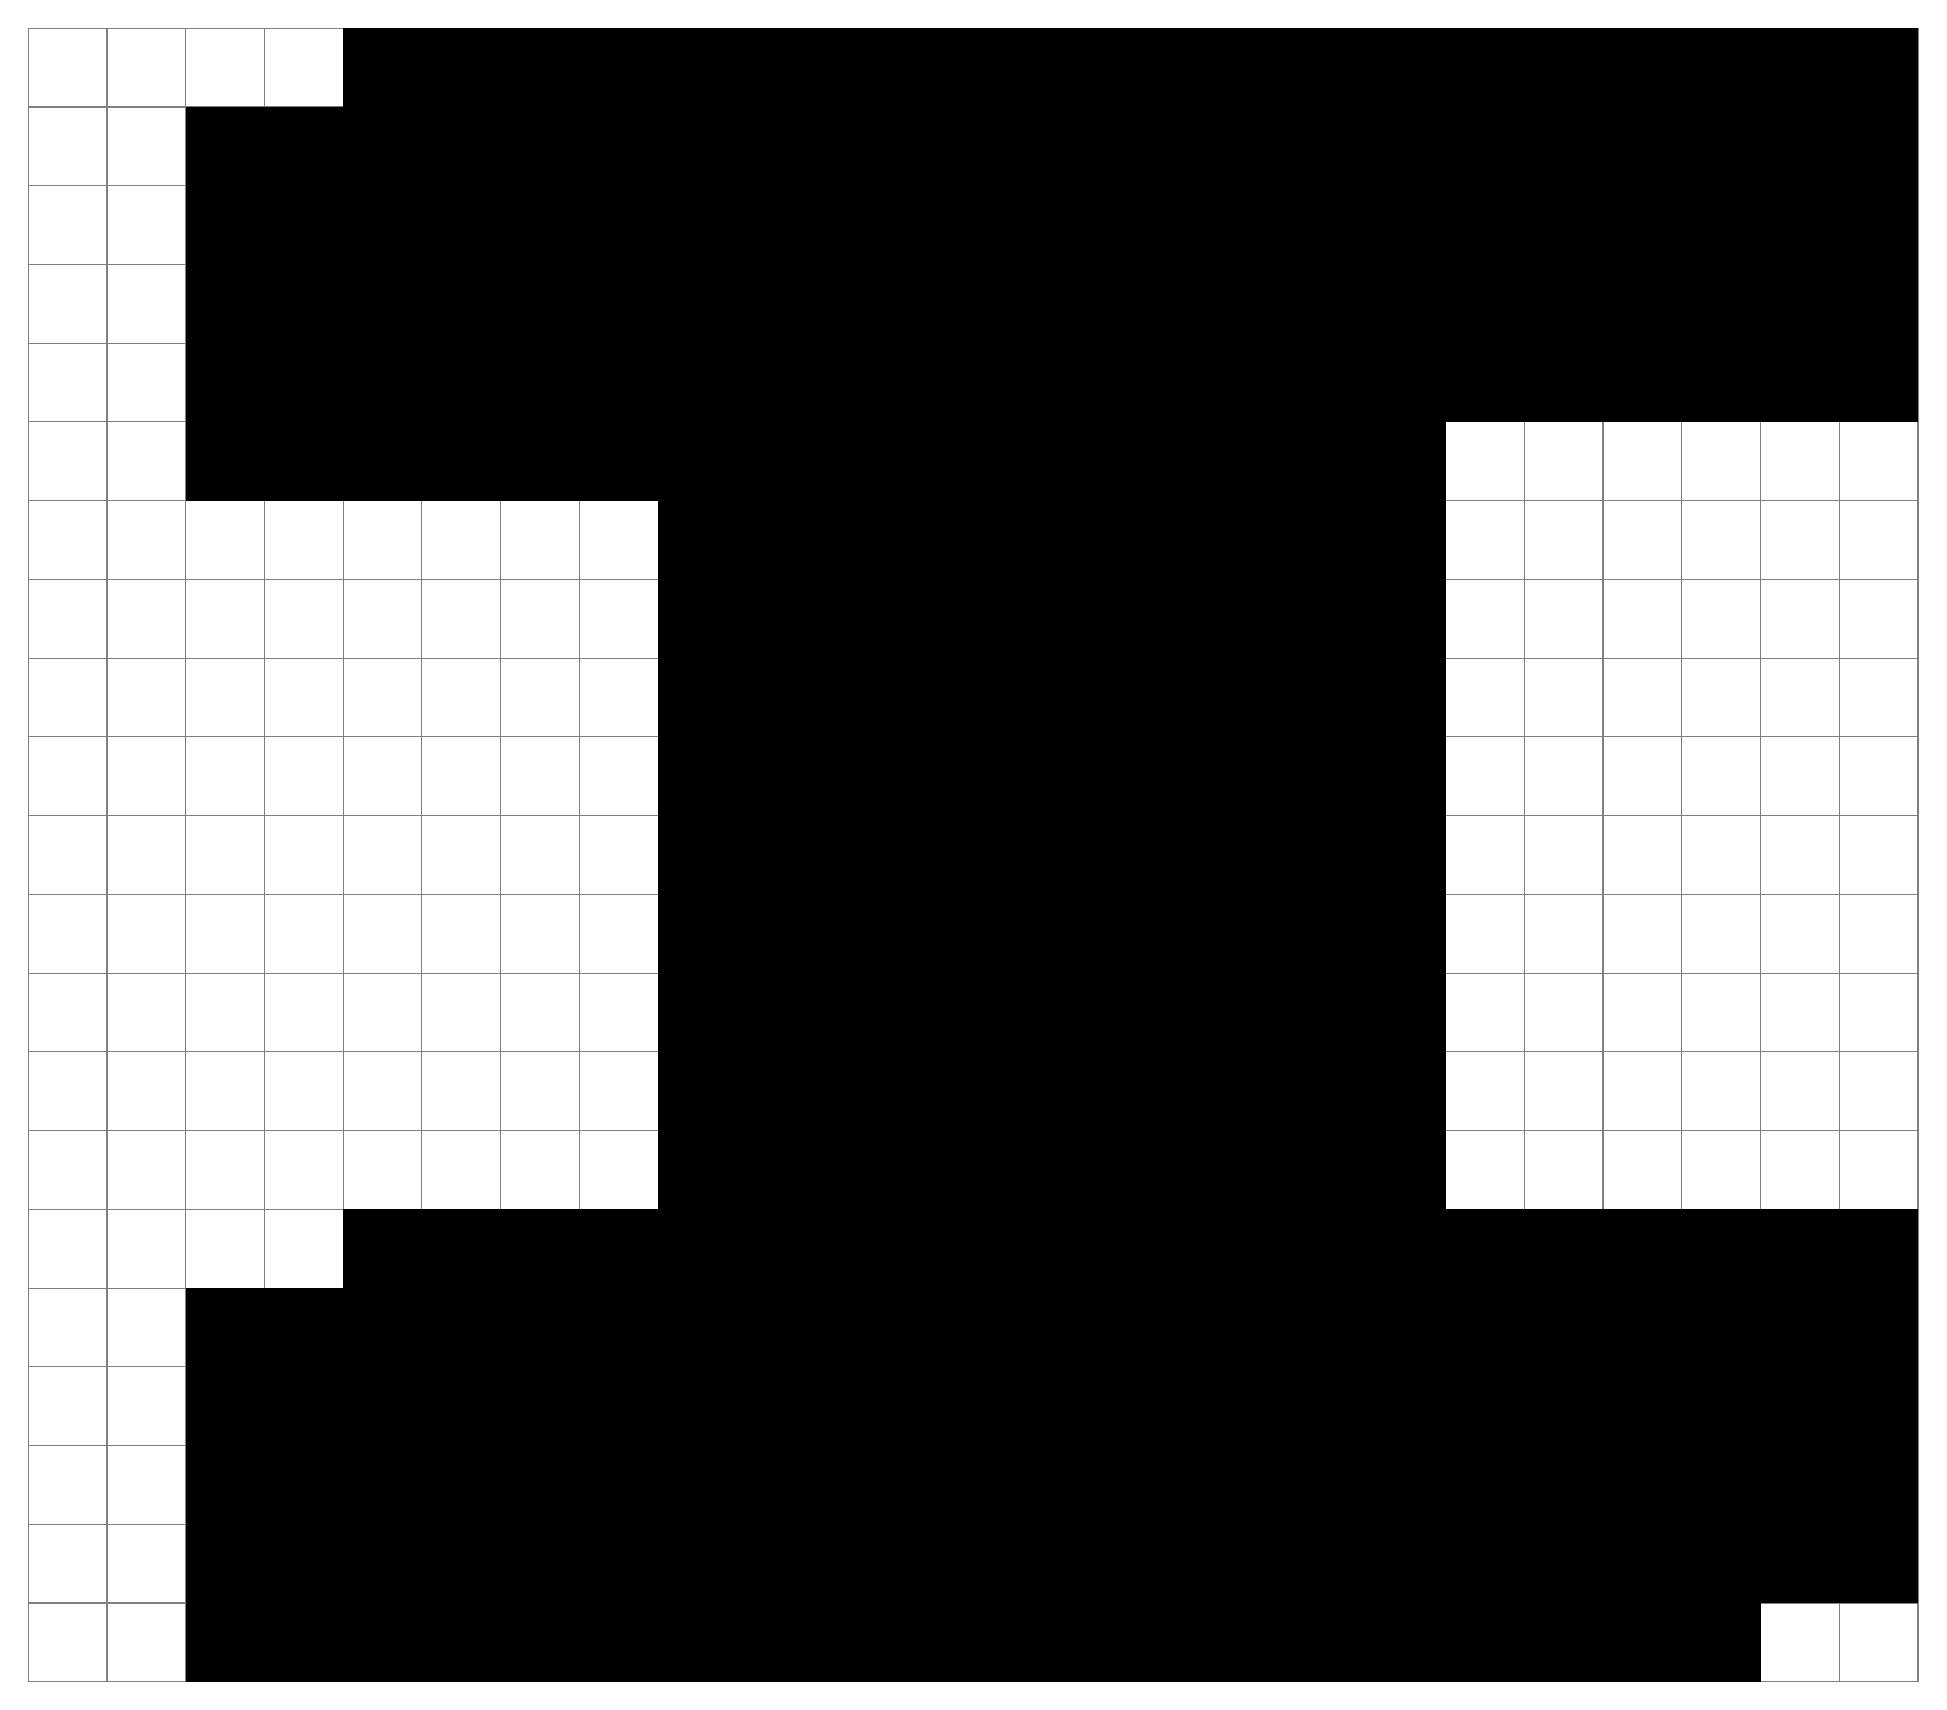
\begin{tikzpicture}

	\draw[step=1.0,gray,thin] (0,0) grid (24,21);
	\fill[\MULTICOLORTWO] (4,20) rectangle ++ (1,1);
	\fill[\MULTICOLORTWO] (5,20) rectangle ++ (1,1);
	\fill[\MULTICOLORTWO] (6,20) rectangle ++ (1,1);
	\fill[\MULTICOLORTWO] (7,20) rectangle ++ (1,1);
	\fill[\MULTICOLORTWO] (8,20) rectangle ++ (1,1);
	\fill[\MULTICOLORTWO] (9,20) rectangle ++ (1,1);
	\fill[\MULTICOLORTWO] (10,20) rectangle ++ (1,1);
	\fill[\MULTICOLORTWO] (11,20) rectangle ++ (1,1);
	\fill[\MULTICOLORTWO] (12,20) rectangle ++ (1,1);
	\fill[\MULTICOLORTWO] (13,20) rectangle ++ (1,1);
	\fill[\MULTICOLORTWO] (14,20) rectangle ++ (1,1);
	\fill[\MULTICOLORTWO] (15,20) rectangle ++ (1,1);
	\fill[\MULTICOLORTWO] (16,20) rectangle ++ (1,1);
	\fill[\MULTICOLORTWO] (17,20) rectangle ++ (1,1);
	\fill[\MULTICOLORTWO] (18,20) rectangle ++ (1,1);
	\fill[\MULTICOLORTWO] (19,20) rectangle ++ (1,1);
	\fill[\MULTICOLORTWO] (20,20) rectangle ++ (1,1);
	\fill[\MULTICOLORTWO] (21,20) rectangle ++ (1,1);
	\fill[\MULTICOLORTWO] (22,20) rectangle ++ (1,1);
	\fill[\MULTICOLORTWO] (23,20) rectangle ++ (1,1);
	\fill[\MULTICOLORONE] (2,19) rectangle ++ (1,1);
	\fill[\MULTICOLORONE] (3,19) rectangle ++ (1,1);
	\fill[\MULTICOLORTWO] (4,19) rectangle ++ (1,1);
	\fill[\MULTICOLORTWO] (5,19) rectangle ++ (1,1);
	\fill[\SPRITECOLOR] (6,19) rectangle ++ (1,1);
	\fill[\SPRITECOLOR] (7,19) rectangle ++ (1,1);
	\fill[\SPRITECOLOR] (8,19) rectangle ++ (1,1);
	\fill[\SPRITECOLOR] (9,19) rectangle ++ (1,1);
	\fill[\SPRITECOLOR] (10,19) rectangle ++ (1,1);
	\fill[\SPRITECOLOR] (11,19) rectangle ++ (1,1);
	\fill[\SPRITECOLOR] (12,19) rectangle ++ (1,1);
	\fill[\SPRITECOLOR] (13,19) rectangle ++ (1,1);
	\fill[\SPRITECOLOR] (14,19) rectangle ++ (1,1);
	\fill[\SPRITECOLOR] (15,19) rectangle ++ (1,1);
	\fill[\SPRITECOLOR] (16,19) rectangle ++ (1,1);
	\fill[\SPRITECOLOR] (17,19) rectangle ++ (1,1);
	\fill[\SPRITECOLOR] (18,19) rectangle ++ (1,1);
	\fill[\SPRITECOLOR] (19,19) rectangle ++ (1,1);
	\fill[\SPRITECOLOR] (20,19) rectangle ++ (1,1);
	\fill[\SPRITECOLOR] (21,19) rectangle ++ (1,1);
	\fill[\MULTICOLORTWO] (22,19) rectangle ++ (1,1);
	\fill[\MULTICOLORTWO] (23,19) rectangle ++ (1,1);
	\fill[\MULTICOLORONE] (2,18) rectangle ++ (1,1);
	\fill[\MULTICOLORONE] (3,18) rectangle ++ (1,1);
	\fill[\MULTICOLORTWO] (4,18) rectangle ++ (1,1);
	\fill[\MULTICOLORTWO] (5,18) rectangle ++ (1,1);
	\fill[\SPRITECOLOR] (6,18) rectangle ++ (1,1);
	\fill[\SPRITECOLOR] (7,18) rectangle ++ (1,1);
	\fill[\SPRITECOLOR] (8,18) rectangle ++ (1,1);
	\fill[\SPRITECOLOR] (9,18) rectangle ++ (1,1);
	\fill[\SPRITECOLOR] (10,18) rectangle ++ (1,1);
	\fill[\SPRITECOLOR] (11,18) rectangle ++ (1,1);
	\fill[\SPRITECOLOR] (12,18) rectangle ++ (1,1);
	\fill[\SPRITECOLOR] (13,18) rectangle ++ (1,1);
	\fill[\SPRITECOLOR] (14,18) rectangle ++ (1,1);
	\fill[\SPRITECOLOR] (15,18) rectangle ++ (1,1);
	\fill[\SPRITECOLOR] (16,18) rectangle ++ (1,1);
	\fill[\SPRITECOLOR] (17,18) rectangle ++ (1,1);
	\fill[\SPRITECOLOR] (18,18) rectangle ++ (1,1);
	\fill[\SPRITECOLOR] (19,18) rectangle ++ (1,1);
	\fill[\SPRITECOLOR] (20,18) rectangle ++ (1,1);
	\fill[\SPRITECOLOR] (21,18) rectangle ++ (1,1);
	\fill[\MULTICOLORTWO] (22,18) rectangle ++ (1,1);
	\fill[\MULTICOLORTWO] (23,18) rectangle ++ (1,1);
	\fill[\MULTICOLORONE] (2,17) rectangle ++ (1,1);
	\fill[\MULTICOLORONE] (3,17) rectangle ++ (1,1);
	\fill[\MULTICOLORTWO] (4,17) rectangle ++ (1,1);
	\fill[\MULTICOLORTWO] (5,17) rectangle ++ (1,1);
	\fill[\SPRITECOLOR] (6,17) rectangle ++ (1,1);
	\fill[\SPRITECOLOR] (7,17) rectangle ++ (1,1);
	\fill[\SPRITECOLOR] (8,17) rectangle ++ (1,1);
	\fill[\SPRITECOLOR] (9,17) rectangle ++ (1,1);
	\fill[\SPRITECOLOR] (10,17) rectangle ++ (1,1);
	\fill[\SPRITECOLOR] (11,17) rectangle ++ (1,1);
	\fill[\SPRITECOLOR] (12,17) rectangle ++ (1,1);
	\fill[\SPRITECOLOR] (13,17) rectangle ++ (1,1);
	\fill[\SPRITECOLOR] (14,17) rectangle ++ (1,1);
	\fill[\SPRITECOLOR] (15,17) rectangle ++ (1,1);
	\fill[\SPRITECOLOR] (16,17) rectangle ++ (1,1);
	\fill[\SPRITECOLOR] (17,17) rectangle ++ (1,1);
	\fill[\SPRITECOLOR] (18,17) rectangle ++ (1,1);
	\fill[\SPRITECOLOR] (19,17) rectangle ++ (1,1);
	\fill[\SPRITECOLOR] (20,17) rectangle ++ (1,1);
	\fill[\SPRITECOLOR] (21,17) rectangle ++ (1,1);
	\fill[\MULTICOLORTWO] (22,17) rectangle ++ (1,1);
	\fill[\MULTICOLORTWO] (23,17) rectangle ++ (1,1);
	\fill[\MULTICOLORONE] (2,16) rectangle ++ (1,1);
	\fill[\MULTICOLORONE] (3,16) rectangle ++ (1,1);
	\fill[\MULTICOLORTWO] (4,16) rectangle ++ (1,1);
	\fill[\MULTICOLORTWO] (5,16) rectangle ++ (1,1);
	\fill[\MULTICOLORTWO] (6,16) rectangle ++ (1,1);
	\fill[\MULTICOLORTWO] (7,16) rectangle ++ (1,1);
	\fill[\MULTICOLORTWO] (8,16) rectangle ++ (1,1);
	\fill[\MULTICOLORTWO] (9,16) rectangle ++ (1,1);
	\fill[\MULTICOLORTWO] (10,16) rectangle ++ (1,1);
	\fill[\MULTICOLORTWO] (11,16) rectangle ++ (1,1);
	\fill[\SPRITECOLOR] (12,16) rectangle ++ (1,1);
	\fill[\SPRITECOLOR] (13,16) rectangle ++ (1,1);
	\fill[\SPRITECOLOR] (14,16) rectangle ++ (1,1);
	\fill[\SPRITECOLOR] (15,16) rectangle ++ (1,1);
	\fill[\MULTICOLORTWO] (16,16) rectangle ++ (1,1);
	\fill[\MULTICOLORTWO] (17,16) rectangle ++ (1,1);
	\fill[\MULTICOLORTWO] (18,16) rectangle ++ (1,1);
	\fill[\MULTICOLORTWO] (19,16) rectangle ++ (1,1);
	\fill[\MULTICOLORTWO] (20,16) rectangle ++ (1,1);
	\fill[\MULTICOLORTWO] (21,16) rectangle ++ (1,1);
	\fill[\MULTICOLORTWO] (22,16) rectangle ++ (1,1);
	\fill[\MULTICOLORTWO] (23,16) rectangle ++ (1,1);
	\fill[\MULTICOLORONE] (2,15) rectangle ++ (1,1);
	\fill[\MULTICOLORONE] (3,15) rectangle ++ (1,1);
	\fill[\MULTICOLORONE] (4,15) rectangle ++ (1,1);
	\fill[\MULTICOLORONE] (5,15) rectangle ++ (1,1);
	\fill[\MULTICOLORONE] (6,15) rectangle ++ (1,1);
	\fill[\MULTICOLORONE] (7,15) rectangle ++ (1,1);
	\fill[\MULTICOLORONE] (8,15) rectangle ++ (1,1);
	\fill[\MULTICOLORONE] (9,15) rectangle ++ (1,1);
	\fill[\MULTICOLORTWO] (10,15) rectangle ++ (1,1);
	\fill[\MULTICOLORTWO] (11,15) rectangle ++ (1,1);
	\fill[\SPRITECOLOR] (12,15) rectangle ++ (1,1);
	\fill[\SPRITECOLOR] (13,15) rectangle ++ (1,1);
	\fill[\SPRITECOLOR] (14,15) rectangle ++ (1,1);
	\fill[\SPRITECOLOR] (15,15) rectangle ++ (1,1);
	\fill[\MULTICOLORTWO] (16,15) rectangle ++ (1,1);
	\fill[\MULTICOLORTWO] (17,15) rectangle ++ (1,1);
	\fill[\MULTICOLORONE] (8,14) rectangle ++ (1,1);
	\fill[\MULTICOLORONE] (9,14) rectangle ++ (1,1);
	\fill[\MULTICOLORTWO] (10,14) rectangle ++ (1,1);
	\fill[\MULTICOLORTWO] (11,14) rectangle ++ (1,1);
	\fill[\SPRITECOLOR] (12,14) rectangle ++ (1,1);
	\fill[\SPRITECOLOR] (13,14) rectangle ++ (1,1);
	\fill[\SPRITECOLOR] (14,14) rectangle ++ (1,1);
	\fill[\SPRITECOLOR] (15,14) rectangle ++ (1,1);
	\fill[\MULTICOLORTWO] (16,14) rectangle ++ (1,1);
	\fill[\MULTICOLORTWO] (17,14) rectangle ++ (1,1);
	\fill[\MULTICOLORONE] (8,13) rectangle ++ (1,1);
	\fill[\MULTICOLORONE] (9,13) rectangle ++ (1,1);
	\fill[\MULTICOLORTWO] (10,13) rectangle ++ (1,1);
	\fill[\MULTICOLORTWO] (11,13) rectangle ++ (1,1);
	\fill[\SPRITECOLOR] (12,13) rectangle ++ (1,1);
	\fill[\SPRITECOLOR] (13,13) rectangle ++ (1,1);
	\fill[\SPRITECOLOR] (14,13) rectangle ++ (1,1);
	\fill[\SPRITECOLOR] (15,13) rectangle ++ (1,1);
	\fill[\MULTICOLORTWO] (16,13) rectangle ++ (1,1);
	\fill[\MULTICOLORTWO] (17,13) rectangle ++ (1,1);
	\fill[\MULTICOLORONE] (8,12) rectangle ++ (1,1);
	\fill[\MULTICOLORONE] (9,12) rectangle ++ (1,1);
	\fill[\MULTICOLORTWO] (10,12) rectangle ++ (1,1);
	\fill[\MULTICOLORTWO] (11,12) rectangle ++ (1,1);
	\fill[\SPRITECOLOR] (12,12) rectangle ++ (1,1);
	\fill[\SPRITECOLOR] (13,12) rectangle ++ (1,1);
	\fill[\SPRITECOLOR] (14,12) rectangle ++ (1,1);
	\fill[\SPRITECOLOR] (15,12) rectangle ++ (1,1);
	\fill[\MULTICOLORTWO] (16,12) rectangle ++ (1,1);
	\fill[\MULTICOLORTWO] (17,12) rectangle ++ (1,1);
	\fill[\MULTICOLORONE] (8,11) rectangle ++ (1,1);
	\fill[\MULTICOLORONE] (9,11) rectangle ++ (1,1);
	\fill[\MULTICOLORTWO] (10,11) rectangle ++ (1,1);
	\fill[\MULTICOLORTWO] (11,11) rectangle ++ (1,1);
	\fill[\SPRITECOLOR] (12,11) rectangle ++ (1,1);
	\fill[\SPRITECOLOR] (13,11) rectangle ++ (1,1);
	\fill[\SPRITECOLOR] (14,11) rectangle ++ (1,1);
	\fill[\SPRITECOLOR] (15,11) rectangle ++ (1,1);
	\fill[\MULTICOLORTWO] (16,11) rectangle ++ (1,1);
	\fill[\MULTICOLORTWO] (17,11) rectangle ++ (1,1);
	\fill[\MULTICOLORONE] (8,10) rectangle ++ (1,1);
	\fill[\MULTICOLORONE] (9,10) rectangle ++ (1,1);
	\fill[\MULTICOLORTWO] (10,10) rectangle ++ (1,1);
	\fill[\MULTICOLORTWO] (11,10) rectangle ++ (1,1);
	\fill[\SPRITECOLOR] (12,10) rectangle ++ (1,1);
	\fill[\SPRITECOLOR] (13,10) rectangle ++ (1,1);
	\fill[\SPRITECOLOR] (14,10) rectangle ++ (1,1);
	\fill[\SPRITECOLOR] (15,10) rectangle ++ (1,1);
	\fill[\MULTICOLORTWO] (16,10) rectangle ++ (1,1);
	\fill[\MULTICOLORTWO] (17,10) rectangle ++ (1,1);
	\fill[\MULTICOLORONE] (8,9) rectangle ++ (1,1);
	\fill[\MULTICOLORONE] (9,9) rectangle ++ (1,1);
	\fill[\MULTICOLORTWO] (10,9) rectangle ++ (1,1);
	\fill[\MULTICOLORTWO] (11,9) rectangle ++ (1,1);
	\fill[\SPRITECOLOR] (12,9) rectangle ++ (1,1);
	\fill[\SPRITECOLOR] (13,9) rectangle ++ (1,1);
	\fill[\SPRITECOLOR] (14,9) rectangle ++ (1,1);
	\fill[\SPRITECOLOR] (15,9) rectangle ++ (1,1);
	\fill[\MULTICOLORTWO] (16,9) rectangle ++ (1,1);
	\fill[\MULTICOLORTWO] (17,9) rectangle ++ (1,1);
	\fill[\MULTICOLORONE] (8,8) rectangle ++ (1,1);
	\fill[\MULTICOLORONE] (9,8) rectangle ++ (1,1);
	\fill[\MULTICOLORTWO] (10,8) rectangle ++ (1,1);
	\fill[\MULTICOLORTWO] (11,8) rectangle ++ (1,1);
	\fill[\SPRITECOLOR] (12,8) rectangle ++ (1,1);
	\fill[\SPRITECOLOR] (13,8) rectangle ++ (1,1);
	\fill[\SPRITECOLOR] (14,8) rectangle ++ (1,1);
	\fill[\SPRITECOLOR] (15,8) rectangle ++ (1,1);
	\fill[\MULTICOLORTWO] (16,8) rectangle ++ (1,1);
	\fill[\MULTICOLORTWO] (17,8) rectangle ++ (1,1);
	\fill[\MULTICOLORONE] (8,7) rectangle ++ (1,1);
	\fill[\MULTICOLORONE] (9,7) rectangle ++ (1,1);
	\fill[\MULTICOLORTWO] (10,7) rectangle ++ (1,1);
	\fill[\MULTICOLORTWO] (11,7) rectangle ++ (1,1);
	\fill[\SPRITECOLOR] (12,7) rectangle ++ (1,1);
	\fill[\SPRITECOLOR] (13,7) rectangle ++ (1,1);
	\fill[\SPRITECOLOR] (14,7) rectangle ++ (1,1);
	\fill[\SPRITECOLOR] (15,7) rectangle ++ (1,1);
	\fill[\MULTICOLORTWO] (16,7) rectangle ++ (1,1);
	\fill[\MULTICOLORTWO] (17,7) rectangle ++ (1,1);
	\fill[\MULTICOLORONE] (8,6) rectangle ++ (1,1);
	\fill[\MULTICOLORONE] (9,6) rectangle ++ (1,1);
	\fill[\MULTICOLORTWO] (10,6) rectangle ++ (1,1);
	\fill[\MULTICOLORTWO] (11,6) rectangle ++ (1,1);
	\fill[\SPRITECOLOR] (12,6) rectangle ++ (1,1);
	\fill[\SPRITECOLOR] (13,6) rectangle ++ (1,1);
	\fill[\SPRITECOLOR] (14,6) rectangle ++ (1,1);
	\fill[\SPRITECOLOR] (15,6) rectangle ++ (1,1);
	\fill[\MULTICOLORTWO] (16,6) rectangle ++ (1,1);
	\fill[\MULTICOLORTWO] (17,6) rectangle ++ (1,1);
	\fill[\MULTICOLORTWO] (4,5) rectangle ++ (1,1);
	\fill[\MULTICOLORTWO] (5,5) rectangle ++ (1,1);
	\fill[\MULTICOLORTWO] (6,5) rectangle ++ (1,1);
	\fill[\MULTICOLORTWO] (7,5) rectangle ++ (1,1);
	\fill[\MULTICOLORTWO] (8,5) rectangle ++ (1,1);
	\fill[\MULTICOLORTWO] (9,5) rectangle ++ (1,1);
	\fill[\MULTICOLORTWO] (10,5) rectangle ++ (1,1);
	\fill[\MULTICOLORTWO] (11,5) rectangle ++ (1,1);
	\fill[\SPRITECOLOR] (12,5) rectangle ++ (1,1);
	\fill[\SPRITECOLOR] (13,5) rectangle ++ (1,1);
	\fill[\SPRITECOLOR] (14,5) rectangle ++ (1,1);
	\fill[\SPRITECOLOR] (15,5) rectangle ++ (1,1);
	\fill[\MULTICOLORTWO] (16,5) rectangle ++ (1,1);
	\fill[\MULTICOLORTWO] (17,5) rectangle ++ (1,1);
	\fill[\MULTICOLORTWO] (18,5) rectangle ++ (1,1);
	\fill[\MULTICOLORTWO] (19,5) rectangle ++ (1,1);
	\fill[\MULTICOLORTWO] (20,5) rectangle ++ (1,1);
	\fill[\MULTICOLORTWO] (21,5) rectangle ++ (1,1);
	\fill[\MULTICOLORTWO] (22,5) rectangle ++ (1,1);
	\fill[\MULTICOLORTWO] (23,5) rectangle ++ (1,1);
	\fill[\MULTICOLORONE] (2,4) rectangle ++ (1,1);
	\fill[\MULTICOLORONE] (3,4) rectangle ++ (1,1);
	\fill[\MULTICOLORTWO] (4,4) rectangle ++ (1,1);
	\fill[\MULTICOLORTWO] (5,4) rectangle ++ (1,1);
	\fill[\SPRITECOLOR] (6,4) rectangle ++ (1,1);
	\fill[\SPRITECOLOR] (7,4) rectangle ++ (1,1);
	\fill[\SPRITECOLOR] (8,4) rectangle ++ (1,1);
	\fill[\SPRITECOLOR] (9,4) rectangle ++ (1,1);
	\fill[\SPRITECOLOR] (10,4) rectangle ++ (1,1);
	\fill[\SPRITECOLOR] (11,4) rectangle ++ (1,1);
	\fill[\SPRITECOLOR] (12,4) rectangle ++ (1,1);
	\fill[\SPRITECOLOR] (13,4) rectangle ++ (1,1);
	\fill[\SPRITECOLOR] (14,4) rectangle ++ (1,1);
	\fill[\SPRITECOLOR] (15,4) rectangle ++ (1,1);
	\fill[\SPRITECOLOR] (16,4) rectangle ++ (1,1);
	\fill[\SPRITECOLOR] (17,4) rectangle ++ (1,1);
	\fill[\SPRITECOLOR] (18,4) rectangle ++ (1,1);
	\fill[\SPRITECOLOR] (19,4) rectangle ++ (1,1);
	\fill[\SPRITECOLOR] (20,4) rectangle ++ (1,1);
	\fill[\SPRITECOLOR] (21,4) rectangle ++ (1,1);
	\fill[\MULTICOLORTWO] (22,4) rectangle ++ (1,1);
	\fill[\MULTICOLORTWO] (23,4) rectangle ++ (1,1);
	\fill[\MULTICOLORONE] (2,3) rectangle ++ (1,1);
	\fill[\MULTICOLORONE] (3,3) rectangle ++ (1,1);
	\fill[\MULTICOLORTWO] (4,3) rectangle ++ (1,1);
	\fill[\MULTICOLORTWO] (5,3) rectangle ++ (1,1);
	\fill[\SPRITECOLOR] (6,3) rectangle ++ (1,1);
	\fill[\SPRITECOLOR] (7,3) rectangle ++ (1,1);
	\fill[\SPRITECOLOR] (8,3) rectangle ++ (1,1);
	\fill[\SPRITECOLOR] (9,3) rectangle ++ (1,1);
	\fill[\SPRITECOLOR] (10,3) rectangle ++ (1,1);
	\fill[\SPRITECOLOR] (11,3) rectangle ++ (1,1);
	\fill[\SPRITECOLOR] (12,3) rectangle ++ (1,1);
	\fill[\SPRITECOLOR] (13,3) rectangle ++ (1,1);
	\fill[\SPRITECOLOR] (14,3) rectangle ++ (1,1);
	\fill[\SPRITECOLOR] (15,3) rectangle ++ (1,1);
	\fill[\SPRITECOLOR] (16,3) rectangle ++ (1,1);
	\fill[\SPRITECOLOR] (17,3) rectangle ++ (1,1);
	\fill[\SPRITECOLOR] (18,3) rectangle ++ (1,1);
	\fill[\SPRITECOLOR] (19,3) rectangle ++ (1,1);
	\fill[\SPRITECOLOR] (20,3) rectangle ++ (1,1);
	\fill[\SPRITECOLOR] (21,3) rectangle ++ (1,1);
	\fill[\MULTICOLORTWO] (22,3) rectangle ++ (1,1);
	\fill[\MULTICOLORTWO] (23,3) rectangle ++ (1,1);
	\fill[\MULTICOLORONE] (2,2) rectangle ++ (1,1);
	\fill[\MULTICOLORONE] (3,2) rectangle ++ (1,1);
	\fill[\MULTICOLORTWO] (4,2) rectangle ++ (1,1);
	\fill[\MULTICOLORTWO] (5,2) rectangle ++ (1,1);
	\fill[\SPRITECOLOR] (6,2) rectangle ++ (1,1);
	\fill[\SPRITECOLOR] (7,2) rectangle ++ (1,1);
	\fill[\SPRITECOLOR] (8,2) rectangle ++ (1,1);
	\fill[\SPRITECOLOR] (9,2) rectangle ++ (1,1);
	\fill[\SPRITECOLOR] (10,2) rectangle ++ (1,1);
	\fill[\SPRITECOLOR] (11,2) rectangle ++ (1,1);
	\fill[\SPRITECOLOR] (12,2) rectangle ++ (1,1);
	\fill[\SPRITECOLOR] (13,2) rectangle ++ (1,1);
	\fill[\SPRITECOLOR] (14,2) rectangle ++ (1,1);
	\fill[\SPRITECOLOR] (15,2) rectangle ++ (1,1);
	\fill[\SPRITECOLOR] (16,2) rectangle ++ (1,1);
	\fill[\SPRITECOLOR] (17,2) rectangle ++ (1,1);
	\fill[\SPRITECOLOR] (18,2) rectangle ++ (1,1);
	\fill[\SPRITECOLOR] (19,2) rectangle ++ (1,1);
	\fill[\SPRITECOLOR] (20,2) rectangle ++ (1,1);
	\fill[\SPRITECOLOR] (21,2) rectangle ++ (1,1);
	\fill[\MULTICOLORTWO] (22,2) rectangle ++ (1,1);
	\fill[\MULTICOLORTWO] (23,2) rectangle ++ (1,1);
	\fill[\MULTICOLORONE] (2,1) rectangle ++ (1,1);
	\fill[\MULTICOLORONE] (3,1) rectangle ++ (1,1);
	\fill[\MULTICOLORTWO] (4,1) rectangle ++ (1,1);
	\fill[\MULTICOLORTWO] (5,1) rectangle ++ (1,1);
	\fill[\MULTICOLORTWO] (6,1) rectangle ++ (1,1);
	\fill[\MULTICOLORTWO] (7,1) rectangle ++ (1,1);
	\fill[\MULTICOLORTWO] (8,1) rectangle ++ (1,1);
	\fill[\MULTICOLORTWO] (9,1) rectangle ++ (1,1);
	\fill[\MULTICOLORTWO] (10,1) rectangle ++ (1,1);
	\fill[\MULTICOLORTWO] (11,1) rectangle ++ (1,1);
	\fill[\MULTICOLORTWO] (12,1) rectangle ++ (1,1);
	\fill[\MULTICOLORTWO] (13,1) rectangle ++ (1,1);
	\fill[\MULTICOLORTWO] (14,1) rectangle ++ (1,1);
	\fill[\MULTICOLORTWO] (15,1) rectangle ++ (1,1);
	\fill[\MULTICOLORTWO] (16,1) rectangle ++ (1,1);
	\fill[\MULTICOLORTWO] (17,1) rectangle ++ (1,1);
	\fill[\MULTICOLORTWO] (18,1) rectangle ++ (1,1);
	\fill[\MULTICOLORTWO] (19,1) rectangle ++ (1,1);
	\fill[\MULTICOLORTWO] (20,1) rectangle ++ (1,1);
	\fill[\MULTICOLORTWO] (21,1) rectangle ++ (1,1);
	\fill[\MULTICOLORTWO] (22,1) rectangle ++ (1,1);
	\fill[\MULTICOLORTWO] (23,1) rectangle ++ (1,1);
	\fill[\MULTICOLORONE] (2,0) rectangle ++ (1,1);
	\fill[\MULTICOLORONE] (3,0) rectangle ++ (1,1);
	\fill[\MULTICOLORONE] (4,0) rectangle ++ (1,1);
	\fill[\MULTICOLORONE] (5,0) rectangle ++ (1,1);
	\fill[\MULTICOLORONE] (6,0) rectangle ++ (1,1);
	\fill[\MULTICOLORONE] (7,0) rectangle ++ (1,1);
	\fill[\MULTICOLORONE] (8,0) rectangle ++ (1,1);
	\fill[\MULTICOLORONE] (9,0) rectangle ++ (1,1);
	\fill[\MULTICOLORONE] (10,0) rectangle ++ (1,1);
	\fill[\MULTICOLORONE] (11,0) rectangle ++ (1,1);
	\fill[\MULTICOLORONE] (12,0) rectangle ++ (1,1);
	\fill[\MULTICOLORONE] (13,0) rectangle ++ (1,1);
	\fill[\MULTICOLORONE] (14,0) rectangle ++ (1,1);
	\fill[\MULTICOLORONE] (15,0) rectangle ++ (1,1);
	\fill[\MULTICOLORONE] (16,0) rectangle ++ (1,1);
	\fill[\MULTICOLORONE] (17,0) rectangle ++ (1,1);
	\fill[\MULTICOLORONE] (18,0) rectangle ++ (1,1);
	\fill[\MULTICOLORONE] (19,0) rectangle ++ (1,1);
	\fill[\MULTICOLORONE] (20,0) rectangle ++ (1,1);
	\fill[\MULTICOLORONE] (21,0) rectangle ++ (1,1);

      \end{tikzpicture}
    \end{adjustbox}
  }\caption{BIG\_I}
\end{figure}

	\end{subfigure}
} &
\makecell[l]{
	\begin{subfigure}{0.3\textwidth}
    \def\MULTICOLORONE{gray}
    \def\MULTICOLORTWO{black}
    \def\SPRITECOLOR{green}
		
\begin{figure}[H]
  {
    \setlength{\tabcolsep}{3.0pt}
    \setlength\cmidrulewidth{\heavyrulewidth} % Make cmidrule = 
    \begin{adjustbox}{width=3cm,center}
      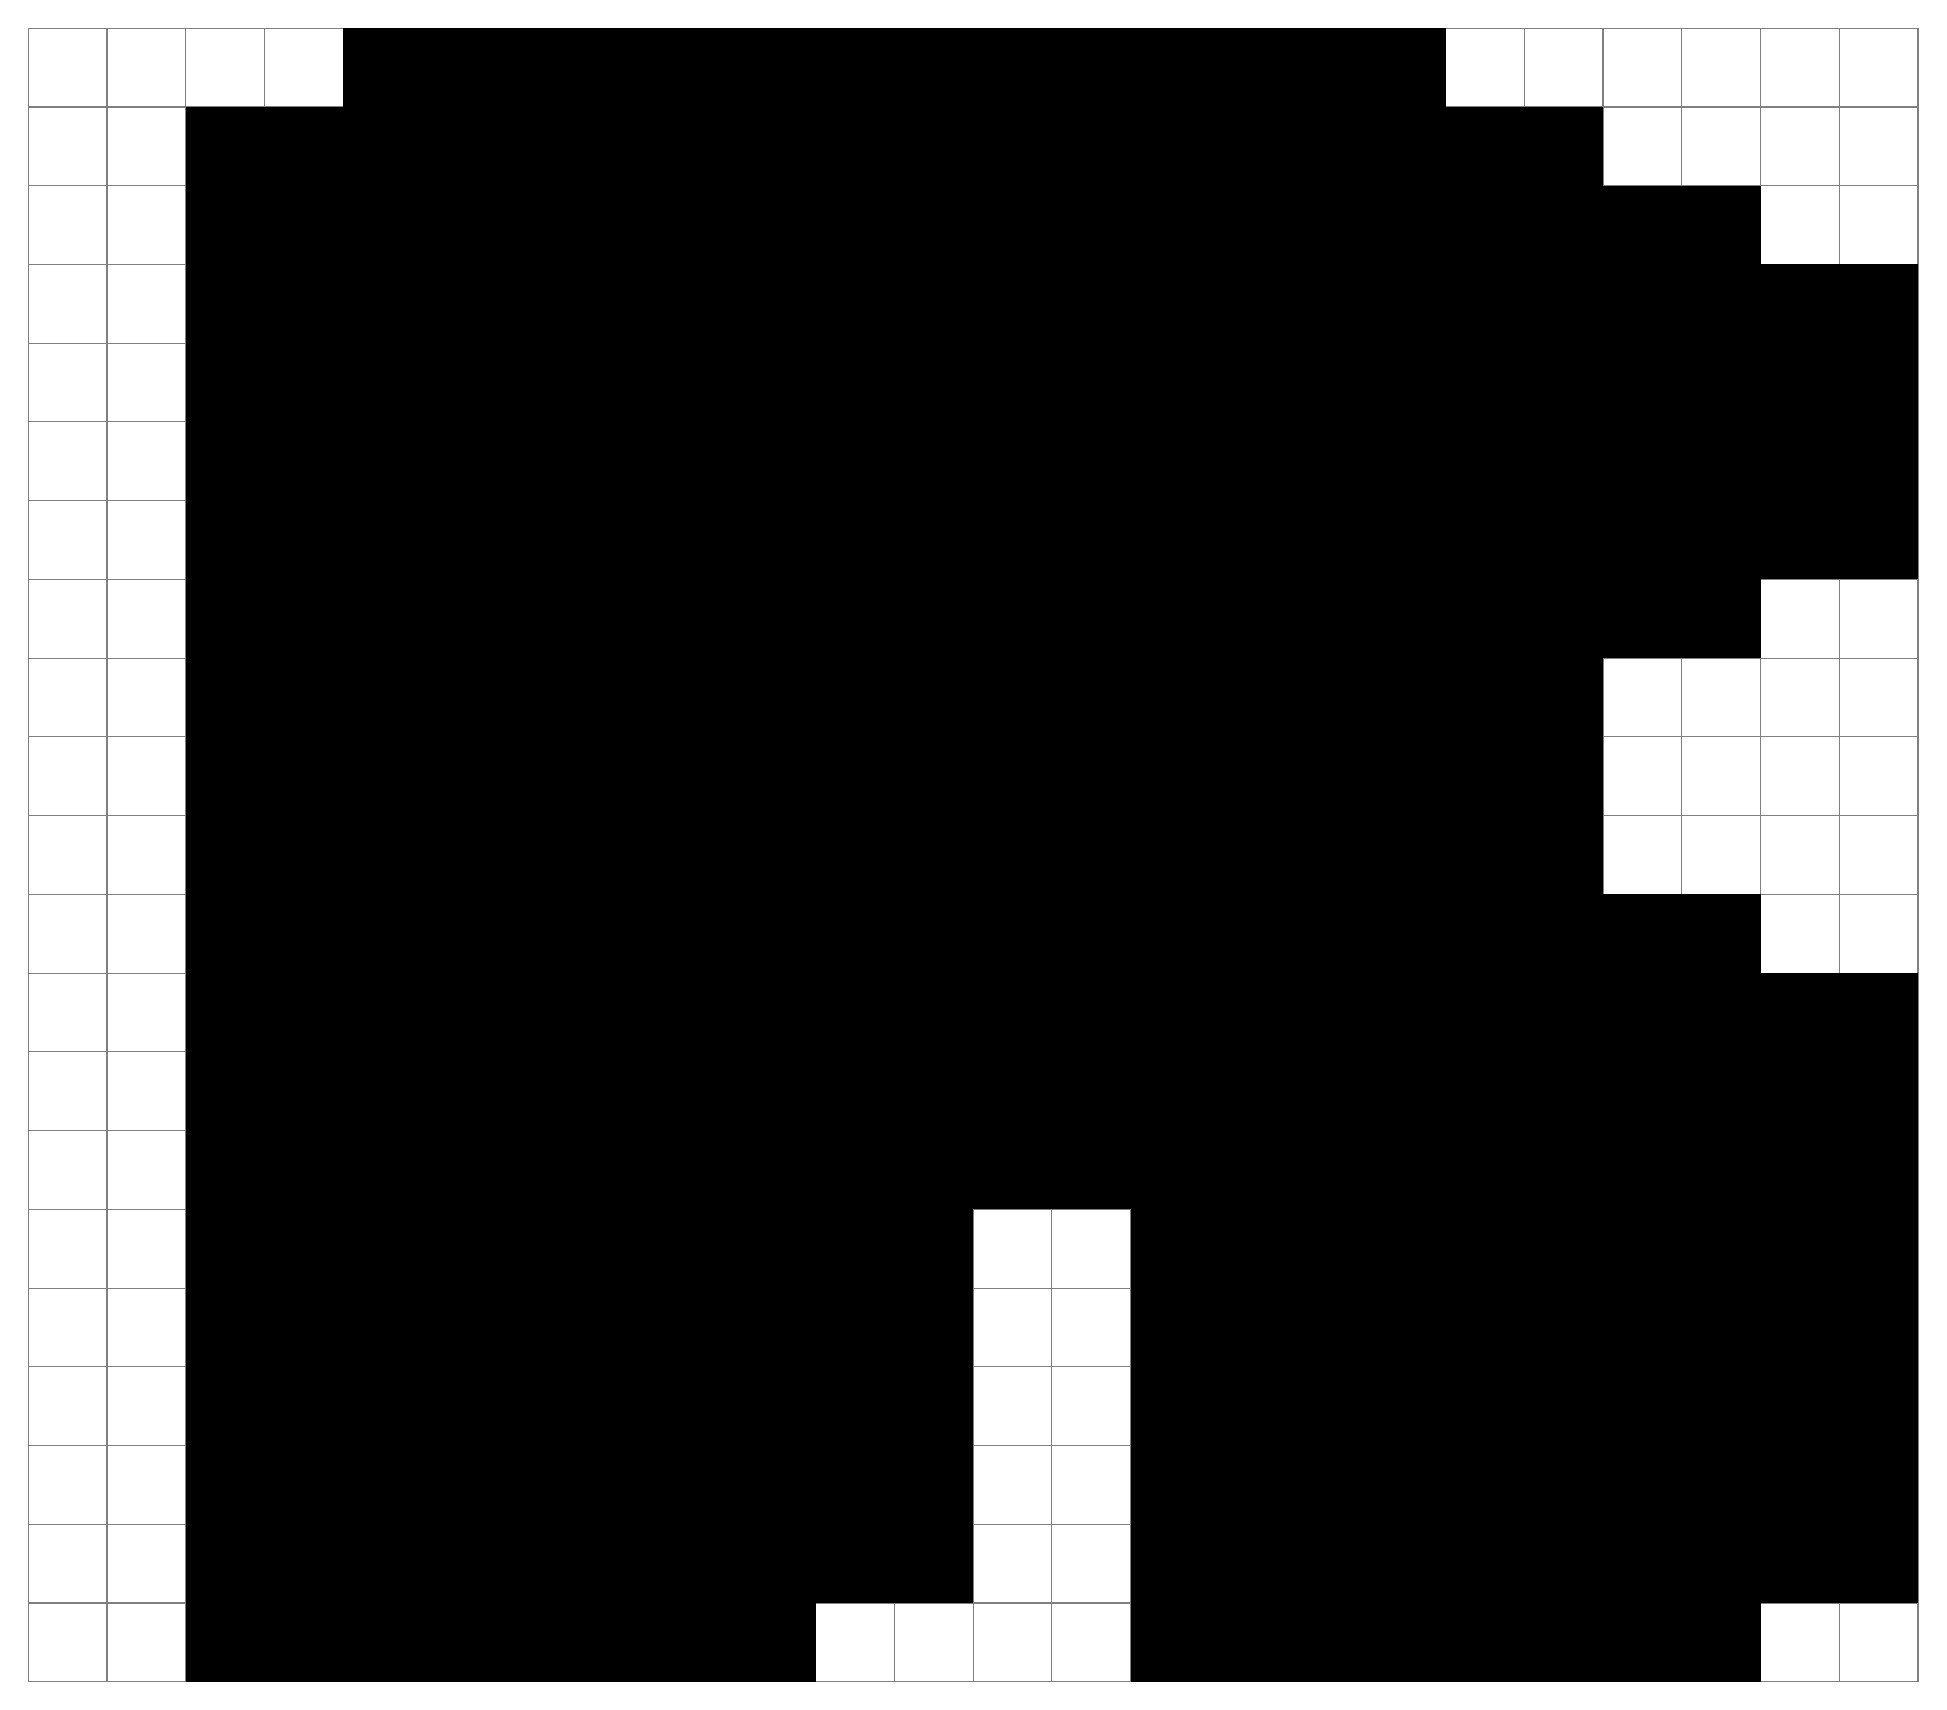
\begin{tikzpicture}

	\draw[step=1.0,gray,thin] (0,0) grid (24,21);
	\fill[\MULTICOLORTWO] (4,20) rectangle ++ (1,1);
	\fill[\MULTICOLORTWO] (5,20) rectangle ++ (1,1);
	\fill[\MULTICOLORTWO] (6,20) rectangle ++ (1,1);
	\fill[\MULTICOLORTWO] (7,20) rectangle ++ (1,1);
	\fill[\MULTICOLORTWO] (8,20) rectangle ++ (1,1);
	\fill[\MULTICOLORTWO] (9,20) rectangle ++ (1,1);
	\fill[\MULTICOLORTWO] (10,20) rectangle ++ (1,1);
	\fill[\MULTICOLORTWO] (11,20) rectangle ++ (1,1);
	\fill[\MULTICOLORTWO] (12,20) rectangle ++ (1,1);
	\fill[\MULTICOLORTWO] (13,20) rectangle ++ (1,1);
	\fill[\MULTICOLORTWO] (14,20) rectangle ++ (1,1);
	\fill[\MULTICOLORTWO] (15,20) rectangle ++ (1,1);
	\fill[\MULTICOLORTWO] (16,20) rectangle ++ (1,1);
	\fill[\MULTICOLORTWO] (17,20) rectangle ++ (1,1);
	\fill[\MULTICOLORONE] (2,19) rectangle ++ (1,1);
	\fill[\MULTICOLORONE] (3,19) rectangle ++ (1,1);
	\fill[\MULTICOLORTWO] (4,19) rectangle ++ (1,1);
	\fill[\MULTICOLORTWO] (5,19) rectangle ++ (1,1);
	\fill[\SPRITECOLOR] (6,19) rectangle ++ (1,1);
	\fill[\SPRITECOLOR] (7,19) rectangle ++ (1,1);
	\fill[\SPRITECOLOR] (8,19) rectangle ++ (1,1);
	\fill[\SPRITECOLOR] (9,19) rectangle ++ (1,1);
	\fill[\SPRITECOLOR] (10,19) rectangle ++ (1,1);
	\fill[\SPRITECOLOR] (11,19) rectangle ++ (1,1);
	\fill[\SPRITECOLOR] (12,19) rectangle ++ (1,1);
	\fill[\SPRITECOLOR] (13,19) rectangle ++ (1,1);
	\fill[\SPRITECOLOR] (14,19) rectangle ++ (1,1);
	\fill[\SPRITECOLOR] (15,19) rectangle ++ (1,1);
	\fill[\SPRITECOLOR] (16,19) rectangle ++ (1,1);
	\fill[\SPRITECOLOR] (17,19) rectangle ++ (1,1);
	\fill[\MULTICOLORTWO] (18,19) rectangle ++ (1,1);
	\fill[\MULTICOLORTWO] (19,19) rectangle ++ (1,1);
	\fill[\MULTICOLORONE] (2,18) rectangle ++ (1,1);
	\fill[\MULTICOLORONE] (3,18) rectangle ++ (1,1);
	\fill[\MULTICOLORTWO] (4,18) rectangle ++ (1,1);
	\fill[\MULTICOLORTWO] (5,18) rectangle ++ (1,1);
	\fill[\SPRITECOLOR] (6,18) rectangle ++ (1,1);
	\fill[\SPRITECOLOR] (7,18) rectangle ++ (1,1);
	\fill[\SPRITECOLOR] (8,18) rectangle ++ (1,1);
	\fill[\SPRITECOLOR] (9,18) rectangle ++ (1,1);
	\fill[\SPRITECOLOR] (10,18) rectangle ++ (1,1);
	\fill[\SPRITECOLOR] (11,18) rectangle ++ (1,1);
	\fill[\SPRITECOLOR] (12,18) rectangle ++ (1,1);
	\fill[\SPRITECOLOR] (13,18) rectangle ++ (1,1);
	\fill[\SPRITECOLOR] (14,18) rectangle ++ (1,1);
	\fill[\SPRITECOLOR] (15,18) rectangle ++ (1,1);
	\fill[\SPRITECOLOR] (16,18) rectangle ++ (1,1);
	\fill[\SPRITECOLOR] (17,18) rectangle ++ (1,1);
	\fill[\SPRITECOLOR] (18,18) rectangle ++ (1,1);
	\fill[\SPRITECOLOR] (19,18) rectangle ++ (1,1);
	\fill[\MULTICOLORTWO] (20,18) rectangle ++ (1,1);
	\fill[\MULTICOLORTWO] (21,18) rectangle ++ (1,1);
	\fill[\MULTICOLORONE] (2,17) rectangle ++ (1,1);
	\fill[\MULTICOLORONE] (3,17) rectangle ++ (1,1);
	\fill[\MULTICOLORTWO] (4,17) rectangle ++ (1,1);
	\fill[\MULTICOLORTWO] (5,17) rectangle ++ (1,1);
	\fill[\SPRITECOLOR] (6,17) rectangle ++ (1,1);
	\fill[\SPRITECOLOR] (7,17) rectangle ++ (1,1);
	\fill[\SPRITECOLOR] (8,17) rectangle ++ (1,1);
	\fill[\SPRITECOLOR] (9,17) rectangle ++ (1,1);
	\fill[\SPRITECOLOR] (10,17) rectangle ++ (1,1);
	\fill[\SPRITECOLOR] (11,17) rectangle ++ (1,1);
	\fill[\SPRITECOLOR] (12,17) rectangle ++ (1,1);
	\fill[\SPRITECOLOR] (13,17) rectangle ++ (1,1);
	\fill[\SPRITECOLOR] (14,17) rectangle ++ (1,1);
	\fill[\SPRITECOLOR] (15,17) rectangle ++ (1,1);
	\fill[\SPRITECOLOR] (16,17) rectangle ++ (1,1);
	\fill[\SPRITECOLOR] (17,17) rectangle ++ (1,1);
	\fill[\SPRITECOLOR] (18,17) rectangle ++ (1,1);
	\fill[\SPRITECOLOR] (19,17) rectangle ++ (1,1);
	\fill[\SPRITECOLOR] (20,17) rectangle ++ (1,1);
	\fill[\SPRITECOLOR] (21,17) rectangle ++ (1,1);
	\fill[\MULTICOLORTWO] (22,17) rectangle ++ (1,1);
	\fill[\MULTICOLORTWO] (23,17) rectangle ++ (1,1);
	\fill[\MULTICOLORONE] (2,16) rectangle ++ (1,1);
	\fill[\MULTICOLORONE] (3,16) rectangle ++ (1,1);
	\fill[\MULTICOLORTWO] (4,16) rectangle ++ (1,1);
	\fill[\MULTICOLORTWO] (5,16) rectangle ++ (1,1);
	\fill[\SPRITECOLOR] (6,16) rectangle ++ (1,1);
	\fill[\SPRITECOLOR] (7,16) rectangle ++ (1,1);
	\fill[\SPRITECOLOR] (8,16) rectangle ++ (1,1);
	\fill[\SPRITECOLOR] (9,16) rectangle ++ (1,1);
	\fill[\MULTICOLORTWO] (10,16) rectangle ++ (1,1);
	\fill[\MULTICOLORTWO] (11,16) rectangle ++ (1,1);
	\fill[\MULTICOLORTWO] (12,16) rectangle ++ (1,1);
	\fill[\MULTICOLORTWO] (13,16) rectangle ++ (1,1);
	\fill[\SPRITECOLOR] (14,16) rectangle ++ (1,1);
	\fill[\SPRITECOLOR] (15,16) rectangle ++ (1,1);
	\fill[\SPRITECOLOR] (16,16) rectangle ++ (1,1);
	\fill[\SPRITECOLOR] (17,16) rectangle ++ (1,1);
	\fill[\SPRITECOLOR] (18,16) rectangle ++ (1,1);
	\fill[\SPRITECOLOR] (19,16) rectangle ++ (1,1);
	\fill[\SPRITECOLOR] (20,16) rectangle ++ (1,1);
	\fill[\SPRITECOLOR] (21,16) rectangle ++ (1,1);
	\fill[\MULTICOLORTWO] (22,16) rectangle ++ (1,1);
	\fill[\MULTICOLORTWO] (23,16) rectangle ++ (1,1);
	\fill[\MULTICOLORONE] (2,15) rectangle ++ (1,1);
	\fill[\MULTICOLORONE] (3,15) rectangle ++ (1,1);
	\fill[\MULTICOLORTWO] (4,15) rectangle ++ (1,1);
	\fill[\MULTICOLORTWO] (5,15) rectangle ++ (1,1);
	\fill[\SPRITECOLOR] (6,15) rectangle ++ (1,1);
	\fill[\SPRITECOLOR] (7,15) rectangle ++ (1,1);
	\fill[\SPRITECOLOR] (8,15) rectangle ++ (1,1);
	\fill[\SPRITECOLOR] (9,15) rectangle ++ (1,1);
	\fill[\MULTICOLORTWO] (10,15) rectangle ++ (1,1);
	\fill[\MULTICOLORTWO] (11,15) rectangle ++ (1,1);
	\fill[\MULTICOLORONE] (12,15) rectangle ++ (1,1);
	\fill[\MULTICOLORONE] (13,15) rectangle ++ (1,1);
	\fill[\MULTICOLORTWO] (14,15) rectangle ++ (1,1);
	\fill[\MULTICOLORTWO] (15,15) rectangle ++ (1,1);
	\fill[\SPRITECOLOR] (16,15) rectangle ++ (1,1);
	\fill[\SPRITECOLOR] (17,15) rectangle ++ (1,1);
	\fill[\SPRITECOLOR] (18,15) rectangle ++ (1,1);
	\fill[\SPRITECOLOR] (19,15) rectangle ++ (1,1);
	\fill[\SPRITECOLOR] (20,15) rectangle ++ (1,1);
	\fill[\SPRITECOLOR] (21,15) rectangle ++ (1,1);
	\fill[\MULTICOLORTWO] (22,15) rectangle ++ (1,1);
	\fill[\MULTICOLORTWO] (23,15) rectangle ++ (1,1);
	\fill[\MULTICOLORONE] (2,14) rectangle ++ (1,1);
	\fill[\MULTICOLORONE] (3,14) rectangle ++ (1,1);
	\fill[\MULTICOLORTWO] (4,14) rectangle ++ (1,1);
	\fill[\MULTICOLORTWO] (5,14) rectangle ++ (1,1);
	\fill[\SPRITECOLOR] (6,14) rectangle ++ (1,1);
	\fill[\SPRITECOLOR] (7,14) rectangle ++ (1,1);
	\fill[\SPRITECOLOR] (8,14) rectangle ++ (1,1);
	\fill[\SPRITECOLOR] (9,14) rectangle ++ (1,1);
	\fill[\MULTICOLORTWO] (10,14) rectangle ++ (1,1);
	\fill[\MULTICOLORTWO] (11,14) rectangle ++ (1,1);
	\fill[\MULTICOLORONE] (12,14) rectangle ++ (1,1);
	\fill[\MULTICOLORONE] (13,14) rectangle ++ (1,1);
	\fill[\MULTICOLORTWO] (14,14) rectangle ++ (1,1);
	\fill[\MULTICOLORTWO] (15,14) rectangle ++ (1,1);
	\fill[\SPRITECOLOR] (16,14) rectangle ++ (1,1);
	\fill[\SPRITECOLOR] (17,14) rectangle ++ (1,1);
	\fill[\SPRITECOLOR] (18,14) rectangle ++ (1,1);
	\fill[\SPRITECOLOR] (19,14) rectangle ++ (1,1);
	\fill[\SPRITECOLOR] (20,14) rectangle ++ (1,1);
	\fill[\SPRITECOLOR] (21,14) rectangle ++ (1,1);
	\fill[\MULTICOLORTWO] (22,14) rectangle ++ (1,1);
	\fill[\MULTICOLORTWO] (23,14) rectangle ++ (1,1);
	\fill[\MULTICOLORONE] (2,13) rectangle ++ (1,1);
	\fill[\MULTICOLORONE] (3,13) rectangle ++ (1,1);
	\fill[\MULTICOLORTWO] (4,13) rectangle ++ (1,1);
	\fill[\MULTICOLORTWO] (5,13) rectangle ++ (1,1);
	\fill[\SPRITECOLOR] (6,13) rectangle ++ (1,1);
	\fill[\SPRITECOLOR] (7,13) rectangle ++ (1,1);
	\fill[\SPRITECOLOR] (8,13) rectangle ++ (1,1);
	\fill[\SPRITECOLOR] (9,13) rectangle ++ (1,1);
	\fill[\MULTICOLORTWO] (10,13) rectangle ++ (1,1);
	\fill[\MULTICOLORTWO] (11,13) rectangle ++ (1,1);
	\fill[\MULTICOLORONE] (12,13) rectangle ++ (1,1);
	\fill[\MULTICOLORONE] (13,13) rectangle ++ (1,1);
	\fill[\MULTICOLORTWO] (14,13) rectangle ++ (1,1);
	\fill[\MULTICOLORTWO] (15,13) rectangle ++ (1,1);
	\fill[\SPRITECOLOR] (16,13) rectangle ++ (1,1);
	\fill[\SPRITECOLOR] (17,13) rectangle ++ (1,1);
	\fill[\SPRITECOLOR] (18,13) rectangle ++ (1,1);
	\fill[\SPRITECOLOR] (19,13) rectangle ++ (1,1);
	\fill[\MULTICOLORTWO] (20,13) rectangle ++ (1,1);
	\fill[\MULTICOLORTWO] (21,13) rectangle ++ (1,1);
	\fill[\MULTICOLORONE] (2,12) rectangle ++ (1,1);
	\fill[\MULTICOLORONE] (3,12) rectangle ++ (1,1);
	\fill[\MULTICOLORTWO] (4,12) rectangle ++ (1,1);
	\fill[\MULTICOLORTWO] (5,12) rectangle ++ (1,1);
	\fill[\SPRITECOLOR] (6,12) rectangle ++ (1,1);
	\fill[\SPRITECOLOR] (7,12) rectangle ++ (1,1);
	\fill[\SPRITECOLOR] (8,12) rectangle ++ (1,1);
	\fill[\SPRITECOLOR] (9,12) rectangle ++ (1,1);
	\fill[\MULTICOLORTWO] (10,12) rectangle ++ (1,1);
	\fill[\MULTICOLORTWO] (11,12) rectangle ++ (1,1);
	\fill[\MULTICOLORONE] (12,12) rectangle ++ (1,1);
	\fill[\MULTICOLORONE] (13,12) rectangle ++ (1,1);
	\fill[\MULTICOLORTWO] (14,12) rectangle ++ (1,1);
	\fill[\MULTICOLORTWO] (15,12) rectangle ++ (1,1);
	\fill[\SPRITECOLOR] (16,12) rectangle ++ (1,1);
	\fill[\SPRITECOLOR] (17,12) rectangle ++ (1,1);
	\fill[\MULTICOLORTWO] (18,12) rectangle ++ (1,1);
	\fill[\MULTICOLORTWO] (19,12) rectangle ++ (1,1);
	\fill[\MULTICOLORONE] (2,11) rectangle ++ (1,1);
	\fill[\MULTICOLORONE] (3,11) rectangle ++ (1,1);
	\fill[\MULTICOLORTWO] (4,11) rectangle ++ (1,1);
	\fill[\MULTICOLORTWO] (5,11) rectangle ++ (1,1);
	\fill[\SPRITECOLOR] (6,11) rectangle ++ (1,1);
	\fill[\SPRITECOLOR] (7,11) rectangle ++ (1,1);
	\fill[\SPRITECOLOR] (8,11) rectangle ++ (1,1);
	\fill[\SPRITECOLOR] (9,11) rectangle ++ (1,1);
	\fill[\MULTICOLORTWO] (10,11) rectangle ++ (1,1);
	\fill[\MULTICOLORTWO] (11,11) rectangle ++ (1,1);
	\fill[\MULTICOLORTWO] (12,11) rectangle ++ (1,1);
	\fill[\MULTICOLORTWO] (13,11) rectangle ++ (1,1);
	\fill[\SPRITECOLOR] (14,11) rectangle ++ (1,1);
	\fill[\SPRITECOLOR] (15,11) rectangle ++ (1,1);
	\fill[\SPRITECOLOR] (16,11) rectangle ++ (1,1);
	\fill[\SPRITECOLOR] (17,11) rectangle ++ (1,1);
	\fill[\MULTICOLORTWO] (18,11) rectangle ++ (1,1);
	\fill[\MULTICOLORTWO] (19,11) rectangle ++ (1,1);
	\fill[\MULTICOLORONE] (2,10) rectangle ++ (1,1);
	\fill[\MULTICOLORONE] (3,10) rectangle ++ (1,1);
	\fill[\MULTICOLORTWO] (4,10) rectangle ++ (1,1);
	\fill[\MULTICOLORTWO] (5,10) rectangle ++ (1,1);
	\fill[\SPRITECOLOR] (6,10) rectangle ++ (1,1);
	\fill[\SPRITECOLOR] (7,10) rectangle ++ (1,1);
	\fill[\SPRITECOLOR] (8,10) rectangle ++ (1,1);
	\fill[\SPRITECOLOR] (9,10) rectangle ++ (1,1);
	\fill[\SPRITECOLOR] (10,10) rectangle ++ (1,1);
	\fill[\SPRITECOLOR] (11,10) rectangle ++ (1,1);
	\fill[\SPRITECOLOR] (12,10) rectangle ++ (1,1);
	\fill[\SPRITECOLOR] (13,10) rectangle ++ (1,1);
	\fill[\SPRITECOLOR] (14,10) rectangle ++ (1,1);
	\fill[\SPRITECOLOR] (15,10) rectangle ++ (1,1);
	\fill[\SPRITECOLOR] (16,10) rectangle ++ (1,1);
	\fill[\SPRITECOLOR] (17,10) rectangle ++ (1,1);
	\fill[\MULTICOLORTWO] (18,10) rectangle ++ (1,1);
	\fill[\MULTICOLORTWO] (19,10) rectangle ++ (1,1);
	\fill[\MULTICOLORONE] (2,9) rectangle ++ (1,1);
	\fill[\MULTICOLORONE] (3,9) rectangle ++ (1,1);
	\fill[\MULTICOLORTWO] (4,9) rectangle ++ (1,1);
	\fill[\MULTICOLORTWO] (5,9) rectangle ++ (1,1);
	\fill[\SPRITECOLOR] (6,9) rectangle ++ (1,1);
	\fill[\SPRITECOLOR] (7,9) rectangle ++ (1,1);
	\fill[\SPRITECOLOR] (8,9) rectangle ++ (1,1);
	\fill[\SPRITECOLOR] (9,9) rectangle ++ (1,1);
	\fill[\SPRITECOLOR] (10,9) rectangle ++ (1,1);
	\fill[\SPRITECOLOR] (11,9) rectangle ++ (1,1);
	\fill[\SPRITECOLOR] (12,9) rectangle ++ (1,1);
	\fill[\SPRITECOLOR] (13,9) rectangle ++ (1,1);
	\fill[\SPRITECOLOR] (14,9) rectangle ++ (1,1);
	\fill[\SPRITECOLOR] (15,9) rectangle ++ (1,1);
	\fill[\SPRITECOLOR] (16,9) rectangle ++ (1,1);
	\fill[\SPRITECOLOR] (17,9) rectangle ++ (1,1);
	\fill[\SPRITECOLOR] (18,9) rectangle ++ (1,1);
	\fill[\SPRITECOLOR] (19,9) rectangle ++ (1,1);
	\fill[\MULTICOLORTWO] (20,9) rectangle ++ (1,1);
	\fill[\MULTICOLORTWO] (21,9) rectangle ++ (1,1);
	\fill[\MULTICOLORONE] (2,8) rectangle ++ (1,1);
	\fill[\MULTICOLORONE] (3,8) rectangle ++ (1,1);
	\fill[\MULTICOLORTWO] (4,8) rectangle ++ (1,1);
	\fill[\MULTICOLORTWO] (5,8) rectangle ++ (1,1);
	\fill[\SPRITECOLOR] (6,8) rectangle ++ (1,1);
	\fill[\SPRITECOLOR] (7,8) rectangle ++ (1,1);
	\fill[\SPRITECOLOR] (8,8) rectangle ++ (1,1);
	\fill[\SPRITECOLOR] (9,8) rectangle ++ (1,1);
	\fill[\SPRITECOLOR] (10,8) rectangle ++ (1,1);
	\fill[\SPRITECOLOR] (11,8) rectangle ++ (1,1);
	\fill[\SPRITECOLOR] (12,8) rectangle ++ (1,1);
	\fill[\SPRITECOLOR] (13,8) rectangle ++ (1,1);
	\fill[\SPRITECOLOR] (14,8) rectangle ++ (1,1);
	\fill[\SPRITECOLOR] (15,8) rectangle ++ (1,1);
	\fill[\SPRITECOLOR] (16,8) rectangle ++ (1,1);
	\fill[\SPRITECOLOR] (17,8) rectangle ++ (1,1);
	\fill[\SPRITECOLOR] (18,8) rectangle ++ (1,1);
	\fill[\SPRITECOLOR] (19,8) rectangle ++ (1,1);
	\fill[\SPRITECOLOR] (20,8) rectangle ++ (1,1);
	\fill[\SPRITECOLOR] (21,8) rectangle ++ (1,1);
	\fill[\MULTICOLORTWO] (22,8) rectangle ++ (1,1);
	\fill[\MULTICOLORTWO] (23,8) rectangle ++ (1,1);
	\fill[\MULTICOLORONE] (2,7) rectangle ++ (1,1);
	\fill[\MULTICOLORONE] (3,7) rectangle ++ (1,1);
	\fill[\MULTICOLORTWO] (4,7) rectangle ++ (1,1);
	\fill[\MULTICOLORTWO] (5,7) rectangle ++ (1,1);
	\fill[\SPRITECOLOR] (6,7) rectangle ++ (1,1);
	\fill[\SPRITECOLOR] (7,7) rectangle ++ (1,1);
	\fill[\SPRITECOLOR] (8,7) rectangle ++ (1,1);
	\fill[\SPRITECOLOR] (9,7) rectangle ++ (1,1);
	\fill[\MULTICOLORTWO] (10,7) rectangle ++ (1,1);
	\fill[\MULTICOLORTWO] (11,7) rectangle ++ (1,1);
	\fill[\MULTICOLORTWO] (12,7) rectangle ++ (1,1);
	\fill[\MULTICOLORTWO] (13,7) rectangle ++ (1,1);
	\fill[\SPRITECOLOR] (14,7) rectangle ++ (1,1);
	\fill[\SPRITECOLOR] (15,7) rectangle ++ (1,1);
	\fill[\SPRITECOLOR] (16,7) rectangle ++ (1,1);
	\fill[\SPRITECOLOR] (17,7) rectangle ++ (1,1);
	\fill[\SPRITECOLOR] (18,7) rectangle ++ (1,1);
	\fill[\SPRITECOLOR] (19,7) rectangle ++ (1,1);
	\fill[\SPRITECOLOR] (20,7) rectangle ++ (1,1);
	\fill[\SPRITECOLOR] (21,7) rectangle ++ (1,1);
	\fill[\MULTICOLORTWO] (22,7) rectangle ++ (1,1);
	\fill[\MULTICOLORTWO] (23,7) rectangle ++ (1,1);
	\fill[\MULTICOLORONE] (2,6) rectangle ++ (1,1);
	\fill[\MULTICOLORONE] (3,6) rectangle ++ (1,1);
	\fill[\MULTICOLORTWO] (4,6) rectangle ++ (1,1);
	\fill[\MULTICOLORTWO] (5,6) rectangle ++ (1,1);
	\fill[\SPRITECOLOR] (6,6) rectangle ++ (1,1);
	\fill[\SPRITECOLOR] (7,6) rectangle ++ (1,1);
	\fill[\SPRITECOLOR] (8,6) rectangle ++ (1,1);
	\fill[\SPRITECOLOR] (9,6) rectangle ++ (1,1);
	\fill[\MULTICOLORTWO] (10,6) rectangle ++ (1,1);
	\fill[\MULTICOLORTWO] (11,6) rectangle ++ (1,1);
	\fill[\MULTICOLORONE] (12,6) rectangle ++ (1,1);
	\fill[\MULTICOLORONE] (13,6) rectangle ++ (1,1);
	\fill[\MULTICOLORTWO] (14,6) rectangle ++ (1,1);
	\fill[\MULTICOLORTWO] (15,6) rectangle ++ (1,1);
	\fill[\SPRITECOLOR] (16,6) rectangle ++ (1,1);
	\fill[\SPRITECOLOR] (17,6) rectangle ++ (1,1);
	\fill[\SPRITECOLOR] (18,6) rectangle ++ (1,1);
	\fill[\SPRITECOLOR] (19,6) rectangle ++ (1,1);
	\fill[\SPRITECOLOR] (20,6) rectangle ++ (1,1);
	\fill[\SPRITECOLOR] (21,6) rectangle ++ (1,1);
	\fill[\MULTICOLORTWO] (22,6) rectangle ++ (1,1);
	\fill[\MULTICOLORTWO] (23,6) rectangle ++ (1,1);
	\fill[\MULTICOLORONE] (2,5) rectangle ++ (1,1);
	\fill[\MULTICOLORONE] (3,5) rectangle ++ (1,1);
	\fill[\MULTICOLORTWO] (4,5) rectangle ++ (1,1);
	\fill[\MULTICOLORTWO] (5,5) rectangle ++ (1,1);
	\fill[\SPRITECOLOR] (6,5) rectangle ++ (1,1);
	\fill[\SPRITECOLOR] (7,5) rectangle ++ (1,1);
	\fill[\SPRITECOLOR] (8,5) rectangle ++ (1,1);
	\fill[\SPRITECOLOR] (9,5) rectangle ++ (1,1);
	\fill[\MULTICOLORTWO] (10,5) rectangle ++ (1,1);
	\fill[\MULTICOLORTWO] (11,5) rectangle ++ (1,1);
	\fill[\MULTICOLORONE] (14,5) rectangle ++ (1,1);
	\fill[\MULTICOLORONE] (15,5) rectangle ++ (1,1);
	\fill[\MULTICOLORTWO] (16,5) rectangle ++ (1,1);
	\fill[\MULTICOLORTWO] (17,5) rectangle ++ (1,1);
	\fill[\SPRITECOLOR] (18,5) rectangle ++ (1,1);
	\fill[\SPRITECOLOR] (19,5) rectangle ++ (1,1);
	\fill[\SPRITECOLOR] (20,5) rectangle ++ (1,1);
	\fill[\SPRITECOLOR] (21,5) rectangle ++ (1,1);
	\fill[\MULTICOLORTWO] (22,5) rectangle ++ (1,1);
	\fill[\MULTICOLORTWO] (23,5) rectangle ++ (1,1);
	\fill[\MULTICOLORONE] (2,4) rectangle ++ (1,1);
	\fill[\MULTICOLORONE] (3,4) rectangle ++ (1,1);
	\fill[\MULTICOLORTWO] (4,4) rectangle ++ (1,1);
	\fill[\MULTICOLORTWO] (5,4) rectangle ++ (1,1);
	\fill[\SPRITECOLOR] (6,4) rectangle ++ (1,1);
	\fill[\SPRITECOLOR] (7,4) rectangle ++ (1,1);
	\fill[\SPRITECOLOR] (8,4) rectangle ++ (1,1);
	\fill[\SPRITECOLOR] (9,4) rectangle ++ (1,1);
	\fill[\MULTICOLORTWO] (10,4) rectangle ++ (1,1);
	\fill[\MULTICOLORTWO] (11,4) rectangle ++ (1,1);
	\fill[\MULTICOLORONE] (14,4) rectangle ++ (1,1);
	\fill[\MULTICOLORONE] (15,4) rectangle ++ (1,1);
	\fill[\MULTICOLORTWO] (16,4) rectangle ++ (1,1);
	\fill[\MULTICOLORTWO] (17,4) rectangle ++ (1,1);
	\fill[\SPRITECOLOR] (18,4) rectangle ++ (1,1);
	\fill[\SPRITECOLOR] (19,4) rectangle ++ (1,1);
	\fill[\SPRITECOLOR] (20,4) rectangle ++ (1,1);
	\fill[\SPRITECOLOR] (21,4) rectangle ++ (1,1);
	\fill[\MULTICOLORTWO] (22,4) rectangle ++ (1,1);
	\fill[\MULTICOLORTWO] (23,4) rectangle ++ (1,1);
	\fill[\MULTICOLORONE] (2,3) rectangle ++ (1,1);
	\fill[\MULTICOLORONE] (3,3) rectangle ++ (1,1);
	\fill[\MULTICOLORTWO] (4,3) rectangle ++ (1,1);
	\fill[\MULTICOLORTWO] (5,3) rectangle ++ (1,1);
	\fill[\SPRITECOLOR] (6,3) rectangle ++ (1,1);
	\fill[\SPRITECOLOR] (7,3) rectangle ++ (1,1);
	\fill[\SPRITECOLOR] (8,3) rectangle ++ (1,1);
	\fill[\SPRITECOLOR] (9,3) rectangle ++ (1,1);
	\fill[\MULTICOLORTWO] (10,3) rectangle ++ (1,1);
	\fill[\MULTICOLORTWO] (11,3) rectangle ++ (1,1);
	\fill[\MULTICOLORONE] (14,3) rectangle ++ (1,1);
	\fill[\MULTICOLORONE] (15,3) rectangle ++ (1,1);
	\fill[\MULTICOLORTWO] (16,3) rectangle ++ (1,1);
	\fill[\MULTICOLORTWO] (17,3) rectangle ++ (1,1);
	\fill[\SPRITECOLOR] (18,3) rectangle ++ (1,1);
	\fill[\SPRITECOLOR] (19,3) rectangle ++ (1,1);
	\fill[\SPRITECOLOR] (20,3) rectangle ++ (1,1);
	\fill[\SPRITECOLOR] (21,3) rectangle ++ (1,1);
	\fill[\MULTICOLORTWO] (22,3) rectangle ++ (1,1);
	\fill[\MULTICOLORTWO] (23,3) rectangle ++ (1,1);
	\fill[\MULTICOLORONE] (2,2) rectangle ++ (1,1);
	\fill[\MULTICOLORONE] (3,2) rectangle ++ (1,1);
	\fill[\MULTICOLORTWO] (4,2) rectangle ++ (1,1);
	\fill[\MULTICOLORTWO] (5,2) rectangle ++ (1,1);
	\fill[\SPRITECOLOR] (6,2) rectangle ++ (1,1);
	\fill[\SPRITECOLOR] (7,2) rectangle ++ (1,1);
	\fill[\SPRITECOLOR] (8,2) rectangle ++ (1,1);
	\fill[\SPRITECOLOR] (9,2) rectangle ++ (1,1);
	\fill[\MULTICOLORTWO] (10,2) rectangle ++ (1,1);
	\fill[\MULTICOLORTWO] (11,2) rectangle ++ (1,1);
	\fill[\MULTICOLORONE] (14,2) rectangle ++ (1,1);
	\fill[\MULTICOLORONE] (15,2) rectangle ++ (1,1);
	\fill[\MULTICOLORTWO] (16,2) rectangle ++ (1,1);
	\fill[\MULTICOLORTWO] (17,2) rectangle ++ (1,1);
	\fill[\SPRITECOLOR] (18,2) rectangle ++ (1,1);
	\fill[\SPRITECOLOR] (19,2) rectangle ++ (1,1);
	\fill[\SPRITECOLOR] (20,2) rectangle ++ (1,1);
	\fill[\SPRITECOLOR] (21,2) rectangle ++ (1,1);
	\fill[\MULTICOLORTWO] (22,2) rectangle ++ (1,1);
	\fill[\MULTICOLORTWO] (23,2) rectangle ++ (1,1);
	\fill[\MULTICOLORONE] (2,1) rectangle ++ (1,1);
	\fill[\MULTICOLORONE] (3,1) rectangle ++ (1,1);
	\fill[\MULTICOLORTWO] (4,1) rectangle ++ (1,1);
	\fill[\MULTICOLORTWO] (5,1) rectangle ++ (1,1);
	\fill[\MULTICOLORTWO] (6,1) rectangle ++ (1,1);
	\fill[\MULTICOLORTWO] (7,1) rectangle ++ (1,1);
	\fill[\MULTICOLORTWO] (8,1) rectangle ++ (1,1);
	\fill[\MULTICOLORTWO] (9,1) rectangle ++ (1,1);
	\fill[\MULTICOLORTWO] (10,1) rectangle ++ (1,1);
	\fill[\MULTICOLORTWO] (11,1) rectangle ++ (1,1);
	\fill[\MULTICOLORONE] (14,1) rectangle ++ (1,1);
	\fill[\MULTICOLORONE] (15,1) rectangle ++ (1,1);
	\fill[\MULTICOLORTWO] (16,1) rectangle ++ (1,1);
	\fill[\MULTICOLORTWO] (17,1) rectangle ++ (1,1);
	\fill[\MULTICOLORTWO] (18,1) rectangle ++ (1,1);
	\fill[\MULTICOLORTWO] (19,1) rectangle ++ (1,1);
	\fill[\MULTICOLORTWO] (20,1) rectangle ++ (1,1);
	\fill[\MULTICOLORTWO] (21,1) rectangle ++ (1,1);
	\fill[\MULTICOLORTWO] (22,1) rectangle ++ (1,1);
	\fill[\MULTICOLORTWO] (23,1) rectangle ++ (1,1);
	\fill[\MULTICOLORONE] (2,0) rectangle ++ (1,1);
	\fill[\MULTICOLORONE] (3,0) rectangle ++ (1,1);
	\fill[\MULTICOLORONE] (4,0) rectangle ++ (1,1);
	\fill[\MULTICOLORONE] (5,0) rectangle ++ (1,1);
	\fill[\MULTICOLORONE] (6,0) rectangle ++ (1,1);
	\fill[\MULTICOLORONE] (7,0) rectangle ++ (1,1);
	\fill[\MULTICOLORONE] (8,0) rectangle ++ (1,1);
	\fill[\MULTICOLORONE] (9,0) rectangle ++ (1,1);
	\fill[\MULTICOLORONE] (14,0) rectangle ++ (1,1);
	\fill[\MULTICOLORONE] (15,0) rectangle ++ (1,1);
	\fill[\MULTICOLORONE] (16,0) rectangle ++ (1,1);
	\fill[\MULTICOLORONE] (17,0) rectangle ++ (1,1);
	\fill[\MULTICOLORONE] (18,0) rectangle ++ (1,1);
	\fill[\MULTICOLORONE] (19,0) rectangle ++ (1,1);
	\fill[\MULTICOLORONE] (20,0) rectangle ++ (1,1);
	\fill[\MULTICOLORONE] (21,0) rectangle ++ (1,1);

      \end{tikzpicture}
    \end{adjustbox}
  }\caption{BIG\_R}
\end{figure}

	\end{subfigure}
} &
\makecell[l]{
	\begin{subfigure}{0.3\textwidth}
    \def\MULTICOLORONE{gray}
    \def\MULTICOLORTWO{black}
    \def\SPRITECOLOR{lightblue}
		
\begin{figure}[H]
  {
    \setlength{\tabcolsep}{3.0pt}
    \setlength\cmidrulewidth{\heavyrulewidth} % Make cmidrule = 
    \begin{adjustbox}{width=3cm,center}
      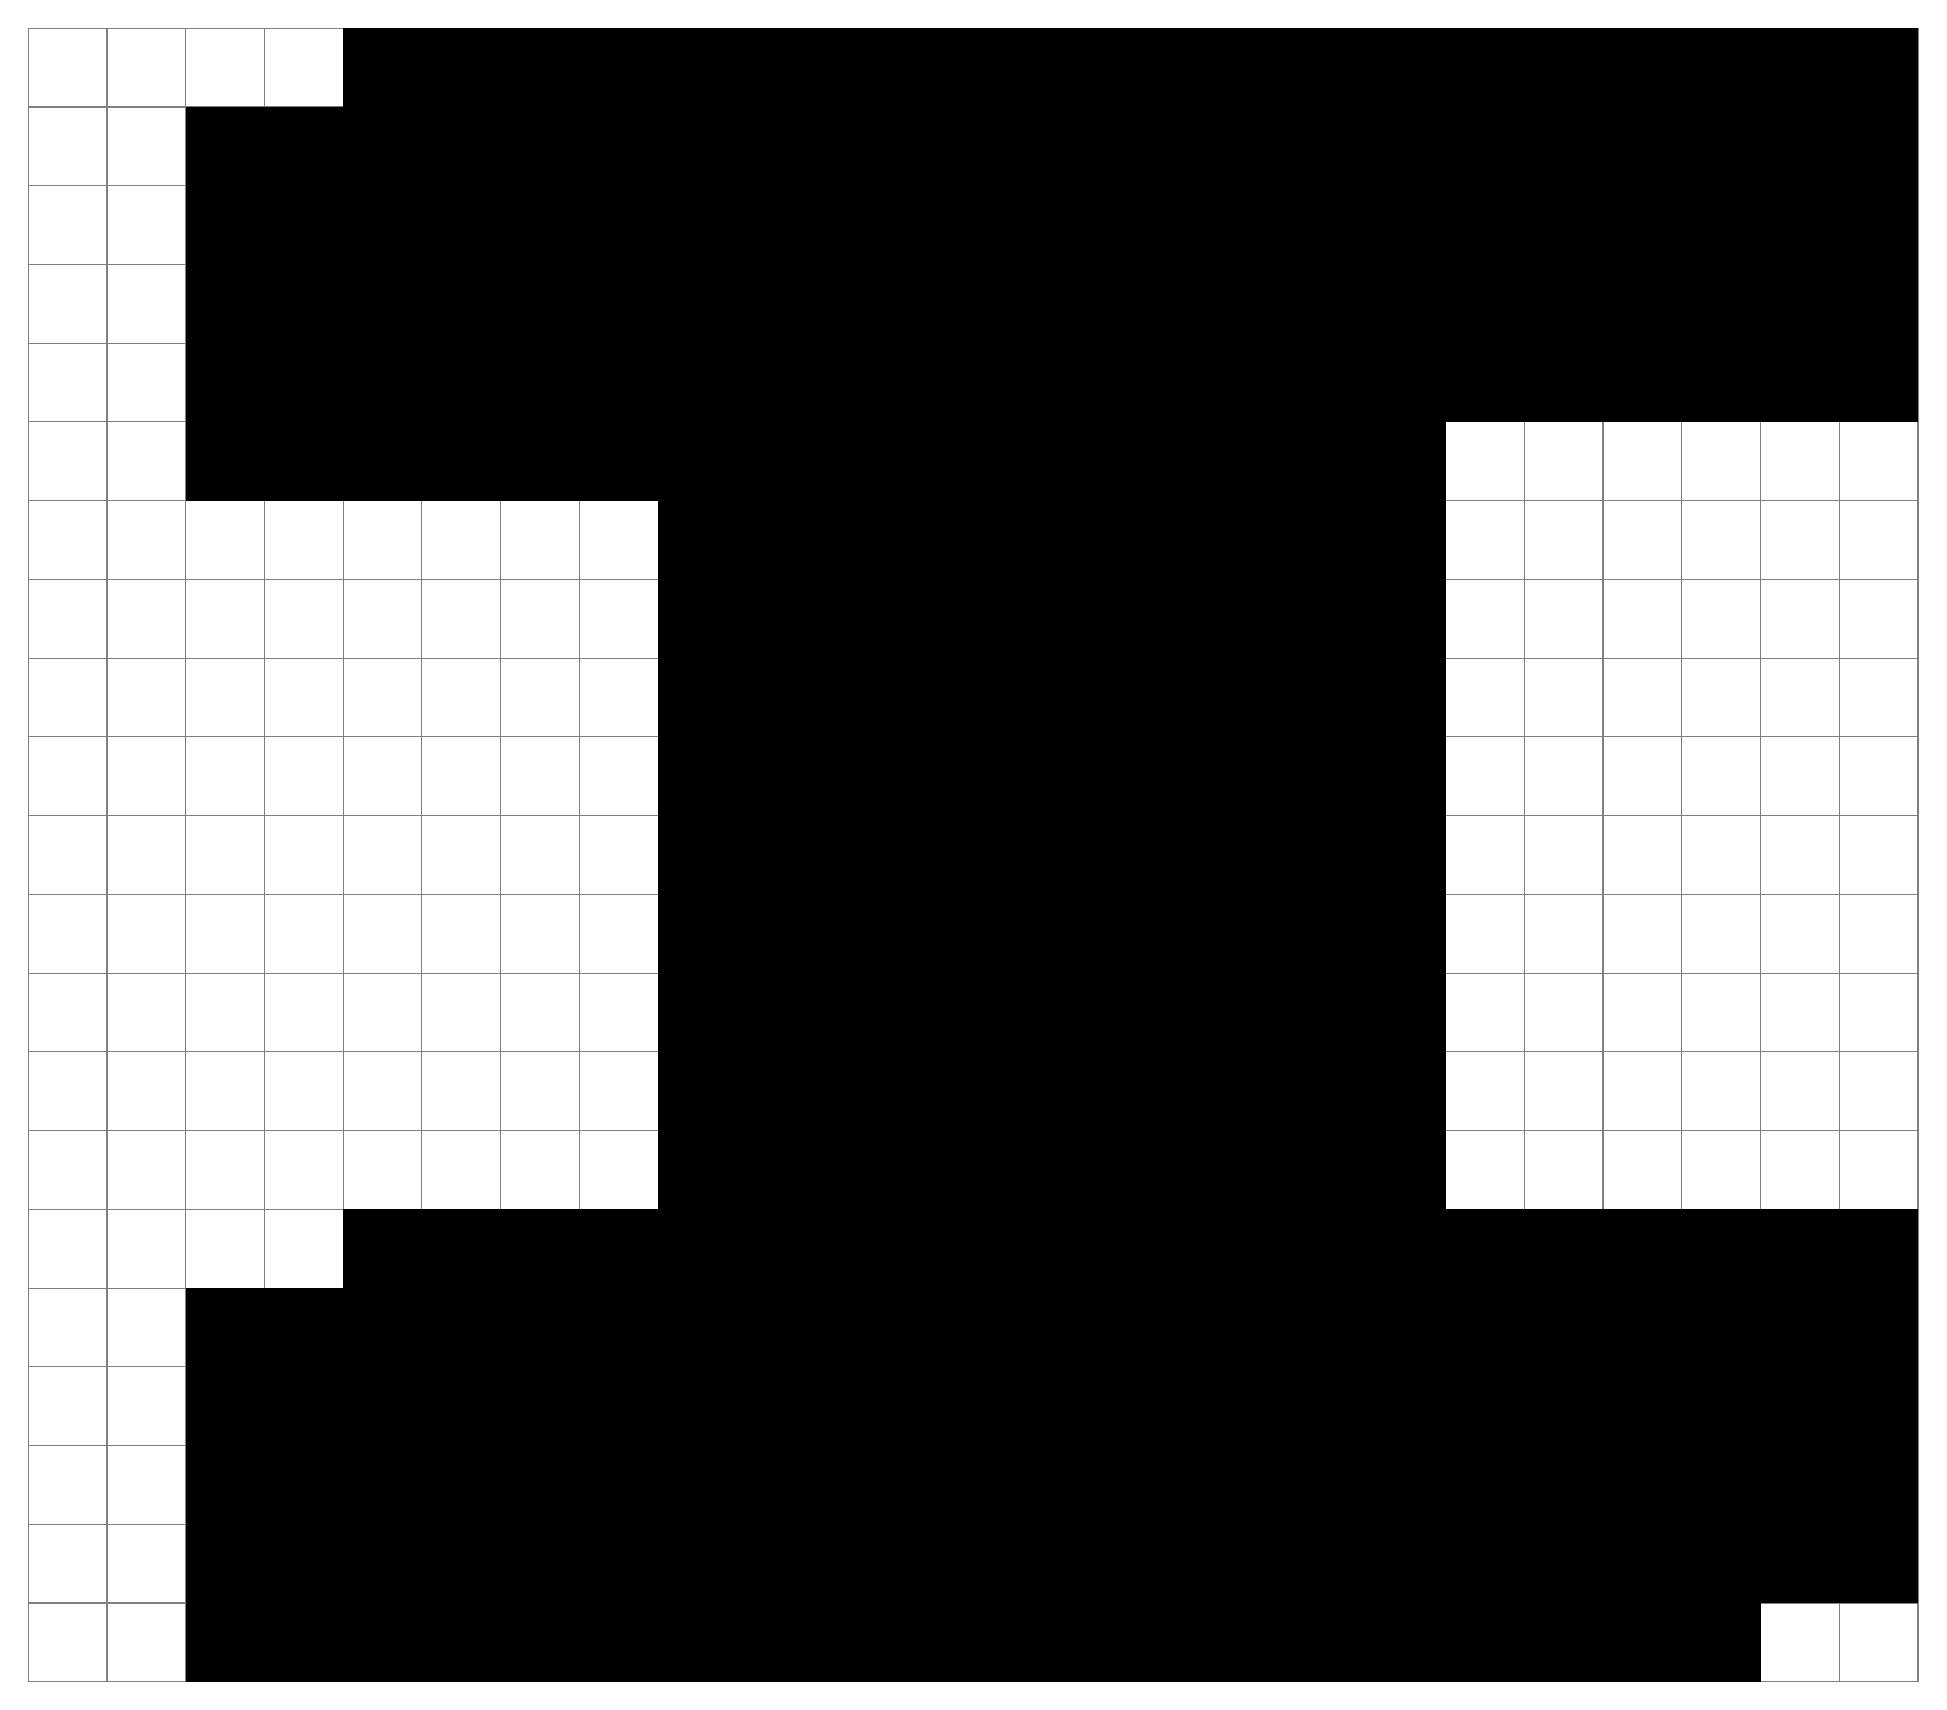
\begin{tikzpicture}

	\draw[step=1.0,gray,thin] (0,0) grid (24,21);
	\fill[\MULTICOLORTWO] (4,20) rectangle ++ (1,1);
	\fill[\MULTICOLORTWO] (5,20) rectangle ++ (1,1);
	\fill[\MULTICOLORTWO] (6,20) rectangle ++ (1,1);
	\fill[\MULTICOLORTWO] (7,20) rectangle ++ (1,1);
	\fill[\MULTICOLORTWO] (8,20) rectangle ++ (1,1);
	\fill[\MULTICOLORTWO] (9,20) rectangle ++ (1,1);
	\fill[\MULTICOLORTWO] (10,20) rectangle ++ (1,1);
	\fill[\MULTICOLORTWO] (11,20) rectangle ++ (1,1);
	\fill[\MULTICOLORTWO] (12,20) rectangle ++ (1,1);
	\fill[\MULTICOLORTWO] (13,20) rectangle ++ (1,1);
	\fill[\MULTICOLORTWO] (14,20) rectangle ++ (1,1);
	\fill[\MULTICOLORTWO] (15,20) rectangle ++ (1,1);
	\fill[\MULTICOLORTWO] (16,20) rectangle ++ (1,1);
	\fill[\MULTICOLORTWO] (17,20) rectangle ++ (1,1);
	\fill[\MULTICOLORTWO] (18,20) rectangle ++ (1,1);
	\fill[\MULTICOLORTWO] (19,20) rectangle ++ (1,1);
	\fill[\MULTICOLORTWO] (20,20) rectangle ++ (1,1);
	\fill[\MULTICOLORTWO] (21,20) rectangle ++ (1,1);
	\fill[\MULTICOLORTWO] (22,20) rectangle ++ (1,1);
	\fill[\MULTICOLORTWO] (23,20) rectangle ++ (1,1);
	\fill[\MULTICOLORONE] (2,19) rectangle ++ (1,1);
	\fill[\MULTICOLORONE] (3,19) rectangle ++ (1,1);
	\fill[\MULTICOLORTWO] (4,19) rectangle ++ (1,1);
	\fill[\MULTICOLORTWO] (5,19) rectangle ++ (1,1);
	\fill[\SPRITECOLOR] (6,19) rectangle ++ (1,1);
	\fill[\SPRITECOLOR] (7,19) rectangle ++ (1,1);
	\fill[\SPRITECOLOR] (8,19) rectangle ++ (1,1);
	\fill[\SPRITECOLOR] (9,19) rectangle ++ (1,1);
	\fill[\SPRITECOLOR] (10,19) rectangle ++ (1,1);
	\fill[\SPRITECOLOR] (11,19) rectangle ++ (1,1);
	\fill[\SPRITECOLOR] (12,19) rectangle ++ (1,1);
	\fill[\SPRITECOLOR] (13,19) rectangle ++ (1,1);
	\fill[\SPRITECOLOR] (14,19) rectangle ++ (1,1);
	\fill[\SPRITECOLOR] (15,19) rectangle ++ (1,1);
	\fill[\SPRITECOLOR] (16,19) rectangle ++ (1,1);
	\fill[\SPRITECOLOR] (17,19) rectangle ++ (1,1);
	\fill[\SPRITECOLOR] (18,19) rectangle ++ (1,1);
	\fill[\SPRITECOLOR] (19,19) rectangle ++ (1,1);
	\fill[\SPRITECOLOR] (20,19) rectangle ++ (1,1);
	\fill[\SPRITECOLOR] (21,19) rectangle ++ (1,1);
	\fill[\MULTICOLORTWO] (22,19) rectangle ++ (1,1);
	\fill[\MULTICOLORTWO] (23,19) rectangle ++ (1,1);
	\fill[\MULTICOLORONE] (2,18) rectangle ++ (1,1);
	\fill[\MULTICOLORONE] (3,18) rectangle ++ (1,1);
	\fill[\MULTICOLORTWO] (4,18) rectangle ++ (1,1);
	\fill[\MULTICOLORTWO] (5,18) rectangle ++ (1,1);
	\fill[\SPRITECOLOR] (6,18) rectangle ++ (1,1);
	\fill[\SPRITECOLOR] (7,18) rectangle ++ (1,1);
	\fill[\SPRITECOLOR] (8,18) rectangle ++ (1,1);
	\fill[\SPRITECOLOR] (9,18) rectangle ++ (1,1);
	\fill[\SPRITECOLOR] (10,18) rectangle ++ (1,1);
	\fill[\SPRITECOLOR] (11,18) rectangle ++ (1,1);
	\fill[\SPRITECOLOR] (12,18) rectangle ++ (1,1);
	\fill[\SPRITECOLOR] (13,18) rectangle ++ (1,1);
	\fill[\SPRITECOLOR] (14,18) rectangle ++ (1,1);
	\fill[\SPRITECOLOR] (15,18) rectangle ++ (1,1);
	\fill[\SPRITECOLOR] (16,18) rectangle ++ (1,1);
	\fill[\SPRITECOLOR] (17,18) rectangle ++ (1,1);
	\fill[\SPRITECOLOR] (18,18) rectangle ++ (1,1);
	\fill[\SPRITECOLOR] (19,18) rectangle ++ (1,1);
	\fill[\SPRITECOLOR] (20,18) rectangle ++ (1,1);
	\fill[\SPRITECOLOR] (21,18) rectangle ++ (1,1);
	\fill[\MULTICOLORTWO] (22,18) rectangle ++ (1,1);
	\fill[\MULTICOLORTWO] (23,18) rectangle ++ (1,1);
	\fill[\MULTICOLORONE] (2,17) rectangle ++ (1,1);
	\fill[\MULTICOLORONE] (3,17) rectangle ++ (1,1);
	\fill[\MULTICOLORTWO] (4,17) rectangle ++ (1,1);
	\fill[\MULTICOLORTWO] (5,17) rectangle ++ (1,1);
	\fill[\SPRITECOLOR] (6,17) rectangle ++ (1,1);
	\fill[\SPRITECOLOR] (7,17) rectangle ++ (1,1);
	\fill[\SPRITECOLOR] (8,17) rectangle ++ (1,1);
	\fill[\SPRITECOLOR] (9,17) rectangle ++ (1,1);
	\fill[\SPRITECOLOR] (10,17) rectangle ++ (1,1);
	\fill[\SPRITECOLOR] (11,17) rectangle ++ (1,1);
	\fill[\SPRITECOLOR] (12,17) rectangle ++ (1,1);
	\fill[\SPRITECOLOR] (13,17) rectangle ++ (1,1);
	\fill[\SPRITECOLOR] (14,17) rectangle ++ (1,1);
	\fill[\SPRITECOLOR] (15,17) rectangle ++ (1,1);
	\fill[\SPRITECOLOR] (16,17) rectangle ++ (1,1);
	\fill[\SPRITECOLOR] (17,17) rectangle ++ (1,1);
	\fill[\SPRITECOLOR] (18,17) rectangle ++ (1,1);
	\fill[\SPRITECOLOR] (19,17) rectangle ++ (1,1);
	\fill[\SPRITECOLOR] (20,17) rectangle ++ (1,1);
	\fill[\SPRITECOLOR] (21,17) rectangle ++ (1,1);
	\fill[\MULTICOLORTWO] (22,17) rectangle ++ (1,1);
	\fill[\MULTICOLORTWO] (23,17) rectangle ++ (1,1);
	\fill[\MULTICOLORONE] (2,16) rectangle ++ (1,1);
	\fill[\MULTICOLORONE] (3,16) rectangle ++ (1,1);
	\fill[\MULTICOLORTWO] (4,16) rectangle ++ (1,1);
	\fill[\MULTICOLORTWO] (5,16) rectangle ++ (1,1);
	\fill[\MULTICOLORTWO] (6,16) rectangle ++ (1,1);
	\fill[\MULTICOLORTWO] (7,16) rectangle ++ (1,1);
	\fill[\MULTICOLORTWO] (8,16) rectangle ++ (1,1);
	\fill[\MULTICOLORTWO] (9,16) rectangle ++ (1,1);
	\fill[\MULTICOLORTWO] (10,16) rectangle ++ (1,1);
	\fill[\MULTICOLORTWO] (11,16) rectangle ++ (1,1);
	\fill[\SPRITECOLOR] (12,16) rectangle ++ (1,1);
	\fill[\SPRITECOLOR] (13,16) rectangle ++ (1,1);
	\fill[\SPRITECOLOR] (14,16) rectangle ++ (1,1);
	\fill[\SPRITECOLOR] (15,16) rectangle ++ (1,1);
	\fill[\MULTICOLORTWO] (16,16) rectangle ++ (1,1);
	\fill[\MULTICOLORTWO] (17,16) rectangle ++ (1,1);
	\fill[\MULTICOLORTWO] (18,16) rectangle ++ (1,1);
	\fill[\MULTICOLORTWO] (19,16) rectangle ++ (1,1);
	\fill[\MULTICOLORTWO] (20,16) rectangle ++ (1,1);
	\fill[\MULTICOLORTWO] (21,16) rectangle ++ (1,1);
	\fill[\MULTICOLORTWO] (22,16) rectangle ++ (1,1);
	\fill[\MULTICOLORTWO] (23,16) rectangle ++ (1,1);
	\fill[\MULTICOLORONE] (2,15) rectangle ++ (1,1);
	\fill[\MULTICOLORONE] (3,15) rectangle ++ (1,1);
	\fill[\MULTICOLORONE] (4,15) rectangle ++ (1,1);
	\fill[\MULTICOLORONE] (5,15) rectangle ++ (1,1);
	\fill[\MULTICOLORONE] (6,15) rectangle ++ (1,1);
	\fill[\MULTICOLORONE] (7,15) rectangle ++ (1,1);
	\fill[\MULTICOLORONE] (8,15) rectangle ++ (1,1);
	\fill[\MULTICOLORONE] (9,15) rectangle ++ (1,1);
	\fill[\MULTICOLORTWO] (10,15) rectangle ++ (1,1);
	\fill[\MULTICOLORTWO] (11,15) rectangle ++ (1,1);
	\fill[\SPRITECOLOR] (12,15) rectangle ++ (1,1);
	\fill[\SPRITECOLOR] (13,15) rectangle ++ (1,1);
	\fill[\SPRITECOLOR] (14,15) rectangle ++ (1,1);
	\fill[\SPRITECOLOR] (15,15) rectangle ++ (1,1);
	\fill[\MULTICOLORTWO] (16,15) rectangle ++ (1,1);
	\fill[\MULTICOLORTWO] (17,15) rectangle ++ (1,1);
	\fill[\MULTICOLORONE] (8,14) rectangle ++ (1,1);
	\fill[\MULTICOLORONE] (9,14) rectangle ++ (1,1);
	\fill[\MULTICOLORTWO] (10,14) rectangle ++ (1,1);
	\fill[\MULTICOLORTWO] (11,14) rectangle ++ (1,1);
	\fill[\SPRITECOLOR] (12,14) rectangle ++ (1,1);
	\fill[\SPRITECOLOR] (13,14) rectangle ++ (1,1);
	\fill[\SPRITECOLOR] (14,14) rectangle ++ (1,1);
	\fill[\SPRITECOLOR] (15,14) rectangle ++ (1,1);
	\fill[\MULTICOLORTWO] (16,14) rectangle ++ (1,1);
	\fill[\MULTICOLORTWO] (17,14) rectangle ++ (1,1);
	\fill[\MULTICOLORONE] (8,13) rectangle ++ (1,1);
	\fill[\MULTICOLORONE] (9,13) rectangle ++ (1,1);
	\fill[\MULTICOLORTWO] (10,13) rectangle ++ (1,1);
	\fill[\MULTICOLORTWO] (11,13) rectangle ++ (1,1);
	\fill[\SPRITECOLOR] (12,13) rectangle ++ (1,1);
	\fill[\SPRITECOLOR] (13,13) rectangle ++ (1,1);
	\fill[\SPRITECOLOR] (14,13) rectangle ++ (1,1);
	\fill[\SPRITECOLOR] (15,13) rectangle ++ (1,1);
	\fill[\MULTICOLORTWO] (16,13) rectangle ++ (1,1);
	\fill[\MULTICOLORTWO] (17,13) rectangle ++ (1,1);
	\fill[\MULTICOLORONE] (8,12) rectangle ++ (1,1);
	\fill[\MULTICOLORONE] (9,12) rectangle ++ (1,1);
	\fill[\MULTICOLORTWO] (10,12) rectangle ++ (1,1);
	\fill[\MULTICOLORTWO] (11,12) rectangle ++ (1,1);
	\fill[\SPRITECOLOR] (12,12) rectangle ++ (1,1);
	\fill[\SPRITECOLOR] (13,12) rectangle ++ (1,1);
	\fill[\SPRITECOLOR] (14,12) rectangle ++ (1,1);
	\fill[\SPRITECOLOR] (15,12) rectangle ++ (1,1);
	\fill[\MULTICOLORTWO] (16,12) rectangle ++ (1,1);
	\fill[\MULTICOLORTWO] (17,12) rectangle ++ (1,1);
	\fill[\MULTICOLORONE] (8,11) rectangle ++ (1,1);
	\fill[\MULTICOLORONE] (9,11) rectangle ++ (1,1);
	\fill[\MULTICOLORTWO] (10,11) rectangle ++ (1,1);
	\fill[\MULTICOLORTWO] (11,11) rectangle ++ (1,1);
	\fill[\SPRITECOLOR] (12,11) rectangle ++ (1,1);
	\fill[\SPRITECOLOR] (13,11) rectangle ++ (1,1);
	\fill[\SPRITECOLOR] (14,11) rectangle ++ (1,1);
	\fill[\SPRITECOLOR] (15,11) rectangle ++ (1,1);
	\fill[\MULTICOLORTWO] (16,11) rectangle ++ (1,1);
	\fill[\MULTICOLORTWO] (17,11) rectangle ++ (1,1);
	\fill[\MULTICOLORONE] (8,10) rectangle ++ (1,1);
	\fill[\MULTICOLORONE] (9,10) rectangle ++ (1,1);
	\fill[\MULTICOLORTWO] (10,10) rectangle ++ (1,1);
	\fill[\MULTICOLORTWO] (11,10) rectangle ++ (1,1);
	\fill[\SPRITECOLOR] (12,10) rectangle ++ (1,1);
	\fill[\SPRITECOLOR] (13,10) rectangle ++ (1,1);
	\fill[\SPRITECOLOR] (14,10) rectangle ++ (1,1);
	\fill[\SPRITECOLOR] (15,10) rectangle ++ (1,1);
	\fill[\MULTICOLORTWO] (16,10) rectangle ++ (1,1);
	\fill[\MULTICOLORTWO] (17,10) rectangle ++ (1,1);
	\fill[\MULTICOLORONE] (8,9) rectangle ++ (1,1);
	\fill[\MULTICOLORONE] (9,9) rectangle ++ (1,1);
	\fill[\MULTICOLORTWO] (10,9) rectangle ++ (1,1);
	\fill[\MULTICOLORTWO] (11,9) rectangle ++ (1,1);
	\fill[\SPRITECOLOR] (12,9) rectangle ++ (1,1);
	\fill[\SPRITECOLOR] (13,9) rectangle ++ (1,1);
	\fill[\SPRITECOLOR] (14,9) rectangle ++ (1,1);
	\fill[\SPRITECOLOR] (15,9) rectangle ++ (1,1);
	\fill[\MULTICOLORTWO] (16,9) rectangle ++ (1,1);
	\fill[\MULTICOLORTWO] (17,9) rectangle ++ (1,1);
	\fill[\MULTICOLORONE] (8,8) rectangle ++ (1,1);
	\fill[\MULTICOLORONE] (9,8) rectangle ++ (1,1);
	\fill[\MULTICOLORTWO] (10,8) rectangle ++ (1,1);
	\fill[\MULTICOLORTWO] (11,8) rectangle ++ (1,1);
	\fill[\SPRITECOLOR] (12,8) rectangle ++ (1,1);
	\fill[\SPRITECOLOR] (13,8) rectangle ++ (1,1);
	\fill[\SPRITECOLOR] (14,8) rectangle ++ (1,1);
	\fill[\SPRITECOLOR] (15,8) rectangle ++ (1,1);
	\fill[\MULTICOLORTWO] (16,8) rectangle ++ (1,1);
	\fill[\MULTICOLORTWO] (17,8) rectangle ++ (1,1);
	\fill[\MULTICOLORONE] (8,7) rectangle ++ (1,1);
	\fill[\MULTICOLORONE] (9,7) rectangle ++ (1,1);
	\fill[\MULTICOLORTWO] (10,7) rectangle ++ (1,1);
	\fill[\MULTICOLORTWO] (11,7) rectangle ++ (1,1);
	\fill[\SPRITECOLOR] (12,7) rectangle ++ (1,1);
	\fill[\SPRITECOLOR] (13,7) rectangle ++ (1,1);
	\fill[\SPRITECOLOR] (14,7) rectangle ++ (1,1);
	\fill[\SPRITECOLOR] (15,7) rectangle ++ (1,1);
	\fill[\MULTICOLORTWO] (16,7) rectangle ++ (1,1);
	\fill[\MULTICOLORTWO] (17,7) rectangle ++ (1,1);
	\fill[\MULTICOLORONE] (8,6) rectangle ++ (1,1);
	\fill[\MULTICOLORONE] (9,6) rectangle ++ (1,1);
	\fill[\MULTICOLORTWO] (10,6) rectangle ++ (1,1);
	\fill[\MULTICOLORTWO] (11,6) rectangle ++ (1,1);
	\fill[\SPRITECOLOR] (12,6) rectangle ++ (1,1);
	\fill[\SPRITECOLOR] (13,6) rectangle ++ (1,1);
	\fill[\SPRITECOLOR] (14,6) rectangle ++ (1,1);
	\fill[\SPRITECOLOR] (15,6) rectangle ++ (1,1);
	\fill[\MULTICOLORTWO] (16,6) rectangle ++ (1,1);
	\fill[\MULTICOLORTWO] (17,6) rectangle ++ (1,1);
	\fill[\MULTICOLORTWO] (4,5) rectangle ++ (1,1);
	\fill[\MULTICOLORTWO] (5,5) rectangle ++ (1,1);
	\fill[\MULTICOLORTWO] (6,5) rectangle ++ (1,1);
	\fill[\MULTICOLORTWO] (7,5) rectangle ++ (1,1);
	\fill[\MULTICOLORTWO] (8,5) rectangle ++ (1,1);
	\fill[\MULTICOLORTWO] (9,5) rectangle ++ (1,1);
	\fill[\MULTICOLORTWO] (10,5) rectangle ++ (1,1);
	\fill[\MULTICOLORTWO] (11,5) rectangle ++ (1,1);
	\fill[\SPRITECOLOR] (12,5) rectangle ++ (1,1);
	\fill[\SPRITECOLOR] (13,5) rectangle ++ (1,1);
	\fill[\SPRITECOLOR] (14,5) rectangle ++ (1,1);
	\fill[\SPRITECOLOR] (15,5) rectangle ++ (1,1);
	\fill[\MULTICOLORTWO] (16,5) rectangle ++ (1,1);
	\fill[\MULTICOLORTWO] (17,5) rectangle ++ (1,1);
	\fill[\MULTICOLORTWO] (18,5) rectangle ++ (1,1);
	\fill[\MULTICOLORTWO] (19,5) rectangle ++ (1,1);
	\fill[\MULTICOLORTWO] (20,5) rectangle ++ (1,1);
	\fill[\MULTICOLORTWO] (21,5) rectangle ++ (1,1);
	\fill[\MULTICOLORTWO] (22,5) rectangle ++ (1,1);
	\fill[\MULTICOLORTWO] (23,5) rectangle ++ (1,1);
	\fill[\MULTICOLORONE] (2,4) rectangle ++ (1,1);
	\fill[\MULTICOLORONE] (3,4) rectangle ++ (1,1);
	\fill[\MULTICOLORTWO] (4,4) rectangle ++ (1,1);
	\fill[\MULTICOLORTWO] (5,4) rectangle ++ (1,1);
	\fill[\SPRITECOLOR] (6,4) rectangle ++ (1,1);
	\fill[\SPRITECOLOR] (7,4) rectangle ++ (1,1);
	\fill[\SPRITECOLOR] (8,4) rectangle ++ (1,1);
	\fill[\SPRITECOLOR] (9,4) rectangle ++ (1,1);
	\fill[\SPRITECOLOR] (10,4) rectangle ++ (1,1);
	\fill[\SPRITECOLOR] (11,4) rectangle ++ (1,1);
	\fill[\SPRITECOLOR] (12,4) rectangle ++ (1,1);
	\fill[\SPRITECOLOR] (13,4) rectangle ++ (1,1);
	\fill[\SPRITECOLOR] (14,4) rectangle ++ (1,1);
	\fill[\SPRITECOLOR] (15,4) rectangle ++ (1,1);
	\fill[\SPRITECOLOR] (16,4) rectangle ++ (1,1);
	\fill[\SPRITECOLOR] (17,4) rectangle ++ (1,1);
	\fill[\SPRITECOLOR] (18,4) rectangle ++ (1,1);
	\fill[\SPRITECOLOR] (19,4) rectangle ++ (1,1);
	\fill[\SPRITECOLOR] (20,4) rectangle ++ (1,1);
	\fill[\SPRITECOLOR] (21,4) rectangle ++ (1,1);
	\fill[\MULTICOLORTWO] (22,4) rectangle ++ (1,1);
	\fill[\MULTICOLORTWO] (23,4) rectangle ++ (1,1);
	\fill[\MULTICOLORONE] (2,3) rectangle ++ (1,1);
	\fill[\MULTICOLORONE] (3,3) rectangle ++ (1,1);
	\fill[\MULTICOLORTWO] (4,3) rectangle ++ (1,1);
	\fill[\MULTICOLORTWO] (5,3) rectangle ++ (1,1);
	\fill[\SPRITECOLOR] (6,3) rectangle ++ (1,1);
	\fill[\SPRITECOLOR] (7,3) rectangle ++ (1,1);
	\fill[\SPRITECOLOR] (8,3) rectangle ++ (1,1);
	\fill[\SPRITECOLOR] (9,3) rectangle ++ (1,1);
	\fill[\SPRITECOLOR] (10,3) rectangle ++ (1,1);
	\fill[\SPRITECOLOR] (11,3) rectangle ++ (1,1);
	\fill[\SPRITECOLOR] (12,3) rectangle ++ (1,1);
	\fill[\SPRITECOLOR] (13,3) rectangle ++ (1,1);
	\fill[\SPRITECOLOR] (14,3) rectangle ++ (1,1);
	\fill[\SPRITECOLOR] (15,3) rectangle ++ (1,1);
	\fill[\SPRITECOLOR] (16,3) rectangle ++ (1,1);
	\fill[\SPRITECOLOR] (17,3) rectangle ++ (1,1);
	\fill[\SPRITECOLOR] (18,3) rectangle ++ (1,1);
	\fill[\SPRITECOLOR] (19,3) rectangle ++ (1,1);
	\fill[\SPRITECOLOR] (20,3) rectangle ++ (1,1);
	\fill[\SPRITECOLOR] (21,3) rectangle ++ (1,1);
	\fill[\MULTICOLORTWO] (22,3) rectangle ++ (1,1);
	\fill[\MULTICOLORTWO] (23,3) rectangle ++ (1,1);
	\fill[\MULTICOLORONE] (2,2) rectangle ++ (1,1);
	\fill[\MULTICOLORONE] (3,2) rectangle ++ (1,1);
	\fill[\MULTICOLORTWO] (4,2) rectangle ++ (1,1);
	\fill[\MULTICOLORTWO] (5,2) rectangle ++ (1,1);
	\fill[\SPRITECOLOR] (6,2) rectangle ++ (1,1);
	\fill[\SPRITECOLOR] (7,2) rectangle ++ (1,1);
	\fill[\SPRITECOLOR] (8,2) rectangle ++ (1,1);
	\fill[\SPRITECOLOR] (9,2) rectangle ++ (1,1);
	\fill[\SPRITECOLOR] (10,2) rectangle ++ (1,1);
	\fill[\SPRITECOLOR] (11,2) rectangle ++ (1,1);
	\fill[\SPRITECOLOR] (12,2) rectangle ++ (1,1);
	\fill[\SPRITECOLOR] (13,2) rectangle ++ (1,1);
	\fill[\SPRITECOLOR] (14,2) rectangle ++ (1,1);
	\fill[\SPRITECOLOR] (15,2) rectangle ++ (1,1);
	\fill[\SPRITECOLOR] (16,2) rectangle ++ (1,1);
	\fill[\SPRITECOLOR] (17,2) rectangle ++ (1,1);
	\fill[\SPRITECOLOR] (18,2) rectangle ++ (1,1);
	\fill[\SPRITECOLOR] (19,2) rectangle ++ (1,1);
	\fill[\SPRITECOLOR] (20,2) rectangle ++ (1,1);
	\fill[\SPRITECOLOR] (21,2) rectangle ++ (1,1);
	\fill[\MULTICOLORTWO] (22,2) rectangle ++ (1,1);
	\fill[\MULTICOLORTWO] (23,2) rectangle ++ (1,1);
	\fill[\MULTICOLORONE] (2,1) rectangle ++ (1,1);
	\fill[\MULTICOLORONE] (3,1) rectangle ++ (1,1);
	\fill[\MULTICOLORTWO] (4,1) rectangle ++ (1,1);
	\fill[\MULTICOLORTWO] (5,1) rectangle ++ (1,1);
	\fill[\MULTICOLORTWO] (6,1) rectangle ++ (1,1);
	\fill[\MULTICOLORTWO] (7,1) rectangle ++ (1,1);
	\fill[\MULTICOLORTWO] (8,1) rectangle ++ (1,1);
	\fill[\MULTICOLORTWO] (9,1) rectangle ++ (1,1);
	\fill[\MULTICOLORTWO] (10,1) rectangle ++ (1,1);
	\fill[\MULTICOLORTWO] (11,1) rectangle ++ (1,1);
	\fill[\MULTICOLORTWO] (12,1) rectangle ++ (1,1);
	\fill[\MULTICOLORTWO] (13,1) rectangle ++ (1,1);
	\fill[\MULTICOLORTWO] (14,1) rectangle ++ (1,1);
	\fill[\MULTICOLORTWO] (15,1) rectangle ++ (1,1);
	\fill[\MULTICOLORTWO] (16,1) rectangle ++ (1,1);
	\fill[\MULTICOLORTWO] (17,1) rectangle ++ (1,1);
	\fill[\MULTICOLORTWO] (18,1) rectangle ++ (1,1);
	\fill[\MULTICOLORTWO] (19,1) rectangle ++ (1,1);
	\fill[\MULTICOLORTWO] (20,1) rectangle ++ (1,1);
	\fill[\MULTICOLORTWO] (21,1) rectangle ++ (1,1);
	\fill[\MULTICOLORTWO] (22,1) rectangle ++ (1,1);
	\fill[\MULTICOLORTWO] (23,1) rectangle ++ (1,1);
	\fill[\MULTICOLORONE] (2,0) rectangle ++ (1,1);
	\fill[\MULTICOLORONE] (3,0) rectangle ++ (1,1);
	\fill[\MULTICOLORONE] (4,0) rectangle ++ (1,1);
	\fill[\MULTICOLORONE] (5,0) rectangle ++ (1,1);
	\fill[\MULTICOLORONE] (6,0) rectangle ++ (1,1);
	\fill[\MULTICOLORONE] (7,0) rectangle ++ (1,1);
	\fill[\MULTICOLORONE] (8,0) rectangle ++ (1,1);
	\fill[\MULTICOLORONE] (9,0) rectangle ++ (1,1);
	\fill[\MULTICOLORONE] (10,0) rectangle ++ (1,1);
	\fill[\MULTICOLORONE] (11,0) rectangle ++ (1,1);
	\fill[\MULTICOLORONE] (12,0) rectangle ++ (1,1);
	\fill[\MULTICOLORONE] (13,0) rectangle ++ (1,1);
	\fill[\MULTICOLORONE] (14,0) rectangle ++ (1,1);
	\fill[\MULTICOLORONE] (15,0) rectangle ++ (1,1);
	\fill[\MULTICOLORONE] (16,0) rectangle ++ (1,1);
	\fill[\MULTICOLORONE] (17,0) rectangle ++ (1,1);
	\fill[\MULTICOLORONE] (18,0) rectangle ++ (1,1);
	\fill[\MULTICOLORONE] (19,0) rectangle ++ (1,1);
	\fill[\MULTICOLORONE] (20,0) rectangle ++ (1,1);
	\fill[\MULTICOLORONE] (21,0) rectangle ++ (1,1);

      \end{tikzpicture}
    \end{adjustbox}
  }\caption{BIG\_I}
\end{figure}

	\end{subfigure}
} &
\makecell[l]{
	\begin{subfigure}{0.3\textwidth}
    \def\MULTICOLORONE{gray}
    \def\MULTICOLORTWO{black}
    \def\SPRITECOLOR{purple}
		
\begin{figure}[H]
  {
    \setlength{\tabcolsep}{3.0pt}
    \setlength\cmidrulewidth{\heavyrulewidth} % Make cmidrule = 
    \begin{adjustbox}{width=3cm,center}
      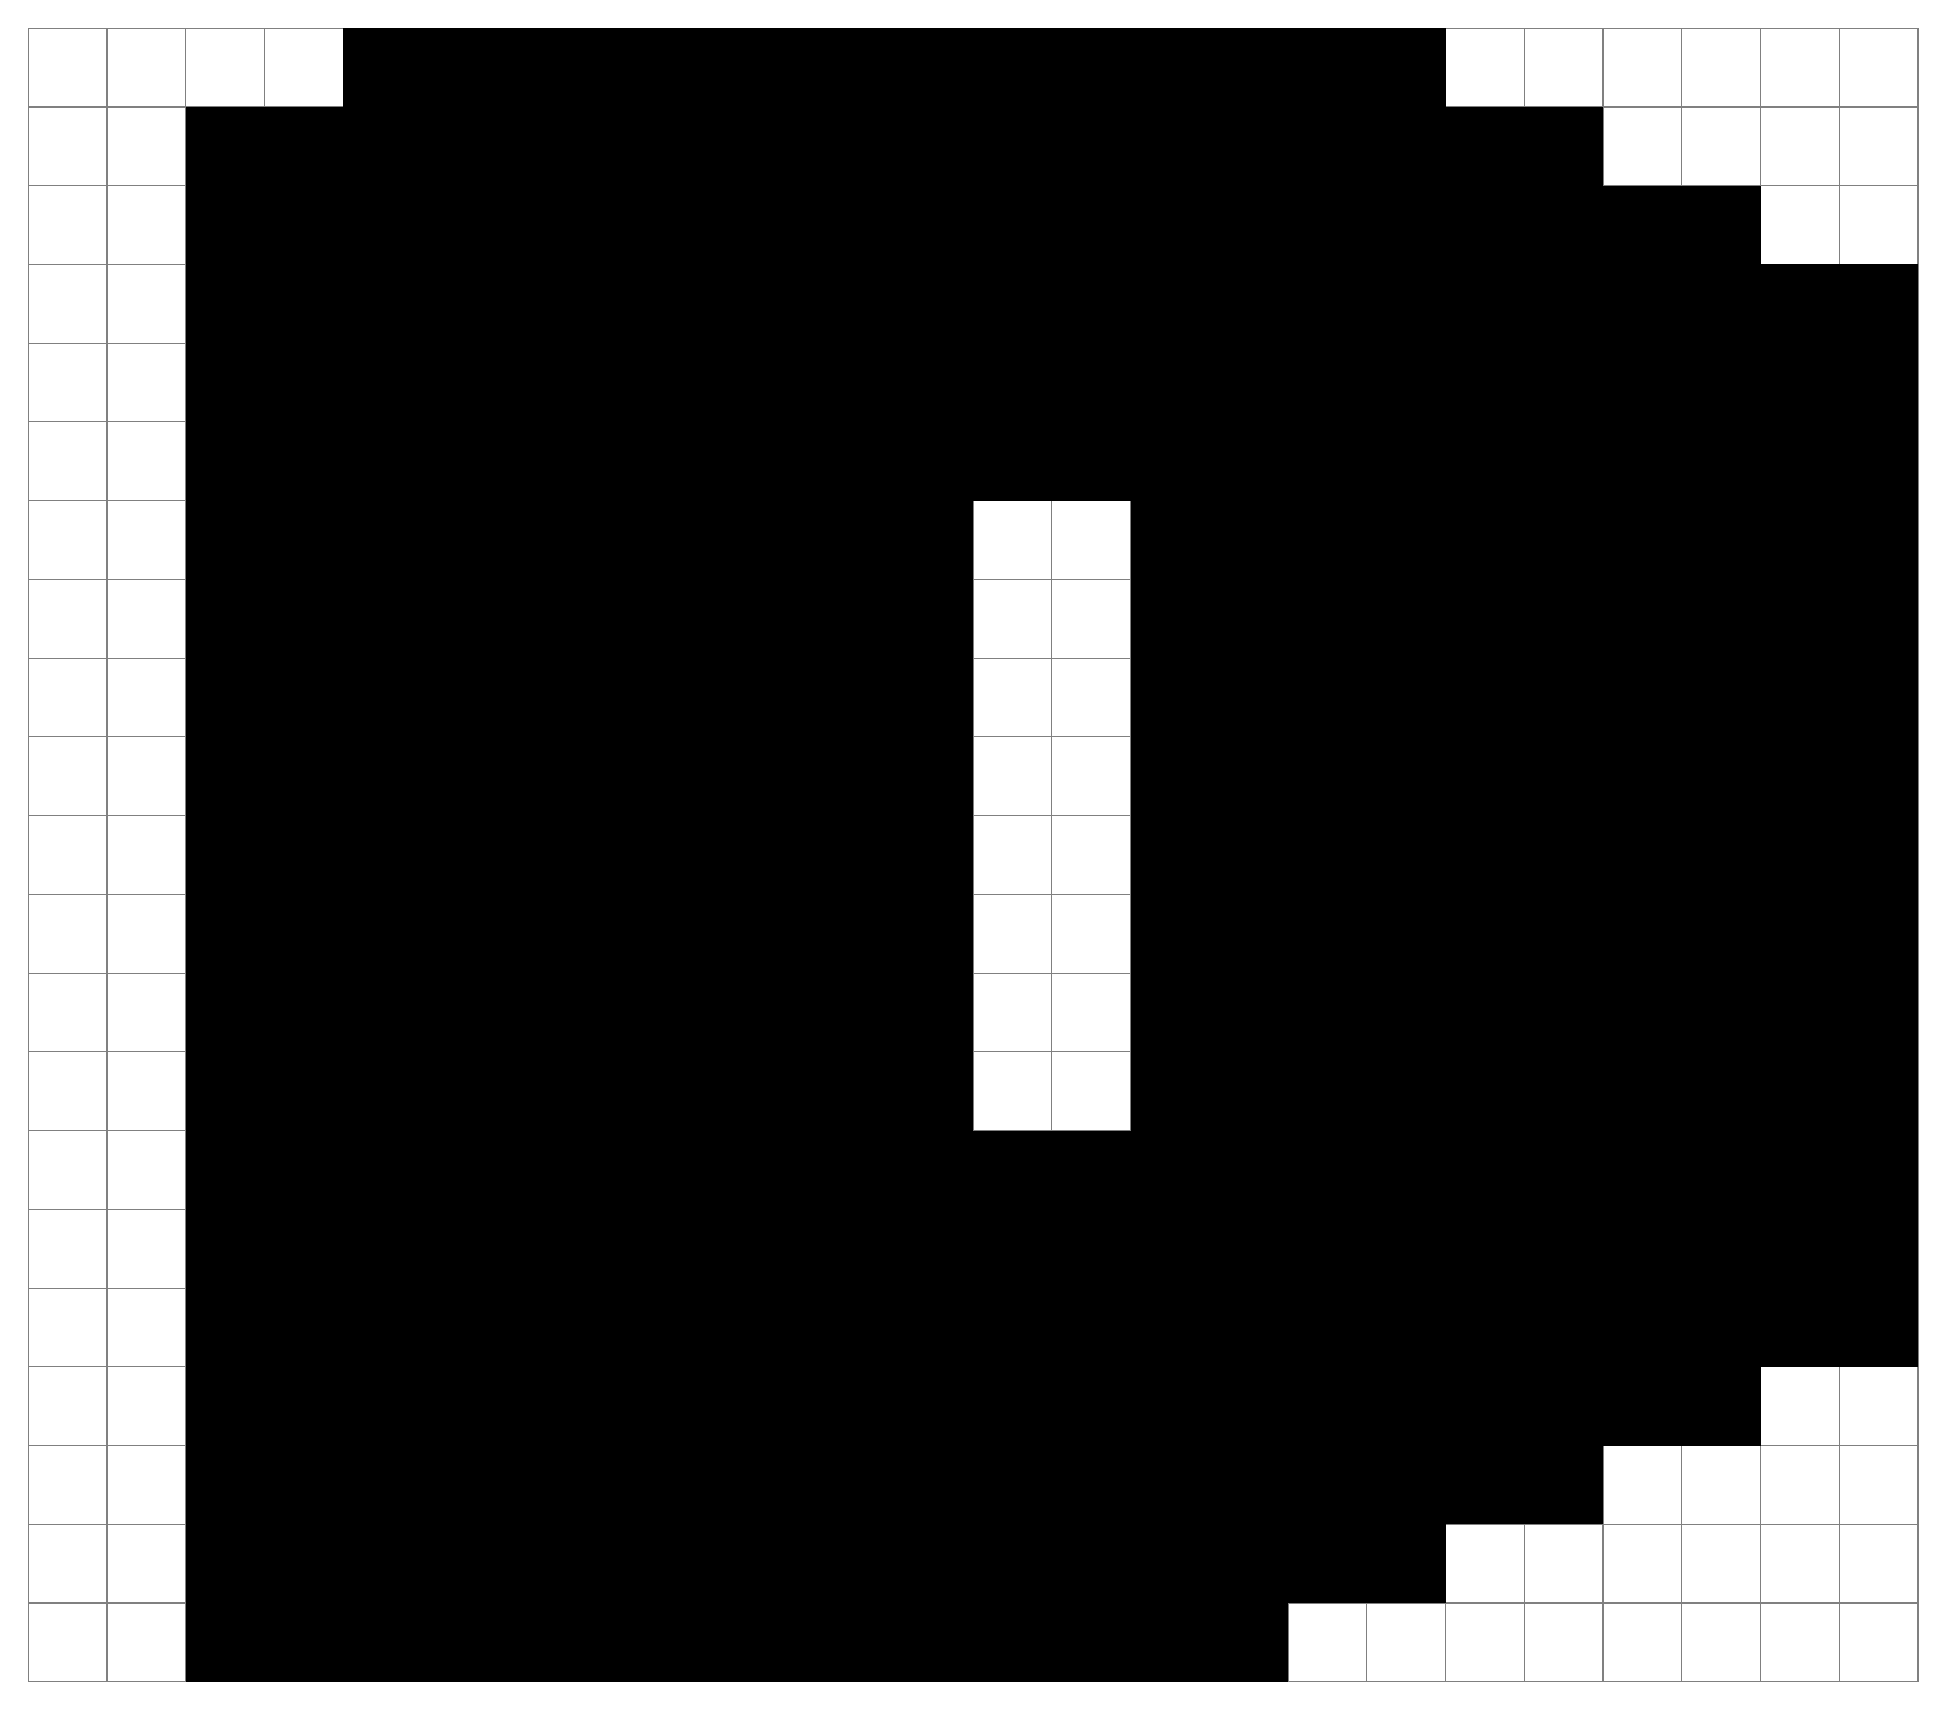
\begin{tikzpicture}

	\draw[step=1.0,gray,thin] (0,0) grid (24,21);
	\fill[\MULTICOLORTWO] (4,20) rectangle ++ (1,1);
	\fill[\MULTICOLORTWO] (5,20) rectangle ++ (1,1);
	\fill[\MULTICOLORTWO] (6,20) rectangle ++ (1,1);
	\fill[\MULTICOLORTWO] (7,20) rectangle ++ (1,1);
	\fill[\MULTICOLORTWO] (8,20) rectangle ++ (1,1);
	\fill[\MULTICOLORTWO] (9,20) rectangle ++ (1,1);
	\fill[\MULTICOLORTWO] (10,20) rectangle ++ (1,1);
	\fill[\MULTICOLORTWO] (11,20) rectangle ++ (1,1);
	\fill[\MULTICOLORTWO] (12,20) rectangle ++ (1,1);
	\fill[\MULTICOLORTWO] (13,20) rectangle ++ (1,1);
	\fill[\MULTICOLORTWO] (14,20) rectangle ++ (1,1);
	\fill[\MULTICOLORTWO] (15,20) rectangle ++ (1,1);
	\fill[\MULTICOLORTWO] (16,20) rectangle ++ (1,1);
	\fill[\MULTICOLORTWO] (17,20) rectangle ++ (1,1);
	\fill[\MULTICOLORONE] (2,19) rectangle ++ (1,1);
	\fill[\MULTICOLORONE] (3,19) rectangle ++ (1,1);
	\fill[\MULTICOLORTWO] (4,19) rectangle ++ (1,1);
	\fill[\MULTICOLORTWO] (5,19) rectangle ++ (1,1);
	\fill[\SPRITECOLOR] (6,19) rectangle ++ (1,1);
	\fill[\SPRITECOLOR] (7,19) rectangle ++ (1,1);
	\fill[\SPRITECOLOR] (8,19) rectangle ++ (1,1);
	\fill[\SPRITECOLOR] (9,19) rectangle ++ (1,1);
	\fill[\SPRITECOLOR] (10,19) rectangle ++ (1,1);
	\fill[\SPRITECOLOR] (11,19) rectangle ++ (1,1);
	\fill[\SPRITECOLOR] (12,19) rectangle ++ (1,1);
	\fill[\SPRITECOLOR] (13,19) rectangle ++ (1,1);
	\fill[\SPRITECOLOR] (14,19) rectangle ++ (1,1);
	\fill[\SPRITECOLOR] (15,19) rectangle ++ (1,1);
	\fill[\SPRITECOLOR] (16,19) rectangle ++ (1,1);
	\fill[\SPRITECOLOR] (17,19) rectangle ++ (1,1);
	\fill[\MULTICOLORTWO] (18,19) rectangle ++ (1,1);
	\fill[\MULTICOLORTWO] (19,19) rectangle ++ (1,1);
	\fill[\MULTICOLORONE] (2,18) rectangle ++ (1,1);
	\fill[\MULTICOLORONE] (3,18) rectangle ++ (1,1);
	\fill[\MULTICOLORTWO] (4,18) rectangle ++ (1,1);
	\fill[\MULTICOLORTWO] (5,18) rectangle ++ (1,1);
	\fill[\SPRITECOLOR] (6,18) rectangle ++ (1,1);
	\fill[\SPRITECOLOR] (7,18) rectangle ++ (1,1);
	\fill[\SPRITECOLOR] (8,18) rectangle ++ (1,1);
	\fill[\SPRITECOLOR] (9,18) rectangle ++ (1,1);
	\fill[\SPRITECOLOR] (10,18) rectangle ++ (1,1);
	\fill[\SPRITECOLOR] (11,18) rectangle ++ (1,1);
	\fill[\SPRITECOLOR] (12,18) rectangle ++ (1,1);
	\fill[\SPRITECOLOR] (13,18) rectangle ++ (1,1);
	\fill[\SPRITECOLOR] (14,18) rectangle ++ (1,1);
	\fill[\SPRITECOLOR] (15,18) rectangle ++ (1,1);
	\fill[\SPRITECOLOR] (16,18) rectangle ++ (1,1);
	\fill[\SPRITECOLOR] (17,18) rectangle ++ (1,1);
	\fill[\SPRITECOLOR] (18,18) rectangle ++ (1,1);
	\fill[\SPRITECOLOR] (19,18) rectangle ++ (1,1);
	\fill[\MULTICOLORTWO] (20,18) rectangle ++ (1,1);
	\fill[\MULTICOLORTWO] (21,18) rectangle ++ (1,1);
	\fill[\MULTICOLORONE] (2,17) rectangle ++ (1,1);
	\fill[\MULTICOLORONE] (3,17) rectangle ++ (1,1);
	\fill[\MULTICOLORTWO] (4,17) rectangle ++ (1,1);
	\fill[\MULTICOLORTWO] (5,17) rectangle ++ (1,1);
	\fill[\SPRITECOLOR] (6,17) rectangle ++ (1,1);
	\fill[\SPRITECOLOR] (7,17) rectangle ++ (1,1);
	\fill[\SPRITECOLOR] (8,17) rectangle ++ (1,1);
	\fill[\SPRITECOLOR] (9,17) rectangle ++ (1,1);
	\fill[\SPRITECOLOR] (10,17) rectangle ++ (1,1);
	\fill[\SPRITECOLOR] (11,17) rectangle ++ (1,1);
	\fill[\SPRITECOLOR] (12,17) rectangle ++ (1,1);
	\fill[\SPRITECOLOR] (13,17) rectangle ++ (1,1);
	\fill[\SPRITECOLOR] (14,17) rectangle ++ (1,1);
	\fill[\SPRITECOLOR] (15,17) rectangle ++ (1,1);
	\fill[\SPRITECOLOR] (16,17) rectangle ++ (1,1);
	\fill[\SPRITECOLOR] (17,17) rectangle ++ (1,1);
	\fill[\SPRITECOLOR] (18,17) rectangle ++ (1,1);
	\fill[\SPRITECOLOR] (19,17) rectangle ++ (1,1);
	\fill[\SPRITECOLOR] (20,17) rectangle ++ (1,1);
	\fill[\SPRITECOLOR] (21,17) rectangle ++ (1,1);
	\fill[\MULTICOLORTWO] (22,17) rectangle ++ (1,1);
	\fill[\MULTICOLORTWO] (23,17) rectangle ++ (1,1);
	\fill[\MULTICOLORONE] (2,16) rectangle ++ (1,1);
	\fill[\MULTICOLORONE] (3,16) rectangle ++ (1,1);
	\fill[\MULTICOLORTWO] (4,16) rectangle ++ (1,1);
	\fill[\MULTICOLORTWO] (5,16) rectangle ++ (1,1);
	\fill[\SPRITECOLOR] (6,16) rectangle ++ (1,1);
	\fill[\SPRITECOLOR] (7,16) rectangle ++ (1,1);
	\fill[\SPRITECOLOR] (8,16) rectangle ++ (1,1);
	\fill[\SPRITECOLOR] (9,16) rectangle ++ (1,1);
	\fill[\MULTICOLORTWO] (10,16) rectangle ++ (1,1);
	\fill[\MULTICOLORTWO] (11,16) rectangle ++ (1,1);
	\fill[\MULTICOLORTWO] (12,16) rectangle ++ (1,1);
	\fill[\MULTICOLORTWO] (13,16) rectangle ++ (1,1);
	\fill[\SPRITECOLOR] (14,16) rectangle ++ (1,1);
	\fill[\SPRITECOLOR] (15,16) rectangle ++ (1,1);
	\fill[\SPRITECOLOR] (16,16) rectangle ++ (1,1);
	\fill[\SPRITECOLOR] (17,16) rectangle ++ (1,1);
	\fill[\SPRITECOLOR] (18,16) rectangle ++ (1,1);
	\fill[\SPRITECOLOR] (19,16) rectangle ++ (1,1);
	\fill[\SPRITECOLOR] (20,16) rectangle ++ (1,1);
	\fill[\SPRITECOLOR] (21,16) rectangle ++ (1,1);
	\fill[\MULTICOLORTWO] (22,16) rectangle ++ (1,1);
	\fill[\MULTICOLORTWO] (23,16) rectangle ++ (1,1);
	\fill[\MULTICOLORONE] (2,15) rectangle ++ (1,1);
	\fill[\MULTICOLORONE] (3,15) rectangle ++ (1,1);
	\fill[\MULTICOLORTWO] (4,15) rectangle ++ (1,1);
	\fill[\MULTICOLORTWO] (5,15) rectangle ++ (1,1);
	\fill[\SPRITECOLOR] (6,15) rectangle ++ (1,1);
	\fill[\SPRITECOLOR] (7,15) rectangle ++ (1,1);
	\fill[\SPRITECOLOR] (8,15) rectangle ++ (1,1);
	\fill[\SPRITECOLOR] (9,15) rectangle ++ (1,1);
	\fill[\MULTICOLORTWO] (10,15) rectangle ++ (1,1);
	\fill[\MULTICOLORTWO] (11,15) rectangle ++ (1,1);
	\fill[\MULTICOLORONE] (12,15) rectangle ++ (1,1);
	\fill[\MULTICOLORONE] (13,15) rectangle ++ (1,1);
	\fill[\MULTICOLORTWO] (14,15) rectangle ++ (1,1);
	\fill[\MULTICOLORTWO] (15,15) rectangle ++ (1,1);
	\fill[\SPRITECOLOR] (16,15) rectangle ++ (1,1);
	\fill[\SPRITECOLOR] (17,15) rectangle ++ (1,1);
	\fill[\SPRITECOLOR] (18,15) rectangle ++ (1,1);
	\fill[\SPRITECOLOR] (19,15) rectangle ++ (1,1);
	\fill[\SPRITECOLOR] (20,15) rectangle ++ (1,1);
	\fill[\SPRITECOLOR] (21,15) rectangle ++ (1,1);
	\fill[\MULTICOLORTWO] (22,15) rectangle ++ (1,1);
	\fill[\MULTICOLORTWO] (23,15) rectangle ++ (1,1);
	\fill[\MULTICOLORONE] (2,14) rectangle ++ (1,1);
	\fill[\MULTICOLORONE] (3,14) rectangle ++ (1,1);
	\fill[\MULTICOLORTWO] (4,14) rectangle ++ (1,1);
	\fill[\MULTICOLORTWO] (5,14) rectangle ++ (1,1);
	\fill[\SPRITECOLOR] (6,14) rectangle ++ (1,1);
	\fill[\SPRITECOLOR] (7,14) rectangle ++ (1,1);
	\fill[\SPRITECOLOR] (8,14) rectangle ++ (1,1);
	\fill[\SPRITECOLOR] (9,14) rectangle ++ (1,1);
	\fill[\MULTICOLORTWO] (10,14) rectangle ++ (1,1);
	\fill[\MULTICOLORTWO] (11,14) rectangle ++ (1,1);
	\fill[\MULTICOLORONE] (14,14) rectangle ++ (1,1);
	\fill[\MULTICOLORONE] (15,14) rectangle ++ (1,1);
	\fill[\MULTICOLORTWO] (16,14) rectangle ++ (1,1);
	\fill[\MULTICOLORTWO] (17,14) rectangle ++ (1,1);
	\fill[\SPRITECOLOR] (18,14) rectangle ++ (1,1);
	\fill[\SPRITECOLOR] (19,14) rectangle ++ (1,1);
	\fill[\SPRITECOLOR] (20,14) rectangle ++ (1,1);
	\fill[\SPRITECOLOR] (21,14) rectangle ++ (1,1);
	\fill[\MULTICOLORTWO] (22,14) rectangle ++ (1,1);
	\fill[\MULTICOLORTWO] (23,14) rectangle ++ (1,1);
	\fill[\MULTICOLORONE] (2,13) rectangle ++ (1,1);
	\fill[\MULTICOLORONE] (3,13) rectangle ++ (1,1);
	\fill[\MULTICOLORTWO] (4,13) rectangle ++ (1,1);
	\fill[\MULTICOLORTWO] (5,13) rectangle ++ (1,1);
	\fill[\SPRITECOLOR] (6,13) rectangle ++ (1,1);
	\fill[\SPRITECOLOR] (7,13) rectangle ++ (1,1);
	\fill[\SPRITECOLOR] (8,13) rectangle ++ (1,1);
	\fill[\SPRITECOLOR] (9,13) rectangle ++ (1,1);
	\fill[\MULTICOLORTWO] (10,13) rectangle ++ (1,1);
	\fill[\MULTICOLORTWO] (11,13) rectangle ++ (1,1);
	\fill[\MULTICOLORONE] (14,13) rectangle ++ (1,1);
	\fill[\MULTICOLORONE] (15,13) rectangle ++ (1,1);
	\fill[\MULTICOLORTWO] (16,13) rectangle ++ (1,1);
	\fill[\MULTICOLORTWO] (17,13) rectangle ++ (1,1);
	\fill[\SPRITECOLOR] (18,13) rectangle ++ (1,1);
	\fill[\SPRITECOLOR] (19,13) rectangle ++ (1,1);
	\fill[\SPRITECOLOR] (20,13) rectangle ++ (1,1);
	\fill[\SPRITECOLOR] (21,13) rectangle ++ (1,1);
	\fill[\MULTICOLORTWO] (22,13) rectangle ++ (1,1);
	\fill[\MULTICOLORTWO] (23,13) rectangle ++ (1,1);
	\fill[\MULTICOLORONE] (2,12) rectangle ++ (1,1);
	\fill[\MULTICOLORONE] (3,12) rectangle ++ (1,1);
	\fill[\MULTICOLORTWO] (4,12) rectangle ++ (1,1);
	\fill[\MULTICOLORTWO] (5,12) rectangle ++ (1,1);
	\fill[\SPRITECOLOR] (6,12) rectangle ++ (1,1);
	\fill[\SPRITECOLOR] (7,12) rectangle ++ (1,1);
	\fill[\SPRITECOLOR] (8,12) rectangle ++ (1,1);
	\fill[\SPRITECOLOR] (9,12) rectangle ++ (1,1);
	\fill[\MULTICOLORTWO] (10,12) rectangle ++ (1,1);
	\fill[\MULTICOLORTWO] (11,12) rectangle ++ (1,1);
	\fill[\MULTICOLORONE] (14,12) rectangle ++ (1,1);
	\fill[\MULTICOLORONE] (15,12) rectangle ++ (1,1);
	\fill[\MULTICOLORTWO] (16,12) rectangle ++ (1,1);
	\fill[\MULTICOLORTWO] (17,12) rectangle ++ (1,1);
	\fill[\SPRITECOLOR] (18,12) rectangle ++ (1,1);
	\fill[\SPRITECOLOR] (19,12) rectangle ++ (1,1);
	\fill[\SPRITECOLOR] (20,12) rectangle ++ (1,1);
	\fill[\SPRITECOLOR] (21,12) rectangle ++ (1,1);
	\fill[\MULTICOLORTWO] (22,12) rectangle ++ (1,1);
	\fill[\MULTICOLORTWO] (23,12) rectangle ++ (1,1);
	\fill[\MULTICOLORONE] (2,11) rectangle ++ (1,1);
	\fill[\MULTICOLORONE] (3,11) rectangle ++ (1,1);
	\fill[\MULTICOLORTWO] (4,11) rectangle ++ (1,1);
	\fill[\MULTICOLORTWO] (5,11) rectangle ++ (1,1);
	\fill[\SPRITECOLOR] (6,11) rectangle ++ (1,1);
	\fill[\SPRITECOLOR] (7,11) rectangle ++ (1,1);
	\fill[\SPRITECOLOR] (8,11) rectangle ++ (1,1);
	\fill[\SPRITECOLOR] (9,11) rectangle ++ (1,1);
	\fill[\MULTICOLORTWO] (10,11) rectangle ++ (1,1);
	\fill[\MULTICOLORTWO] (11,11) rectangle ++ (1,1);
	\fill[\MULTICOLORONE] (14,11) rectangle ++ (1,1);
	\fill[\MULTICOLORONE] (15,11) rectangle ++ (1,1);
	\fill[\MULTICOLORTWO] (16,11) rectangle ++ (1,1);
	\fill[\MULTICOLORTWO] (17,11) rectangle ++ (1,1);
	\fill[\SPRITECOLOR] (18,11) rectangle ++ (1,1);
	\fill[\SPRITECOLOR] (19,11) rectangle ++ (1,1);
	\fill[\SPRITECOLOR] (20,11) rectangle ++ (1,1);
	\fill[\SPRITECOLOR] (21,11) rectangle ++ (1,1);
	\fill[\MULTICOLORTWO] (22,11) rectangle ++ (1,1);
	\fill[\MULTICOLORTWO] (23,11) rectangle ++ (1,1);
	\fill[\MULTICOLORONE] (2,10) rectangle ++ (1,1);
	\fill[\MULTICOLORONE] (3,10) rectangle ++ (1,1);
	\fill[\MULTICOLORTWO] (4,10) rectangle ++ (1,1);
	\fill[\MULTICOLORTWO] (5,10) rectangle ++ (1,1);
	\fill[\SPRITECOLOR] (6,10) rectangle ++ (1,1);
	\fill[\SPRITECOLOR] (7,10) rectangle ++ (1,1);
	\fill[\SPRITECOLOR] (8,10) rectangle ++ (1,1);
	\fill[\SPRITECOLOR] (9,10) rectangle ++ (1,1);
	\fill[\MULTICOLORTWO] (10,10) rectangle ++ (1,1);
	\fill[\MULTICOLORTWO] (11,10) rectangle ++ (1,1);
	\fill[\MULTICOLORONE] (14,10) rectangle ++ (1,1);
	\fill[\MULTICOLORONE] (15,10) rectangle ++ (1,1);
	\fill[\MULTICOLORTWO] (16,10) rectangle ++ (1,1);
	\fill[\MULTICOLORTWO] (17,10) rectangle ++ (1,1);
	\fill[\SPRITECOLOR] (18,10) rectangle ++ (1,1);
	\fill[\SPRITECOLOR] (19,10) rectangle ++ (1,1);
	\fill[\SPRITECOLOR] (20,10) rectangle ++ (1,1);
	\fill[\SPRITECOLOR] (21,10) rectangle ++ (1,1);
	\fill[\MULTICOLORTWO] (22,10) rectangle ++ (1,1);
	\fill[\MULTICOLORTWO] (23,10) rectangle ++ (1,1);
	\fill[\MULTICOLORONE] (2,9) rectangle ++ (1,1);
	\fill[\MULTICOLORONE] (3,9) rectangle ++ (1,1);
	\fill[\MULTICOLORTWO] (4,9) rectangle ++ (1,1);
	\fill[\MULTICOLORTWO] (5,9) rectangle ++ (1,1);
	\fill[\SPRITECOLOR] (6,9) rectangle ++ (1,1);
	\fill[\SPRITECOLOR] (7,9) rectangle ++ (1,1);
	\fill[\SPRITECOLOR] (8,9) rectangle ++ (1,1);
	\fill[\SPRITECOLOR] (9,9) rectangle ++ (1,1);
	\fill[\MULTICOLORTWO] (10,9) rectangle ++ (1,1);
	\fill[\MULTICOLORTWO] (11,9) rectangle ++ (1,1);
	\fill[\MULTICOLORONE] (14,9) rectangle ++ (1,1);
	\fill[\MULTICOLORONE] (15,9) rectangle ++ (1,1);
	\fill[\MULTICOLORTWO] (16,9) rectangle ++ (1,1);
	\fill[\MULTICOLORTWO] (17,9) rectangle ++ (1,1);
	\fill[\SPRITECOLOR] (18,9) rectangle ++ (1,1);
	\fill[\SPRITECOLOR] (19,9) rectangle ++ (1,1);
	\fill[\SPRITECOLOR] (20,9) rectangle ++ (1,1);
	\fill[\SPRITECOLOR] (21,9) rectangle ++ (1,1);
	\fill[\MULTICOLORTWO] (22,9) rectangle ++ (1,1);
	\fill[\MULTICOLORTWO] (23,9) rectangle ++ (1,1);
	\fill[\MULTICOLORONE] (2,8) rectangle ++ (1,1);
	\fill[\MULTICOLORONE] (3,8) rectangle ++ (1,1);
	\fill[\MULTICOLORTWO] (4,8) rectangle ++ (1,1);
	\fill[\MULTICOLORTWO] (5,8) rectangle ++ (1,1);
	\fill[\SPRITECOLOR] (6,8) rectangle ++ (1,1);
	\fill[\SPRITECOLOR] (7,8) rectangle ++ (1,1);
	\fill[\SPRITECOLOR] (8,8) rectangle ++ (1,1);
	\fill[\SPRITECOLOR] (9,8) rectangle ++ (1,1);
	\fill[\MULTICOLORTWO] (10,8) rectangle ++ (1,1);
	\fill[\MULTICOLORTWO] (11,8) rectangle ++ (1,1);
	\fill[\MULTICOLORONE] (14,8) rectangle ++ (1,1);
	\fill[\MULTICOLORONE] (15,8) rectangle ++ (1,1);
	\fill[\MULTICOLORTWO] (16,8) rectangle ++ (1,1);
	\fill[\MULTICOLORTWO] (17,8) rectangle ++ (1,1);
	\fill[\SPRITECOLOR] (18,8) rectangle ++ (1,1);
	\fill[\SPRITECOLOR] (19,8) rectangle ++ (1,1);
	\fill[\SPRITECOLOR] (20,8) rectangle ++ (1,1);
	\fill[\SPRITECOLOR] (21,8) rectangle ++ (1,1);
	\fill[\MULTICOLORTWO] (22,8) rectangle ++ (1,1);
	\fill[\MULTICOLORTWO] (23,8) rectangle ++ (1,1);
	\fill[\MULTICOLORONE] (2,7) rectangle ++ (1,1);
	\fill[\MULTICOLORONE] (3,7) rectangle ++ (1,1);
	\fill[\MULTICOLORTWO] (4,7) rectangle ++ (1,1);
	\fill[\MULTICOLORTWO] (5,7) rectangle ++ (1,1);
	\fill[\SPRITECOLOR] (6,7) rectangle ++ (1,1);
	\fill[\SPRITECOLOR] (7,7) rectangle ++ (1,1);
	\fill[\SPRITECOLOR] (8,7) rectangle ++ (1,1);
	\fill[\SPRITECOLOR] (9,7) rectangle ++ (1,1);
	\fill[\MULTICOLORTWO] (10,7) rectangle ++ (1,1);
	\fill[\MULTICOLORTWO] (11,7) rectangle ++ (1,1);
	\fill[\MULTICOLORONE] (14,7) rectangle ++ (1,1);
	\fill[\MULTICOLORONE] (15,7) rectangle ++ (1,1);
	\fill[\MULTICOLORTWO] (16,7) rectangle ++ (1,1);
	\fill[\MULTICOLORTWO] (17,7) rectangle ++ (1,1);
	\fill[\SPRITECOLOR] (18,7) rectangle ++ (1,1);
	\fill[\SPRITECOLOR] (19,7) rectangle ++ (1,1);
	\fill[\SPRITECOLOR] (20,7) rectangle ++ (1,1);
	\fill[\SPRITECOLOR] (21,7) rectangle ++ (1,1);
	\fill[\MULTICOLORTWO] (22,7) rectangle ++ (1,1);
	\fill[\MULTICOLORTWO] (23,7) rectangle ++ (1,1);
	\fill[\MULTICOLORONE] (2,6) rectangle ++ (1,1);
	\fill[\MULTICOLORONE] (3,6) rectangle ++ (1,1);
	\fill[\MULTICOLORTWO] (4,6) rectangle ++ (1,1);
	\fill[\MULTICOLORTWO] (5,6) rectangle ++ (1,1);
	\fill[\SPRITECOLOR] (6,6) rectangle ++ (1,1);
	\fill[\SPRITECOLOR] (7,6) rectangle ++ (1,1);
	\fill[\SPRITECOLOR] (8,6) rectangle ++ (1,1);
	\fill[\SPRITECOLOR] (9,6) rectangle ++ (1,1);
	\fill[\MULTICOLORTWO] (10,6) rectangle ++ (1,1);
	\fill[\MULTICOLORTWO] (11,6) rectangle ++ (1,1);
	\fill[\MULTICOLORONE] (12,6) rectangle ++ (1,1);
	\fill[\MULTICOLORONE] (13,6) rectangle ++ (1,1);
	\fill[\MULTICOLORTWO] (14,6) rectangle ++ (1,1);
	\fill[\MULTICOLORTWO] (15,6) rectangle ++ (1,1);
	\fill[\SPRITECOLOR] (16,6) rectangle ++ (1,1);
	\fill[\SPRITECOLOR] (17,6) rectangle ++ (1,1);
	\fill[\SPRITECOLOR] (18,6) rectangle ++ (1,1);
	\fill[\SPRITECOLOR] (19,6) rectangle ++ (1,1);
	\fill[\SPRITECOLOR] (20,6) rectangle ++ (1,1);
	\fill[\SPRITECOLOR] (21,6) rectangle ++ (1,1);
	\fill[\MULTICOLORTWO] (22,6) rectangle ++ (1,1);
	\fill[\MULTICOLORTWO] (23,6) rectangle ++ (1,1);
	\fill[\MULTICOLORONE] (2,5) rectangle ++ (1,1);
	\fill[\MULTICOLORONE] (3,5) rectangle ++ (1,1);
	\fill[\MULTICOLORTWO] (4,5) rectangle ++ (1,1);
	\fill[\MULTICOLORTWO] (5,5) rectangle ++ (1,1);
	\fill[\SPRITECOLOR] (6,5) rectangle ++ (1,1);
	\fill[\SPRITECOLOR] (7,5) rectangle ++ (1,1);
	\fill[\SPRITECOLOR] (8,5) rectangle ++ (1,1);
	\fill[\SPRITECOLOR] (9,5) rectangle ++ (1,1);
	\fill[\MULTICOLORTWO] (10,5) rectangle ++ (1,1);
	\fill[\MULTICOLORTWO] (11,5) rectangle ++ (1,1);
	\fill[\MULTICOLORTWO] (12,5) rectangle ++ (1,1);
	\fill[\MULTICOLORTWO] (13,5) rectangle ++ (1,1);
	\fill[\SPRITECOLOR] (14,5) rectangle ++ (1,1);
	\fill[\SPRITECOLOR] (15,5) rectangle ++ (1,1);
	\fill[\SPRITECOLOR] (16,5) rectangle ++ (1,1);
	\fill[\SPRITECOLOR] (17,5) rectangle ++ (1,1);
	\fill[\SPRITECOLOR] (18,5) rectangle ++ (1,1);
	\fill[\SPRITECOLOR] (19,5) rectangle ++ (1,1);
	\fill[\SPRITECOLOR] (20,5) rectangle ++ (1,1);
	\fill[\SPRITECOLOR] (21,5) rectangle ++ (1,1);
	\fill[\MULTICOLORTWO] (22,5) rectangle ++ (1,1);
	\fill[\MULTICOLORTWO] (23,5) rectangle ++ (1,1);
	\fill[\MULTICOLORONE] (2,4) rectangle ++ (1,1);
	\fill[\MULTICOLORONE] (3,4) rectangle ++ (1,1);
	\fill[\MULTICOLORTWO] (4,4) rectangle ++ (1,1);
	\fill[\MULTICOLORTWO] (5,4) rectangle ++ (1,1);
	\fill[\SPRITECOLOR] (6,4) rectangle ++ (1,1);
	\fill[\SPRITECOLOR] (7,4) rectangle ++ (1,1);
	\fill[\SPRITECOLOR] (8,4) rectangle ++ (1,1);
	\fill[\SPRITECOLOR] (9,4) rectangle ++ (1,1);
	\fill[\SPRITECOLOR] (10,4) rectangle ++ (1,1);
	\fill[\SPRITECOLOR] (11,4) rectangle ++ (1,1);
	\fill[\SPRITECOLOR] (12,4) rectangle ++ (1,1);
	\fill[\SPRITECOLOR] (13,4) rectangle ++ (1,1);
	\fill[\SPRITECOLOR] (14,4) rectangle ++ (1,1);
	\fill[\SPRITECOLOR] (15,4) rectangle ++ (1,1);
	\fill[\SPRITECOLOR] (16,4) rectangle ++ (1,1);
	\fill[\SPRITECOLOR] (17,4) rectangle ++ (1,1);
	\fill[\SPRITECOLOR] (18,4) rectangle ++ (1,1);
	\fill[\SPRITECOLOR] (19,4) rectangle ++ (1,1);
	\fill[\SPRITECOLOR] (20,4) rectangle ++ (1,1);
	\fill[\SPRITECOLOR] (21,4) rectangle ++ (1,1);
	\fill[\MULTICOLORTWO] (22,4) rectangle ++ (1,1);
	\fill[\MULTICOLORTWO] (23,4) rectangle ++ (1,1);
	\fill[\MULTICOLORONE] (2,3) rectangle ++ (1,1);
	\fill[\MULTICOLORONE] (3,3) rectangle ++ (1,1);
	\fill[\MULTICOLORTWO] (4,3) rectangle ++ (1,1);
	\fill[\MULTICOLORTWO] (5,3) rectangle ++ (1,1);
	\fill[\SPRITECOLOR] (6,3) rectangle ++ (1,1);
	\fill[\SPRITECOLOR] (7,3) rectangle ++ (1,1);
	\fill[\SPRITECOLOR] (8,3) rectangle ++ (1,1);
	\fill[\SPRITECOLOR] (9,3) rectangle ++ (1,1);
	\fill[\SPRITECOLOR] (10,3) rectangle ++ (1,1);
	\fill[\SPRITECOLOR] (11,3) rectangle ++ (1,1);
	\fill[\SPRITECOLOR] (12,3) rectangle ++ (1,1);
	\fill[\SPRITECOLOR] (13,3) rectangle ++ (1,1);
	\fill[\SPRITECOLOR] (14,3) rectangle ++ (1,1);
	\fill[\SPRITECOLOR] (15,3) rectangle ++ (1,1);
	\fill[\SPRITECOLOR] (16,3) rectangle ++ (1,1);
	\fill[\SPRITECOLOR] (17,3) rectangle ++ (1,1);
	\fill[\SPRITECOLOR] (18,3) rectangle ++ (1,1);
	\fill[\SPRITECOLOR] (19,3) rectangle ++ (1,1);
	\fill[\MULTICOLORTWO] (20,3) rectangle ++ (1,1);
	\fill[\MULTICOLORTWO] (21,3) rectangle ++ (1,1);
	\fill[\MULTICOLORONE] (2,2) rectangle ++ (1,1);
	\fill[\MULTICOLORONE] (3,2) rectangle ++ (1,1);
	\fill[\MULTICOLORTWO] (4,2) rectangle ++ (1,1);
	\fill[\MULTICOLORTWO] (5,2) rectangle ++ (1,1);
	\fill[\SPRITECOLOR] (6,2) rectangle ++ (1,1);
	\fill[\SPRITECOLOR] (7,2) rectangle ++ (1,1);
	\fill[\SPRITECOLOR] (8,2) rectangle ++ (1,1);
	\fill[\SPRITECOLOR] (9,2) rectangle ++ (1,1);
	\fill[\SPRITECOLOR] (10,2) rectangle ++ (1,1);
	\fill[\SPRITECOLOR] (11,2) rectangle ++ (1,1);
	\fill[\SPRITECOLOR] (12,2) rectangle ++ (1,1);
	\fill[\SPRITECOLOR] (13,2) rectangle ++ (1,1);
	\fill[\SPRITECOLOR] (14,2) rectangle ++ (1,1);
	\fill[\SPRITECOLOR] (15,2) rectangle ++ (1,1);
	\fill[\SPRITECOLOR] (16,2) rectangle ++ (1,1);
	\fill[\SPRITECOLOR] (17,2) rectangle ++ (1,1);
	\fill[\MULTICOLORTWO] (18,2) rectangle ++ (1,1);
	\fill[\MULTICOLORTWO] (19,2) rectangle ++ (1,1);
	\fill[\MULTICOLORONE] (2,1) rectangle ++ (1,1);
	\fill[\MULTICOLORONE] (3,1) rectangle ++ (1,1);
	\fill[\MULTICOLORTWO] (4,1) rectangle ++ (1,1);
	\fill[\MULTICOLORTWO] (5,1) rectangle ++ (1,1);
	\fill[\MULTICOLORTWO] (6,1) rectangle ++ (1,1);
	\fill[\MULTICOLORTWO] (7,1) rectangle ++ (1,1);
	\fill[\MULTICOLORTWO] (8,1) rectangle ++ (1,1);
	\fill[\MULTICOLORTWO] (9,1) rectangle ++ (1,1);
	\fill[\MULTICOLORTWO] (10,1) rectangle ++ (1,1);
	\fill[\MULTICOLORTWO] (11,1) rectangle ++ (1,1);
	\fill[\MULTICOLORTWO] (12,1) rectangle ++ (1,1);
	\fill[\MULTICOLORTWO] (13,1) rectangle ++ (1,1);
	\fill[\MULTICOLORTWO] (14,1) rectangle ++ (1,1);
	\fill[\MULTICOLORTWO] (15,1) rectangle ++ (1,1);
	\fill[\MULTICOLORTWO] (16,1) rectangle ++ (1,1);
	\fill[\MULTICOLORTWO] (17,1) rectangle ++ (1,1);
	\fill[\MULTICOLORONE] (2,0) rectangle ++ (1,1);
	\fill[\MULTICOLORONE] (3,0) rectangle ++ (1,1);
	\fill[\MULTICOLORONE] (4,0) rectangle ++ (1,1);
	\fill[\MULTICOLORONE] (5,0) rectangle ++ (1,1);
	\fill[\MULTICOLORONE] (6,0) rectangle ++ (1,1);
	\fill[\MULTICOLORONE] (7,0) rectangle ++ (1,1);
	\fill[\MULTICOLORONE] (8,0) rectangle ++ (1,1);
	\fill[\MULTICOLORONE] (9,0) rectangle ++ (1,1);
	\fill[\MULTICOLORONE] (10,0) rectangle ++ (1,1);
	\fill[\MULTICOLORONE] (11,0) rectangle ++ (1,1);
	\fill[\MULTICOLORONE] (12,0) rectangle ++ (1,1);
	\fill[\MULTICOLORONE] (13,0) rectangle ++ (1,1);
	\fill[\MULTICOLORONE] (14,0) rectangle ++ (1,1);
	\fill[\MULTICOLORONE] (15,0) rectangle ++ (1,1);

      \end{tikzpicture}
    \end{adjustbox}
  }\caption{BIG\_D}
\end{figure}

	\end{subfigure}
} &
\makecell[l]{
	\begin{subfigure}{0.3\textwidth}
    \def\MULTICOLORONE{gray}
    \def\MULTICOLORTWO{black}
    \def\SPRITECOLOR{blue}
		
\begin{figure}[H]
  {
    \setlength{\tabcolsep}{3.0pt}
    \setlength\cmidrulewidth{\heavyrulewidth} % Make cmidrule = 
    \begin{adjustbox}{width=3cm,center}
      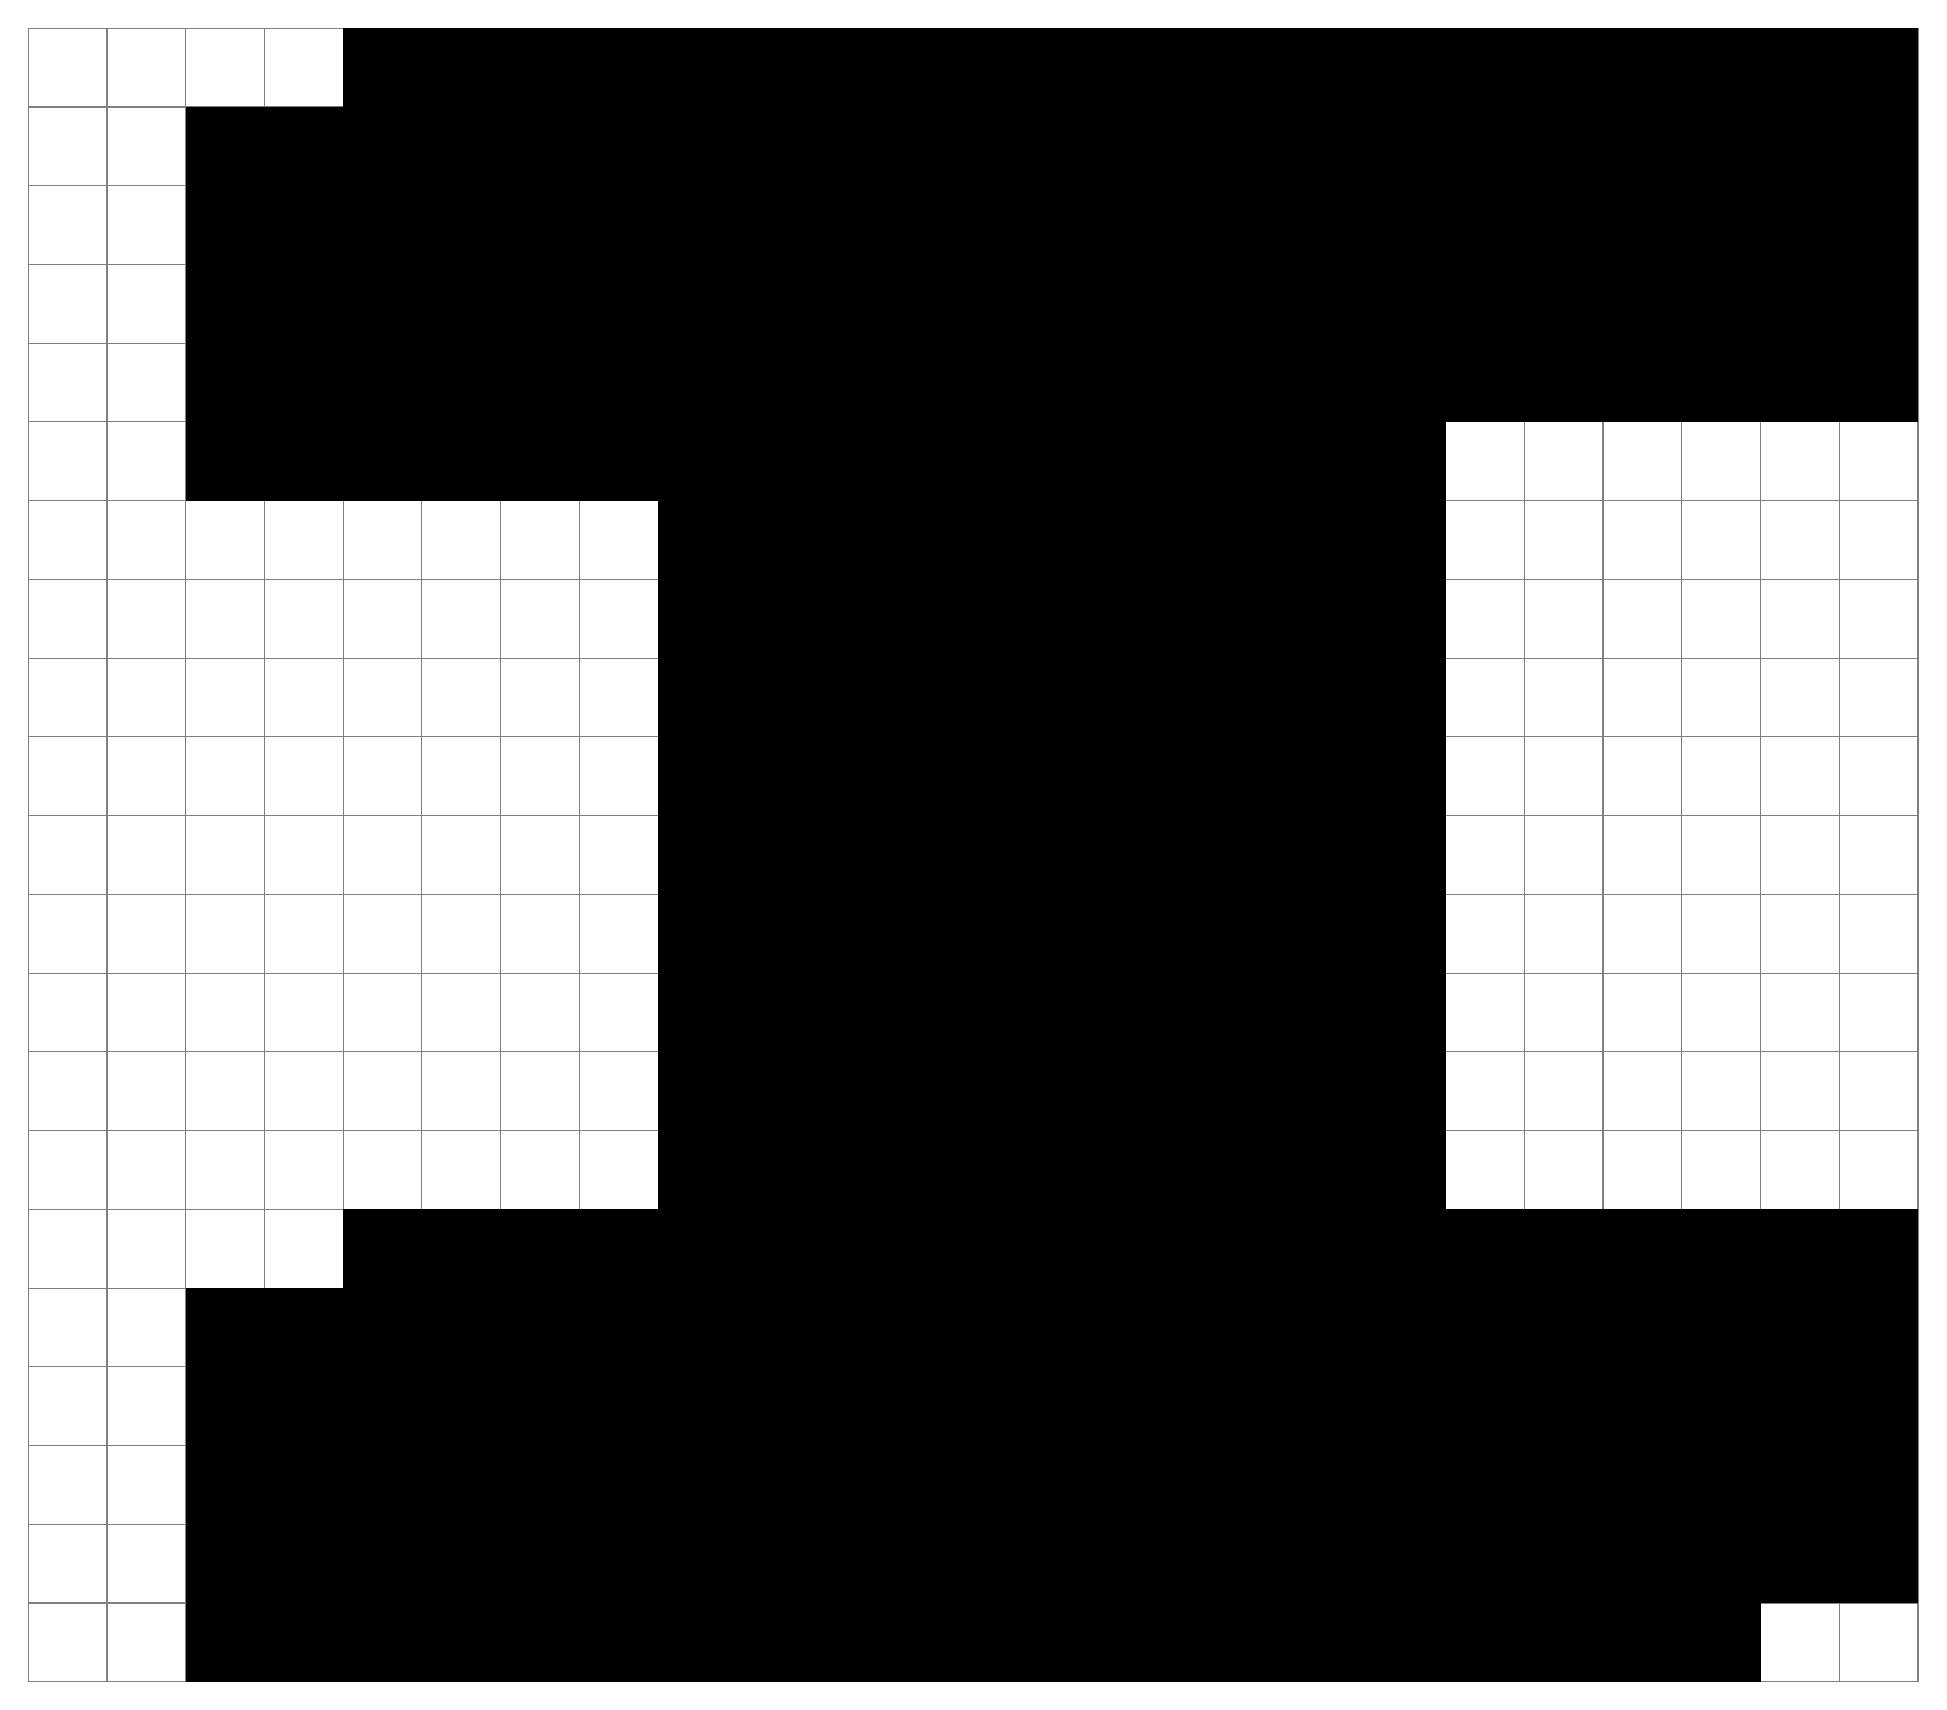
\begin{tikzpicture}

	\draw[step=1.0,gray,thin] (0,0) grid (24,21);
	\fill[\MULTICOLORTWO] (4,20) rectangle ++ (1,1);
	\fill[\MULTICOLORTWO] (5,20) rectangle ++ (1,1);
	\fill[\MULTICOLORTWO] (6,20) rectangle ++ (1,1);
	\fill[\MULTICOLORTWO] (7,20) rectangle ++ (1,1);
	\fill[\MULTICOLORTWO] (8,20) rectangle ++ (1,1);
	\fill[\MULTICOLORTWO] (9,20) rectangle ++ (1,1);
	\fill[\MULTICOLORTWO] (10,20) rectangle ++ (1,1);
	\fill[\MULTICOLORTWO] (11,20) rectangle ++ (1,1);
	\fill[\MULTICOLORTWO] (12,20) rectangle ++ (1,1);
	\fill[\MULTICOLORTWO] (13,20) rectangle ++ (1,1);
	\fill[\MULTICOLORTWO] (14,20) rectangle ++ (1,1);
	\fill[\MULTICOLORTWO] (15,20) rectangle ++ (1,1);
	\fill[\MULTICOLORTWO] (16,20) rectangle ++ (1,1);
	\fill[\MULTICOLORTWO] (17,20) rectangle ++ (1,1);
	\fill[\MULTICOLORTWO] (18,20) rectangle ++ (1,1);
	\fill[\MULTICOLORTWO] (19,20) rectangle ++ (1,1);
	\fill[\MULTICOLORTWO] (20,20) rectangle ++ (1,1);
	\fill[\MULTICOLORTWO] (21,20) rectangle ++ (1,1);
	\fill[\MULTICOLORTWO] (22,20) rectangle ++ (1,1);
	\fill[\MULTICOLORTWO] (23,20) rectangle ++ (1,1);
	\fill[\MULTICOLORONE] (2,19) rectangle ++ (1,1);
	\fill[\MULTICOLORONE] (3,19) rectangle ++ (1,1);
	\fill[\MULTICOLORTWO] (4,19) rectangle ++ (1,1);
	\fill[\MULTICOLORTWO] (5,19) rectangle ++ (1,1);
	\fill[\SPRITECOLOR] (6,19) rectangle ++ (1,1);
	\fill[\SPRITECOLOR] (7,19) rectangle ++ (1,1);
	\fill[\SPRITECOLOR] (8,19) rectangle ++ (1,1);
	\fill[\SPRITECOLOR] (9,19) rectangle ++ (1,1);
	\fill[\SPRITECOLOR] (10,19) rectangle ++ (1,1);
	\fill[\SPRITECOLOR] (11,19) rectangle ++ (1,1);
	\fill[\SPRITECOLOR] (12,19) rectangle ++ (1,1);
	\fill[\SPRITECOLOR] (13,19) rectangle ++ (1,1);
	\fill[\SPRITECOLOR] (14,19) rectangle ++ (1,1);
	\fill[\SPRITECOLOR] (15,19) rectangle ++ (1,1);
	\fill[\SPRITECOLOR] (16,19) rectangle ++ (1,1);
	\fill[\SPRITECOLOR] (17,19) rectangle ++ (1,1);
	\fill[\SPRITECOLOR] (18,19) rectangle ++ (1,1);
	\fill[\SPRITECOLOR] (19,19) rectangle ++ (1,1);
	\fill[\SPRITECOLOR] (20,19) rectangle ++ (1,1);
	\fill[\SPRITECOLOR] (21,19) rectangle ++ (1,1);
	\fill[\MULTICOLORTWO] (22,19) rectangle ++ (1,1);
	\fill[\MULTICOLORTWO] (23,19) rectangle ++ (1,1);
	\fill[\MULTICOLORONE] (2,18) rectangle ++ (1,1);
	\fill[\MULTICOLORONE] (3,18) rectangle ++ (1,1);
	\fill[\MULTICOLORTWO] (4,18) rectangle ++ (1,1);
	\fill[\MULTICOLORTWO] (5,18) rectangle ++ (1,1);
	\fill[\SPRITECOLOR] (6,18) rectangle ++ (1,1);
	\fill[\SPRITECOLOR] (7,18) rectangle ++ (1,1);
	\fill[\SPRITECOLOR] (8,18) rectangle ++ (1,1);
	\fill[\SPRITECOLOR] (9,18) rectangle ++ (1,1);
	\fill[\SPRITECOLOR] (10,18) rectangle ++ (1,1);
	\fill[\SPRITECOLOR] (11,18) rectangle ++ (1,1);
	\fill[\SPRITECOLOR] (12,18) rectangle ++ (1,1);
	\fill[\SPRITECOLOR] (13,18) rectangle ++ (1,1);
	\fill[\SPRITECOLOR] (14,18) rectangle ++ (1,1);
	\fill[\SPRITECOLOR] (15,18) rectangle ++ (1,1);
	\fill[\SPRITECOLOR] (16,18) rectangle ++ (1,1);
	\fill[\SPRITECOLOR] (17,18) rectangle ++ (1,1);
	\fill[\SPRITECOLOR] (18,18) rectangle ++ (1,1);
	\fill[\SPRITECOLOR] (19,18) rectangle ++ (1,1);
	\fill[\SPRITECOLOR] (20,18) rectangle ++ (1,1);
	\fill[\SPRITECOLOR] (21,18) rectangle ++ (1,1);
	\fill[\MULTICOLORTWO] (22,18) rectangle ++ (1,1);
	\fill[\MULTICOLORTWO] (23,18) rectangle ++ (1,1);
	\fill[\MULTICOLORONE] (2,17) rectangle ++ (1,1);
	\fill[\MULTICOLORONE] (3,17) rectangle ++ (1,1);
	\fill[\MULTICOLORTWO] (4,17) rectangle ++ (1,1);
	\fill[\MULTICOLORTWO] (5,17) rectangle ++ (1,1);
	\fill[\SPRITECOLOR] (6,17) rectangle ++ (1,1);
	\fill[\SPRITECOLOR] (7,17) rectangle ++ (1,1);
	\fill[\SPRITECOLOR] (8,17) rectangle ++ (1,1);
	\fill[\SPRITECOLOR] (9,17) rectangle ++ (1,1);
	\fill[\SPRITECOLOR] (10,17) rectangle ++ (1,1);
	\fill[\SPRITECOLOR] (11,17) rectangle ++ (1,1);
	\fill[\SPRITECOLOR] (12,17) rectangle ++ (1,1);
	\fill[\SPRITECOLOR] (13,17) rectangle ++ (1,1);
	\fill[\SPRITECOLOR] (14,17) rectangle ++ (1,1);
	\fill[\SPRITECOLOR] (15,17) rectangle ++ (1,1);
	\fill[\SPRITECOLOR] (16,17) rectangle ++ (1,1);
	\fill[\SPRITECOLOR] (17,17) rectangle ++ (1,1);
	\fill[\SPRITECOLOR] (18,17) rectangle ++ (1,1);
	\fill[\SPRITECOLOR] (19,17) rectangle ++ (1,1);
	\fill[\SPRITECOLOR] (20,17) rectangle ++ (1,1);
	\fill[\SPRITECOLOR] (21,17) rectangle ++ (1,1);
	\fill[\MULTICOLORTWO] (22,17) rectangle ++ (1,1);
	\fill[\MULTICOLORTWO] (23,17) rectangle ++ (1,1);
	\fill[\MULTICOLORONE] (2,16) rectangle ++ (1,1);
	\fill[\MULTICOLORONE] (3,16) rectangle ++ (1,1);
	\fill[\MULTICOLORTWO] (4,16) rectangle ++ (1,1);
	\fill[\MULTICOLORTWO] (5,16) rectangle ++ (1,1);
	\fill[\MULTICOLORTWO] (6,16) rectangle ++ (1,1);
	\fill[\MULTICOLORTWO] (7,16) rectangle ++ (1,1);
	\fill[\MULTICOLORTWO] (8,16) rectangle ++ (1,1);
	\fill[\MULTICOLORTWO] (9,16) rectangle ++ (1,1);
	\fill[\MULTICOLORTWO] (10,16) rectangle ++ (1,1);
	\fill[\MULTICOLORTWO] (11,16) rectangle ++ (1,1);
	\fill[\SPRITECOLOR] (12,16) rectangle ++ (1,1);
	\fill[\SPRITECOLOR] (13,16) rectangle ++ (1,1);
	\fill[\SPRITECOLOR] (14,16) rectangle ++ (1,1);
	\fill[\SPRITECOLOR] (15,16) rectangle ++ (1,1);
	\fill[\MULTICOLORTWO] (16,16) rectangle ++ (1,1);
	\fill[\MULTICOLORTWO] (17,16) rectangle ++ (1,1);
	\fill[\MULTICOLORTWO] (18,16) rectangle ++ (1,1);
	\fill[\MULTICOLORTWO] (19,16) rectangle ++ (1,1);
	\fill[\MULTICOLORTWO] (20,16) rectangle ++ (1,1);
	\fill[\MULTICOLORTWO] (21,16) rectangle ++ (1,1);
	\fill[\MULTICOLORTWO] (22,16) rectangle ++ (1,1);
	\fill[\MULTICOLORTWO] (23,16) rectangle ++ (1,1);
	\fill[\MULTICOLORONE] (2,15) rectangle ++ (1,1);
	\fill[\MULTICOLORONE] (3,15) rectangle ++ (1,1);
	\fill[\MULTICOLORONE] (4,15) rectangle ++ (1,1);
	\fill[\MULTICOLORONE] (5,15) rectangle ++ (1,1);
	\fill[\MULTICOLORONE] (6,15) rectangle ++ (1,1);
	\fill[\MULTICOLORONE] (7,15) rectangle ++ (1,1);
	\fill[\MULTICOLORONE] (8,15) rectangle ++ (1,1);
	\fill[\MULTICOLORONE] (9,15) rectangle ++ (1,1);
	\fill[\MULTICOLORTWO] (10,15) rectangle ++ (1,1);
	\fill[\MULTICOLORTWO] (11,15) rectangle ++ (1,1);
	\fill[\SPRITECOLOR] (12,15) rectangle ++ (1,1);
	\fill[\SPRITECOLOR] (13,15) rectangle ++ (1,1);
	\fill[\SPRITECOLOR] (14,15) rectangle ++ (1,1);
	\fill[\SPRITECOLOR] (15,15) rectangle ++ (1,1);
	\fill[\MULTICOLORTWO] (16,15) rectangle ++ (1,1);
	\fill[\MULTICOLORTWO] (17,15) rectangle ++ (1,1);
	\fill[\MULTICOLORONE] (8,14) rectangle ++ (1,1);
	\fill[\MULTICOLORONE] (9,14) rectangle ++ (1,1);
	\fill[\MULTICOLORTWO] (10,14) rectangle ++ (1,1);
	\fill[\MULTICOLORTWO] (11,14) rectangle ++ (1,1);
	\fill[\SPRITECOLOR] (12,14) rectangle ++ (1,1);
	\fill[\SPRITECOLOR] (13,14) rectangle ++ (1,1);
	\fill[\SPRITECOLOR] (14,14) rectangle ++ (1,1);
	\fill[\SPRITECOLOR] (15,14) rectangle ++ (1,1);
	\fill[\MULTICOLORTWO] (16,14) rectangle ++ (1,1);
	\fill[\MULTICOLORTWO] (17,14) rectangle ++ (1,1);
	\fill[\MULTICOLORONE] (8,13) rectangle ++ (1,1);
	\fill[\MULTICOLORONE] (9,13) rectangle ++ (1,1);
	\fill[\MULTICOLORTWO] (10,13) rectangle ++ (1,1);
	\fill[\MULTICOLORTWO] (11,13) rectangle ++ (1,1);
	\fill[\SPRITECOLOR] (12,13) rectangle ++ (1,1);
	\fill[\SPRITECOLOR] (13,13) rectangle ++ (1,1);
	\fill[\SPRITECOLOR] (14,13) rectangle ++ (1,1);
	\fill[\SPRITECOLOR] (15,13) rectangle ++ (1,1);
	\fill[\MULTICOLORTWO] (16,13) rectangle ++ (1,1);
	\fill[\MULTICOLORTWO] (17,13) rectangle ++ (1,1);
	\fill[\MULTICOLORONE] (8,12) rectangle ++ (1,1);
	\fill[\MULTICOLORONE] (9,12) rectangle ++ (1,1);
	\fill[\MULTICOLORTWO] (10,12) rectangle ++ (1,1);
	\fill[\MULTICOLORTWO] (11,12) rectangle ++ (1,1);
	\fill[\SPRITECOLOR] (12,12) rectangle ++ (1,1);
	\fill[\SPRITECOLOR] (13,12) rectangle ++ (1,1);
	\fill[\SPRITECOLOR] (14,12) rectangle ++ (1,1);
	\fill[\SPRITECOLOR] (15,12) rectangle ++ (1,1);
	\fill[\MULTICOLORTWO] (16,12) rectangle ++ (1,1);
	\fill[\MULTICOLORTWO] (17,12) rectangle ++ (1,1);
	\fill[\MULTICOLORONE] (8,11) rectangle ++ (1,1);
	\fill[\MULTICOLORONE] (9,11) rectangle ++ (1,1);
	\fill[\MULTICOLORTWO] (10,11) rectangle ++ (1,1);
	\fill[\MULTICOLORTWO] (11,11) rectangle ++ (1,1);
	\fill[\SPRITECOLOR] (12,11) rectangle ++ (1,1);
	\fill[\SPRITECOLOR] (13,11) rectangle ++ (1,1);
	\fill[\SPRITECOLOR] (14,11) rectangle ++ (1,1);
	\fill[\SPRITECOLOR] (15,11) rectangle ++ (1,1);
	\fill[\MULTICOLORTWO] (16,11) rectangle ++ (1,1);
	\fill[\MULTICOLORTWO] (17,11) rectangle ++ (1,1);
	\fill[\MULTICOLORONE] (8,10) rectangle ++ (1,1);
	\fill[\MULTICOLORONE] (9,10) rectangle ++ (1,1);
	\fill[\MULTICOLORTWO] (10,10) rectangle ++ (1,1);
	\fill[\MULTICOLORTWO] (11,10) rectangle ++ (1,1);
	\fill[\SPRITECOLOR] (12,10) rectangle ++ (1,1);
	\fill[\SPRITECOLOR] (13,10) rectangle ++ (1,1);
	\fill[\SPRITECOLOR] (14,10) rectangle ++ (1,1);
	\fill[\SPRITECOLOR] (15,10) rectangle ++ (1,1);
	\fill[\MULTICOLORTWO] (16,10) rectangle ++ (1,1);
	\fill[\MULTICOLORTWO] (17,10) rectangle ++ (1,1);
	\fill[\MULTICOLORONE] (8,9) rectangle ++ (1,1);
	\fill[\MULTICOLORONE] (9,9) rectangle ++ (1,1);
	\fill[\MULTICOLORTWO] (10,9) rectangle ++ (1,1);
	\fill[\MULTICOLORTWO] (11,9) rectangle ++ (1,1);
	\fill[\SPRITECOLOR] (12,9) rectangle ++ (1,1);
	\fill[\SPRITECOLOR] (13,9) rectangle ++ (1,1);
	\fill[\SPRITECOLOR] (14,9) rectangle ++ (1,1);
	\fill[\SPRITECOLOR] (15,9) rectangle ++ (1,1);
	\fill[\MULTICOLORTWO] (16,9) rectangle ++ (1,1);
	\fill[\MULTICOLORTWO] (17,9) rectangle ++ (1,1);
	\fill[\MULTICOLORONE] (8,8) rectangle ++ (1,1);
	\fill[\MULTICOLORONE] (9,8) rectangle ++ (1,1);
	\fill[\MULTICOLORTWO] (10,8) rectangle ++ (1,1);
	\fill[\MULTICOLORTWO] (11,8) rectangle ++ (1,1);
	\fill[\SPRITECOLOR] (12,8) rectangle ++ (1,1);
	\fill[\SPRITECOLOR] (13,8) rectangle ++ (1,1);
	\fill[\SPRITECOLOR] (14,8) rectangle ++ (1,1);
	\fill[\SPRITECOLOR] (15,8) rectangle ++ (1,1);
	\fill[\MULTICOLORTWO] (16,8) rectangle ++ (1,1);
	\fill[\MULTICOLORTWO] (17,8) rectangle ++ (1,1);
	\fill[\MULTICOLORONE] (8,7) rectangle ++ (1,1);
	\fill[\MULTICOLORONE] (9,7) rectangle ++ (1,1);
	\fill[\MULTICOLORTWO] (10,7) rectangle ++ (1,1);
	\fill[\MULTICOLORTWO] (11,7) rectangle ++ (1,1);
	\fill[\SPRITECOLOR] (12,7) rectangle ++ (1,1);
	\fill[\SPRITECOLOR] (13,7) rectangle ++ (1,1);
	\fill[\SPRITECOLOR] (14,7) rectangle ++ (1,1);
	\fill[\SPRITECOLOR] (15,7) rectangle ++ (1,1);
	\fill[\MULTICOLORTWO] (16,7) rectangle ++ (1,1);
	\fill[\MULTICOLORTWO] (17,7) rectangle ++ (1,1);
	\fill[\MULTICOLORONE] (8,6) rectangle ++ (1,1);
	\fill[\MULTICOLORONE] (9,6) rectangle ++ (1,1);
	\fill[\MULTICOLORTWO] (10,6) rectangle ++ (1,1);
	\fill[\MULTICOLORTWO] (11,6) rectangle ++ (1,1);
	\fill[\SPRITECOLOR] (12,6) rectangle ++ (1,1);
	\fill[\SPRITECOLOR] (13,6) rectangle ++ (1,1);
	\fill[\SPRITECOLOR] (14,6) rectangle ++ (1,1);
	\fill[\SPRITECOLOR] (15,6) rectangle ++ (1,1);
	\fill[\MULTICOLORTWO] (16,6) rectangle ++ (1,1);
	\fill[\MULTICOLORTWO] (17,6) rectangle ++ (1,1);
	\fill[\MULTICOLORTWO] (4,5) rectangle ++ (1,1);
	\fill[\MULTICOLORTWO] (5,5) rectangle ++ (1,1);
	\fill[\MULTICOLORTWO] (6,5) rectangle ++ (1,1);
	\fill[\MULTICOLORTWO] (7,5) rectangle ++ (1,1);
	\fill[\MULTICOLORTWO] (8,5) rectangle ++ (1,1);
	\fill[\MULTICOLORTWO] (9,5) rectangle ++ (1,1);
	\fill[\MULTICOLORTWO] (10,5) rectangle ++ (1,1);
	\fill[\MULTICOLORTWO] (11,5) rectangle ++ (1,1);
	\fill[\SPRITECOLOR] (12,5) rectangle ++ (1,1);
	\fill[\SPRITECOLOR] (13,5) rectangle ++ (1,1);
	\fill[\SPRITECOLOR] (14,5) rectangle ++ (1,1);
	\fill[\SPRITECOLOR] (15,5) rectangle ++ (1,1);
	\fill[\MULTICOLORTWO] (16,5) rectangle ++ (1,1);
	\fill[\MULTICOLORTWO] (17,5) rectangle ++ (1,1);
	\fill[\MULTICOLORTWO] (18,5) rectangle ++ (1,1);
	\fill[\MULTICOLORTWO] (19,5) rectangle ++ (1,1);
	\fill[\MULTICOLORTWO] (20,5) rectangle ++ (1,1);
	\fill[\MULTICOLORTWO] (21,5) rectangle ++ (1,1);
	\fill[\MULTICOLORTWO] (22,5) rectangle ++ (1,1);
	\fill[\MULTICOLORTWO] (23,5) rectangle ++ (1,1);
	\fill[\MULTICOLORONE] (2,4) rectangle ++ (1,1);
	\fill[\MULTICOLORONE] (3,4) rectangle ++ (1,1);
	\fill[\MULTICOLORTWO] (4,4) rectangle ++ (1,1);
	\fill[\MULTICOLORTWO] (5,4) rectangle ++ (1,1);
	\fill[\SPRITECOLOR] (6,4) rectangle ++ (1,1);
	\fill[\SPRITECOLOR] (7,4) rectangle ++ (1,1);
	\fill[\SPRITECOLOR] (8,4) rectangle ++ (1,1);
	\fill[\SPRITECOLOR] (9,4) rectangle ++ (1,1);
	\fill[\SPRITECOLOR] (10,4) rectangle ++ (1,1);
	\fill[\SPRITECOLOR] (11,4) rectangle ++ (1,1);
	\fill[\SPRITECOLOR] (12,4) rectangle ++ (1,1);
	\fill[\SPRITECOLOR] (13,4) rectangle ++ (1,1);
	\fill[\SPRITECOLOR] (14,4) rectangle ++ (1,1);
	\fill[\SPRITECOLOR] (15,4) rectangle ++ (1,1);
	\fill[\SPRITECOLOR] (16,4) rectangle ++ (1,1);
	\fill[\SPRITECOLOR] (17,4) rectangle ++ (1,1);
	\fill[\SPRITECOLOR] (18,4) rectangle ++ (1,1);
	\fill[\SPRITECOLOR] (19,4) rectangle ++ (1,1);
	\fill[\SPRITECOLOR] (20,4) rectangle ++ (1,1);
	\fill[\SPRITECOLOR] (21,4) rectangle ++ (1,1);
	\fill[\MULTICOLORTWO] (22,4) rectangle ++ (1,1);
	\fill[\MULTICOLORTWO] (23,4) rectangle ++ (1,1);
	\fill[\MULTICOLORONE] (2,3) rectangle ++ (1,1);
	\fill[\MULTICOLORONE] (3,3) rectangle ++ (1,1);
	\fill[\MULTICOLORTWO] (4,3) rectangle ++ (1,1);
	\fill[\MULTICOLORTWO] (5,3) rectangle ++ (1,1);
	\fill[\SPRITECOLOR] (6,3) rectangle ++ (1,1);
	\fill[\SPRITECOLOR] (7,3) rectangle ++ (1,1);
	\fill[\SPRITECOLOR] (8,3) rectangle ++ (1,1);
	\fill[\SPRITECOLOR] (9,3) rectangle ++ (1,1);
	\fill[\SPRITECOLOR] (10,3) rectangle ++ (1,1);
	\fill[\SPRITECOLOR] (11,3) rectangle ++ (1,1);
	\fill[\SPRITECOLOR] (12,3) rectangle ++ (1,1);
	\fill[\SPRITECOLOR] (13,3) rectangle ++ (1,1);
	\fill[\SPRITECOLOR] (14,3) rectangle ++ (1,1);
	\fill[\SPRITECOLOR] (15,3) rectangle ++ (1,1);
	\fill[\SPRITECOLOR] (16,3) rectangle ++ (1,1);
	\fill[\SPRITECOLOR] (17,3) rectangle ++ (1,1);
	\fill[\SPRITECOLOR] (18,3) rectangle ++ (1,1);
	\fill[\SPRITECOLOR] (19,3) rectangle ++ (1,1);
	\fill[\SPRITECOLOR] (20,3) rectangle ++ (1,1);
	\fill[\SPRITECOLOR] (21,3) rectangle ++ (1,1);
	\fill[\MULTICOLORTWO] (22,3) rectangle ++ (1,1);
	\fill[\MULTICOLORTWO] (23,3) rectangle ++ (1,1);
	\fill[\MULTICOLORONE] (2,2) rectangle ++ (1,1);
	\fill[\MULTICOLORONE] (3,2) rectangle ++ (1,1);
	\fill[\MULTICOLORTWO] (4,2) rectangle ++ (1,1);
	\fill[\MULTICOLORTWO] (5,2) rectangle ++ (1,1);
	\fill[\SPRITECOLOR] (6,2) rectangle ++ (1,1);
	\fill[\SPRITECOLOR] (7,2) rectangle ++ (1,1);
	\fill[\SPRITECOLOR] (8,2) rectangle ++ (1,1);
	\fill[\SPRITECOLOR] (9,2) rectangle ++ (1,1);
	\fill[\SPRITECOLOR] (10,2) rectangle ++ (1,1);
	\fill[\SPRITECOLOR] (11,2) rectangle ++ (1,1);
	\fill[\SPRITECOLOR] (12,2) rectangle ++ (1,1);
	\fill[\SPRITECOLOR] (13,2) rectangle ++ (1,1);
	\fill[\SPRITECOLOR] (14,2) rectangle ++ (1,1);
	\fill[\SPRITECOLOR] (15,2) rectangle ++ (1,1);
	\fill[\SPRITECOLOR] (16,2) rectangle ++ (1,1);
	\fill[\SPRITECOLOR] (17,2) rectangle ++ (1,1);
	\fill[\SPRITECOLOR] (18,2) rectangle ++ (1,1);
	\fill[\SPRITECOLOR] (19,2) rectangle ++ (1,1);
	\fill[\SPRITECOLOR] (20,2) rectangle ++ (1,1);
	\fill[\SPRITECOLOR] (21,2) rectangle ++ (1,1);
	\fill[\MULTICOLORTWO] (22,2) rectangle ++ (1,1);
	\fill[\MULTICOLORTWO] (23,2) rectangle ++ (1,1);
	\fill[\MULTICOLORONE] (2,1) rectangle ++ (1,1);
	\fill[\MULTICOLORONE] (3,1) rectangle ++ (1,1);
	\fill[\MULTICOLORTWO] (4,1) rectangle ++ (1,1);
	\fill[\MULTICOLORTWO] (5,1) rectangle ++ (1,1);
	\fill[\MULTICOLORTWO] (6,1) rectangle ++ (1,1);
	\fill[\MULTICOLORTWO] (7,1) rectangle ++ (1,1);
	\fill[\MULTICOLORTWO] (8,1) rectangle ++ (1,1);
	\fill[\MULTICOLORTWO] (9,1) rectangle ++ (1,1);
	\fill[\MULTICOLORTWO] (10,1) rectangle ++ (1,1);
	\fill[\MULTICOLORTWO] (11,1) rectangle ++ (1,1);
	\fill[\MULTICOLORTWO] (12,1) rectangle ++ (1,1);
	\fill[\MULTICOLORTWO] (13,1) rectangle ++ (1,1);
	\fill[\MULTICOLORTWO] (14,1) rectangle ++ (1,1);
	\fill[\MULTICOLORTWO] (15,1) rectangle ++ (1,1);
	\fill[\MULTICOLORTWO] (16,1) rectangle ++ (1,1);
	\fill[\MULTICOLORTWO] (17,1) rectangle ++ (1,1);
	\fill[\MULTICOLORTWO] (18,1) rectangle ++ (1,1);
	\fill[\MULTICOLORTWO] (19,1) rectangle ++ (1,1);
	\fill[\MULTICOLORTWO] (20,1) rectangle ++ (1,1);
	\fill[\MULTICOLORTWO] (21,1) rectangle ++ (1,1);
	\fill[\MULTICOLORTWO] (22,1) rectangle ++ (1,1);
	\fill[\MULTICOLORTWO] (23,1) rectangle ++ (1,1);
	\fill[\MULTICOLORONE] (2,0) rectangle ++ (1,1);
	\fill[\MULTICOLORONE] (3,0) rectangle ++ (1,1);
	\fill[\MULTICOLORONE] (4,0) rectangle ++ (1,1);
	\fill[\MULTICOLORONE] (5,0) rectangle ++ (1,1);
	\fill[\MULTICOLORONE] (6,0) rectangle ++ (1,1);
	\fill[\MULTICOLORONE] (7,0) rectangle ++ (1,1);
	\fill[\MULTICOLORONE] (8,0) rectangle ++ (1,1);
	\fill[\MULTICOLORONE] (9,0) rectangle ++ (1,1);
	\fill[\MULTICOLORONE] (10,0) rectangle ++ (1,1);
	\fill[\MULTICOLORONE] (11,0) rectangle ++ (1,1);
	\fill[\MULTICOLORONE] (12,0) rectangle ++ (1,1);
	\fill[\MULTICOLORONE] (13,0) rectangle ++ (1,1);
	\fill[\MULTICOLORONE] (14,0) rectangle ++ (1,1);
	\fill[\MULTICOLORONE] (15,0) rectangle ++ (1,1);
	\fill[\MULTICOLORONE] (16,0) rectangle ++ (1,1);
	\fill[\MULTICOLORONE] (17,0) rectangle ++ (1,1);
	\fill[\MULTICOLORONE] (18,0) rectangle ++ (1,1);
	\fill[\MULTICOLORONE] (19,0) rectangle ++ (1,1);
	\fill[\MULTICOLORONE] (20,0) rectangle ++ (1,1);
	\fill[\MULTICOLORONE] (21,0) rectangle ++ (1,1);

      \end{tikzpicture}
    \end{adjustbox}
  }\caption{BIG\_I}
\end{figure}

	\end{subfigure}
} &
\makecell[l]{
	\begin{subfigure}{0.3\textwidth}
    \def\MULTICOLORONE{gray}
    \def\MULTICOLORTWO{black}
    \def\SPRITECOLOR{gray}
		
\begin{figure}[H]
  {
    \setlength{\tabcolsep}{3.0pt}
    \setlength\cmidrulewidth{\heavyrulewidth} % Make cmidrule = 
    \begin{adjustbox}{width=3cm,center}
      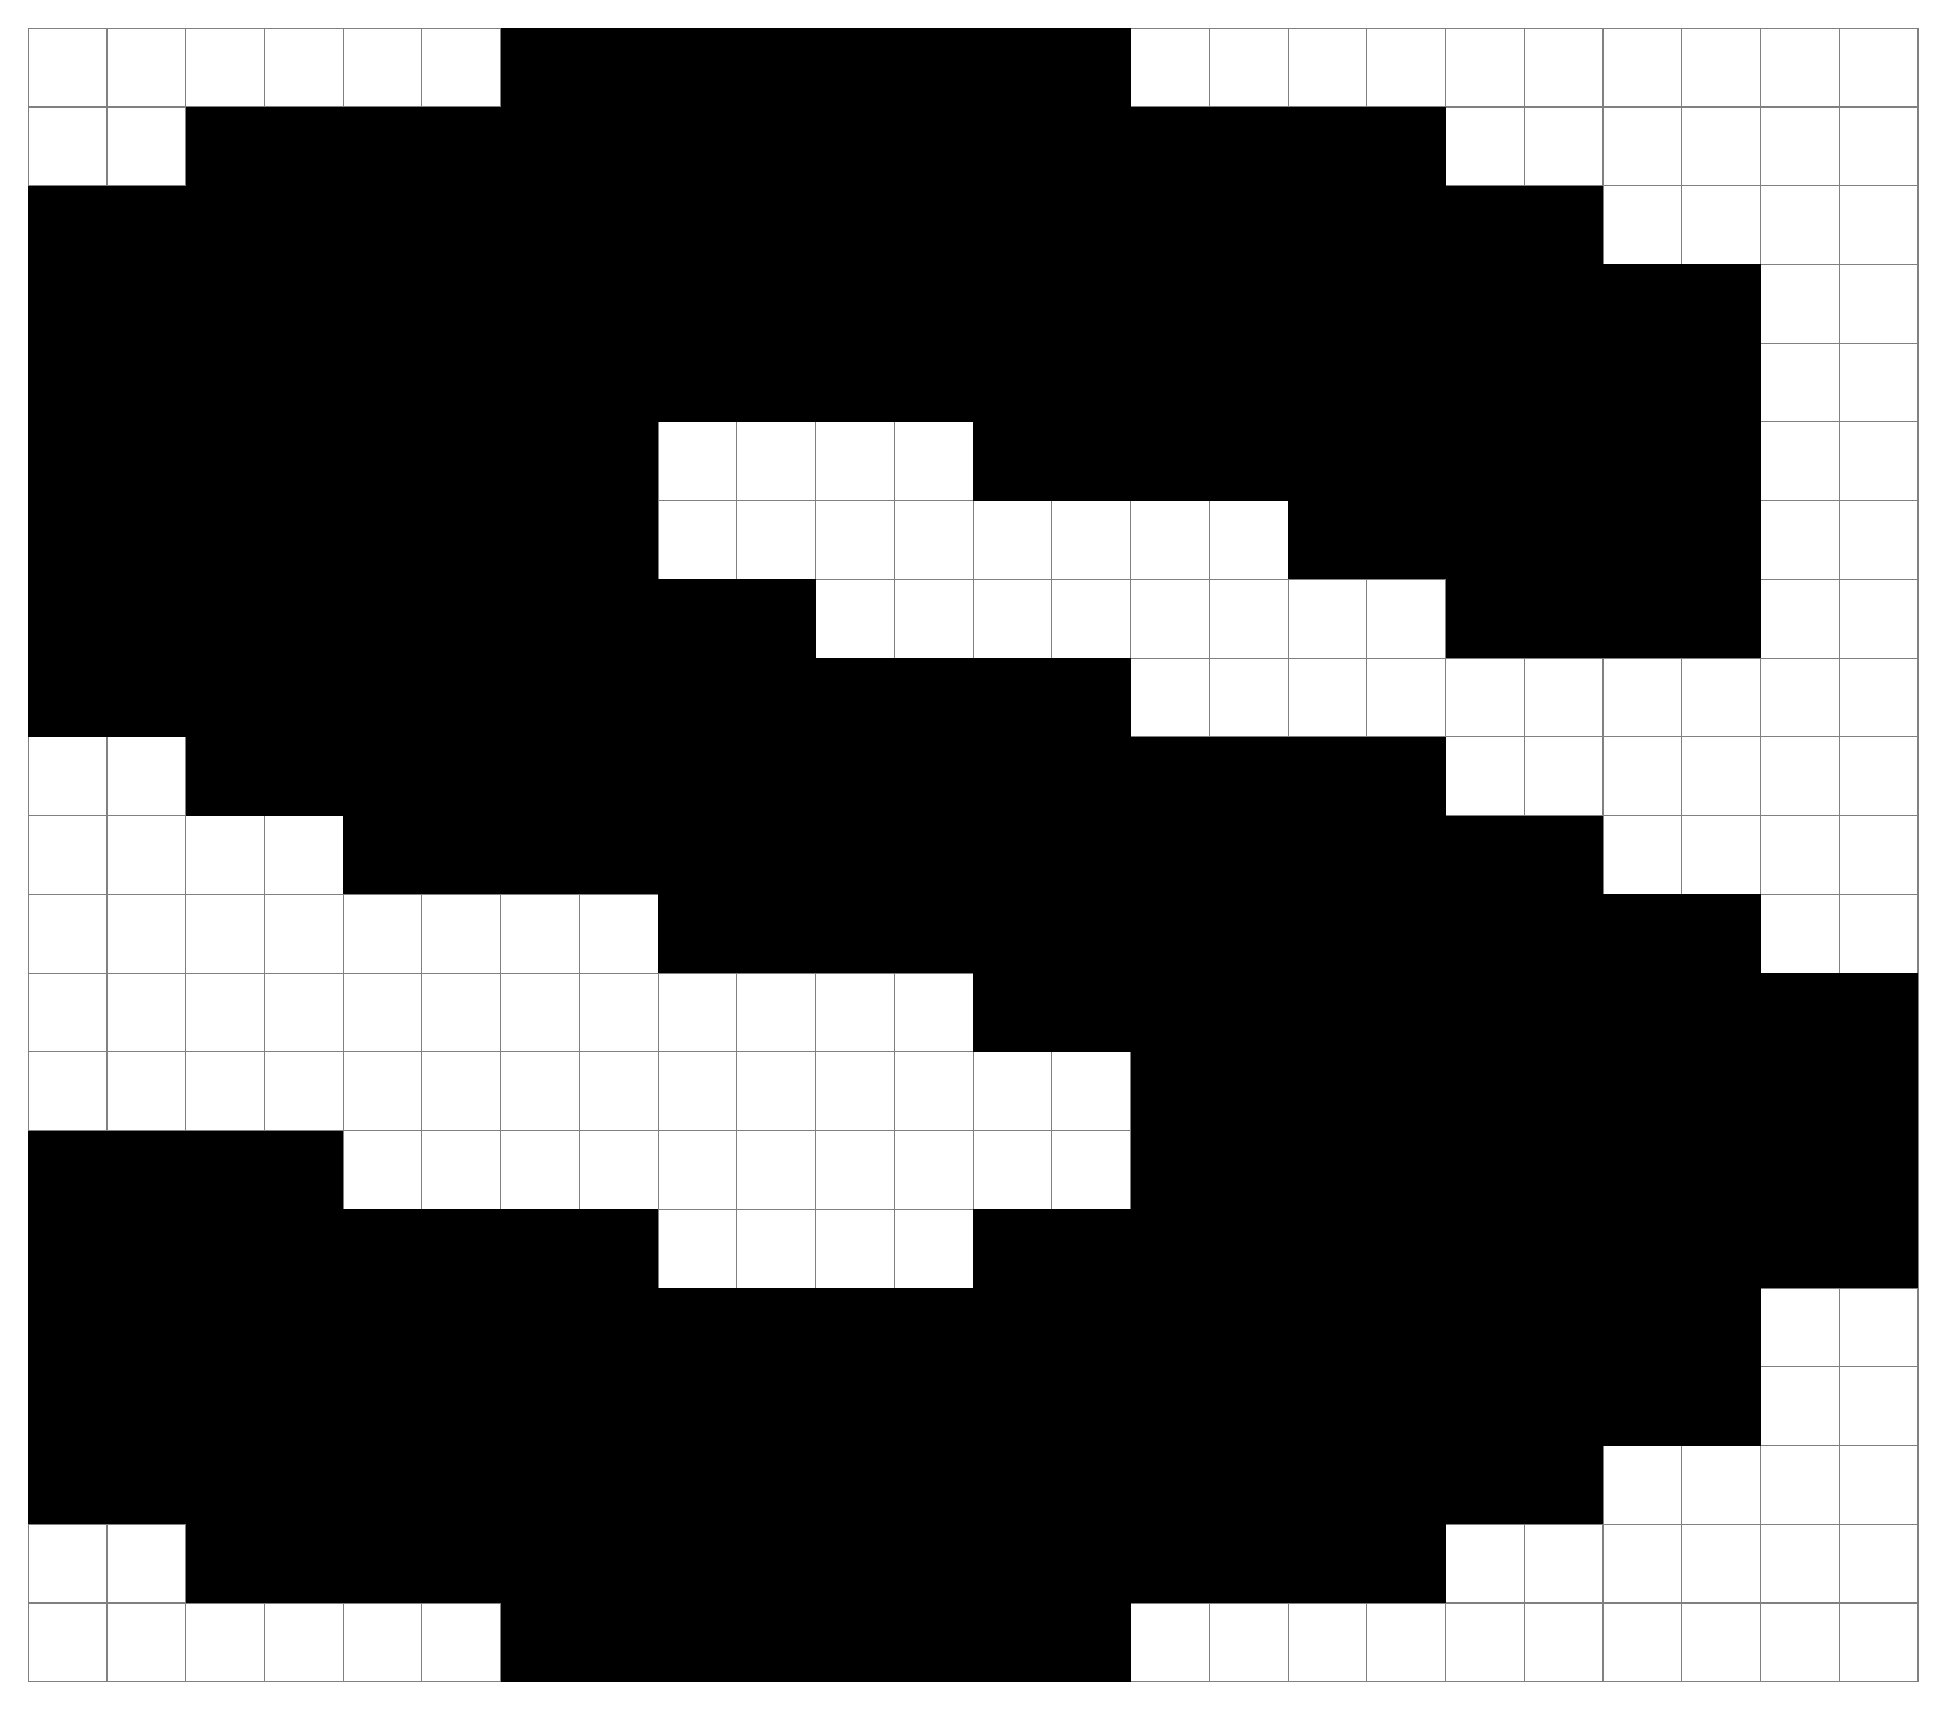
\begin{tikzpicture}

	\draw[step=1.0,gray,thin] (0,0) grid (24,21);
	\fill[\MULTICOLORONE] (6,20) rectangle ++ (1,1);
	\fill[\MULTICOLORONE] (7,20) rectangle ++ (1,1);
	\fill[\MULTICOLORTWO] (8,20) rectangle ++ (1,1);
	\fill[\MULTICOLORTWO] (9,20) rectangle ++ (1,1);
	\fill[\MULTICOLORTWO] (10,20) rectangle ++ (1,1);
	\fill[\MULTICOLORTWO] (11,20) rectangle ++ (1,1);
	\fill[\MULTICOLORTWO] (12,20) rectangle ++ (1,1);
	\fill[\MULTICOLORTWO] (13,20) rectangle ++ (1,1);
	\fill[\MULTICOLORONE] (2,19) rectangle ++ (1,1);
	\fill[\MULTICOLORONE] (3,19) rectangle ++ (1,1);
	\fill[\MULTICOLORTWO] (4,19) rectangle ++ (1,1);
	\fill[\MULTICOLORTWO] (5,19) rectangle ++ (1,1);
	\fill[\MULTICOLORTWO] (6,19) rectangle ++ (1,1);
	\fill[\MULTICOLORTWO] (7,19) rectangle ++ (1,1);
	\fill[\SPRITECOLOR] (8,19) rectangle ++ (1,1);
	\fill[\SPRITECOLOR] (9,19) rectangle ++ (1,1);
	\fill[\SPRITECOLOR] (10,19) rectangle ++ (1,1);
	\fill[\SPRITECOLOR] (11,19) rectangle ++ (1,1);
	\fill[\SPRITECOLOR] (12,19) rectangle ++ (1,1);
	\fill[\SPRITECOLOR] (13,19) rectangle ++ (1,1);
	\fill[\MULTICOLORTWO] (14,19) rectangle ++ (1,1);
	\fill[\MULTICOLORTWO] (15,19) rectangle ++ (1,1);
	\fill[\MULTICOLORTWO] (16,19) rectangle ++ (1,1);
	\fill[\MULTICOLORTWO] (17,19) rectangle ++ (1,1);
	\fill[\MULTICOLORONE] (0,18) rectangle ++ (1,1);
	\fill[\MULTICOLORONE] (1,18) rectangle ++ (1,1);
	\fill[\MULTICOLORTWO] (2,18) rectangle ++ (1,1);
	\fill[\MULTICOLORTWO] (3,18) rectangle ++ (1,1);
	\fill[\SPRITECOLOR] (4,18) rectangle ++ (1,1);
	\fill[\SPRITECOLOR] (5,18) rectangle ++ (1,1);
	\fill[\SPRITECOLOR] (6,18) rectangle ++ (1,1);
	\fill[\SPRITECOLOR] (7,18) rectangle ++ (1,1);
	\fill[\SPRITECOLOR] (8,18) rectangle ++ (1,1);
	\fill[\SPRITECOLOR] (9,18) rectangle ++ (1,1);
	\fill[\SPRITECOLOR] (10,18) rectangle ++ (1,1);
	\fill[\SPRITECOLOR] (11,18) rectangle ++ (1,1);
	\fill[\SPRITECOLOR] (12,18) rectangle ++ (1,1);
	\fill[\SPRITECOLOR] (13,18) rectangle ++ (1,1);
	\fill[\SPRITECOLOR] (14,18) rectangle ++ (1,1);
	\fill[\SPRITECOLOR] (15,18) rectangle ++ (1,1);
	\fill[\SPRITECOLOR] (16,18) rectangle ++ (1,1);
	\fill[\SPRITECOLOR] (17,18) rectangle ++ (1,1);
	\fill[\MULTICOLORTWO] (18,18) rectangle ++ (1,1);
	\fill[\MULTICOLORTWO] (19,18) rectangle ++ (1,1);
	\fill[\MULTICOLORTWO] (0,17) rectangle ++ (1,1);
	\fill[\MULTICOLORTWO] (1,17) rectangle ++ (1,1);
	\fill[\SPRITECOLOR] (2,17) rectangle ++ (1,1);
	\fill[\SPRITECOLOR] (3,17) rectangle ++ (1,1);
	\fill[\SPRITECOLOR] (4,17) rectangle ++ (1,1);
	\fill[\SPRITECOLOR] (5,17) rectangle ++ (1,1);
	\fill[\SPRITECOLOR] (6,17) rectangle ++ (1,1);
	\fill[\SPRITECOLOR] (7,17) rectangle ++ (1,1);
	\fill[\SPRITECOLOR] (8,17) rectangle ++ (1,1);
	\fill[\SPRITECOLOR] (9,17) rectangle ++ (1,1);
	\fill[\SPRITECOLOR] (10,17) rectangle ++ (1,1);
	\fill[\SPRITECOLOR] (11,17) rectangle ++ (1,1);
	\fill[\SPRITECOLOR] (12,17) rectangle ++ (1,1);
	\fill[\SPRITECOLOR] (13,17) rectangle ++ (1,1);
	\fill[\SPRITECOLOR] (14,17) rectangle ++ (1,1);
	\fill[\SPRITECOLOR] (15,17) rectangle ++ (1,1);
	\fill[\SPRITECOLOR] (16,17) rectangle ++ (1,1);
	\fill[\SPRITECOLOR] (17,17) rectangle ++ (1,1);
	\fill[\SPRITECOLOR] (18,17) rectangle ++ (1,1);
	\fill[\SPRITECOLOR] (19,17) rectangle ++ (1,1);
	\fill[\MULTICOLORTWO] (20,17) rectangle ++ (1,1);
	\fill[\MULTICOLORTWO] (21,17) rectangle ++ (1,1);
	\fill[\MULTICOLORTWO] (0,16) rectangle ++ (1,1);
	\fill[\MULTICOLORTWO] (1,16) rectangle ++ (1,1);
	\fill[\SPRITECOLOR] (2,16) rectangle ++ (1,1);
	\fill[\SPRITECOLOR] (3,16) rectangle ++ (1,1);
	\fill[\SPRITECOLOR] (4,16) rectangle ++ (1,1);
	\fill[\SPRITECOLOR] (5,16) rectangle ++ (1,1);
	\fill[\SPRITECOLOR] (6,16) rectangle ++ (1,1);
	\fill[\SPRITECOLOR] (7,16) rectangle ++ (1,1);
	\fill[\MULTICOLORTWO] (8,16) rectangle ++ (1,1);
	\fill[\MULTICOLORTWO] (9,16) rectangle ++ (1,1);
	\fill[\MULTICOLORTWO] (10,16) rectangle ++ (1,1);
	\fill[\MULTICOLORTWO] (11,16) rectangle ++ (1,1);
	\fill[\MULTICOLORTWO] (12,16) rectangle ++ (1,1);
	\fill[\MULTICOLORTWO] (13,16) rectangle ++ (1,1);
	\fill[\SPRITECOLOR] (14,16) rectangle ++ (1,1);
	\fill[\SPRITECOLOR] (15,16) rectangle ++ (1,1);
	\fill[\SPRITECOLOR] (16,16) rectangle ++ (1,1);
	\fill[\SPRITECOLOR] (17,16) rectangle ++ (1,1);
	\fill[\SPRITECOLOR] (18,16) rectangle ++ (1,1);
	\fill[\SPRITECOLOR] (19,16) rectangle ++ (1,1);
	\fill[\MULTICOLORTWO] (20,16) rectangle ++ (1,1);
	\fill[\MULTICOLORTWO] (21,16) rectangle ++ (1,1);
	\fill[\MULTICOLORTWO] (0,15) rectangle ++ (1,1);
	\fill[\MULTICOLORTWO] (1,15) rectangle ++ (1,1);
	\fill[\SPRITECOLOR] (2,15) rectangle ++ (1,1);
	\fill[\SPRITECOLOR] (3,15) rectangle ++ (1,1);
	\fill[\SPRITECOLOR] (4,15) rectangle ++ (1,1);
	\fill[\SPRITECOLOR] (5,15) rectangle ++ (1,1);
	\fill[\MULTICOLORTWO] (6,15) rectangle ++ (1,1);
	\fill[\MULTICOLORTWO] (7,15) rectangle ++ (1,1);
	\fill[\MULTICOLORONE] (12,15) rectangle ++ (1,1);
	\fill[\MULTICOLORONE] (13,15) rectangle ++ (1,1);
	\fill[\MULTICOLORTWO] (14,15) rectangle ++ (1,1);
	\fill[\MULTICOLORTWO] (15,15) rectangle ++ (1,1);
	\fill[\MULTICOLORTWO] (16,15) rectangle ++ (1,1);
	\fill[\MULTICOLORTWO] (17,15) rectangle ++ (1,1);
	\fill[\SPRITECOLOR] (18,15) rectangle ++ (1,1);
	\fill[\SPRITECOLOR] (19,15) rectangle ++ (1,1);
	\fill[\MULTICOLORTWO] (20,15) rectangle ++ (1,1);
	\fill[\MULTICOLORTWO] (21,15) rectangle ++ (1,1);
	\fill[\MULTICOLORTWO] (0,14) rectangle ++ (1,1);
	\fill[\MULTICOLORTWO] (1,14) rectangle ++ (1,1);
	\fill[\SPRITECOLOR] (2,14) rectangle ++ (1,1);
	\fill[\SPRITECOLOR] (3,14) rectangle ++ (1,1);
	\fill[\SPRITECOLOR] (4,14) rectangle ++ (1,1);
	\fill[\SPRITECOLOR] (5,14) rectangle ++ (1,1);
	\fill[\MULTICOLORTWO] (6,14) rectangle ++ (1,1);
	\fill[\MULTICOLORTWO] (7,14) rectangle ++ (1,1);
	\fill[\MULTICOLORONE] (16,14) rectangle ++ (1,1);
	\fill[\MULTICOLORONE] (17,14) rectangle ++ (1,1);
	\fill[\MULTICOLORTWO] (18,14) rectangle ++ (1,1);
	\fill[\MULTICOLORTWO] (19,14) rectangle ++ (1,1);
	\fill[\MULTICOLORTWO] (20,14) rectangle ++ (1,1);
	\fill[\MULTICOLORTWO] (21,14) rectangle ++ (1,1);
	\fill[\MULTICOLORTWO] (0,13) rectangle ++ (1,1);
	\fill[\MULTICOLORTWO] (1,13) rectangle ++ (1,1);
	\fill[\SPRITECOLOR] (2,13) rectangle ++ (1,1);
	\fill[\SPRITECOLOR] (3,13) rectangle ++ (1,1);
	\fill[\SPRITECOLOR] (4,13) rectangle ++ (1,1);
	\fill[\SPRITECOLOR] (5,13) rectangle ++ (1,1);
	\fill[\SPRITECOLOR] (6,13) rectangle ++ (1,1);
	\fill[\SPRITECOLOR] (7,13) rectangle ++ (1,1);
	\fill[\MULTICOLORTWO] (8,13) rectangle ++ (1,1);
	\fill[\MULTICOLORTWO] (9,13) rectangle ++ (1,1);
	\fill[\MULTICOLORONE] (18,13) rectangle ++ (1,1);
	\fill[\MULTICOLORONE] (19,13) rectangle ++ (1,1);
	\fill[\MULTICOLORTWO] (20,13) rectangle ++ (1,1);
	\fill[\MULTICOLORTWO] (21,13) rectangle ++ (1,1);
	\fill[\MULTICOLORONE] (0,12) rectangle ++ (1,1);
	\fill[\MULTICOLORONE] (1,12) rectangle ++ (1,1);
	\fill[\MULTICOLORTWO] (2,12) rectangle ++ (1,1);
	\fill[\MULTICOLORTWO] (3,12) rectangle ++ (1,1);
	\fill[\SPRITECOLOR] (4,12) rectangle ++ (1,1);
	\fill[\SPRITECOLOR] (5,12) rectangle ++ (1,1);
	\fill[\SPRITECOLOR] (6,12) rectangle ++ (1,1);
	\fill[\SPRITECOLOR] (7,12) rectangle ++ (1,1);
	\fill[\SPRITECOLOR] (8,12) rectangle ++ (1,1);
	\fill[\SPRITECOLOR] (9,12) rectangle ++ (1,1);
	\fill[\MULTICOLORTWO] (10,12) rectangle ++ (1,1);
	\fill[\MULTICOLORTWO] (11,12) rectangle ++ (1,1);
	\fill[\MULTICOLORTWO] (12,12) rectangle ++ (1,1);
	\fill[\MULTICOLORTWO] (13,12) rectangle ++ (1,1);
	\fill[\MULTICOLORONE] (2,11) rectangle ++ (1,1);
	\fill[\MULTICOLORONE] (3,11) rectangle ++ (1,1);
	\fill[\MULTICOLORTWO] (4,11) rectangle ++ (1,1);
	\fill[\MULTICOLORTWO] (5,11) rectangle ++ (1,1);
	\fill[\SPRITECOLOR] (6,11) rectangle ++ (1,1);
	\fill[\SPRITECOLOR] (7,11) rectangle ++ (1,1);
	\fill[\SPRITECOLOR] (8,11) rectangle ++ (1,1);
	\fill[\SPRITECOLOR] (9,11) rectangle ++ (1,1);
	\fill[\SPRITECOLOR] (10,11) rectangle ++ (1,1);
	\fill[\SPRITECOLOR] (11,11) rectangle ++ (1,1);
	\fill[\SPRITECOLOR] (12,11) rectangle ++ (1,1);
	\fill[\SPRITECOLOR] (13,11) rectangle ++ (1,1);
	\fill[\MULTICOLORTWO] (14,11) rectangle ++ (1,1);
	\fill[\MULTICOLORTWO] (15,11) rectangle ++ (1,1);
	\fill[\MULTICOLORTWO] (16,11) rectangle ++ (1,1);
	\fill[\MULTICOLORTWO] (17,11) rectangle ++ (1,1);
	\fill[\MULTICOLORONE] (4,10) rectangle ++ (1,1);
	\fill[\MULTICOLORONE] (5,10) rectangle ++ (1,1);
	\fill[\MULTICOLORTWO] (6,10) rectangle ++ (1,1);
	\fill[\MULTICOLORTWO] (7,10) rectangle ++ (1,1);
	\fill[\MULTICOLORTWO] (8,10) rectangle ++ (1,1);
	\fill[\MULTICOLORTWO] (9,10) rectangle ++ (1,1);
	\fill[\SPRITECOLOR] (10,10) rectangle ++ (1,1);
	\fill[\SPRITECOLOR] (11,10) rectangle ++ (1,1);
	\fill[\SPRITECOLOR] (12,10) rectangle ++ (1,1);
	\fill[\SPRITECOLOR] (13,10) rectangle ++ (1,1);
	\fill[\SPRITECOLOR] (14,10) rectangle ++ (1,1);
	\fill[\SPRITECOLOR] (15,10) rectangle ++ (1,1);
	\fill[\SPRITECOLOR] (16,10) rectangle ++ (1,1);
	\fill[\SPRITECOLOR] (17,10) rectangle ++ (1,1);
	\fill[\MULTICOLORTWO] (18,10) rectangle ++ (1,1);
	\fill[\MULTICOLORTWO] (19,10) rectangle ++ (1,1);
	\fill[\MULTICOLORONE] (8,9) rectangle ++ (1,1);
	\fill[\MULTICOLORONE] (9,9) rectangle ++ (1,1);
	\fill[\MULTICOLORTWO] (10,9) rectangle ++ (1,1);
	\fill[\MULTICOLORTWO] (11,9) rectangle ++ (1,1);
	\fill[\MULTICOLORTWO] (12,9) rectangle ++ (1,1);
	\fill[\MULTICOLORTWO] (13,9) rectangle ++ (1,1);
	\fill[\SPRITECOLOR] (14,9) rectangle ++ (1,1);
	\fill[\SPRITECOLOR] (15,9) rectangle ++ (1,1);
	\fill[\SPRITECOLOR] (16,9) rectangle ++ (1,1);
	\fill[\SPRITECOLOR] (17,9) rectangle ++ (1,1);
	\fill[\SPRITECOLOR] (18,9) rectangle ++ (1,1);
	\fill[\SPRITECOLOR] (19,9) rectangle ++ (1,1);
	\fill[\MULTICOLORTWO] (20,9) rectangle ++ (1,1);
	\fill[\MULTICOLORTWO] (21,9) rectangle ++ (1,1);
	\fill[\MULTICOLORONE] (12,8) rectangle ++ (1,1);
	\fill[\MULTICOLORONE] (13,8) rectangle ++ (1,1);
	\fill[\MULTICOLORTWO] (14,8) rectangle ++ (1,1);
	\fill[\MULTICOLORTWO] (15,8) rectangle ++ (1,1);
	\fill[\SPRITECOLOR] (16,8) rectangle ++ (1,1);
	\fill[\SPRITECOLOR] (17,8) rectangle ++ (1,1);
	\fill[\SPRITECOLOR] (18,8) rectangle ++ (1,1);
	\fill[\SPRITECOLOR] (19,8) rectangle ++ (1,1);
	\fill[\SPRITECOLOR] (20,8) rectangle ++ (1,1);
	\fill[\SPRITECOLOR] (21,8) rectangle ++ (1,1);
	\fill[\MULTICOLORTWO] (22,8) rectangle ++ (1,1);
	\fill[\MULTICOLORTWO] (23,8) rectangle ++ (1,1);
	\fill[\MULTICOLORONE] (14,7) rectangle ++ (1,1);
	\fill[\MULTICOLORONE] (15,7) rectangle ++ (1,1);
	\fill[\MULTICOLORTWO] (16,7) rectangle ++ (1,1);
	\fill[\MULTICOLORTWO] (17,7) rectangle ++ (1,1);
	\fill[\SPRITECOLOR] (18,7) rectangle ++ (1,1);
	\fill[\SPRITECOLOR] (19,7) rectangle ++ (1,1);
	\fill[\SPRITECOLOR] (20,7) rectangle ++ (1,1);
	\fill[\SPRITECOLOR] (21,7) rectangle ++ (1,1);
	\fill[\MULTICOLORTWO] (22,7) rectangle ++ (1,1);
	\fill[\MULTICOLORTWO] (23,7) rectangle ++ (1,1);
	\fill[\MULTICOLORTWO] (0,6) rectangle ++ (1,1);
	\fill[\MULTICOLORTWO] (1,6) rectangle ++ (1,1);
	\fill[\MULTICOLORTWO] (2,6) rectangle ++ (1,1);
	\fill[\MULTICOLORTWO] (3,6) rectangle ++ (1,1);
	\fill[\MULTICOLORONE] (14,6) rectangle ++ (1,1);
	\fill[\MULTICOLORONE] (15,6) rectangle ++ (1,1);
	\fill[\MULTICOLORTWO] (16,6) rectangle ++ (1,1);
	\fill[\MULTICOLORTWO] (17,6) rectangle ++ (1,1);
	\fill[\SPRITECOLOR] (18,6) rectangle ++ (1,1);
	\fill[\SPRITECOLOR] (19,6) rectangle ++ (1,1);
	\fill[\SPRITECOLOR] (20,6) rectangle ++ (1,1);
	\fill[\SPRITECOLOR] (21,6) rectangle ++ (1,1);
	\fill[\MULTICOLORTWO] (22,6) rectangle ++ (1,1);
	\fill[\MULTICOLORTWO] (23,6) rectangle ++ (1,1);
	\fill[\MULTICOLORTWO] (0,5) rectangle ++ (1,1);
	\fill[\MULTICOLORTWO] (1,5) rectangle ++ (1,1);
	\fill[\SPRITECOLOR] (2,5) rectangle ++ (1,1);
	\fill[\SPRITECOLOR] (3,5) rectangle ++ (1,1);
	\fill[\MULTICOLORTWO] (4,5) rectangle ++ (1,1);
	\fill[\MULTICOLORTWO] (5,5) rectangle ++ (1,1);
	\fill[\MULTICOLORTWO] (6,5) rectangle ++ (1,1);
	\fill[\MULTICOLORTWO] (7,5) rectangle ++ (1,1);
	\fill[\MULTICOLORONE] (12,5) rectangle ++ (1,1);
	\fill[\MULTICOLORONE] (13,5) rectangle ++ (1,1);
	\fill[\MULTICOLORTWO] (14,5) rectangle ++ (1,1);
	\fill[\MULTICOLORTWO] (15,5) rectangle ++ (1,1);
	\fill[\SPRITECOLOR] (16,5) rectangle ++ (1,1);
	\fill[\SPRITECOLOR] (17,5) rectangle ++ (1,1);
	\fill[\SPRITECOLOR] (18,5) rectangle ++ (1,1);
	\fill[\SPRITECOLOR] (19,5) rectangle ++ (1,1);
	\fill[\SPRITECOLOR] (20,5) rectangle ++ (1,1);
	\fill[\SPRITECOLOR] (21,5) rectangle ++ (1,1);
	\fill[\MULTICOLORTWO] (22,5) rectangle ++ (1,1);
	\fill[\MULTICOLORTWO] (23,5) rectangle ++ (1,1);
	\fill[\MULTICOLORTWO] (0,4) rectangle ++ (1,1);
	\fill[\MULTICOLORTWO] (1,4) rectangle ++ (1,1);
	\fill[\SPRITECOLOR] (2,4) rectangle ++ (1,1);
	\fill[\SPRITECOLOR] (3,4) rectangle ++ (1,1);
	\fill[\SPRITECOLOR] (4,4) rectangle ++ (1,1);
	\fill[\SPRITECOLOR] (5,4) rectangle ++ (1,1);
	\fill[\SPRITECOLOR] (6,4) rectangle ++ (1,1);
	\fill[\SPRITECOLOR] (7,4) rectangle ++ (1,1);
	\fill[\MULTICOLORTWO] (8,4) rectangle ++ (1,1);
	\fill[\MULTICOLORTWO] (9,4) rectangle ++ (1,1);
	\fill[\MULTICOLORTWO] (10,4) rectangle ++ (1,1);
	\fill[\MULTICOLORTWO] (11,4) rectangle ++ (1,1);
	\fill[\MULTICOLORTWO] (12,4) rectangle ++ (1,1);
	\fill[\MULTICOLORTWO] (13,4) rectangle ++ (1,1);
	\fill[\SPRITECOLOR] (14,4) rectangle ++ (1,1);
	\fill[\SPRITECOLOR] (15,4) rectangle ++ (1,1);
	\fill[\SPRITECOLOR] (16,4) rectangle ++ (1,1);
	\fill[\SPRITECOLOR] (17,4) rectangle ++ (1,1);
	\fill[\SPRITECOLOR] (18,4) rectangle ++ (1,1);
	\fill[\SPRITECOLOR] (19,4) rectangle ++ (1,1);
	\fill[\MULTICOLORTWO] (20,4) rectangle ++ (1,1);
	\fill[\MULTICOLORTWO] (21,4) rectangle ++ (1,1);
	\fill[\MULTICOLORTWO] (0,3) rectangle ++ (1,1);
	\fill[\MULTICOLORTWO] (1,3) rectangle ++ (1,1);
	\fill[\SPRITECOLOR] (2,3) rectangle ++ (1,1);
	\fill[\SPRITECOLOR] (3,3) rectangle ++ (1,1);
	\fill[\SPRITECOLOR] (4,3) rectangle ++ (1,1);
	\fill[\SPRITECOLOR] (5,3) rectangle ++ (1,1);
	\fill[\SPRITECOLOR] (6,3) rectangle ++ (1,1);
	\fill[\SPRITECOLOR] (7,3) rectangle ++ (1,1);
	\fill[\SPRITECOLOR] (8,3) rectangle ++ (1,1);
	\fill[\SPRITECOLOR] (9,3) rectangle ++ (1,1);
	\fill[\SPRITECOLOR] (10,3) rectangle ++ (1,1);
	\fill[\SPRITECOLOR] (11,3) rectangle ++ (1,1);
	\fill[\SPRITECOLOR] (12,3) rectangle ++ (1,1);
	\fill[\SPRITECOLOR] (13,3) rectangle ++ (1,1);
	\fill[\SPRITECOLOR] (14,3) rectangle ++ (1,1);
	\fill[\SPRITECOLOR] (15,3) rectangle ++ (1,1);
	\fill[\SPRITECOLOR] (16,3) rectangle ++ (1,1);
	\fill[\SPRITECOLOR] (17,3) rectangle ++ (1,1);
	\fill[\SPRITECOLOR] (18,3) rectangle ++ (1,1);
	\fill[\SPRITECOLOR] (19,3) rectangle ++ (1,1);
	\fill[\MULTICOLORTWO] (20,3) rectangle ++ (1,1);
	\fill[\MULTICOLORTWO] (21,3) rectangle ++ (1,1);
	\fill[\MULTICOLORTWO] (0,2) rectangle ++ (1,1);
	\fill[\MULTICOLORTWO] (1,2) rectangle ++ (1,1);
	\fill[\MULTICOLORTWO] (2,2) rectangle ++ (1,1);
	\fill[\MULTICOLORTWO] (3,2) rectangle ++ (1,1);
	\fill[\SPRITECOLOR] (4,2) rectangle ++ (1,1);
	\fill[\SPRITECOLOR] (5,2) rectangle ++ (1,1);
	\fill[\SPRITECOLOR] (6,2) rectangle ++ (1,1);
	\fill[\SPRITECOLOR] (7,2) rectangle ++ (1,1);
	\fill[\SPRITECOLOR] (8,2) rectangle ++ (1,1);
	\fill[\SPRITECOLOR] (9,2) rectangle ++ (1,1);
	\fill[\SPRITECOLOR] (10,2) rectangle ++ (1,1);
	\fill[\SPRITECOLOR] (11,2) rectangle ++ (1,1);
	\fill[\SPRITECOLOR] (12,2) rectangle ++ (1,1);
	\fill[\SPRITECOLOR] (13,2) rectangle ++ (1,1);
	\fill[\SPRITECOLOR] (14,2) rectangle ++ (1,1);
	\fill[\SPRITECOLOR] (15,2) rectangle ++ (1,1);
	\fill[\SPRITECOLOR] (16,2) rectangle ++ (1,1);
	\fill[\SPRITECOLOR] (17,2) rectangle ++ (1,1);
	\fill[\MULTICOLORTWO] (18,2) rectangle ++ (1,1);
	\fill[\MULTICOLORTWO] (19,2) rectangle ++ (1,1);
	\fill[\MULTICOLORONE] (2,1) rectangle ++ (1,1);
	\fill[\MULTICOLORONE] (3,1) rectangle ++ (1,1);
	\fill[\MULTICOLORTWO] (4,1) rectangle ++ (1,1);
	\fill[\MULTICOLORTWO] (5,1) rectangle ++ (1,1);
	\fill[\MULTICOLORTWO] (6,1) rectangle ++ (1,1);
	\fill[\MULTICOLORTWO] (7,1) rectangle ++ (1,1);
	\fill[\SPRITECOLOR] (8,1) rectangle ++ (1,1);
	\fill[\SPRITECOLOR] (9,1) rectangle ++ (1,1);
	\fill[\SPRITECOLOR] (10,1) rectangle ++ (1,1);
	\fill[\SPRITECOLOR] (11,1) rectangle ++ (1,1);
	\fill[\SPRITECOLOR] (12,1) rectangle ++ (1,1);
	\fill[\SPRITECOLOR] (13,1) rectangle ++ (1,1);
	\fill[\MULTICOLORTWO] (14,1) rectangle ++ (1,1);
	\fill[\MULTICOLORTWO] (15,1) rectangle ++ (1,1);
	\fill[\MULTICOLORTWO] (16,1) rectangle ++ (1,1);
	\fill[\MULTICOLORTWO] (17,1) rectangle ++ (1,1);
	\fill[\MULTICOLORONE] (6,0) rectangle ++ (1,1);
	\fill[\MULTICOLORONE] (7,0) rectangle ++ (1,1);
	\fill[\MULTICOLORTWO] (8,0) rectangle ++ (1,1);
	\fill[\MULTICOLORTWO] (9,0) rectangle ++ (1,1);
	\fill[\MULTICOLORTWO] (10,0) rectangle ++ (1,1);
	\fill[\MULTICOLORTWO] (11,0) rectangle ++ (1,1);
	\fill[\MULTICOLORTWO] (12,0) rectangle ++ (1,1);
	\fill[\MULTICOLORTWO] (13,0) rectangle ++ (1,1);

      \end{tikzpicture}
    \end{adjustbox}
  }\caption{IG\_S}
\end{figure}

	\end{subfigure}
} &
\makecell[l]{
	\begin{subfigure}{0.3\textwidth}
    \def\MULTICOLORONE{gray}
    \def\MULTICOLORTWO{gray}
    \def\SPRITECOLOR{gray}
		
\begin{figure}[H]
  {
    \setlength{\tabcolsep}{3.0pt}
    \setlength\cmidrulewidth{\heavyrulewidth} % Make cmidrule = 
    \begin{adjustbox}{width=3cm,center}
      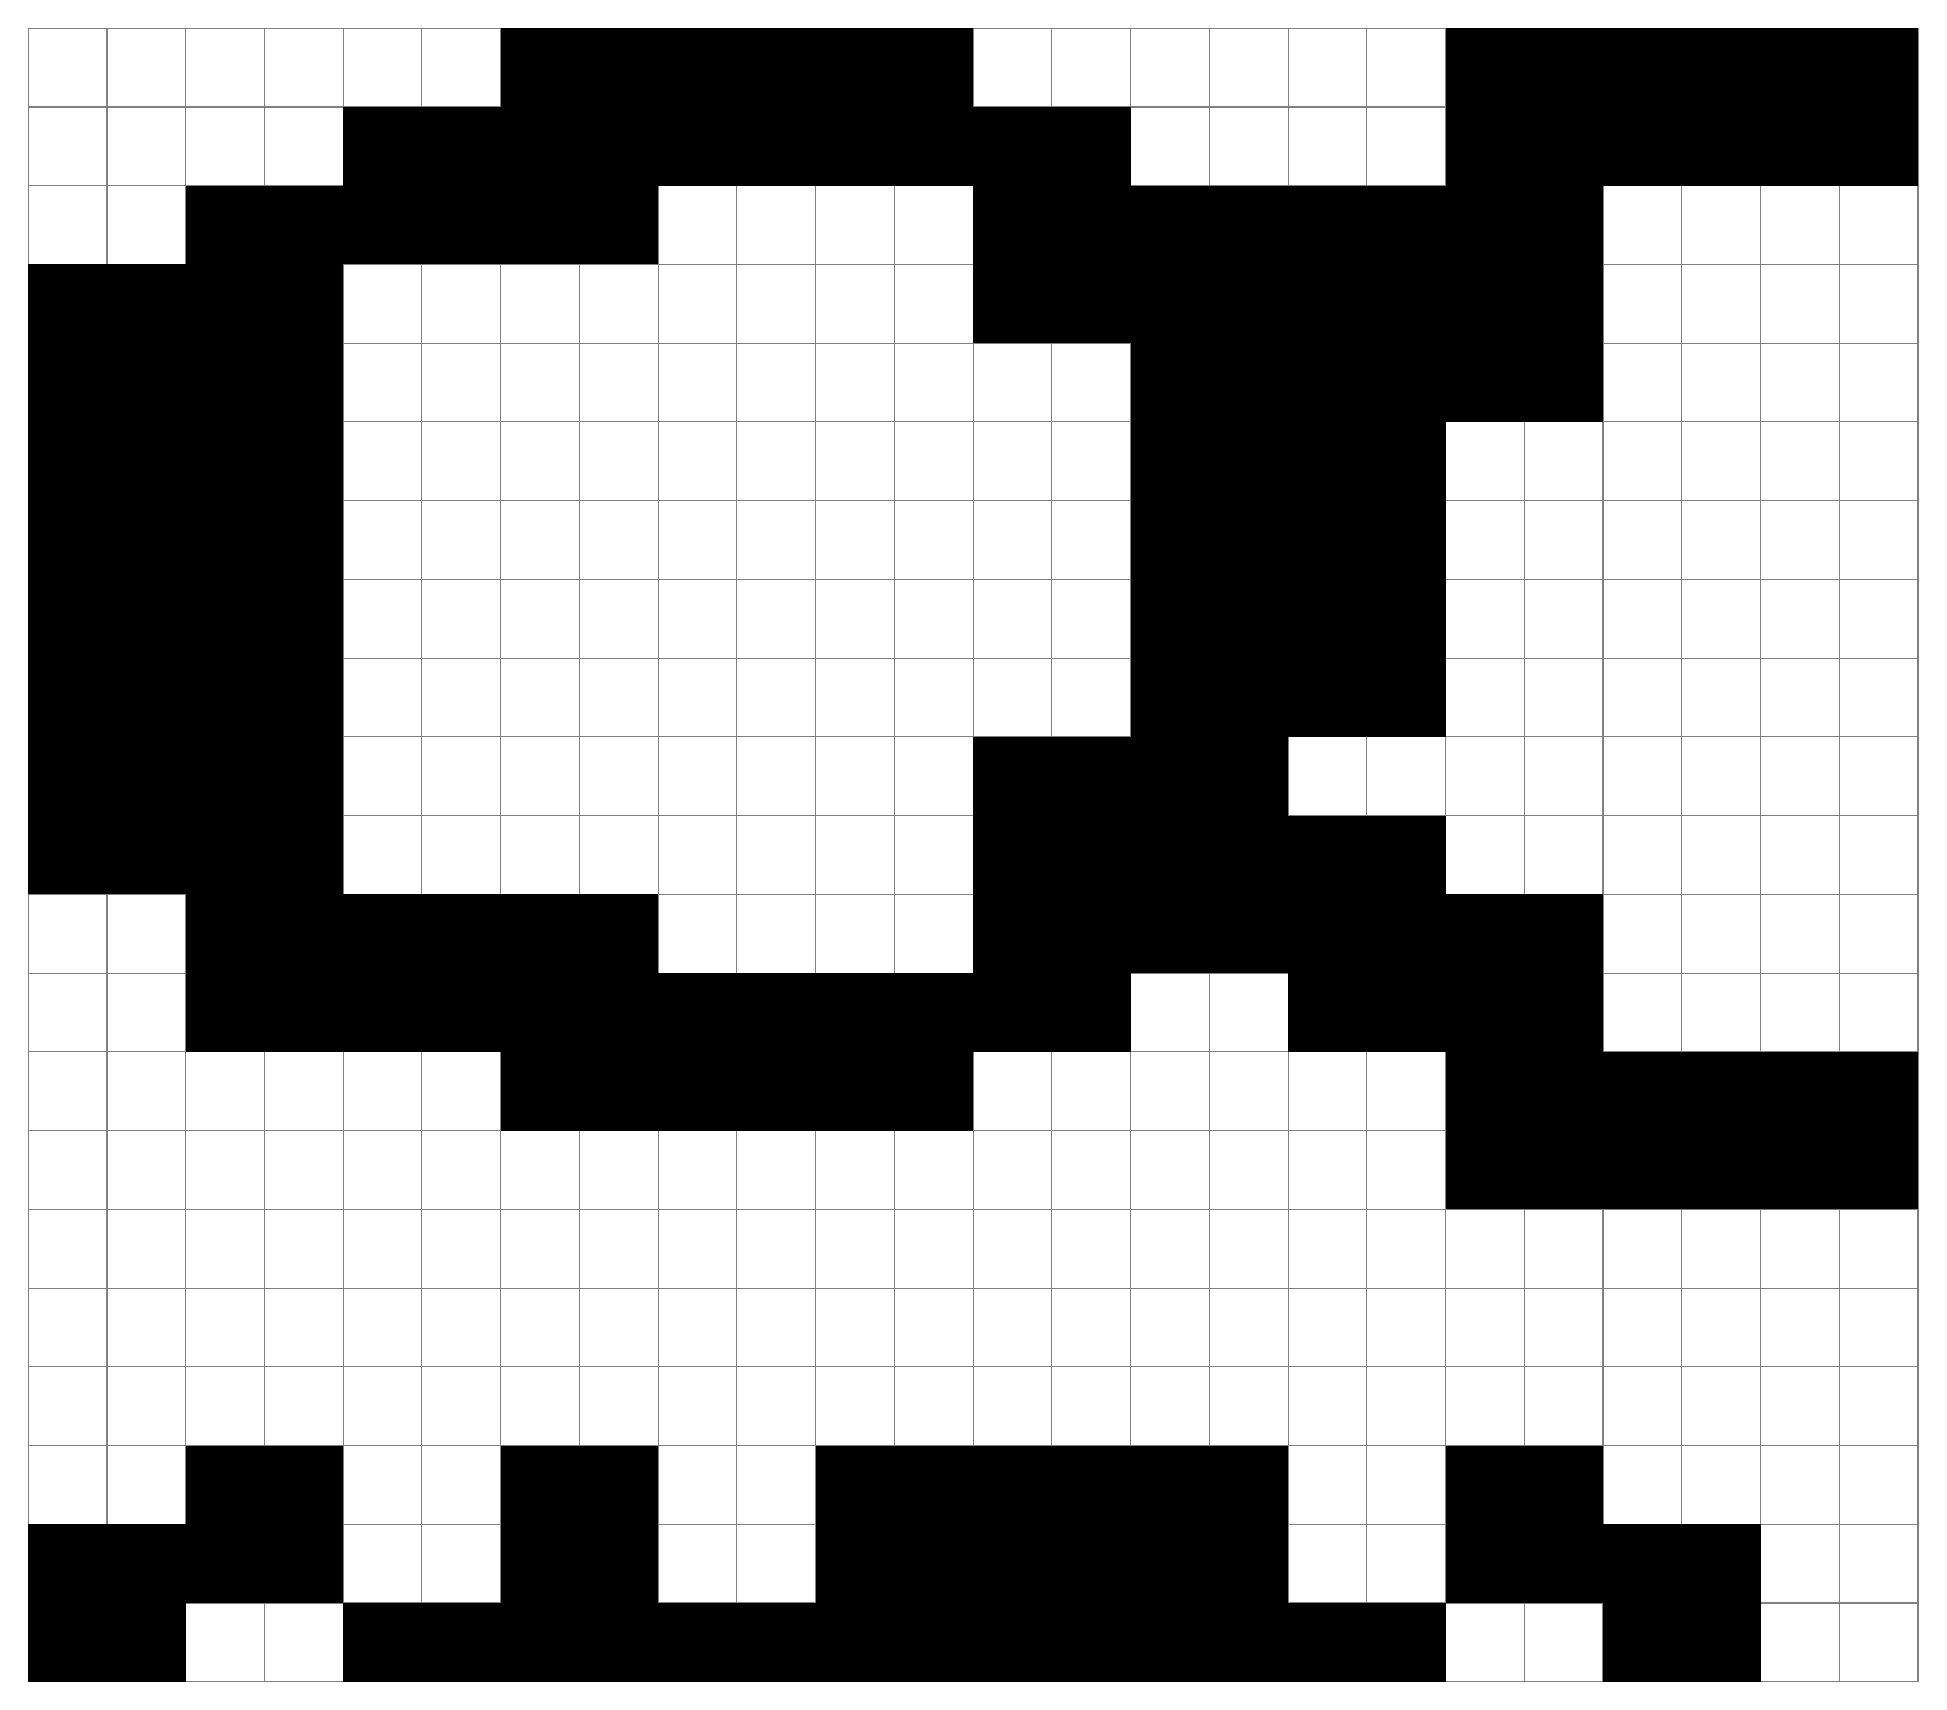
\begin{tikzpicture}

	\draw[step=1.0,gray,thin] (0,0) grid (24,21);
	\fill[\MULTICOLORONE] (6,20) rectangle ++ (1,1);
	\fill[\MULTICOLORONE] (7,20) rectangle ++ (1,1);
	\fill[\MULTICOLORTWO] (8,20) rectangle ++ (1,1);
	\fill[\MULTICOLORTWO] (9,20) rectangle ++ (1,1);
	\fill[\SPRITECOLOR] (10,20) rectangle ++ (1,1);
	\fill[\SPRITECOLOR] (11,20) rectangle ++ (1,1);
	\fill[\MULTICOLORONE] (18,20) rectangle ++ (1,1);
	\fill[\MULTICOLORONE] (19,20) rectangle ++ (1,1);
	\fill[\MULTICOLORTWO] (20,20) rectangle ++ (1,1);
	\fill[\MULTICOLORTWO] (21,20) rectangle ++ (1,1);
	\fill[\SPRITECOLOR] (22,20) rectangle ++ (1,1);
	\fill[\SPRITECOLOR] (23,20) rectangle ++ (1,1);
	\fill[\MULTICOLORTWO] (4,19) rectangle ++ (1,1);
	\fill[\MULTICOLORTWO] (5,19) rectangle ++ (1,1);
	\fill[\MULTICOLORTWO] (6,19) rectangle ++ (1,1);
	\fill[\MULTICOLORTWO] (7,19) rectangle ++ (1,1);
	\fill[\MULTICOLORTWO] (8,19) rectangle ++ (1,1);
	\fill[\MULTICOLORTWO] (9,19) rectangle ++ (1,1);
	\fill[\MULTICOLORTWO] (10,19) rectangle ++ (1,1);
	\fill[\MULTICOLORTWO] (11,19) rectangle ++ (1,1);
	\fill[\MULTICOLORTWO] (12,19) rectangle ++ (1,1);
	\fill[\MULTICOLORTWO] (13,19) rectangle ++ (1,1);
	\fill[\MULTICOLORTWO] (18,19) rectangle ++ (1,1);
	\fill[\MULTICOLORTWO] (19,19) rectangle ++ (1,1);
	\fill[\MULTICOLORTWO] (20,19) rectangle ++ (1,1);
	\fill[\MULTICOLORTWO] (21,19) rectangle ++ (1,1);
	\fill[\MULTICOLORTWO] (22,19) rectangle ++ (1,1);
	\fill[\MULTICOLORTWO] (23,19) rectangle ++ (1,1);
	\fill[\MULTICOLORTWO] (2,18) rectangle ++ (1,1);
	\fill[\MULTICOLORTWO] (3,18) rectangle ++ (1,1);
	\fill[\MULTICOLORTWO] (4,18) rectangle ++ (1,1);
	\fill[\MULTICOLORTWO] (5,18) rectangle ++ (1,1);
	\fill[\SPRITECOLOR] (6,18) rectangle ++ (1,1);
	\fill[\SPRITECOLOR] (7,18) rectangle ++ (1,1);
	\fill[\MULTICOLORTWO] (12,18) rectangle ++ (1,1);
	\fill[\MULTICOLORTWO] (13,18) rectangle ++ (1,1);
	\fill[\SPRITECOLOR] (14,18) rectangle ++ (1,1);
	\fill[\SPRITECOLOR] (15,18) rectangle ++ (1,1);
	\fill[\MULTICOLORONE] (16,18) rectangle ++ (1,1);
	\fill[\MULTICOLORONE] (17,18) rectangle ++ (1,1);
	\fill[\MULTICOLORTWO] (18,18) rectangle ++ (1,1);
	\fill[\MULTICOLORTWO] (19,18) rectangle ++ (1,1);
	\fill[\MULTICOLORONE] (0,17) rectangle ++ (1,1);
	\fill[\MULTICOLORONE] (1,17) rectangle ++ (1,1);
	\fill[\MULTICOLORTWO] (2,17) rectangle ++ (1,1);
	\fill[\MULTICOLORTWO] (3,17) rectangle ++ (1,1);
	\fill[\MULTICOLORONE] (12,17) rectangle ++ (1,1);
	\fill[\MULTICOLORONE] (13,17) rectangle ++ (1,1);
	\fill[\SPRITECOLOR] (14,17) rectangle ++ (1,1);
	\fill[\SPRITECOLOR] (15,17) rectangle ++ (1,1);
	\fill[\MULTICOLORTWO] (16,17) rectangle ++ (1,1);
	\fill[\MULTICOLORTWO] (17,17) rectangle ++ (1,1);
	\fill[\SPRITECOLOR] (18,17) rectangle ++ (1,1);
	\fill[\SPRITECOLOR] (19,17) rectangle ++ (1,1);
	\fill[\MULTICOLORONE] (0,16) rectangle ++ (1,1);
	\fill[\MULTICOLORONE] (1,16) rectangle ++ (1,1);
	\fill[\MULTICOLORTWO] (2,16) rectangle ++ (1,1);
	\fill[\MULTICOLORTWO] (3,16) rectangle ++ (1,1);
	\fill[\SPRITECOLOR] (14,16) rectangle ++ (1,1);
	\fill[\SPRITECOLOR] (15,16) rectangle ++ (1,1);
	\fill[\MULTICOLORTWO] (16,16) rectangle ++ (1,1);
	\fill[\MULTICOLORTWO] (17,16) rectangle ++ (1,1);
	\fill[\SPRITECOLOR] (18,16) rectangle ++ (1,1);
	\fill[\SPRITECOLOR] (19,16) rectangle ++ (1,1);
	\fill[\MULTICOLORTWO] (0,15) rectangle ++ (1,1);
	\fill[\MULTICOLORTWO] (1,15) rectangle ++ (1,1);
	\fill[\SPRITECOLOR] (2,15) rectangle ++ (1,1);
	\fill[\SPRITECOLOR] (3,15) rectangle ++ (1,1);
	\fill[\MULTICOLORONE] (14,15) rectangle ++ (1,1);
	\fill[\MULTICOLORONE] (15,15) rectangle ++ (1,1);
	\fill[\MULTICOLORTWO] (16,15) rectangle ++ (1,1);
	\fill[\MULTICOLORTWO] (17,15) rectangle ++ (1,1);
	\fill[\MULTICOLORTWO] (0,14) rectangle ++ (1,1);
	\fill[\MULTICOLORTWO] (1,14) rectangle ++ (1,1);
	\fill[\SPRITECOLOR] (2,14) rectangle ++ (1,1);
	\fill[\SPRITECOLOR] (3,14) rectangle ++ (1,1);
	\fill[\MULTICOLORONE] (14,14) rectangle ++ (1,1);
	\fill[\MULTICOLORONE] (15,14) rectangle ++ (1,1);
	\fill[\MULTICOLORTWO] (16,14) rectangle ++ (1,1);
	\fill[\MULTICOLORTWO] (17,14) rectangle ++ (1,1);
	\fill[\MULTICOLORTWO] (0,13) rectangle ++ (1,1);
	\fill[\MULTICOLORTWO] (1,13) rectangle ++ (1,1);
	\fill[\SPRITECOLOR] (2,13) rectangle ++ (1,1);
	\fill[\SPRITECOLOR] (3,13) rectangle ++ (1,1);
	\fill[\MULTICOLORTWO] (14,13) rectangle ++ (1,1);
	\fill[\MULTICOLORTWO] (15,13) rectangle ++ (1,1);
	\fill[\SPRITECOLOR] (16,13) rectangle ++ (1,1);
	\fill[\SPRITECOLOR] (17,13) rectangle ++ (1,1);
	\fill[\MULTICOLORTWO] (0,12) rectangle ++ (1,1);
	\fill[\MULTICOLORTWO] (1,12) rectangle ++ (1,1);
	\fill[\SPRITECOLOR] (2,12) rectangle ++ (1,1);
	\fill[\SPRITECOLOR] (3,12) rectangle ++ (1,1);
	\fill[\MULTICOLORTWO] (14,12) rectangle ++ (1,1);
	\fill[\MULTICOLORTWO] (15,12) rectangle ++ (1,1);
	\fill[\SPRITECOLOR] (16,12) rectangle ++ (1,1);
	\fill[\SPRITECOLOR] (17,12) rectangle ++ (1,1);
	\fill[\MULTICOLORONE] (0,11) rectangle ++ (1,1);
	\fill[\MULTICOLORONE] (1,11) rectangle ++ (1,1);
	\fill[\MULTICOLORTWO] (2,11) rectangle ++ (1,1);
	\fill[\MULTICOLORTWO] (3,11) rectangle ++ (1,1);
	\fill[\MULTICOLORONE] (12,11) rectangle ++ (1,1);
	\fill[\MULTICOLORONE] (13,11) rectangle ++ (1,1);
	\fill[\MULTICOLORTWO] (14,11) rectangle ++ (1,1);
	\fill[\MULTICOLORTWO] (15,11) rectangle ++ (1,1);
	\fill[\MULTICOLORONE] (0,10) rectangle ++ (1,1);
	\fill[\MULTICOLORONE] (1,10) rectangle ++ (1,1);
	\fill[\MULTICOLORTWO] (2,10) rectangle ++ (1,1);
	\fill[\MULTICOLORTWO] (3,10) rectangle ++ (1,1);
	\fill[\MULTICOLORONE] (12,10) rectangle ++ (1,1);
	\fill[\MULTICOLORONE] (13,10) rectangle ++ (1,1);
	\fill[\MULTICOLORTWO] (14,10) rectangle ++ (1,1);
	\fill[\MULTICOLORTWO] (15,10) rectangle ++ (1,1);
	\fill[\MULTICOLORONE] (16,10) rectangle ++ (1,1);
	\fill[\MULTICOLORONE] (17,10) rectangle ++ (1,1);
	\fill[\MULTICOLORTWO] (2,9) rectangle ++ (1,1);
	\fill[\MULTICOLORTWO] (3,9) rectangle ++ (1,1);
	\fill[\MULTICOLORTWO] (4,9) rectangle ++ (1,1);
	\fill[\MULTICOLORTWO] (5,9) rectangle ++ (1,1);
	\fill[\SPRITECOLOR] (6,9) rectangle ++ (1,1);
	\fill[\SPRITECOLOR] (7,9) rectangle ++ (1,1);
	\fill[\MULTICOLORTWO] (12,9) rectangle ++ (1,1);
	\fill[\MULTICOLORTWO] (13,9) rectangle ++ (1,1);
	\fill[\SPRITECOLOR] (14,9) rectangle ++ (1,1);
	\fill[\SPRITECOLOR] (15,9) rectangle ++ (1,1);
	\fill[\MULTICOLORONE] (16,9) rectangle ++ (1,1);
	\fill[\MULTICOLORONE] (17,9) rectangle ++ (1,1);
	\fill[\SPRITECOLOR] (18,9) rectangle ++ (1,1);
	\fill[\SPRITECOLOR] (19,9) rectangle ++ (1,1);
	\fill[\MULTICOLORONE] (2,8) rectangle ++ (1,1);
	\fill[\MULTICOLORONE] (3,8) rectangle ++ (1,1);
	\fill[\MULTICOLORTWO] (4,8) rectangle ++ (1,1);
	\fill[\MULTICOLORTWO] (5,8) rectangle ++ (1,1);
	\fill[\MULTICOLORTWO] (6,8) rectangle ++ (1,1);
	\fill[\MULTICOLORTWO] (7,8) rectangle ++ (1,1);
	\fill[\MULTICOLORTWO] (8,8) rectangle ++ (1,1);
	\fill[\MULTICOLORTWO] (9,8) rectangle ++ (1,1);
	\fill[\MULTICOLORTWO] (10,8) rectangle ++ (1,1);
	\fill[\MULTICOLORTWO] (11,8) rectangle ++ (1,1);
	\fill[\MULTICOLORTWO] (12,8) rectangle ++ (1,1);
	\fill[\MULTICOLORTWO] (13,8) rectangle ++ (1,1);
	\fill[\MULTICOLORONE] (16,8) rectangle ++ (1,1);
	\fill[\MULTICOLORONE] (17,8) rectangle ++ (1,1);
	\fill[\MULTICOLORTWO] (18,8) rectangle ++ (1,1);
	\fill[\MULTICOLORTWO] (19,8) rectangle ++ (1,1);
	\fill[\MULTICOLORONE] (6,7) rectangle ++ (1,1);
	\fill[\MULTICOLORONE] (7,7) rectangle ++ (1,1);
	\fill[\MULTICOLORTWO] (8,7) rectangle ++ (1,1);
	\fill[\MULTICOLORTWO] (9,7) rectangle ++ (1,1);
	\fill[\SPRITECOLOR] (10,7) rectangle ++ (1,1);
	\fill[\SPRITECOLOR] (11,7) rectangle ++ (1,1);
	\fill[\MULTICOLORTWO] (18,7) rectangle ++ (1,1);
	\fill[\MULTICOLORTWO] (19,7) rectangle ++ (1,1);
	\fill[\MULTICOLORTWO] (20,7) rectangle ++ (1,1);
	\fill[\MULTICOLORTWO] (21,7) rectangle ++ (1,1);
	\fill[\MULTICOLORTWO] (22,7) rectangle ++ (1,1);
	\fill[\MULTICOLORTWO] (23,7) rectangle ++ (1,1);
	\fill[\MULTICOLORONE] (18,6) rectangle ++ (1,1);
	\fill[\MULTICOLORONE] (19,6) rectangle ++ (1,1);
	\fill[\MULTICOLORTWO] (20,6) rectangle ++ (1,1);
	\fill[\MULTICOLORTWO] (21,6) rectangle ++ (1,1);
	\fill[\SPRITECOLOR] (22,6) rectangle ++ (1,1);
	\fill[\SPRITECOLOR] (23,6) rectangle ++ (1,1);
	\fill[\SPRITECOLOR] (2,2) rectangle ++ (1,1);
	\fill[\SPRITECOLOR] (3,2) rectangle ++ (1,1);
	\fill[\SPRITECOLOR] (6,2) rectangle ++ (1,1);
	\fill[\SPRITECOLOR] (7,2) rectangle ++ (1,1);
	\fill[\MULTICOLORTWO] (10,2) rectangle ++ (1,1);
	\fill[\MULTICOLORTWO] (11,2) rectangle ++ (1,1);
	\fill[\MULTICOLORONE] (12,2) rectangle ++ (1,1);
	\fill[\MULTICOLORONE] (13,2) rectangle ++ (1,1);
	\fill[\MULTICOLORONE] (14,2) rectangle ++ (1,1);
	\fill[\MULTICOLORONE] (15,2) rectangle ++ (1,1);
	\fill[\MULTICOLORONE] (18,2) rectangle ++ (1,1);
	\fill[\MULTICOLORONE] (19,2) rectangle ++ (1,1);
	\fill[\MULTICOLORONE] (0,1) rectangle ++ (1,1);
	\fill[\MULTICOLORONE] (1,1) rectangle ++ (1,1);
	\fill[\MULTICOLORONE] (2,1) rectangle ++ (1,1);
	\fill[\MULTICOLORONE] (3,1) rectangle ++ (1,1);
	\fill[\SPRITECOLOR] (6,1) rectangle ++ (1,1);
	\fill[\SPRITECOLOR] (7,1) rectangle ++ (1,1);
	\fill[\MULTICOLORTWO] (10,1) rectangle ++ (1,1);
	\fill[\MULTICOLORTWO] (11,1) rectangle ++ (1,1);
	\fill[\MULTICOLORONE] (12,1) rectangle ++ (1,1);
	\fill[\MULTICOLORONE] (13,1) rectangle ++ (1,1);
	\fill[\MULTICOLORTWO] (14,1) rectangle ++ (1,1);
	\fill[\MULTICOLORTWO] (15,1) rectangle ++ (1,1);
	\fill[\SPRITECOLOR] (18,1) rectangle ++ (1,1);
	\fill[\SPRITECOLOR] (19,1) rectangle ++ (1,1);
	\fill[\SPRITECOLOR] (20,1) rectangle ++ (1,1);
	\fill[\SPRITECOLOR] (21,1) rectangle ++ (1,1);
	\fill[\SPRITECOLOR] (0,0) rectangle ++ (1,1);
	\fill[\SPRITECOLOR] (1,0) rectangle ++ (1,1);
	\fill[\SPRITECOLOR] (4,0) rectangle ++ (1,1);
	\fill[\SPRITECOLOR] (5,0) rectangle ++ (1,1);
	\fill[\MULTICOLORTWO] (6,0) rectangle ++ (1,1);
	\fill[\MULTICOLORTWO] (7,0) rectangle ++ (1,1);
	\fill[\SPRITECOLOR] (8,0) rectangle ++ (1,1);
	\fill[\SPRITECOLOR] (9,0) rectangle ++ (1,1);
	\fill[\SPRITECOLOR] (10,0) rectangle ++ (1,1);
	\fill[\SPRITECOLOR] (11,0) rectangle ++ (1,1);
	\fill[\MULTICOLORONE] (12,0) rectangle ++ (1,1);
	\fill[\MULTICOLORONE] (13,0) rectangle ++ (1,1);
	\fill[\MULTICOLORONE] (14,0) rectangle ++ (1,1);
	\fill[\MULTICOLORONE] (15,0) rectangle ++ (1,1);
	\fill[\MULTICOLORONE] (16,0) rectangle ++ (1,1);
	\fill[\MULTICOLORONE] (17,0) rectangle ++ (1,1);
	\fill[\MULTICOLORONE] (20,0) rectangle ++ (1,1);
	\fill[\MULTICOLORONE] (21,0) rectangle ++ (1,1);

      \end{tikzpicture}
    \end{adjustbox}
  }\caption{ALPHA}
\end{figure}

	\end{subfigure}
} \\ 
        \midrule
\makecell[l]{
	\begin{subfigure}{0.3\textwidth}
    \def\MULTICOLORONE{gray}
    \def\MULTICOLORTWO{white}
    \def\SPRITECOLOR{red}
		
\begin{figure}[H]
  {
    \setlength{\tabcolsep}{3.0pt}
    \setlength\cmidrulewidth{\heavyrulewidth} % Make cmidrule = 
    \begin{adjustbox}{width=3cm,center}
      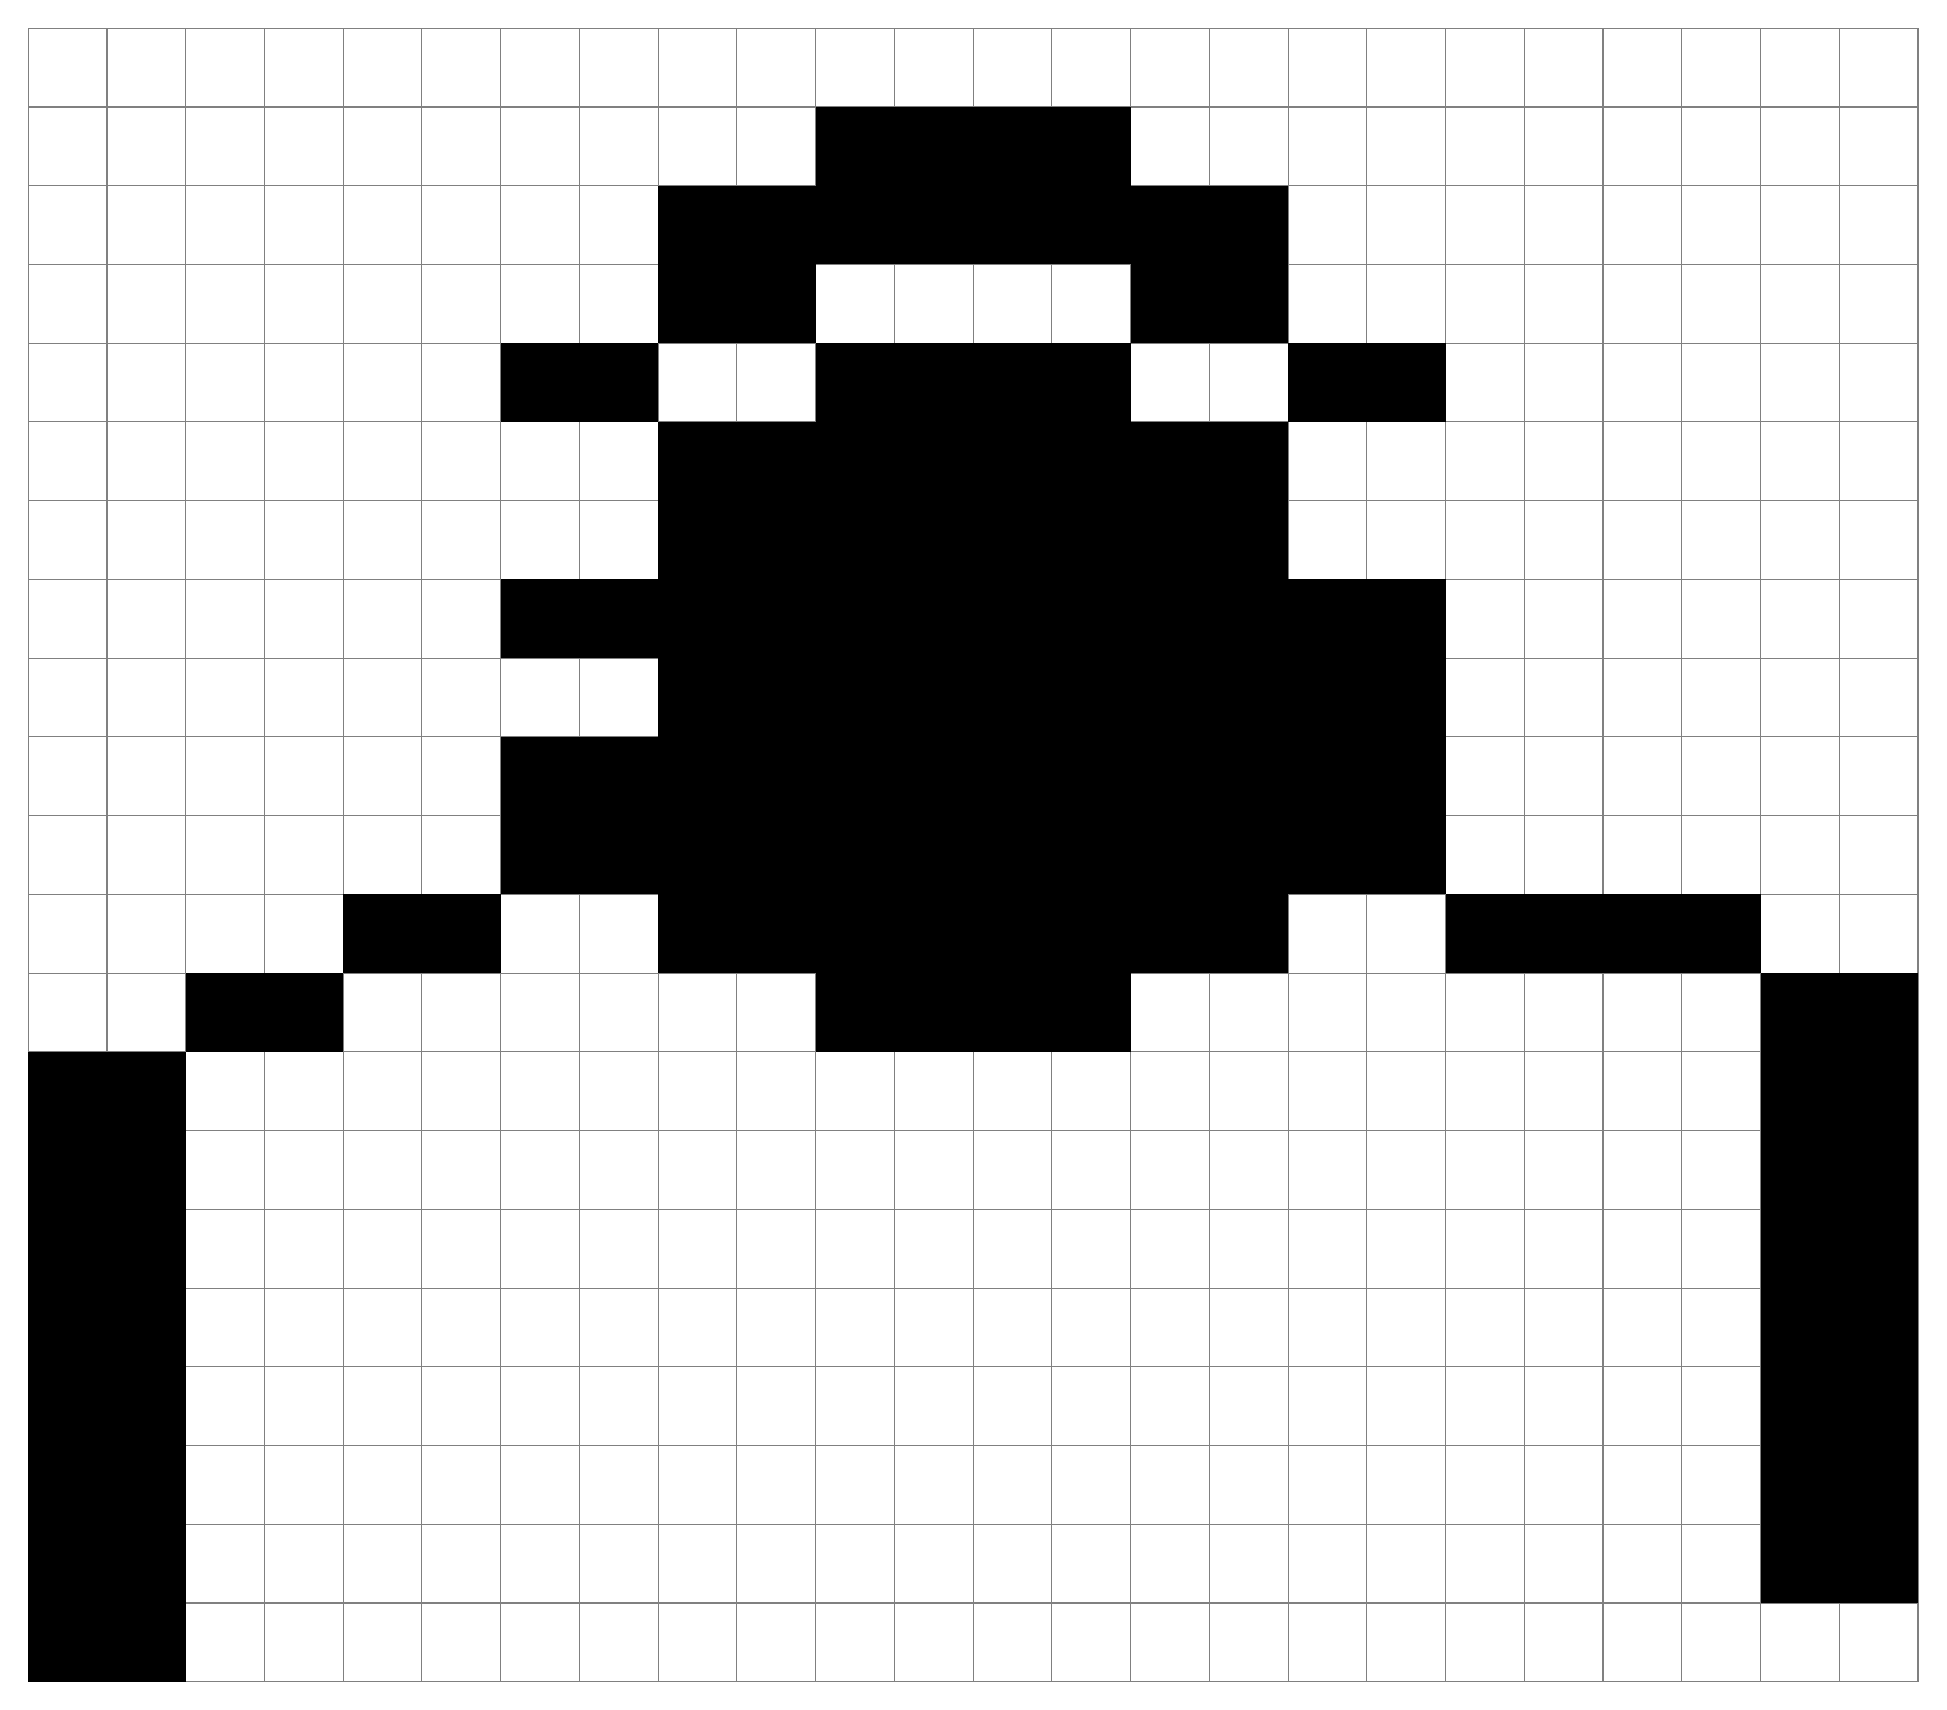
\begin{tikzpicture}

	\draw[step=1.0,gray,thin] (0,0) grid (24,21);
	\fill[\SPRITECOLOR] (10,19) rectangle ++ (1,1);
	\fill[\SPRITECOLOR] (11,19) rectangle ++ (1,1);
	\fill[\SPRITECOLOR] (12,19) rectangle ++ (1,1);
	\fill[\SPRITECOLOR] (13,19) rectangle ++ (1,1);
	\fill[\SPRITECOLOR] (8,18) rectangle ++ (1,1);
	\fill[\SPRITECOLOR] (9,18) rectangle ++ (1,1);
	\fill[\SPRITECOLOR] (10,18) rectangle ++ (1,1);
	\fill[\SPRITECOLOR] (11,18) rectangle ++ (1,1);
	\fill[\SPRITECOLOR] (12,18) rectangle ++ (1,1);
	\fill[\SPRITECOLOR] (13,18) rectangle ++ (1,1);
	\fill[\SPRITECOLOR] (14,18) rectangle ++ (1,1);
	\fill[\SPRITECOLOR] (15,18) rectangle ++ (1,1);
	\fill[\SPRITECOLOR] (8,17) rectangle ++ (1,1);
	\fill[\SPRITECOLOR] (9,17) rectangle ++ (1,1);
	\fill[\SPRITECOLOR] (14,17) rectangle ++ (1,1);
	\fill[\SPRITECOLOR] (15,17) rectangle ++ (1,1);
	\fill[\SPRITECOLOR] (6,16) rectangle ++ (1,1);
	\fill[\SPRITECOLOR] (7,16) rectangle ++ (1,1);
	\fill[\SPRITECOLOR] (10,16) rectangle ++ (1,1);
	\fill[\SPRITECOLOR] (11,16) rectangle ++ (1,1);
	\fill[\SPRITECOLOR] (12,16) rectangle ++ (1,1);
	\fill[\SPRITECOLOR] (13,16) rectangle ++ (1,1);
	\fill[\SPRITECOLOR] (16,16) rectangle ++ (1,1);
	\fill[\SPRITECOLOR] (17,16) rectangle ++ (1,1);
	\fill[\SPRITECOLOR] (8,15) rectangle ++ (1,1);
	\fill[\SPRITECOLOR] (9,15) rectangle ++ (1,1);
	\fill[\MULTICOLORTWO] (10,15) rectangle ++ (1,1);
	\fill[\MULTICOLORTWO] (11,15) rectangle ++ (1,1);
	\fill[\SPRITECOLOR] (12,15) rectangle ++ (1,1);
	\fill[\SPRITECOLOR] (13,15) rectangle ++ (1,1);
	\fill[\SPRITECOLOR] (14,15) rectangle ++ (1,1);
	\fill[\SPRITECOLOR] (15,15) rectangle ++ (1,1);
	\fill[\MULTICOLORTWO] (8,14) rectangle ++ (1,1);
	\fill[\MULTICOLORTWO] (9,14) rectangle ++ (1,1);
	\fill[\SPRITECOLOR] (10,14) rectangle ++ (1,1);
	\fill[\SPRITECOLOR] (11,14) rectangle ++ (1,1);
	\fill[\SPRITECOLOR] (12,14) rectangle ++ (1,1);
	\fill[\SPRITECOLOR] (13,14) rectangle ++ (1,1);
	\fill[\SPRITECOLOR] (14,14) rectangle ++ (1,1);
	\fill[\SPRITECOLOR] (15,14) rectangle ++ (1,1);
	\fill[\MULTICOLORTWO] (6,13) rectangle ++ (1,1);
	\fill[\MULTICOLORTWO] (7,13) rectangle ++ (1,1);
	\fill[\MULTICOLORTWO] (8,13) rectangle ++ (1,1);
	\fill[\MULTICOLORTWO] (9,13) rectangle ++ (1,1);
	\fill[\SPRITECOLOR] (10,13) rectangle ++ (1,1);
	\fill[\SPRITECOLOR] (11,13) rectangle ++ (1,1);
	\fill[\SPRITECOLOR] (12,13) rectangle ++ (1,1);
	\fill[\SPRITECOLOR] (13,13) rectangle ++ (1,1);
	\fill[\SPRITECOLOR] (14,13) rectangle ++ (1,1);
	\fill[\SPRITECOLOR] (15,13) rectangle ++ (1,1);
	\fill[\SPRITECOLOR] (16,13) rectangle ++ (1,1);
	\fill[\SPRITECOLOR] (17,13) rectangle ++ (1,1);
	\fill[\MULTICOLORTWO] (8,12) rectangle ++ (1,1);
	\fill[\MULTICOLORTWO] (9,12) rectangle ++ (1,1);
	\fill[\SPRITECOLOR] (10,12) rectangle ++ (1,1);
	\fill[\SPRITECOLOR] (11,12) rectangle ++ (1,1);
	\fill[\SPRITECOLOR] (12,12) rectangle ++ (1,1);
	\fill[\SPRITECOLOR] (13,12) rectangle ++ (1,1);
	\fill[\SPRITECOLOR] (14,12) rectangle ++ (1,1);
	\fill[\SPRITECOLOR] (15,12) rectangle ++ (1,1);
	\fill[\SPRITECOLOR] (16,12) rectangle ++ (1,1);
	\fill[\SPRITECOLOR] (17,12) rectangle ++ (1,1);
	\fill[\MULTICOLORTWO] (6,11) rectangle ++ (1,1);
	\fill[\MULTICOLORTWO] (7,11) rectangle ++ (1,1);
	\fill[\MULTICOLORTWO] (8,11) rectangle ++ (1,1);
	\fill[\MULTICOLORTWO] (9,11) rectangle ++ (1,1);
	\fill[\SPRITECOLOR] (10,11) rectangle ++ (1,1);
	\fill[\SPRITECOLOR] (11,11) rectangle ++ (1,1);
	\fill[\SPRITECOLOR] (12,11) rectangle ++ (1,1);
	\fill[\SPRITECOLOR] (13,11) rectangle ++ (1,1);
	\fill[\SPRITECOLOR] (14,11) rectangle ++ (1,1);
	\fill[\SPRITECOLOR] (15,11) rectangle ++ (1,1);
	\fill[\SPRITECOLOR] (16,11) rectangle ++ (1,1);
	\fill[\SPRITECOLOR] (17,11) rectangle ++ (1,1);
	\fill[\MULTICOLORONE] (6,10) rectangle ++ (1,1);
	\fill[\MULTICOLORONE] (7,10) rectangle ++ (1,1);
	\fill[\SPRITECOLOR] (8,10) rectangle ++ (1,1);
	\fill[\SPRITECOLOR] (9,10) rectangle ++ (1,1);
	\fill[\SPRITECOLOR] (10,10) rectangle ++ (1,1);
	\fill[\SPRITECOLOR] (11,10) rectangle ++ (1,1);
	\fill[\SPRITECOLOR] (12,10) rectangle ++ (1,1);
	\fill[\SPRITECOLOR] (13,10) rectangle ++ (1,1);
	\fill[\SPRITECOLOR] (14,10) rectangle ++ (1,1);
	\fill[\SPRITECOLOR] (15,10) rectangle ++ (1,1);
	\fill[\MULTICOLORONE] (16,10) rectangle ++ (1,1);
	\fill[\MULTICOLORONE] (17,10) rectangle ++ (1,1);
	\fill[\MULTICOLORONE] (4,9) rectangle ++ (1,1);
	\fill[\MULTICOLORONE] (5,9) rectangle ++ (1,1);
	\fill[\SPRITECOLOR] (8,9) rectangle ++ (1,1);
	\fill[\SPRITECOLOR] (9,9) rectangle ++ (1,1);
	\fill[\SPRITECOLOR] (10,9) rectangle ++ (1,1);
	\fill[\SPRITECOLOR] (11,9) rectangle ++ (1,1);
	\fill[\SPRITECOLOR] (12,9) rectangle ++ (1,1);
	\fill[\SPRITECOLOR] (13,9) rectangle ++ (1,1);
	\fill[\SPRITECOLOR] (14,9) rectangle ++ (1,1);
	\fill[\SPRITECOLOR] (15,9) rectangle ++ (1,1);
	\fill[\MULTICOLORONE] (18,9) rectangle ++ (1,1);
	\fill[\MULTICOLORONE] (19,9) rectangle ++ (1,1);
	\fill[\MULTICOLORONE] (20,9) rectangle ++ (1,1);
	\fill[\MULTICOLORONE] (21,9) rectangle ++ (1,1);
	\fill[\MULTICOLORONE] (2,8) rectangle ++ (1,1);
	\fill[\MULTICOLORONE] (3,8) rectangle ++ (1,1);
	\fill[\SPRITECOLOR] (10,8) rectangle ++ (1,1);
	\fill[\SPRITECOLOR] (11,8) rectangle ++ (1,1);
	\fill[\SPRITECOLOR] (12,8) rectangle ++ (1,1);
	\fill[\SPRITECOLOR] (13,8) rectangle ++ (1,1);
	\fill[\MULTICOLORTWO] (22,8) rectangle ++ (1,1);
	\fill[\MULTICOLORTWO] (23,8) rectangle ++ (1,1);
	\fill[\MULTICOLORTWO] (0,7) rectangle ++ (1,1);
	\fill[\MULTICOLORTWO] (1,7) rectangle ++ (1,1);
	\fill[\MULTICOLORONE] (22,7) rectangle ++ (1,1);
	\fill[\MULTICOLORONE] (23,7) rectangle ++ (1,1);
	\fill[\MULTICOLORONE] (0,6) rectangle ++ (1,1);
	\fill[\MULTICOLORONE] (1,6) rectangle ++ (1,1);
	\fill[\MULTICOLORONE] (22,6) rectangle ++ (1,1);
	\fill[\MULTICOLORONE] (23,6) rectangle ++ (1,1);
	\fill[\MULTICOLORONE] (0,5) rectangle ++ (1,1);
	\fill[\MULTICOLORONE] (1,5) rectangle ++ (1,1);
	\fill[\MULTICOLORONE] (22,5) rectangle ++ (1,1);
	\fill[\MULTICOLORONE] (23,5) rectangle ++ (1,1);
	\fill[\MULTICOLORONE] (0,4) rectangle ++ (1,1);
	\fill[\MULTICOLORONE] (1,4) rectangle ++ (1,1);
	\fill[\MULTICOLORONE] (22,4) rectangle ++ (1,1);
	\fill[\MULTICOLORONE] (23,4) rectangle ++ (1,1);
	\fill[\MULTICOLORONE] (0,3) rectangle ++ (1,1);
	\fill[\MULTICOLORONE] (1,3) rectangle ++ (1,1);
	\fill[\MULTICOLORONE] (22,3) rectangle ++ (1,1);
	\fill[\MULTICOLORONE] (23,3) rectangle ++ (1,1);
	\fill[\MULTICOLORONE] (0,2) rectangle ++ (1,1);
	\fill[\MULTICOLORONE] (1,2) rectangle ++ (1,1);
	\fill[\MULTICOLORONE] (22,2) rectangle ++ (1,1);
	\fill[\MULTICOLORONE] (23,2) rectangle ++ (1,1);
	\fill[\MULTICOLORONE] (0,1) rectangle ++ (1,1);
	\fill[\MULTICOLORONE] (1,1) rectangle ++ (1,1);
	\fill[\MULTICOLORONE] (22,1) rectangle ++ (1,1);
	\fill[\MULTICOLORONE] (23,1) rectangle ++ (1,1);
	\fill[\MULTICOLORONE] (0,0) rectangle ++ (1,1);
	\fill[\MULTICOLORONE] (1,0) rectangle ++ (1,1);

      \end{tikzpicture}
    \end{adjustbox}
  }\caption{LAND\_GILBY1}
\end{figure}

	\end{subfigure}
} & 
\makecell[l]{
	\begin{subfigure}{0.3\textwidth}
    \def\MULTICOLORONE{gray}
    \def\MULTICOLORTWO{white}
    \def\SPRITECOLOR{red}
		
\begin{figure}[H]
  {
    \setlength{\tabcolsep}{3.0pt}
    \setlength\cmidrulewidth{\heavyrulewidth} % Make cmidrule = 
    \begin{adjustbox}{width=3cm,center}
      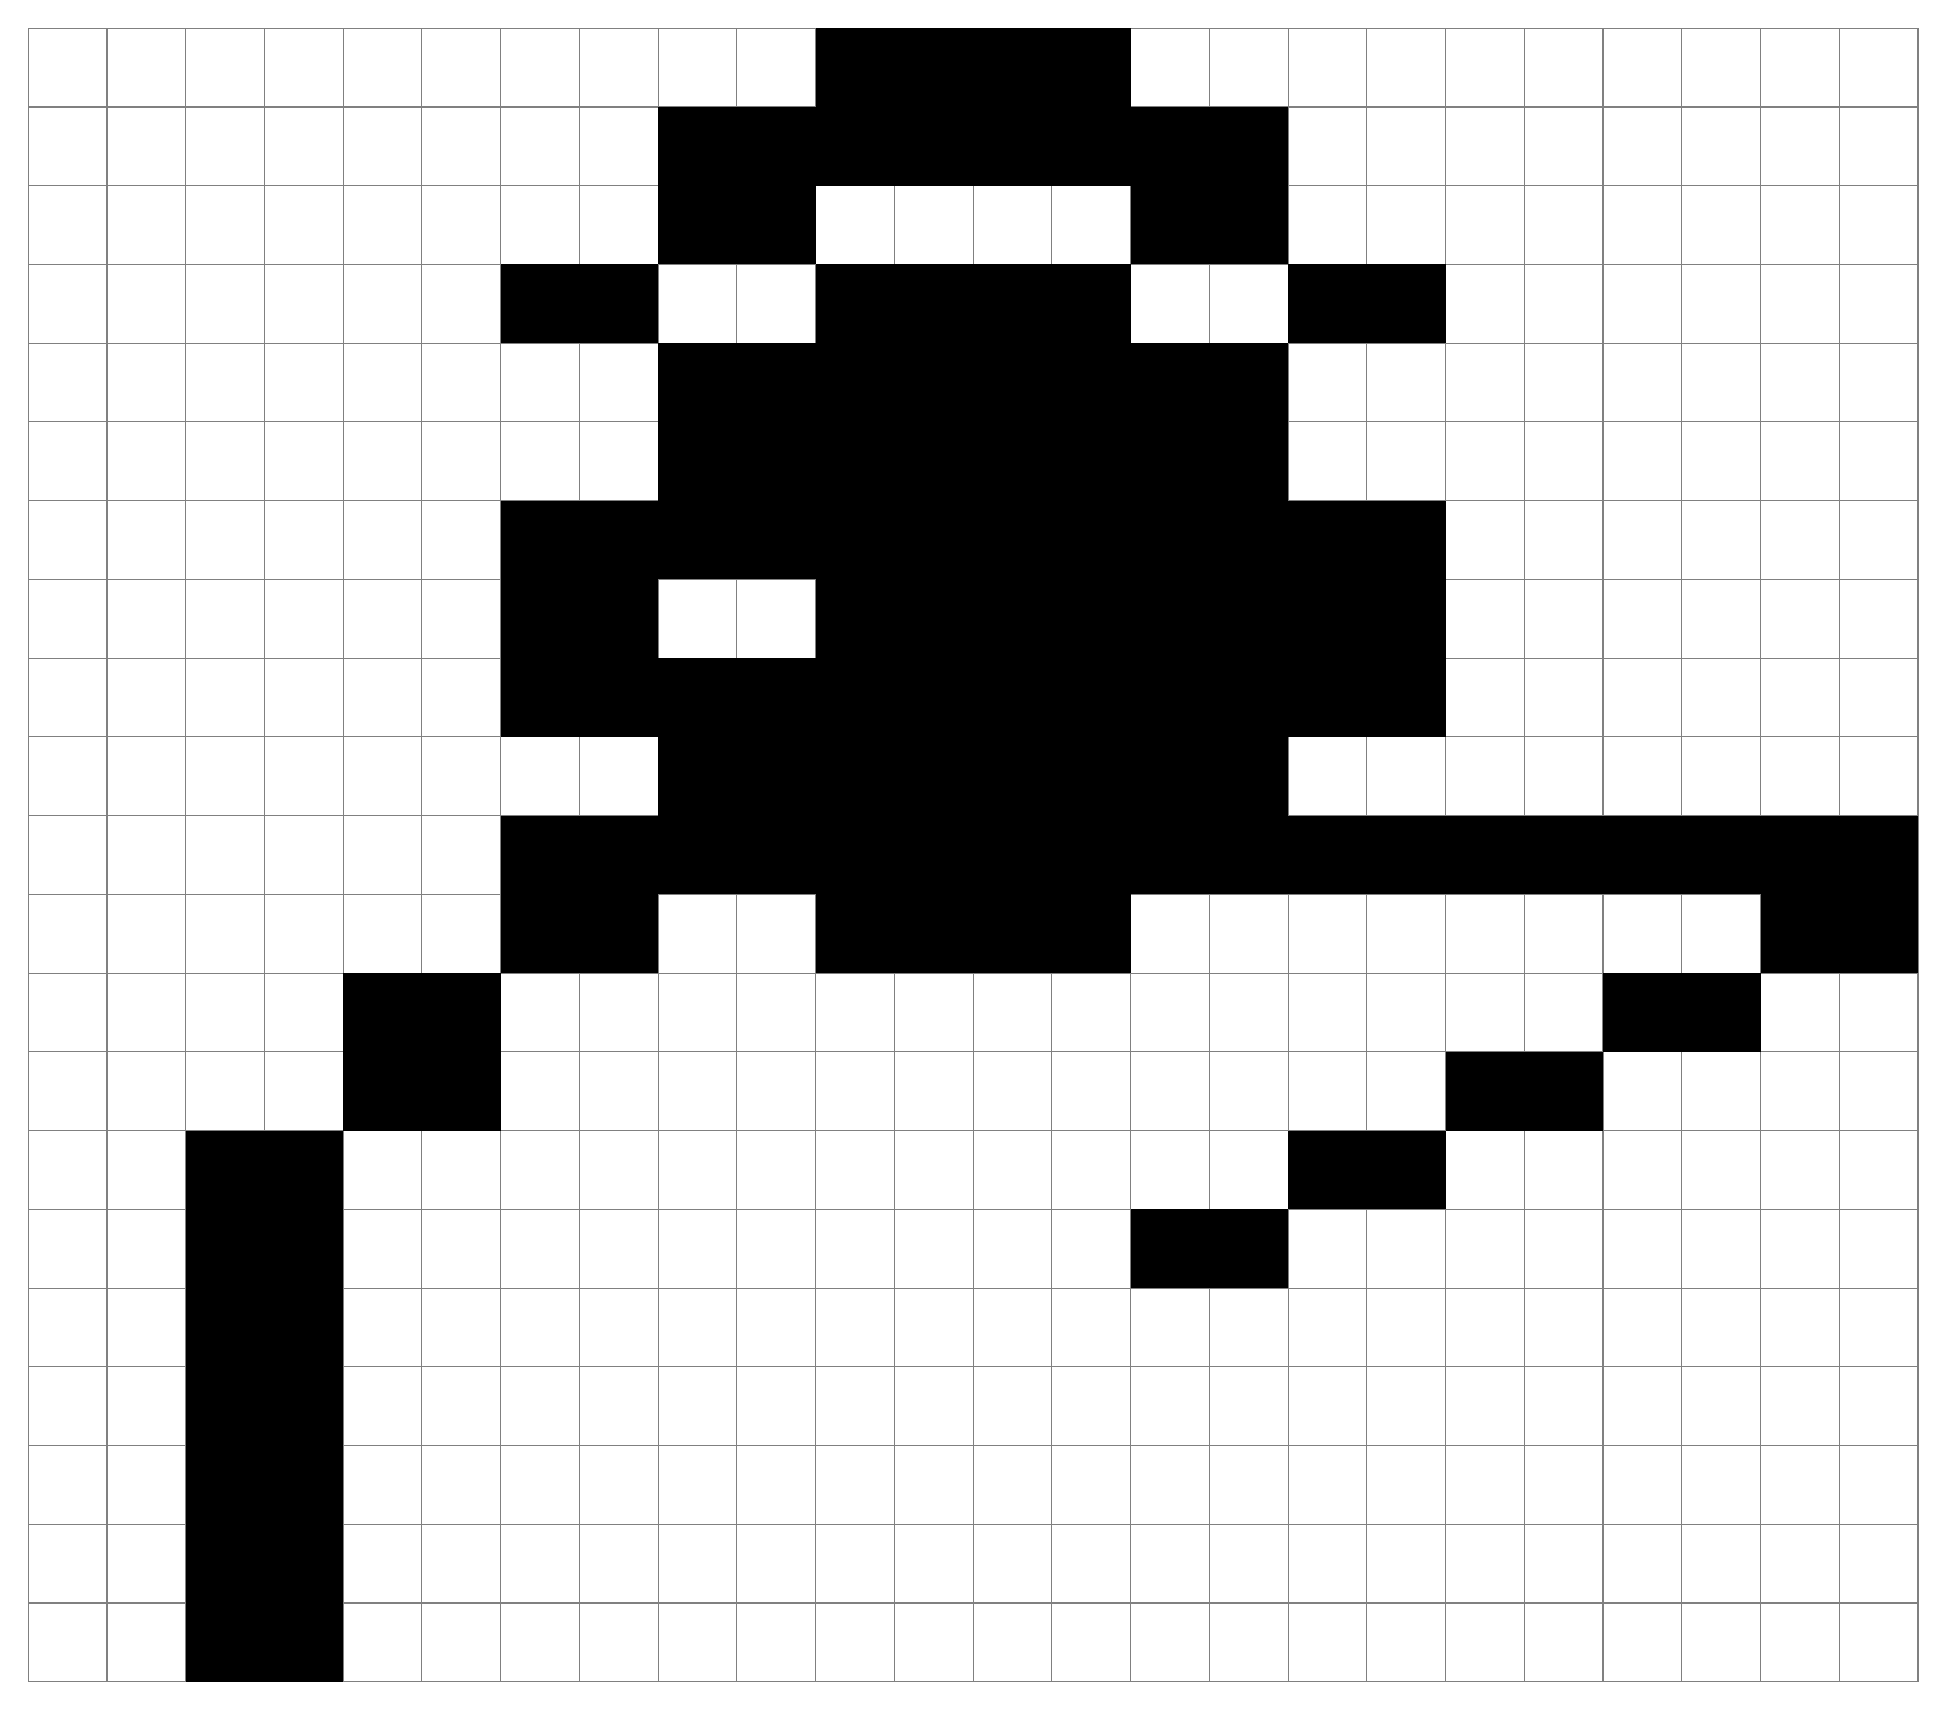
\begin{tikzpicture}

	\draw[step=1.0,gray,thin] (0,0) grid (24,21);
	\fill[\SPRITECOLOR] (10,20) rectangle ++ (1,1);
	\fill[\SPRITECOLOR] (11,20) rectangle ++ (1,1);
	\fill[\SPRITECOLOR] (12,20) rectangle ++ (1,1);
	\fill[\SPRITECOLOR] (13,20) rectangle ++ (1,1);
	\fill[\SPRITECOLOR] (8,19) rectangle ++ (1,1);
	\fill[\SPRITECOLOR] (9,19) rectangle ++ (1,1);
	\fill[\SPRITECOLOR] (10,19) rectangle ++ (1,1);
	\fill[\SPRITECOLOR] (11,19) rectangle ++ (1,1);
	\fill[\SPRITECOLOR] (12,19) rectangle ++ (1,1);
	\fill[\SPRITECOLOR] (13,19) rectangle ++ (1,1);
	\fill[\SPRITECOLOR] (14,19) rectangle ++ (1,1);
	\fill[\SPRITECOLOR] (15,19) rectangle ++ (1,1);
	\fill[\SPRITECOLOR] (8,18) rectangle ++ (1,1);
	\fill[\SPRITECOLOR] (9,18) rectangle ++ (1,1);
	\fill[\SPRITECOLOR] (14,18) rectangle ++ (1,1);
	\fill[\SPRITECOLOR] (15,18) rectangle ++ (1,1);
	\fill[\SPRITECOLOR] (6,17) rectangle ++ (1,1);
	\fill[\SPRITECOLOR] (7,17) rectangle ++ (1,1);
	\fill[\SPRITECOLOR] (10,17) rectangle ++ (1,1);
	\fill[\SPRITECOLOR] (11,17) rectangle ++ (1,1);
	\fill[\SPRITECOLOR] (12,17) rectangle ++ (1,1);
	\fill[\SPRITECOLOR] (13,17) rectangle ++ (1,1);
	\fill[\SPRITECOLOR] (16,17) rectangle ++ (1,1);
	\fill[\SPRITECOLOR] (17,17) rectangle ++ (1,1);
	\fill[\SPRITECOLOR] (8,16) rectangle ++ (1,1);
	\fill[\SPRITECOLOR] (9,16) rectangle ++ (1,1);
	\fill[\MULTICOLORTWO] (10,16) rectangle ++ (1,1);
	\fill[\MULTICOLORTWO] (11,16) rectangle ++ (1,1);
	\fill[\SPRITECOLOR] (12,16) rectangle ++ (1,1);
	\fill[\SPRITECOLOR] (13,16) rectangle ++ (1,1);
	\fill[\SPRITECOLOR] (14,16) rectangle ++ (1,1);
	\fill[\SPRITECOLOR] (15,16) rectangle ++ (1,1);
	\fill[\MULTICOLORTWO] (8,15) rectangle ++ (1,1);
	\fill[\MULTICOLORTWO] (9,15) rectangle ++ (1,1);
	\fill[\SPRITECOLOR] (10,15) rectangle ++ (1,1);
	\fill[\SPRITECOLOR] (11,15) rectangle ++ (1,1);
	\fill[\SPRITECOLOR] (12,15) rectangle ++ (1,1);
	\fill[\SPRITECOLOR] (13,15) rectangle ++ (1,1);
	\fill[\SPRITECOLOR] (14,15) rectangle ++ (1,1);
	\fill[\SPRITECOLOR] (15,15) rectangle ++ (1,1);
	\fill[\MULTICOLORTWO] (6,14) rectangle ++ (1,1);
	\fill[\MULTICOLORTWO] (7,14) rectangle ++ (1,1);
	\fill[\MULTICOLORTWO] (8,14) rectangle ++ (1,1);
	\fill[\MULTICOLORTWO] (9,14) rectangle ++ (1,1);
	\fill[\MULTICOLORTWO] (10,14) rectangle ++ (1,1);
	\fill[\MULTICOLORTWO] (11,14) rectangle ++ (1,1);
	\fill[\SPRITECOLOR] (12,14) rectangle ++ (1,1);
	\fill[\SPRITECOLOR] (13,14) rectangle ++ (1,1);
	\fill[\SPRITECOLOR] (14,14) rectangle ++ (1,1);
	\fill[\SPRITECOLOR] (15,14) rectangle ++ (1,1);
	\fill[\SPRITECOLOR] (16,14) rectangle ++ (1,1);
	\fill[\SPRITECOLOR] (17,14) rectangle ++ (1,1);
	\fill[\MULTICOLORTWO] (6,13) rectangle ++ (1,1);
	\fill[\MULTICOLORTWO] (7,13) rectangle ++ (1,1);
	\fill[\MULTICOLORTWO] (10,13) rectangle ++ (1,1);
	\fill[\MULTICOLORTWO] (11,13) rectangle ++ (1,1);
	\fill[\SPRITECOLOR] (12,13) rectangle ++ (1,1);
	\fill[\SPRITECOLOR] (13,13) rectangle ++ (1,1);
	\fill[\SPRITECOLOR] (14,13) rectangle ++ (1,1);
	\fill[\SPRITECOLOR] (15,13) rectangle ++ (1,1);
	\fill[\SPRITECOLOR] (16,13) rectangle ++ (1,1);
	\fill[\SPRITECOLOR] (17,13) rectangle ++ (1,1);
	\fill[\MULTICOLORTWO] (6,12) rectangle ++ (1,1);
	\fill[\MULTICOLORTWO] (7,12) rectangle ++ (1,1);
	\fill[\MULTICOLORTWO] (8,12) rectangle ++ (1,1);
	\fill[\MULTICOLORTWO] (9,12) rectangle ++ (1,1);
	\fill[\MULTICOLORTWO] (10,12) rectangle ++ (1,1);
	\fill[\MULTICOLORTWO] (11,12) rectangle ++ (1,1);
	\fill[\SPRITECOLOR] (12,12) rectangle ++ (1,1);
	\fill[\SPRITECOLOR] (13,12) rectangle ++ (1,1);
	\fill[\SPRITECOLOR] (14,12) rectangle ++ (1,1);
	\fill[\SPRITECOLOR] (15,12) rectangle ++ (1,1);
	\fill[\SPRITECOLOR] (16,12) rectangle ++ (1,1);
	\fill[\SPRITECOLOR] (17,12) rectangle ++ (1,1);
	\fill[\SPRITECOLOR] (8,11) rectangle ++ (1,1);
	\fill[\SPRITECOLOR] (9,11) rectangle ++ (1,1);
	\fill[\SPRITECOLOR] (10,11) rectangle ++ (1,1);
	\fill[\SPRITECOLOR] (11,11) rectangle ++ (1,1);
	\fill[\SPRITECOLOR] (12,11) rectangle ++ (1,1);
	\fill[\SPRITECOLOR] (13,11) rectangle ++ (1,1);
	\fill[\SPRITECOLOR] (14,11) rectangle ++ (1,1);
	\fill[\SPRITECOLOR] (15,11) rectangle ++ (1,1);
	\fill[\MULTICOLORONE] (6,10) rectangle ++ (1,1);
	\fill[\MULTICOLORONE] (7,10) rectangle ++ (1,1);
	\fill[\SPRITECOLOR] (8,10) rectangle ++ (1,1);
	\fill[\SPRITECOLOR] (9,10) rectangle ++ (1,1);
	\fill[\SPRITECOLOR] (10,10) rectangle ++ (1,1);
	\fill[\SPRITECOLOR] (11,10) rectangle ++ (1,1);
	\fill[\SPRITECOLOR] (12,10) rectangle ++ (1,1);
	\fill[\SPRITECOLOR] (13,10) rectangle ++ (1,1);
	\fill[\SPRITECOLOR] (14,10) rectangle ++ (1,1);
	\fill[\SPRITECOLOR] (15,10) rectangle ++ (1,1);
	\fill[\MULTICOLORONE] (16,10) rectangle ++ (1,1);
	\fill[\MULTICOLORONE] (17,10) rectangle ++ (1,1);
	\fill[\MULTICOLORONE] (18,10) rectangle ++ (1,1);
	\fill[\MULTICOLORONE] (19,10) rectangle ++ (1,1);
	\fill[\MULTICOLORONE] (20,10) rectangle ++ (1,1);
	\fill[\MULTICOLORONE] (21,10) rectangle ++ (1,1);
	\fill[\MULTICOLORTWO] (22,10) rectangle ++ (1,1);
	\fill[\MULTICOLORTWO] (23,10) rectangle ++ (1,1);
	\fill[\MULTICOLORONE] (6,9) rectangle ++ (1,1);
	\fill[\MULTICOLORONE] (7,9) rectangle ++ (1,1);
	\fill[\SPRITECOLOR] (10,9) rectangle ++ (1,1);
	\fill[\SPRITECOLOR] (11,9) rectangle ++ (1,1);
	\fill[\SPRITECOLOR] (12,9) rectangle ++ (1,1);
	\fill[\SPRITECOLOR] (13,9) rectangle ++ (1,1);
	\fill[\MULTICOLORONE] (22,9) rectangle ++ (1,1);
	\fill[\MULTICOLORONE] (23,9) rectangle ++ (1,1);
	\fill[\MULTICOLORONE] (4,8) rectangle ++ (1,1);
	\fill[\MULTICOLORONE] (5,8) rectangle ++ (1,1);
	\fill[\MULTICOLORONE] (20,8) rectangle ++ (1,1);
	\fill[\MULTICOLORONE] (21,8) rectangle ++ (1,1);
	\fill[\MULTICOLORONE] (4,7) rectangle ++ (1,1);
	\fill[\MULTICOLORONE] (5,7) rectangle ++ (1,1);
	\fill[\MULTICOLORONE] (18,7) rectangle ++ (1,1);
	\fill[\MULTICOLORONE] (19,7) rectangle ++ (1,1);
	\fill[\MULTICOLORTWO] (2,6) rectangle ++ (1,1);
	\fill[\MULTICOLORTWO] (3,6) rectangle ++ (1,1);
	\fill[\MULTICOLORONE] (16,6) rectangle ++ (1,1);
	\fill[\MULTICOLORONE] (17,6) rectangle ++ (1,1);
	\fill[\MULTICOLORONE] (2,5) rectangle ++ (1,1);
	\fill[\MULTICOLORONE] (3,5) rectangle ++ (1,1);
	\fill[\MULTICOLORONE] (14,5) rectangle ++ (1,1);
	\fill[\MULTICOLORONE] (15,5) rectangle ++ (1,1);
	\fill[\MULTICOLORONE] (2,4) rectangle ++ (1,1);
	\fill[\MULTICOLORONE] (3,4) rectangle ++ (1,1);
	\fill[\MULTICOLORONE] (2,3) rectangle ++ (1,1);
	\fill[\MULTICOLORONE] (3,3) rectangle ++ (1,1);
	\fill[\MULTICOLORONE] (2,2) rectangle ++ (1,1);
	\fill[\MULTICOLORONE] (3,2) rectangle ++ (1,1);
	\fill[\MULTICOLORONE] (2,1) rectangle ++ (1,1);
	\fill[\MULTICOLORONE] (3,1) rectangle ++ (1,1);
	\fill[\MULTICOLORONE] (2,0) rectangle ++ (1,1);
	\fill[\MULTICOLORONE] (3,0) rectangle ++ (1,1);

      \end{tikzpicture}
    \end{adjustbox}
  }\caption{LAND\_GILBY2}
\end{figure}

	\end{subfigure}
} & 
\makecell[l]{
	\begin{subfigure}{0.3\textwidth}
    \def\MULTICOLORONE{gray}
    \def\MULTICOLORTWO{white}
    \def\SPRITECOLOR{orange}
		
\begin{figure}[H]
  {
    \setlength{\tabcolsep}{3.0pt}
    \setlength\cmidrulewidth{\heavyrulewidth} % Make cmidrule = 
    \begin{adjustbox}{width=3cm,center}
      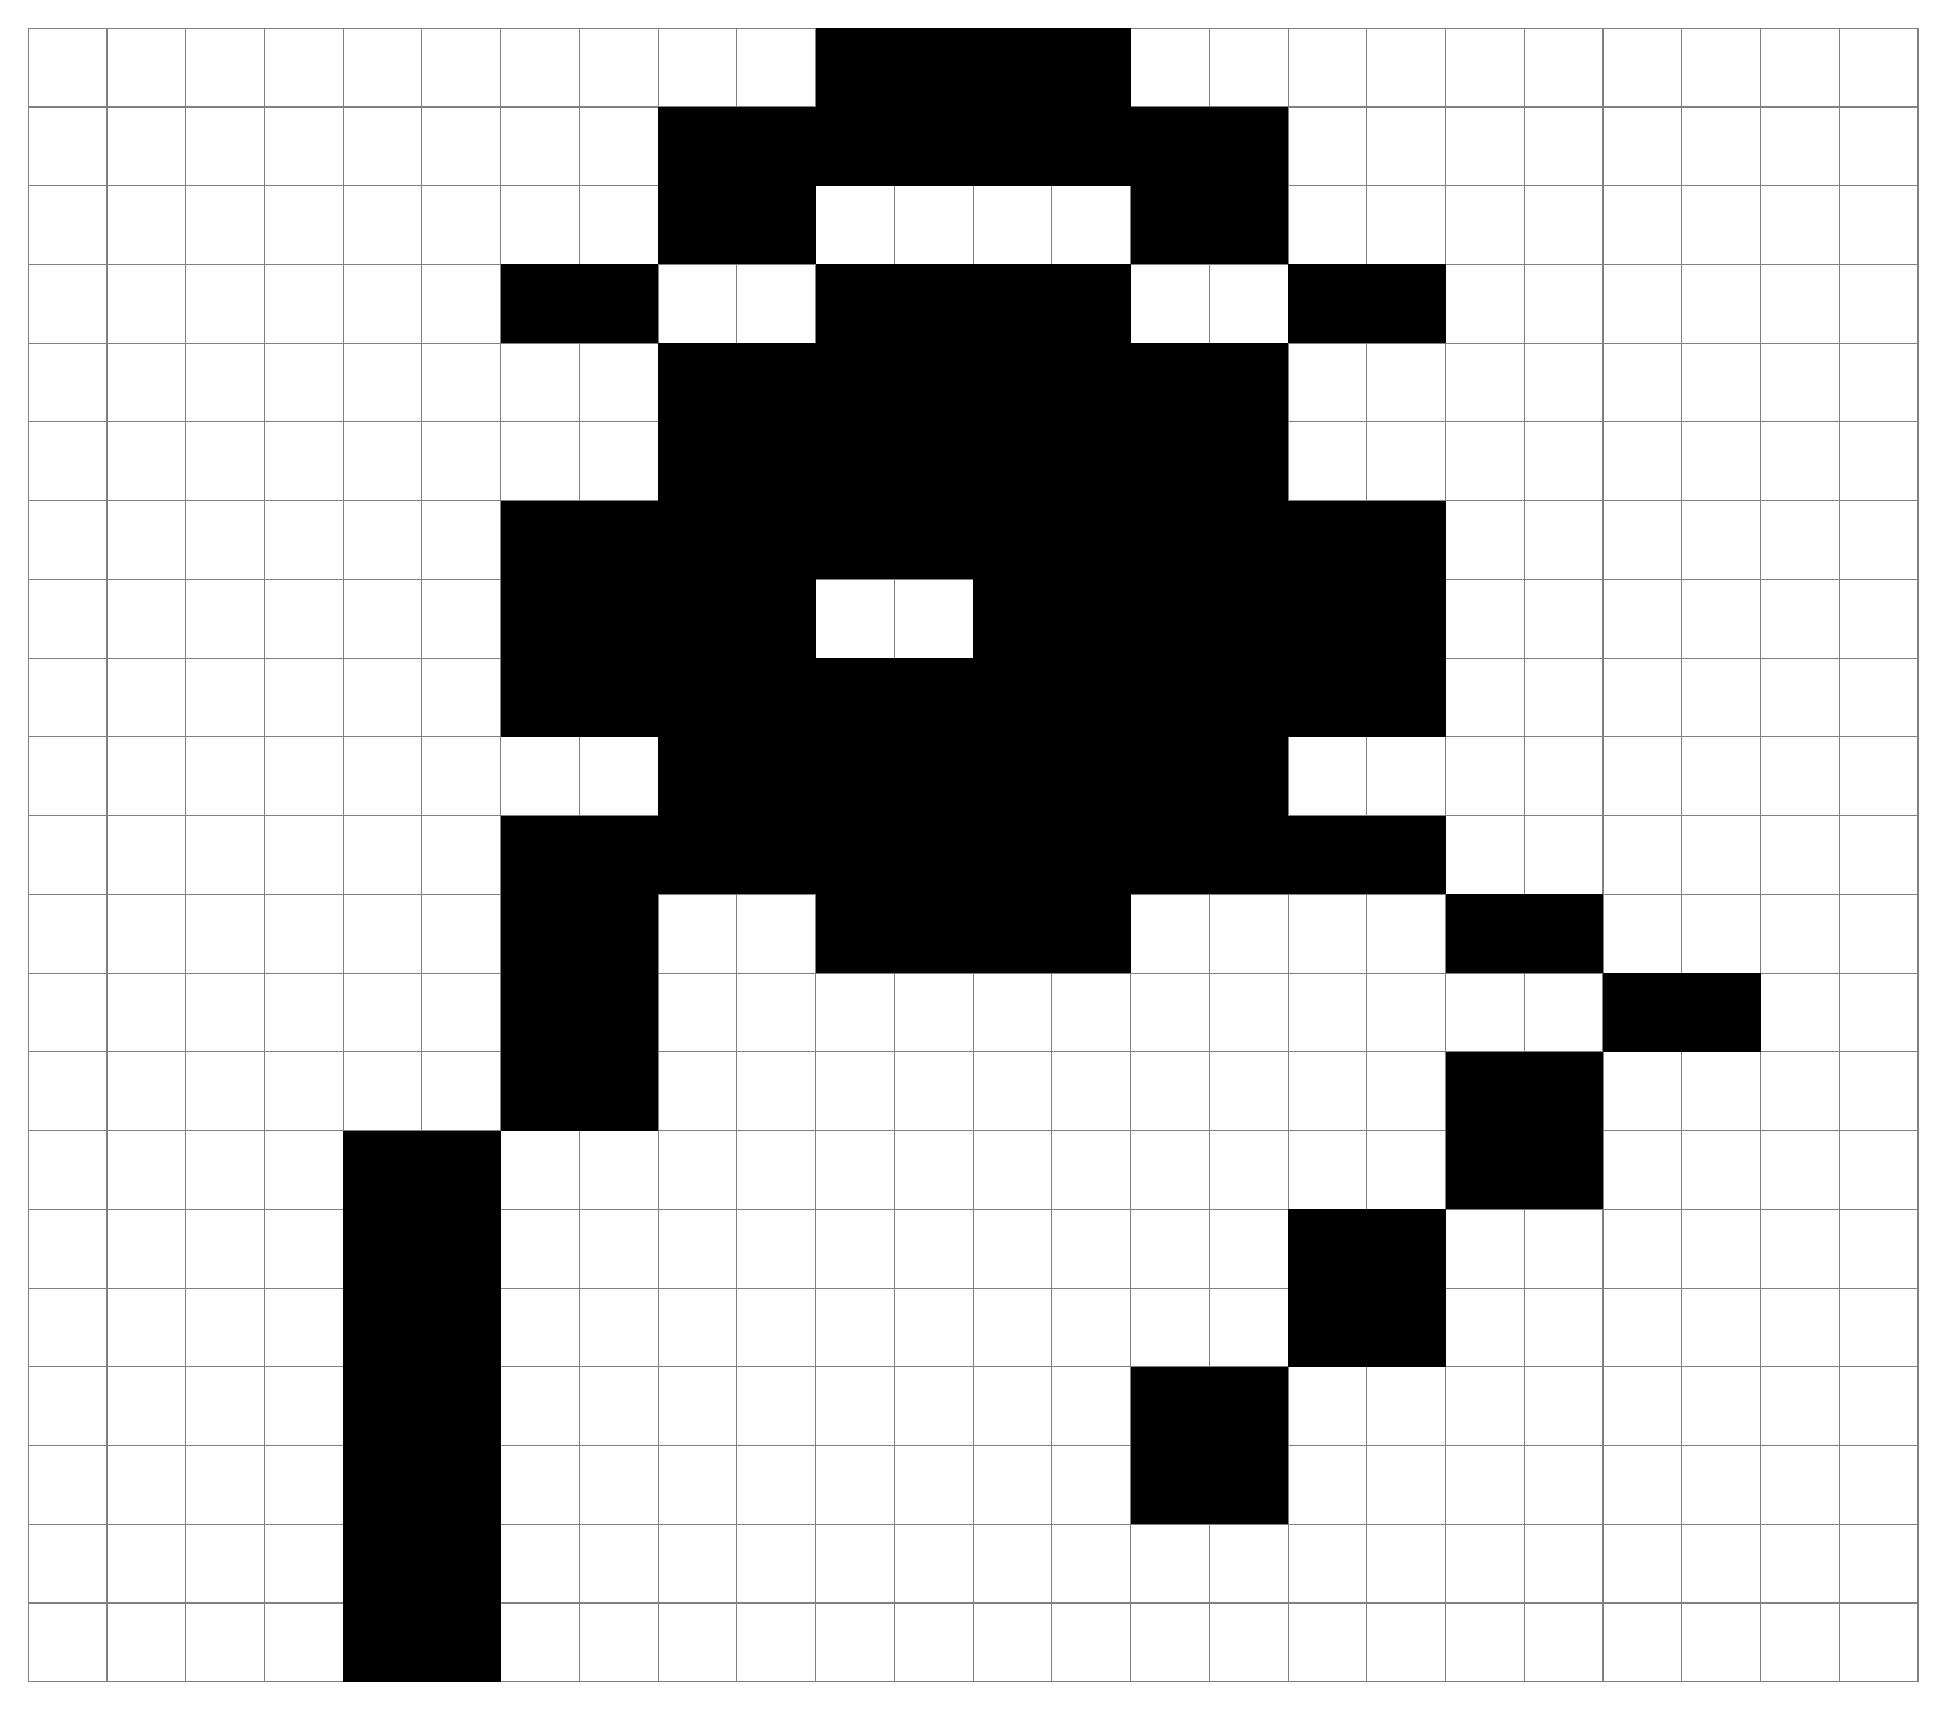
\begin{tikzpicture}

	\draw[step=1.0,gray,thin] (0,0) grid (24,21);
	\fill[\SPRITECOLOR] (10,20) rectangle ++ (1,1);
	\fill[\SPRITECOLOR] (11,20) rectangle ++ (1,1);
	\fill[\SPRITECOLOR] (12,20) rectangle ++ (1,1);
	\fill[\SPRITECOLOR] (13,20) rectangle ++ (1,1);
	\fill[\SPRITECOLOR] (8,19) rectangle ++ (1,1);
	\fill[\SPRITECOLOR] (9,19) rectangle ++ (1,1);
	\fill[\SPRITECOLOR] (10,19) rectangle ++ (1,1);
	\fill[\SPRITECOLOR] (11,19) rectangle ++ (1,1);
	\fill[\SPRITECOLOR] (12,19) rectangle ++ (1,1);
	\fill[\SPRITECOLOR] (13,19) rectangle ++ (1,1);
	\fill[\SPRITECOLOR] (14,19) rectangle ++ (1,1);
	\fill[\SPRITECOLOR] (15,19) rectangle ++ (1,1);
	\fill[\SPRITECOLOR] (8,18) rectangle ++ (1,1);
	\fill[\SPRITECOLOR] (9,18) rectangle ++ (1,1);
	\fill[\SPRITECOLOR] (14,18) rectangle ++ (1,1);
	\fill[\SPRITECOLOR] (15,18) rectangle ++ (1,1);
	\fill[\SPRITECOLOR] (6,17) rectangle ++ (1,1);
	\fill[\SPRITECOLOR] (7,17) rectangle ++ (1,1);
	\fill[\SPRITECOLOR] (10,17) rectangle ++ (1,1);
	\fill[\SPRITECOLOR] (11,17) rectangle ++ (1,1);
	\fill[\SPRITECOLOR] (12,17) rectangle ++ (1,1);
	\fill[\SPRITECOLOR] (13,17) rectangle ++ (1,1);
	\fill[\SPRITECOLOR] (16,17) rectangle ++ (1,1);
	\fill[\SPRITECOLOR] (17,17) rectangle ++ (1,1);
	\fill[\SPRITECOLOR] (8,16) rectangle ++ (1,1);
	\fill[\SPRITECOLOR] (9,16) rectangle ++ (1,1);
	\fill[\MULTICOLORTWO] (10,16) rectangle ++ (1,1);
	\fill[\MULTICOLORTWO] (11,16) rectangle ++ (1,1);
	\fill[\SPRITECOLOR] (12,16) rectangle ++ (1,1);
	\fill[\SPRITECOLOR] (13,16) rectangle ++ (1,1);
	\fill[\SPRITECOLOR] (14,16) rectangle ++ (1,1);
	\fill[\SPRITECOLOR] (15,16) rectangle ++ (1,1);
	\fill[\MULTICOLORTWO] (8,15) rectangle ++ (1,1);
	\fill[\MULTICOLORTWO] (9,15) rectangle ++ (1,1);
	\fill[\SPRITECOLOR] (10,15) rectangle ++ (1,1);
	\fill[\SPRITECOLOR] (11,15) rectangle ++ (1,1);
	\fill[\SPRITECOLOR] (12,15) rectangle ++ (1,1);
	\fill[\SPRITECOLOR] (13,15) rectangle ++ (1,1);
	\fill[\SPRITECOLOR] (14,15) rectangle ++ (1,1);
	\fill[\SPRITECOLOR] (15,15) rectangle ++ (1,1);
	\fill[\SPRITECOLOR] (6,14) rectangle ++ (1,1);
	\fill[\SPRITECOLOR] (7,14) rectangle ++ (1,1);
	\fill[\MULTICOLORTWO] (8,14) rectangle ++ (1,1);
	\fill[\MULTICOLORTWO] (9,14) rectangle ++ (1,1);
	\fill[\MULTICOLORTWO] (10,14) rectangle ++ (1,1);
	\fill[\MULTICOLORTWO] (11,14) rectangle ++ (1,1);
	\fill[\MULTICOLORTWO] (12,14) rectangle ++ (1,1);
	\fill[\MULTICOLORTWO] (13,14) rectangle ++ (1,1);
	\fill[\SPRITECOLOR] (14,14) rectangle ++ (1,1);
	\fill[\SPRITECOLOR] (15,14) rectangle ++ (1,1);
	\fill[\SPRITECOLOR] (16,14) rectangle ++ (1,1);
	\fill[\SPRITECOLOR] (17,14) rectangle ++ (1,1);
	\fill[\SPRITECOLOR] (6,13) rectangle ++ (1,1);
	\fill[\SPRITECOLOR] (7,13) rectangle ++ (1,1);
	\fill[\MULTICOLORTWO] (8,13) rectangle ++ (1,1);
	\fill[\MULTICOLORTWO] (9,13) rectangle ++ (1,1);
	\fill[\MULTICOLORTWO] (12,13) rectangle ++ (1,1);
	\fill[\MULTICOLORTWO] (13,13) rectangle ++ (1,1);
	\fill[\SPRITECOLOR] (14,13) rectangle ++ (1,1);
	\fill[\SPRITECOLOR] (15,13) rectangle ++ (1,1);
	\fill[\SPRITECOLOR] (16,13) rectangle ++ (1,1);
	\fill[\SPRITECOLOR] (17,13) rectangle ++ (1,1);
	\fill[\SPRITECOLOR] (6,12) rectangle ++ (1,1);
	\fill[\SPRITECOLOR] (7,12) rectangle ++ (1,1);
	\fill[\MULTICOLORTWO] (8,12) rectangle ++ (1,1);
	\fill[\MULTICOLORTWO] (9,12) rectangle ++ (1,1);
	\fill[\MULTICOLORTWO] (10,12) rectangle ++ (1,1);
	\fill[\MULTICOLORTWO] (11,12) rectangle ++ (1,1);
	\fill[\MULTICOLORTWO] (12,12) rectangle ++ (1,1);
	\fill[\MULTICOLORTWO] (13,12) rectangle ++ (1,1);
	\fill[\SPRITECOLOR] (14,12) rectangle ++ (1,1);
	\fill[\SPRITECOLOR] (15,12) rectangle ++ (1,1);
	\fill[\SPRITECOLOR] (16,12) rectangle ++ (1,1);
	\fill[\SPRITECOLOR] (17,12) rectangle ++ (1,1);
	\fill[\SPRITECOLOR] (8,11) rectangle ++ (1,1);
	\fill[\SPRITECOLOR] (9,11) rectangle ++ (1,1);
	\fill[\SPRITECOLOR] (10,11) rectangle ++ (1,1);
	\fill[\SPRITECOLOR] (11,11) rectangle ++ (1,1);
	\fill[\SPRITECOLOR] (12,11) rectangle ++ (1,1);
	\fill[\SPRITECOLOR] (13,11) rectangle ++ (1,1);
	\fill[\SPRITECOLOR] (14,11) rectangle ++ (1,1);
	\fill[\SPRITECOLOR] (15,11) rectangle ++ (1,1);
	\fill[\MULTICOLORONE] (6,10) rectangle ++ (1,1);
	\fill[\MULTICOLORONE] (7,10) rectangle ++ (1,1);
	\fill[\SPRITECOLOR] (8,10) rectangle ++ (1,1);
	\fill[\SPRITECOLOR] (9,10) rectangle ++ (1,1);
	\fill[\SPRITECOLOR] (10,10) rectangle ++ (1,1);
	\fill[\SPRITECOLOR] (11,10) rectangle ++ (1,1);
	\fill[\SPRITECOLOR] (12,10) rectangle ++ (1,1);
	\fill[\SPRITECOLOR] (13,10) rectangle ++ (1,1);
	\fill[\SPRITECOLOR] (14,10) rectangle ++ (1,1);
	\fill[\SPRITECOLOR] (15,10) rectangle ++ (1,1);
	\fill[\MULTICOLORONE] (16,10) rectangle ++ (1,1);
	\fill[\MULTICOLORONE] (17,10) rectangle ++ (1,1);
	\fill[\MULTICOLORONE] (6,9) rectangle ++ (1,1);
	\fill[\MULTICOLORONE] (7,9) rectangle ++ (1,1);
	\fill[\SPRITECOLOR] (10,9) rectangle ++ (1,1);
	\fill[\SPRITECOLOR] (11,9) rectangle ++ (1,1);
	\fill[\SPRITECOLOR] (12,9) rectangle ++ (1,1);
	\fill[\SPRITECOLOR] (13,9) rectangle ++ (1,1);
	\fill[\MULTICOLORONE] (18,9) rectangle ++ (1,1);
	\fill[\MULTICOLORONE] (19,9) rectangle ++ (1,1);
	\fill[\MULTICOLORONE] (6,8) rectangle ++ (1,1);
	\fill[\MULTICOLORONE] (7,8) rectangle ++ (1,1);
	\fill[\MULTICOLORTWO] (20,8) rectangle ++ (1,1);
	\fill[\MULTICOLORTWO] (21,8) rectangle ++ (1,1);
	\fill[\MULTICOLORONE] (6,7) rectangle ++ (1,1);
	\fill[\MULTICOLORONE] (7,7) rectangle ++ (1,1);
	\fill[\MULTICOLORONE] (18,7) rectangle ++ (1,1);
	\fill[\MULTICOLORONE] (19,7) rectangle ++ (1,1);
	\fill[\MULTICOLORTWO] (4,6) rectangle ++ (1,1);
	\fill[\MULTICOLORTWO] (5,6) rectangle ++ (1,1);
	\fill[\MULTICOLORONE] (18,6) rectangle ++ (1,1);
	\fill[\MULTICOLORONE] (19,6) rectangle ++ (1,1);
	\fill[\MULTICOLORONE] (4,5) rectangle ++ (1,1);
	\fill[\MULTICOLORONE] (5,5) rectangle ++ (1,1);
	\fill[\MULTICOLORONE] (16,5) rectangle ++ (1,1);
	\fill[\MULTICOLORONE] (17,5) rectangle ++ (1,1);
	\fill[\MULTICOLORONE] (4,4) rectangle ++ (1,1);
	\fill[\MULTICOLORONE] (5,4) rectangle ++ (1,1);
	\fill[\MULTICOLORONE] (16,4) rectangle ++ (1,1);
	\fill[\MULTICOLORONE] (17,4) rectangle ++ (1,1);
	\fill[\MULTICOLORONE] (4,3) rectangle ++ (1,1);
	\fill[\MULTICOLORONE] (5,3) rectangle ++ (1,1);
	\fill[\MULTICOLORONE] (14,3) rectangle ++ (1,1);
	\fill[\MULTICOLORONE] (15,3) rectangle ++ (1,1);
	\fill[\MULTICOLORONE] (4,2) rectangle ++ (1,1);
	\fill[\MULTICOLORONE] (5,2) rectangle ++ (1,1);
	\fill[\MULTICOLORONE] (14,2) rectangle ++ (1,1);
	\fill[\MULTICOLORONE] (15,2) rectangle ++ (1,1);
	\fill[\MULTICOLORONE] (4,1) rectangle ++ (1,1);
	\fill[\MULTICOLORONE] (5,1) rectangle ++ (1,1);
	\fill[\MULTICOLORONE] (4,0) rectangle ++ (1,1);
	\fill[\MULTICOLORONE] (5,0) rectangle ++ (1,1);

      \end{tikzpicture}
    \end{adjustbox}
  }\caption{LAND\_GILBY3}
\end{figure}

	\end{subfigure}
} & 
\makecell[l]{
	\begin{subfigure}{0.3\textwidth}
    \def\MULTICOLORONE{gray}
    \def\MULTICOLORTWO{white}
    \def\SPRITECOLOR{yellow}
		
\begin{figure}[H]
  {
    \setlength{\tabcolsep}{3.0pt}
    \setlength\cmidrulewidth{\heavyrulewidth} % Make cmidrule = 
    \begin{adjustbox}{width=3cm,center}
      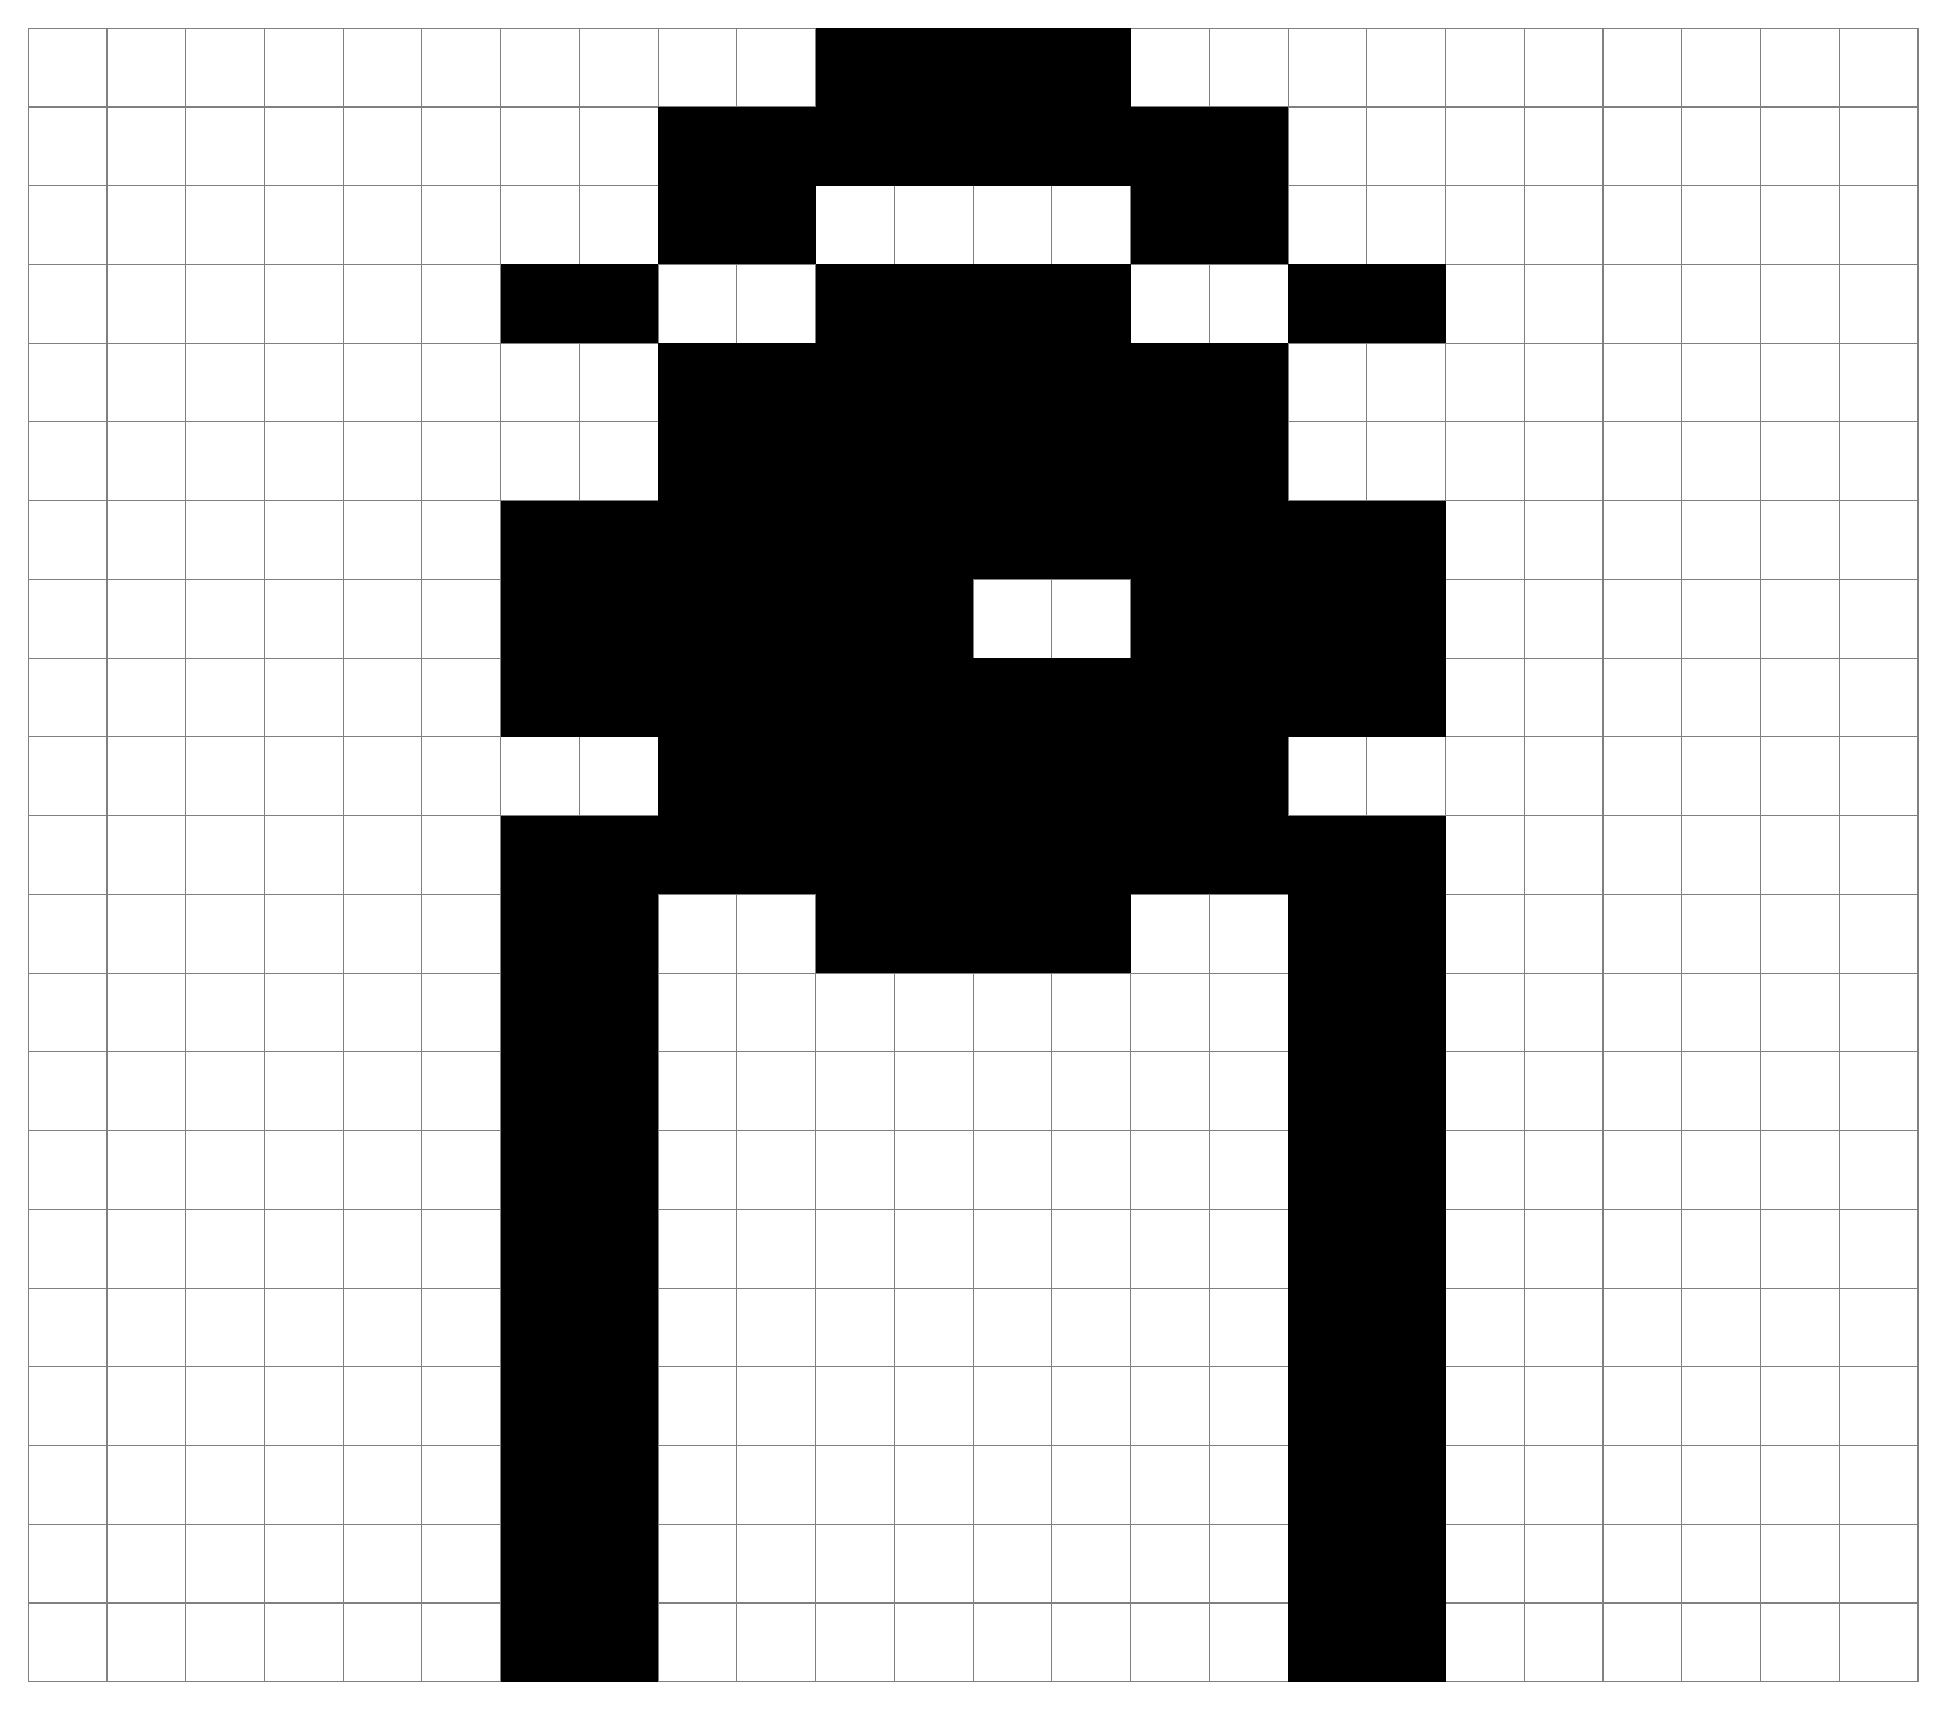
\begin{tikzpicture}

	\draw[step=1.0,gray,thin] (0,0) grid (24,21);
	\fill[\SPRITECOLOR] (10,20) rectangle ++ (1,1);
	\fill[\SPRITECOLOR] (11,20) rectangle ++ (1,1);
	\fill[\SPRITECOLOR] (12,20) rectangle ++ (1,1);
	\fill[\SPRITECOLOR] (13,20) rectangle ++ (1,1);
	\fill[\SPRITECOLOR] (8,19) rectangle ++ (1,1);
	\fill[\SPRITECOLOR] (9,19) rectangle ++ (1,1);
	\fill[\SPRITECOLOR] (10,19) rectangle ++ (1,1);
	\fill[\SPRITECOLOR] (11,19) rectangle ++ (1,1);
	\fill[\SPRITECOLOR] (12,19) rectangle ++ (1,1);
	\fill[\SPRITECOLOR] (13,19) rectangle ++ (1,1);
	\fill[\SPRITECOLOR] (14,19) rectangle ++ (1,1);
	\fill[\SPRITECOLOR] (15,19) rectangle ++ (1,1);
	\fill[\SPRITECOLOR] (8,18) rectangle ++ (1,1);
	\fill[\SPRITECOLOR] (9,18) rectangle ++ (1,1);
	\fill[\SPRITECOLOR] (14,18) rectangle ++ (1,1);
	\fill[\SPRITECOLOR] (15,18) rectangle ++ (1,1);
	\fill[\SPRITECOLOR] (6,17) rectangle ++ (1,1);
	\fill[\SPRITECOLOR] (7,17) rectangle ++ (1,1);
	\fill[\SPRITECOLOR] (10,17) rectangle ++ (1,1);
	\fill[\SPRITECOLOR] (11,17) rectangle ++ (1,1);
	\fill[\SPRITECOLOR] (12,17) rectangle ++ (1,1);
	\fill[\SPRITECOLOR] (13,17) rectangle ++ (1,1);
	\fill[\SPRITECOLOR] (16,17) rectangle ++ (1,1);
	\fill[\SPRITECOLOR] (17,17) rectangle ++ (1,1);
	\fill[\SPRITECOLOR] (8,16) rectangle ++ (1,1);
	\fill[\SPRITECOLOR] (9,16) rectangle ++ (1,1);
	\fill[\MULTICOLORTWO] (10,16) rectangle ++ (1,1);
	\fill[\MULTICOLORTWO] (11,16) rectangle ++ (1,1);
	\fill[\SPRITECOLOR] (12,16) rectangle ++ (1,1);
	\fill[\SPRITECOLOR] (13,16) rectangle ++ (1,1);
	\fill[\SPRITECOLOR] (14,16) rectangle ++ (1,1);
	\fill[\SPRITECOLOR] (15,16) rectangle ++ (1,1);
	\fill[\MULTICOLORTWO] (8,15) rectangle ++ (1,1);
	\fill[\MULTICOLORTWO] (9,15) rectangle ++ (1,1);
	\fill[\SPRITECOLOR] (10,15) rectangle ++ (1,1);
	\fill[\SPRITECOLOR] (11,15) rectangle ++ (1,1);
	\fill[\SPRITECOLOR] (12,15) rectangle ++ (1,1);
	\fill[\SPRITECOLOR] (13,15) rectangle ++ (1,1);
	\fill[\SPRITECOLOR] (14,15) rectangle ++ (1,1);
	\fill[\SPRITECOLOR] (15,15) rectangle ++ (1,1);
	\fill[\SPRITECOLOR] (6,14) rectangle ++ (1,1);
	\fill[\SPRITECOLOR] (7,14) rectangle ++ (1,1);
	\fill[\SPRITECOLOR] (8,14) rectangle ++ (1,1);
	\fill[\SPRITECOLOR] (9,14) rectangle ++ (1,1);
	\fill[\MULTICOLORTWO] (10,14) rectangle ++ (1,1);
	\fill[\MULTICOLORTWO] (11,14) rectangle ++ (1,1);
	\fill[\MULTICOLORTWO] (12,14) rectangle ++ (1,1);
	\fill[\MULTICOLORTWO] (13,14) rectangle ++ (1,1);
	\fill[\MULTICOLORTWO] (14,14) rectangle ++ (1,1);
	\fill[\MULTICOLORTWO] (15,14) rectangle ++ (1,1);
	\fill[\SPRITECOLOR] (16,14) rectangle ++ (1,1);
	\fill[\SPRITECOLOR] (17,14) rectangle ++ (1,1);
	\fill[\SPRITECOLOR] (6,13) rectangle ++ (1,1);
	\fill[\SPRITECOLOR] (7,13) rectangle ++ (1,1);
	\fill[\SPRITECOLOR] (8,13) rectangle ++ (1,1);
	\fill[\SPRITECOLOR] (9,13) rectangle ++ (1,1);
	\fill[\MULTICOLORTWO] (10,13) rectangle ++ (1,1);
	\fill[\MULTICOLORTWO] (11,13) rectangle ++ (1,1);
	\fill[\MULTICOLORTWO] (14,13) rectangle ++ (1,1);
	\fill[\MULTICOLORTWO] (15,13) rectangle ++ (1,1);
	\fill[\SPRITECOLOR] (16,13) rectangle ++ (1,1);
	\fill[\SPRITECOLOR] (17,13) rectangle ++ (1,1);
	\fill[\SPRITECOLOR] (6,12) rectangle ++ (1,1);
	\fill[\SPRITECOLOR] (7,12) rectangle ++ (1,1);
	\fill[\SPRITECOLOR] (8,12) rectangle ++ (1,1);
	\fill[\SPRITECOLOR] (9,12) rectangle ++ (1,1);
	\fill[\MULTICOLORTWO] (10,12) rectangle ++ (1,1);
	\fill[\MULTICOLORTWO] (11,12) rectangle ++ (1,1);
	\fill[\MULTICOLORTWO] (12,12) rectangle ++ (1,1);
	\fill[\MULTICOLORTWO] (13,12) rectangle ++ (1,1);
	\fill[\MULTICOLORTWO] (14,12) rectangle ++ (1,1);
	\fill[\MULTICOLORTWO] (15,12) rectangle ++ (1,1);
	\fill[\SPRITECOLOR] (16,12) rectangle ++ (1,1);
	\fill[\SPRITECOLOR] (17,12) rectangle ++ (1,1);
	\fill[\SPRITECOLOR] (8,11) rectangle ++ (1,1);
	\fill[\SPRITECOLOR] (9,11) rectangle ++ (1,1);
	\fill[\SPRITECOLOR] (10,11) rectangle ++ (1,1);
	\fill[\SPRITECOLOR] (11,11) rectangle ++ (1,1);
	\fill[\SPRITECOLOR] (12,11) rectangle ++ (1,1);
	\fill[\SPRITECOLOR] (13,11) rectangle ++ (1,1);
	\fill[\SPRITECOLOR] (14,11) rectangle ++ (1,1);
	\fill[\SPRITECOLOR] (15,11) rectangle ++ (1,1);
	\fill[\MULTICOLORONE] (6,10) rectangle ++ (1,1);
	\fill[\MULTICOLORONE] (7,10) rectangle ++ (1,1);
	\fill[\SPRITECOLOR] (8,10) rectangle ++ (1,1);
	\fill[\SPRITECOLOR] (9,10) rectangle ++ (1,1);
	\fill[\SPRITECOLOR] (10,10) rectangle ++ (1,1);
	\fill[\SPRITECOLOR] (11,10) rectangle ++ (1,1);
	\fill[\SPRITECOLOR] (12,10) rectangle ++ (1,1);
	\fill[\SPRITECOLOR] (13,10) rectangle ++ (1,1);
	\fill[\SPRITECOLOR] (14,10) rectangle ++ (1,1);
	\fill[\SPRITECOLOR] (15,10) rectangle ++ (1,1);
	\fill[\MULTICOLORONE] (16,10) rectangle ++ (1,1);
	\fill[\MULTICOLORONE] (17,10) rectangle ++ (1,1);
	\fill[\MULTICOLORONE] (6,9) rectangle ++ (1,1);
	\fill[\MULTICOLORONE] (7,9) rectangle ++ (1,1);
	\fill[\SPRITECOLOR] (10,9) rectangle ++ (1,1);
	\fill[\SPRITECOLOR] (11,9) rectangle ++ (1,1);
	\fill[\SPRITECOLOR] (12,9) rectangle ++ (1,1);
	\fill[\SPRITECOLOR] (13,9) rectangle ++ (1,1);
	\fill[\MULTICOLORONE] (16,9) rectangle ++ (1,1);
	\fill[\MULTICOLORONE] (17,9) rectangle ++ (1,1);
	\fill[\MULTICOLORONE] (6,8) rectangle ++ (1,1);
	\fill[\MULTICOLORONE] (7,8) rectangle ++ (1,1);
	\fill[\MULTICOLORONE] (16,8) rectangle ++ (1,1);
	\fill[\MULTICOLORONE] (17,8) rectangle ++ (1,1);
	\fill[\MULTICOLORONE] (6,7) rectangle ++ (1,1);
	\fill[\MULTICOLORONE] (7,7) rectangle ++ (1,1);
	\fill[\MULTICOLORONE] (16,7) rectangle ++ (1,1);
	\fill[\MULTICOLORONE] (17,7) rectangle ++ (1,1);
	\fill[\MULTICOLORTWO] (6,6) rectangle ++ (1,1);
	\fill[\MULTICOLORTWO] (7,6) rectangle ++ (1,1);
	\fill[\MULTICOLORTWO] (16,6) rectangle ++ (1,1);
	\fill[\MULTICOLORTWO] (17,6) rectangle ++ (1,1);
	\fill[\MULTICOLORONE] (6,5) rectangle ++ (1,1);
	\fill[\MULTICOLORONE] (7,5) rectangle ++ (1,1);
	\fill[\MULTICOLORONE] (16,5) rectangle ++ (1,1);
	\fill[\MULTICOLORONE] (17,5) rectangle ++ (1,1);
	\fill[\MULTICOLORONE] (6,4) rectangle ++ (1,1);
	\fill[\MULTICOLORONE] (7,4) rectangle ++ (1,1);
	\fill[\MULTICOLORONE] (16,4) rectangle ++ (1,1);
	\fill[\MULTICOLORONE] (17,4) rectangle ++ (1,1);
	\fill[\MULTICOLORONE] (6,3) rectangle ++ (1,1);
	\fill[\MULTICOLORONE] (7,3) rectangle ++ (1,1);
	\fill[\MULTICOLORONE] (16,3) rectangle ++ (1,1);
	\fill[\MULTICOLORONE] (17,3) rectangle ++ (1,1);
	\fill[\MULTICOLORONE] (6,2) rectangle ++ (1,1);
	\fill[\MULTICOLORONE] (7,2) rectangle ++ (1,1);
	\fill[\MULTICOLORONE] (16,2) rectangle ++ (1,1);
	\fill[\MULTICOLORONE] (17,2) rectangle ++ (1,1);
	\fill[\MULTICOLORONE] (6,1) rectangle ++ (1,1);
	\fill[\MULTICOLORONE] (7,1) rectangle ++ (1,1);
	\fill[\MULTICOLORONE] (16,1) rectangle ++ (1,1);
	\fill[\MULTICOLORONE] (17,1) rectangle ++ (1,1);
	\fill[\MULTICOLORONE] (6,0) rectangle ++ (1,1);
	\fill[\MULTICOLORONE] (7,0) rectangle ++ (1,1);
	\fill[\MULTICOLORONE] (16,0) rectangle ++ (1,1);
	\fill[\MULTICOLORONE] (17,0) rectangle ++ (1,1);

      \end{tikzpicture}
    \end{adjustbox}
  }\caption{LAND\_GILBY4}
\end{figure}

	\end{subfigure}
} & 
\makecell[l]{
	\begin{subfigure}{0.3\textwidth}
    \def\MULTICOLORONE{gray}
    \def\MULTICOLORTWO{white}
    \def\SPRITECOLOR{green}
		
\begin{figure}[H]
  {
    \setlength{\tabcolsep}{3.0pt}
    \setlength\cmidrulewidth{\heavyrulewidth} % Make cmidrule = 
    \begin{adjustbox}{width=3cm,center}
      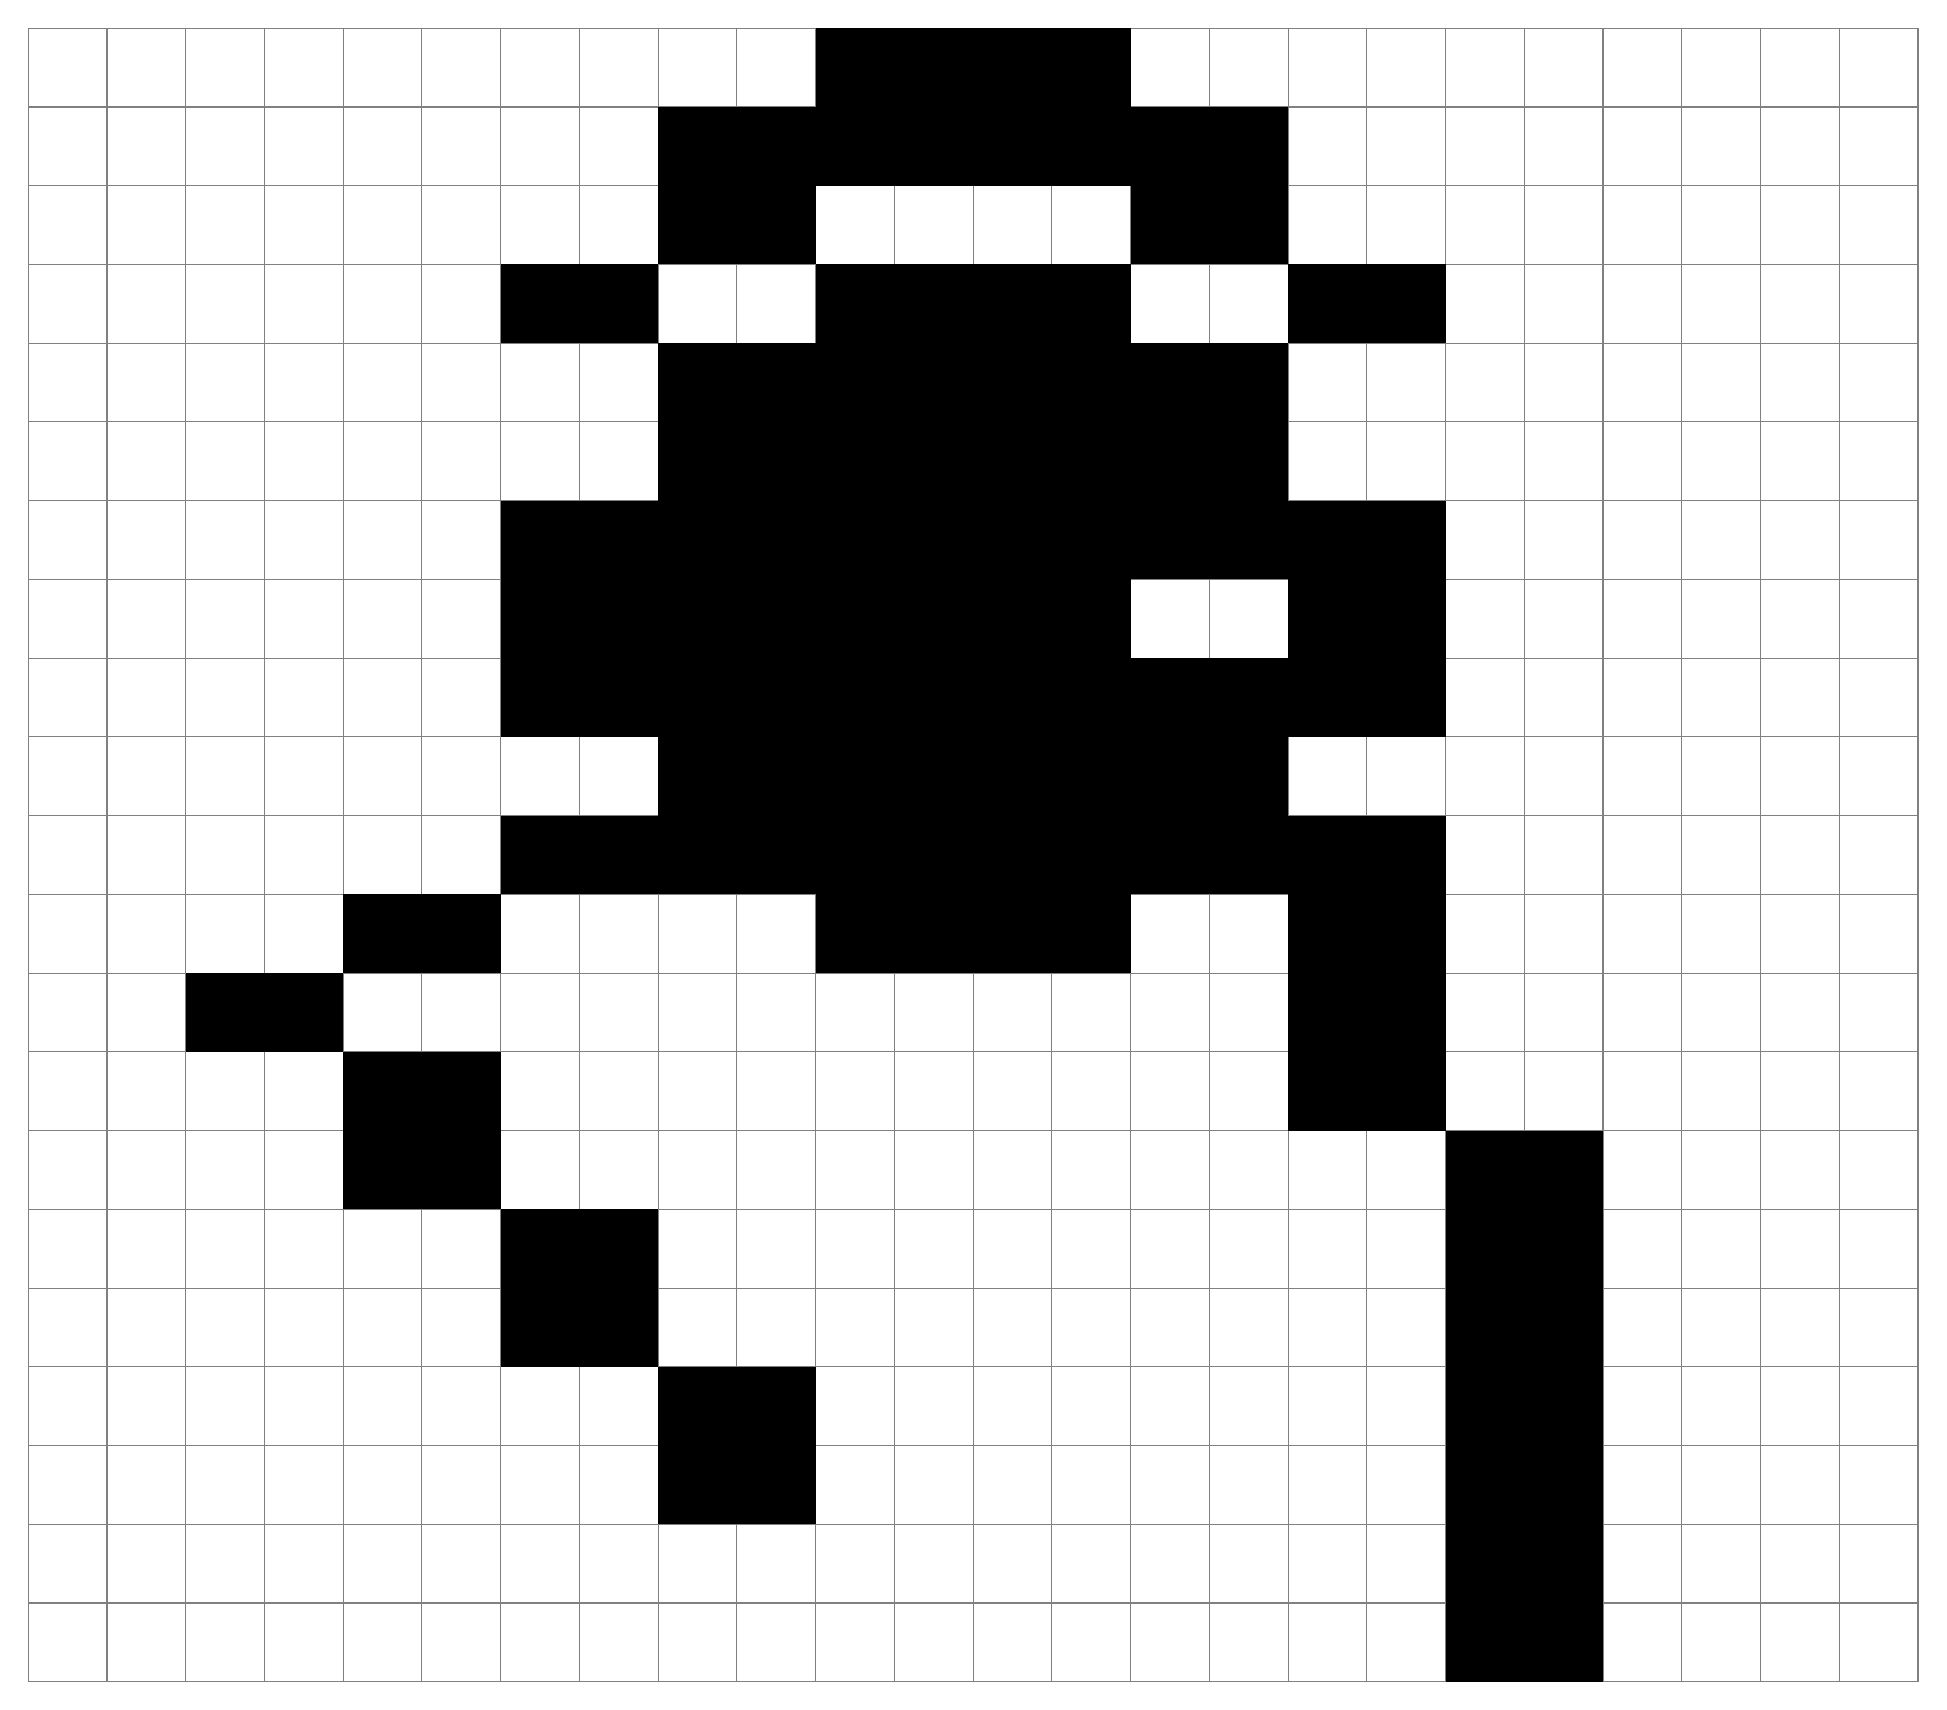
\begin{tikzpicture}

	\draw[step=1.0,gray,thin] (0,0) grid (24,21);
	\fill[\SPRITECOLOR] (10,20) rectangle ++ (1,1);
	\fill[\SPRITECOLOR] (11,20) rectangle ++ (1,1);
	\fill[\SPRITECOLOR] (12,20) rectangle ++ (1,1);
	\fill[\SPRITECOLOR] (13,20) rectangle ++ (1,1);
	\fill[\SPRITECOLOR] (8,19) rectangle ++ (1,1);
	\fill[\SPRITECOLOR] (9,19) rectangle ++ (1,1);
	\fill[\SPRITECOLOR] (10,19) rectangle ++ (1,1);
	\fill[\SPRITECOLOR] (11,19) rectangle ++ (1,1);
	\fill[\SPRITECOLOR] (12,19) rectangle ++ (1,1);
	\fill[\SPRITECOLOR] (13,19) rectangle ++ (1,1);
	\fill[\SPRITECOLOR] (14,19) rectangle ++ (1,1);
	\fill[\SPRITECOLOR] (15,19) rectangle ++ (1,1);
	\fill[\SPRITECOLOR] (8,18) rectangle ++ (1,1);
	\fill[\SPRITECOLOR] (9,18) rectangle ++ (1,1);
	\fill[\SPRITECOLOR] (14,18) rectangle ++ (1,1);
	\fill[\SPRITECOLOR] (15,18) rectangle ++ (1,1);
	\fill[\SPRITECOLOR] (6,17) rectangle ++ (1,1);
	\fill[\SPRITECOLOR] (7,17) rectangle ++ (1,1);
	\fill[\SPRITECOLOR] (10,17) rectangle ++ (1,1);
	\fill[\SPRITECOLOR] (11,17) rectangle ++ (1,1);
	\fill[\SPRITECOLOR] (12,17) rectangle ++ (1,1);
	\fill[\SPRITECOLOR] (13,17) rectangle ++ (1,1);
	\fill[\SPRITECOLOR] (16,17) rectangle ++ (1,1);
	\fill[\SPRITECOLOR] (17,17) rectangle ++ (1,1);
	\fill[\SPRITECOLOR] (8,16) rectangle ++ (1,1);
	\fill[\SPRITECOLOR] (9,16) rectangle ++ (1,1);
	\fill[\MULTICOLORTWO] (10,16) rectangle ++ (1,1);
	\fill[\MULTICOLORTWO] (11,16) rectangle ++ (1,1);
	\fill[\SPRITECOLOR] (12,16) rectangle ++ (1,1);
	\fill[\SPRITECOLOR] (13,16) rectangle ++ (1,1);
	\fill[\SPRITECOLOR] (14,16) rectangle ++ (1,1);
	\fill[\SPRITECOLOR] (15,16) rectangle ++ (1,1);
	\fill[\MULTICOLORTWO] (8,15) rectangle ++ (1,1);
	\fill[\MULTICOLORTWO] (9,15) rectangle ++ (1,1);
	\fill[\SPRITECOLOR] (10,15) rectangle ++ (1,1);
	\fill[\SPRITECOLOR] (11,15) rectangle ++ (1,1);
	\fill[\SPRITECOLOR] (12,15) rectangle ++ (1,1);
	\fill[\SPRITECOLOR] (13,15) rectangle ++ (1,1);
	\fill[\SPRITECOLOR] (14,15) rectangle ++ (1,1);
	\fill[\SPRITECOLOR] (15,15) rectangle ++ (1,1);
	\fill[\SPRITECOLOR] (6,14) rectangle ++ (1,1);
	\fill[\SPRITECOLOR] (7,14) rectangle ++ (1,1);
	\fill[\SPRITECOLOR] (8,14) rectangle ++ (1,1);
	\fill[\SPRITECOLOR] (9,14) rectangle ++ (1,1);
	\fill[\SPRITECOLOR] (10,14) rectangle ++ (1,1);
	\fill[\SPRITECOLOR] (11,14) rectangle ++ (1,1);
	\fill[\MULTICOLORTWO] (12,14) rectangle ++ (1,1);
	\fill[\MULTICOLORTWO] (13,14) rectangle ++ (1,1);
	\fill[\MULTICOLORTWO] (14,14) rectangle ++ (1,1);
	\fill[\MULTICOLORTWO] (15,14) rectangle ++ (1,1);
	\fill[\MULTICOLORTWO] (16,14) rectangle ++ (1,1);
	\fill[\MULTICOLORTWO] (17,14) rectangle ++ (1,1);
	\fill[\SPRITECOLOR] (6,13) rectangle ++ (1,1);
	\fill[\SPRITECOLOR] (7,13) rectangle ++ (1,1);
	\fill[\SPRITECOLOR] (8,13) rectangle ++ (1,1);
	\fill[\SPRITECOLOR] (9,13) rectangle ++ (1,1);
	\fill[\SPRITECOLOR] (10,13) rectangle ++ (1,1);
	\fill[\SPRITECOLOR] (11,13) rectangle ++ (1,1);
	\fill[\MULTICOLORTWO] (12,13) rectangle ++ (1,1);
	\fill[\MULTICOLORTWO] (13,13) rectangle ++ (1,1);
	\fill[\MULTICOLORTWO] (16,13) rectangle ++ (1,1);
	\fill[\MULTICOLORTWO] (17,13) rectangle ++ (1,1);
	\fill[\SPRITECOLOR] (6,12) rectangle ++ (1,1);
	\fill[\SPRITECOLOR] (7,12) rectangle ++ (1,1);
	\fill[\SPRITECOLOR] (8,12) rectangle ++ (1,1);
	\fill[\SPRITECOLOR] (9,12) rectangle ++ (1,1);
	\fill[\SPRITECOLOR] (10,12) rectangle ++ (1,1);
	\fill[\SPRITECOLOR] (11,12) rectangle ++ (1,1);
	\fill[\MULTICOLORTWO] (12,12) rectangle ++ (1,1);
	\fill[\MULTICOLORTWO] (13,12) rectangle ++ (1,1);
	\fill[\MULTICOLORTWO] (14,12) rectangle ++ (1,1);
	\fill[\MULTICOLORTWO] (15,12) rectangle ++ (1,1);
	\fill[\MULTICOLORTWO] (16,12) rectangle ++ (1,1);
	\fill[\MULTICOLORTWO] (17,12) rectangle ++ (1,1);
	\fill[\SPRITECOLOR] (8,11) rectangle ++ (1,1);
	\fill[\SPRITECOLOR] (9,11) rectangle ++ (1,1);
	\fill[\SPRITECOLOR] (10,11) rectangle ++ (1,1);
	\fill[\SPRITECOLOR] (11,11) rectangle ++ (1,1);
	\fill[\SPRITECOLOR] (12,11) rectangle ++ (1,1);
	\fill[\SPRITECOLOR] (13,11) rectangle ++ (1,1);
	\fill[\SPRITECOLOR] (14,11) rectangle ++ (1,1);
	\fill[\SPRITECOLOR] (15,11) rectangle ++ (1,1);
	\fill[\MULTICOLORONE] (6,10) rectangle ++ (1,1);
	\fill[\MULTICOLORONE] (7,10) rectangle ++ (1,1);
	\fill[\SPRITECOLOR] (8,10) rectangle ++ (1,1);
	\fill[\SPRITECOLOR] (9,10) rectangle ++ (1,1);
	\fill[\SPRITECOLOR] (10,10) rectangle ++ (1,1);
	\fill[\SPRITECOLOR] (11,10) rectangle ++ (1,1);
	\fill[\SPRITECOLOR] (12,10) rectangle ++ (1,1);
	\fill[\SPRITECOLOR] (13,10) rectangle ++ (1,1);
	\fill[\SPRITECOLOR] (14,10) rectangle ++ (1,1);
	\fill[\SPRITECOLOR] (15,10) rectangle ++ (1,1);
	\fill[\MULTICOLORONE] (16,10) rectangle ++ (1,1);
	\fill[\MULTICOLORONE] (17,10) rectangle ++ (1,1);
	\fill[\MULTICOLORONE] (4,9) rectangle ++ (1,1);
	\fill[\MULTICOLORONE] (5,9) rectangle ++ (1,1);
	\fill[\SPRITECOLOR] (10,9) rectangle ++ (1,1);
	\fill[\SPRITECOLOR] (11,9) rectangle ++ (1,1);
	\fill[\SPRITECOLOR] (12,9) rectangle ++ (1,1);
	\fill[\SPRITECOLOR] (13,9) rectangle ++ (1,1);
	\fill[\MULTICOLORONE] (16,9) rectangle ++ (1,1);
	\fill[\MULTICOLORONE] (17,9) rectangle ++ (1,1);
	\fill[\MULTICOLORTWO] (2,8) rectangle ++ (1,1);
	\fill[\MULTICOLORTWO] (3,8) rectangle ++ (1,1);
	\fill[\MULTICOLORONE] (16,8) rectangle ++ (1,1);
	\fill[\MULTICOLORONE] (17,8) rectangle ++ (1,1);
	\fill[\MULTICOLORONE] (4,7) rectangle ++ (1,1);
	\fill[\MULTICOLORONE] (5,7) rectangle ++ (1,1);
	\fill[\MULTICOLORONE] (16,7) rectangle ++ (1,1);
	\fill[\MULTICOLORONE] (17,7) rectangle ++ (1,1);
	\fill[\MULTICOLORONE] (4,6) rectangle ++ (1,1);
	\fill[\MULTICOLORONE] (5,6) rectangle ++ (1,1);
	\fill[\MULTICOLORTWO] (18,6) rectangle ++ (1,1);
	\fill[\MULTICOLORTWO] (19,6) rectangle ++ (1,1);
	\fill[\MULTICOLORONE] (6,5) rectangle ++ (1,1);
	\fill[\MULTICOLORONE] (7,5) rectangle ++ (1,1);
	\fill[\MULTICOLORONE] (18,5) rectangle ++ (1,1);
	\fill[\MULTICOLORONE] (19,5) rectangle ++ (1,1);
	\fill[\MULTICOLORONE] (6,4) rectangle ++ (1,1);
	\fill[\MULTICOLORONE] (7,4) rectangle ++ (1,1);
	\fill[\MULTICOLORONE] (18,4) rectangle ++ (1,1);
	\fill[\MULTICOLORONE] (19,4) rectangle ++ (1,1);
	\fill[\MULTICOLORONE] (8,3) rectangle ++ (1,1);
	\fill[\MULTICOLORONE] (9,3) rectangle ++ (1,1);
	\fill[\MULTICOLORONE] (18,3) rectangle ++ (1,1);
	\fill[\MULTICOLORONE] (19,3) rectangle ++ (1,1);
	\fill[\MULTICOLORONE] (8,2) rectangle ++ (1,1);
	\fill[\MULTICOLORONE] (9,2) rectangle ++ (1,1);
	\fill[\MULTICOLORONE] (18,2) rectangle ++ (1,1);
	\fill[\MULTICOLORONE] (19,2) rectangle ++ (1,1);
	\fill[\MULTICOLORONE] (18,1) rectangle ++ (1,1);
	\fill[\MULTICOLORONE] (19,1) rectangle ++ (1,1);
	\fill[\MULTICOLORONE] (18,0) rectangle ++ (1,1);
	\fill[\MULTICOLORONE] (19,0) rectangle ++ (1,1);

      \end{tikzpicture}
    \end{adjustbox}
  }\caption{LAND\_GILBY5}
\end{figure}

	\end{subfigure}
} & 
\makecell[l]{
	\begin{subfigure}{0.3\textwidth}
    \def\MULTICOLORONE{gray}
    \def\MULTICOLORTWO{white}
    \def\SPRITECOLOR{lightblue}
		
\begin{figure}[H]
  {
    \setlength{\tabcolsep}{3.0pt}
    \setlength\cmidrulewidth{\heavyrulewidth} % Make cmidrule = 
    \begin{adjustbox}{width=3cm,center}
      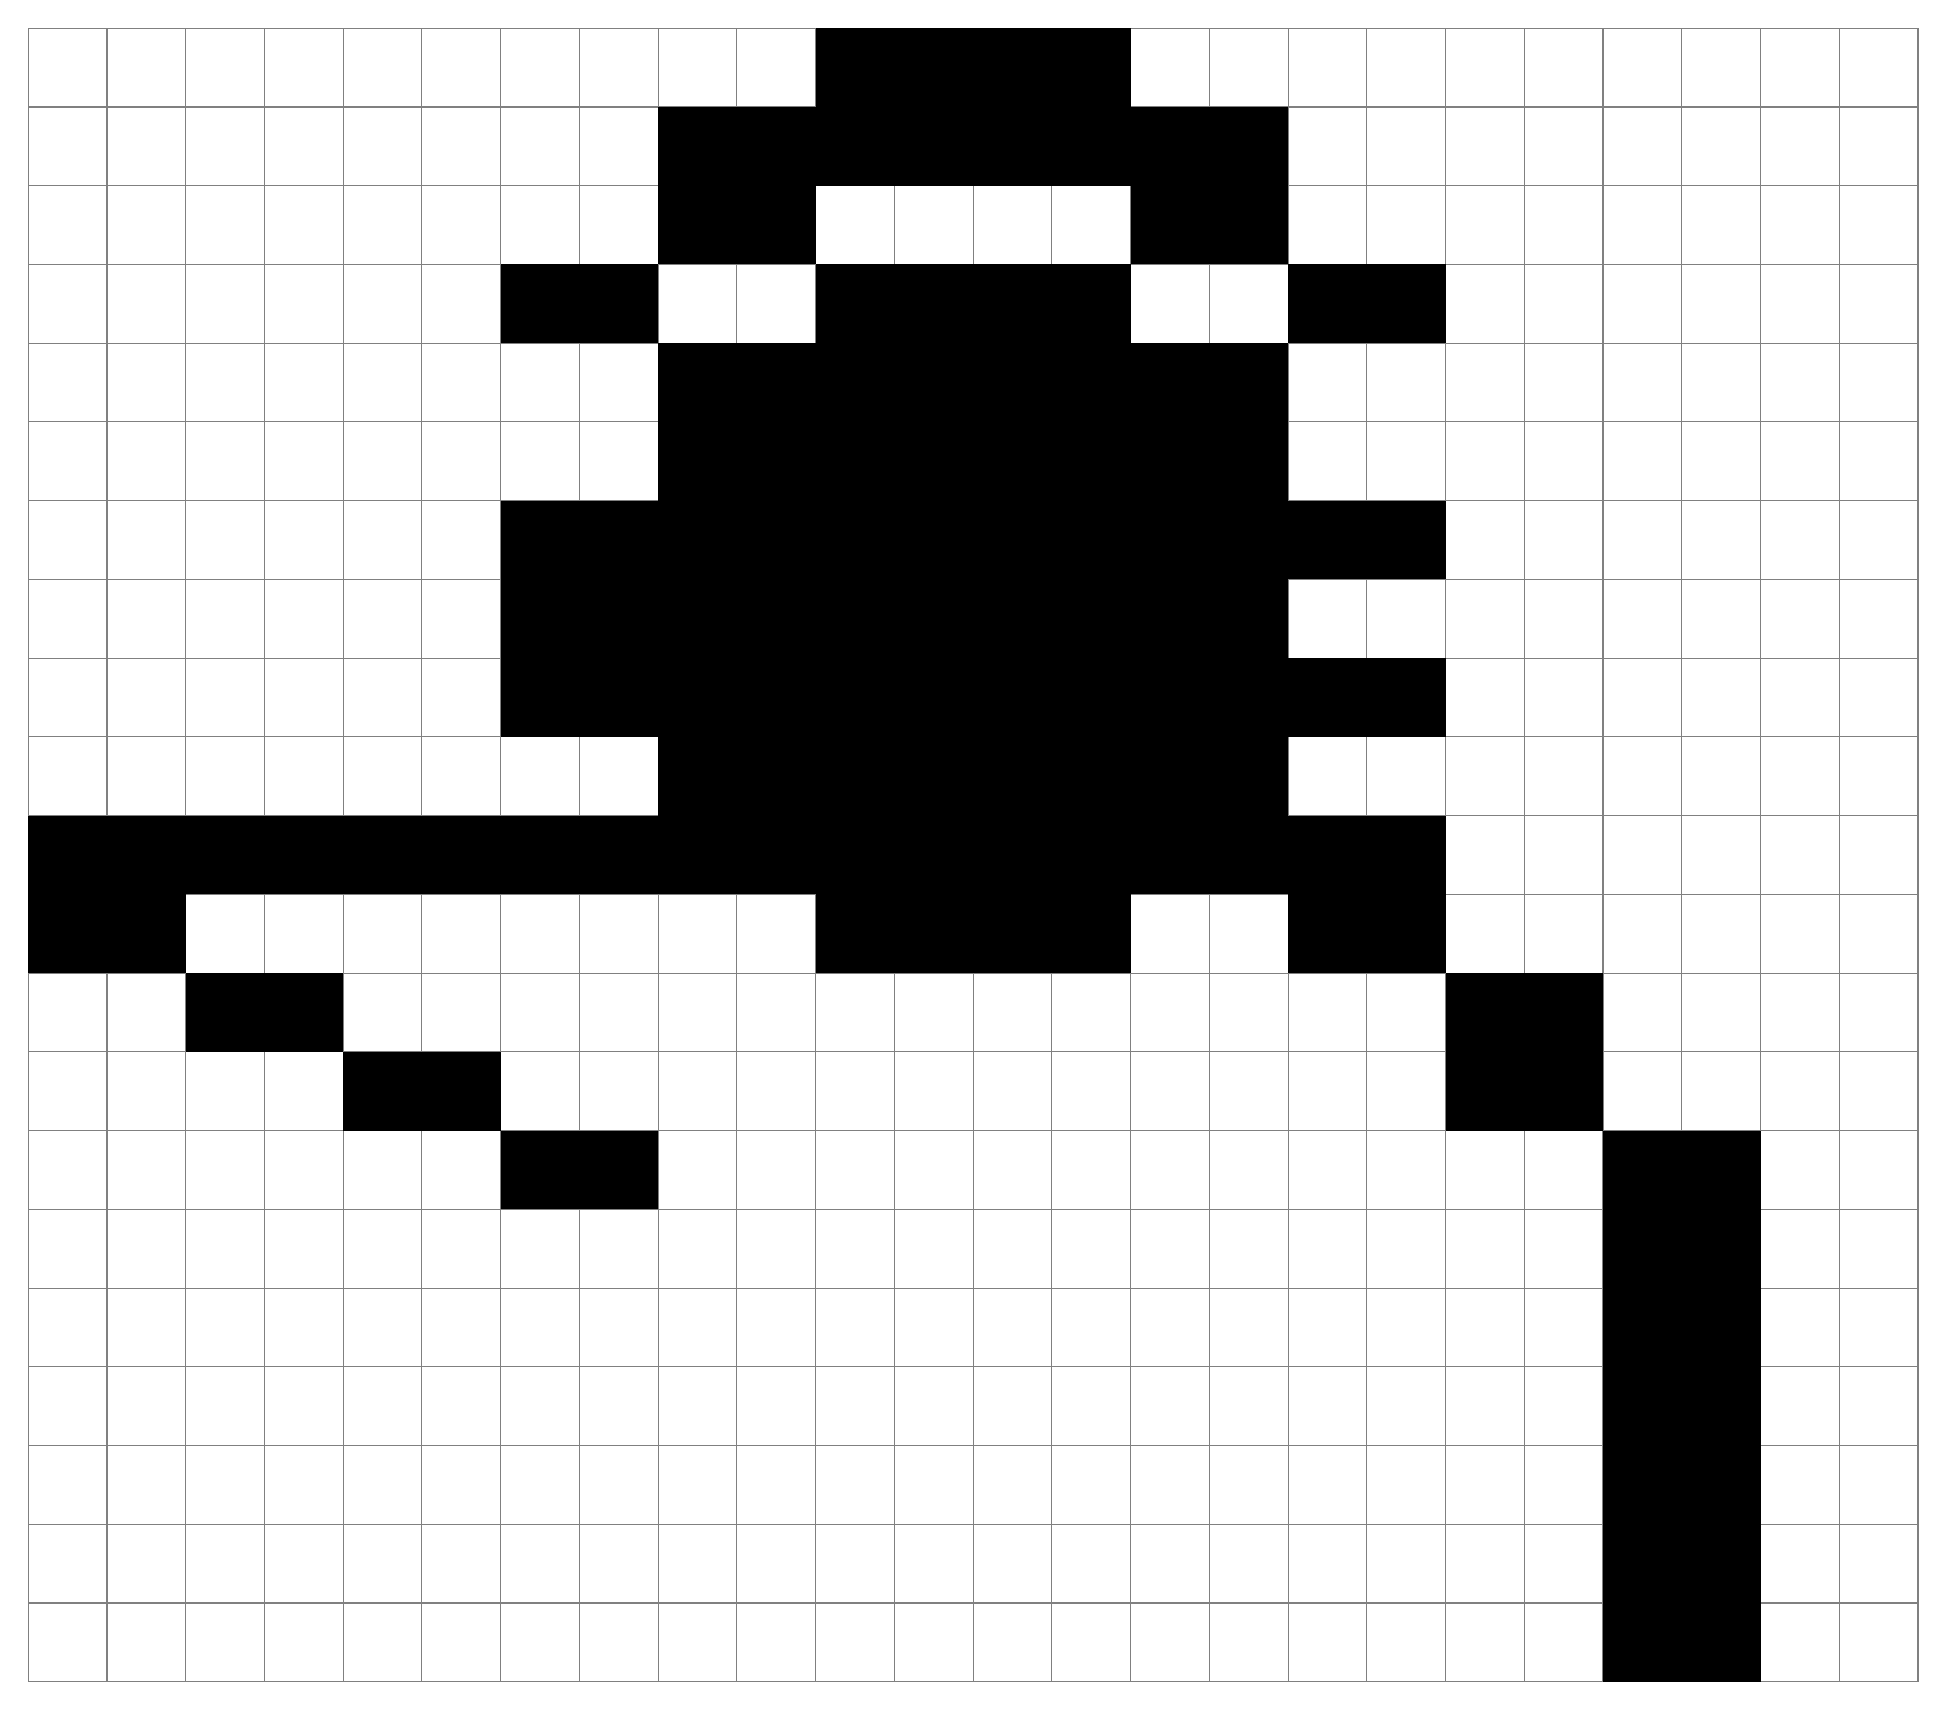
\begin{tikzpicture}

	\draw[step=1.0,gray,thin] (0,0) grid (24,21);
	\fill[\SPRITECOLOR] (10,20) rectangle ++ (1,1);
	\fill[\SPRITECOLOR] (11,20) rectangle ++ (1,1);
	\fill[\SPRITECOLOR] (12,20) rectangle ++ (1,1);
	\fill[\SPRITECOLOR] (13,20) rectangle ++ (1,1);
	\fill[\SPRITECOLOR] (8,19) rectangle ++ (1,1);
	\fill[\SPRITECOLOR] (9,19) rectangle ++ (1,1);
	\fill[\SPRITECOLOR] (10,19) rectangle ++ (1,1);
	\fill[\SPRITECOLOR] (11,19) rectangle ++ (1,1);
	\fill[\SPRITECOLOR] (12,19) rectangle ++ (1,1);
	\fill[\SPRITECOLOR] (13,19) rectangle ++ (1,1);
	\fill[\SPRITECOLOR] (14,19) rectangle ++ (1,1);
	\fill[\SPRITECOLOR] (15,19) rectangle ++ (1,1);
	\fill[\SPRITECOLOR] (8,18) rectangle ++ (1,1);
	\fill[\SPRITECOLOR] (9,18) rectangle ++ (1,1);
	\fill[\SPRITECOLOR] (14,18) rectangle ++ (1,1);
	\fill[\SPRITECOLOR] (15,18) rectangle ++ (1,1);
	\fill[\SPRITECOLOR] (6,17) rectangle ++ (1,1);
	\fill[\SPRITECOLOR] (7,17) rectangle ++ (1,1);
	\fill[\SPRITECOLOR] (10,17) rectangle ++ (1,1);
	\fill[\SPRITECOLOR] (11,17) rectangle ++ (1,1);
	\fill[\SPRITECOLOR] (12,17) rectangle ++ (1,1);
	\fill[\SPRITECOLOR] (13,17) rectangle ++ (1,1);
	\fill[\SPRITECOLOR] (16,17) rectangle ++ (1,1);
	\fill[\SPRITECOLOR] (17,17) rectangle ++ (1,1);
	\fill[\SPRITECOLOR] (8,16) rectangle ++ (1,1);
	\fill[\SPRITECOLOR] (9,16) rectangle ++ (1,1);
	\fill[\MULTICOLORTWO] (10,16) rectangle ++ (1,1);
	\fill[\MULTICOLORTWO] (11,16) rectangle ++ (1,1);
	\fill[\SPRITECOLOR] (12,16) rectangle ++ (1,1);
	\fill[\SPRITECOLOR] (13,16) rectangle ++ (1,1);
	\fill[\SPRITECOLOR] (14,16) rectangle ++ (1,1);
	\fill[\SPRITECOLOR] (15,16) rectangle ++ (1,1);
	\fill[\MULTICOLORTWO] (8,15) rectangle ++ (1,1);
	\fill[\MULTICOLORTWO] (9,15) rectangle ++ (1,1);
	\fill[\SPRITECOLOR] (10,15) rectangle ++ (1,1);
	\fill[\SPRITECOLOR] (11,15) rectangle ++ (1,1);
	\fill[\SPRITECOLOR] (12,15) rectangle ++ (1,1);
	\fill[\SPRITECOLOR] (13,15) rectangle ++ (1,1);
	\fill[\SPRITECOLOR] (14,15) rectangle ++ (1,1);
	\fill[\SPRITECOLOR] (15,15) rectangle ++ (1,1);
	\fill[\SPRITECOLOR] (6,14) rectangle ++ (1,1);
	\fill[\SPRITECOLOR] (7,14) rectangle ++ (1,1);
	\fill[\SPRITECOLOR] (8,14) rectangle ++ (1,1);
	\fill[\SPRITECOLOR] (9,14) rectangle ++ (1,1);
	\fill[\SPRITECOLOR] (10,14) rectangle ++ (1,1);
	\fill[\SPRITECOLOR] (11,14) rectangle ++ (1,1);
	\fill[\SPRITECOLOR] (12,14) rectangle ++ (1,1);
	\fill[\SPRITECOLOR] (13,14) rectangle ++ (1,1);
	\fill[\MULTICOLORTWO] (14,14) rectangle ++ (1,1);
	\fill[\MULTICOLORTWO] (15,14) rectangle ++ (1,1);
	\fill[\MULTICOLORTWO] (16,14) rectangle ++ (1,1);
	\fill[\MULTICOLORTWO] (17,14) rectangle ++ (1,1);
	\fill[\SPRITECOLOR] (6,13) rectangle ++ (1,1);
	\fill[\SPRITECOLOR] (7,13) rectangle ++ (1,1);
	\fill[\SPRITECOLOR] (8,13) rectangle ++ (1,1);
	\fill[\SPRITECOLOR] (9,13) rectangle ++ (1,1);
	\fill[\SPRITECOLOR] (10,13) rectangle ++ (1,1);
	\fill[\SPRITECOLOR] (11,13) rectangle ++ (1,1);
	\fill[\SPRITECOLOR] (12,13) rectangle ++ (1,1);
	\fill[\SPRITECOLOR] (13,13) rectangle ++ (1,1);
	\fill[\MULTICOLORTWO] (14,13) rectangle ++ (1,1);
	\fill[\MULTICOLORTWO] (15,13) rectangle ++ (1,1);
	\fill[\SPRITECOLOR] (6,12) rectangle ++ (1,1);
	\fill[\SPRITECOLOR] (7,12) rectangle ++ (1,1);
	\fill[\SPRITECOLOR] (8,12) rectangle ++ (1,1);
	\fill[\SPRITECOLOR] (9,12) rectangle ++ (1,1);
	\fill[\SPRITECOLOR] (10,12) rectangle ++ (1,1);
	\fill[\SPRITECOLOR] (11,12) rectangle ++ (1,1);
	\fill[\SPRITECOLOR] (12,12) rectangle ++ (1,1);
	\fill[\SPRITECOLOR] (13,12) rectangle ++ (1,1);
	\fill[\MULTICOLORTWO] (14,12) rectangle ++ (1,1);
	\fill[\MULTICOLORTWO] (15,12) rectangle ++ (1,1);
	\fill[\MULTICOLORTWO] (16,12) rectangle ++ (1,1);
	\fill[\MULTICOLORTWO] (17,12) rectangle ++ (1,1);
	\fill[\SPRITECOLOR] (8,11) rectangle ++ (1,1);
	\fill[\SPRITECOLOR] (9,11) rectangle ++ (1,1);
	\fill[\SPRITECOLOR] (10,11) rectangle ++ (1,1);
	\fill[\SPRITECOLOR] (11,11) rectangle ++ (1,1);
	\fill[\SPRITECOLOR] (12,11) rectangle ++ (1,1);
	\fill[\SPRITECOLOR] (13,11) rectangle ++ (1,1);
	\fill[\SPRITECOLOR] (14,11) rectangle ++ (1,1);
	\fill[\SPRITECOLOR] (15,11) rectangle ++ (1,1);
	\fill[\MULTICOLORTWO] (0,10) rectangle ++ (1,1);
	\fill[\MULTICOLORTWO] (1,10) rectangle ++ (1,1);
	\fill[\MULTICOLORONE] (2,10) rectangle ++ (1,1);
	\fill[\MULTICOLORONE] (3,10) rectangle ++ (1,1);
	\fill[\MULTICOLORONE] (4,10) rectangle ++ (1,1);
	\fill[\MULTICOLORONE] (5,10) rectangle ++ (1,1);
	\fill[\MULTICOLORONE] (6,10) rectangle ++ (1,1);
	\fill[\MULTICOLORONE] (7,10) rectangle ++ (1,1);
	\fill[\SPRITECOLOR] (8,10) rectangle ++ (1,1);
	\fill[\SPRITECOLOR] (9,10) rectangle ++ (1,1);
	\fill[\SPRITECOLOR] (10,10) rectangle ++ (1,1);
	\fill[\SPRITECOLOR] (11,10) rectangle ++ (1,1);
	\fill[\SPRITECOLOR] (12,10) rectangle ++ (1,1);
	\fill[\SPRITECOLOR] (13,10) rectangle ++ (1,1);
	\fill[\SPRITECOLOR] (14,10) rectangle ++ (1,1);
	\fill[\SPRITECOLOR] (15,10) rectangle ++ (1,1);
	\fill[\MULTICOLORONE] (16,10) rectangle ++ (1,1);
	\fill[\MULTICOLORONE] (17,10) rectangle ++ (1,1);
	\fill[\MULTICOLORONE] (0,9) rectangle ++ (1,1);
	\fill[\MULTICOLORONE] (1,9) rectangle ++ (1,1);
	\fill[\SPRITECOLOR] (10,9) rectangle ++ (1,1);
	\fill[\SPRITECOLOR] (11,9) rectangle ++ (1,1);
	\fill[\SPRITECOLOR] (12,9) rectangle ++ (1,1);
	\fill[\SPRITECOLOR] (13,9) rectangle ++ (1,1);
	\fill[\MULTICOLORONE] (16,9) rectangle ++ (1,1);
	\fill[\MULTICOLORONE] (17,9) rectangle ++ (1,1);
	\fill[\MULTICOLORONE] (2,8) rectangle ++ (1,1);
	\fill[\MULTICOLORONE] (3,8) rectangle ++ (1,1);
	\fill[\MULTICOLORONE] (18,8) rectangle ++ (1,1);
	\fill[\MULTICOLORONE] (19,8) rectangle ++ (1,1);
	\fill[\MULTICOLORONE] (4,7) rectangle ++ (1,1);
	\fill[\MULTICOLORONE] (5,7) rectangle ++ (1,1);
	\fill[\MULTICOLORONE] (18,7) rectangle ++ (1,1);
	\fill[\MULTICOLORONE] (19,7) rectangle ++ (1,1);
	\fill[\MULTICOLORONE] (6,6) rectangle ++ (1,1);
	\fill[\MULTICOLORONE] (7,6) rectangle ++ (1,1);
	\fill[\MULTICOLORTWO] (20,6) rectangle ++ (1,1);
	\fill[\MULTICOLORTWO] (21,6) rectangle ++ (1,1);
	\fill[\MULTICOLORONE] (20,5) rectangle ++ (1,1);
	\fill[\MULTICOLORONE] (21,5) rectangle ++ (1,1);
	\fill[\MULTICOLORONE] (20,4) rectangle ++ (1,1);
	\fill[\MULTICOLORONE] (21,4) rectangle ++ (1,1);
	\fill[\MULTICOLORONE] (20,3) rectangle ++ (1,1);
	\fill[\MULTICOLORONE] (21,3) rectangle ++ (1,1);
	\fill[\MULTICOLORONE] (20,2) rectangle ++ (1,1);
	\fill[\MULTICOLORONE] (21,2) rectangle ++ (1,1);
	\fill[\MULTICOLORONE] (20,1) rectangle ++ (1,1);
	\fill[\MULTICOLORONE] (21,1) rectangle ++ (1,1);
	\fill[\MULTICOLORONE] (20,0) rectangle ++ (1,1);
	\fill[\MULTICOLORONE] (21,0) rectangle ++ (1,1);

      \end{tikzpicture}
    \end{adjustbox}
  }\caption{LAND\_GILBY6}
\end{figure}

	\end{subfigure}
} & 
\makecell[l]{
	\begin{subfigure}{0.3\textwidth}
    \def\MULTICOLORONE{gray}
    \def\MULTICOLORTWO{white}
    \def\SPRITECOLOR{purple}
		
\begin{figure}[H]
  {
    \setlength{\tabcolsep}{3.0pt}
    \setlength\cmidrulewidth{\heavyrulewidth} % Make cmidrule = 
    \begin{adjustbox}{width=3cm,center}
      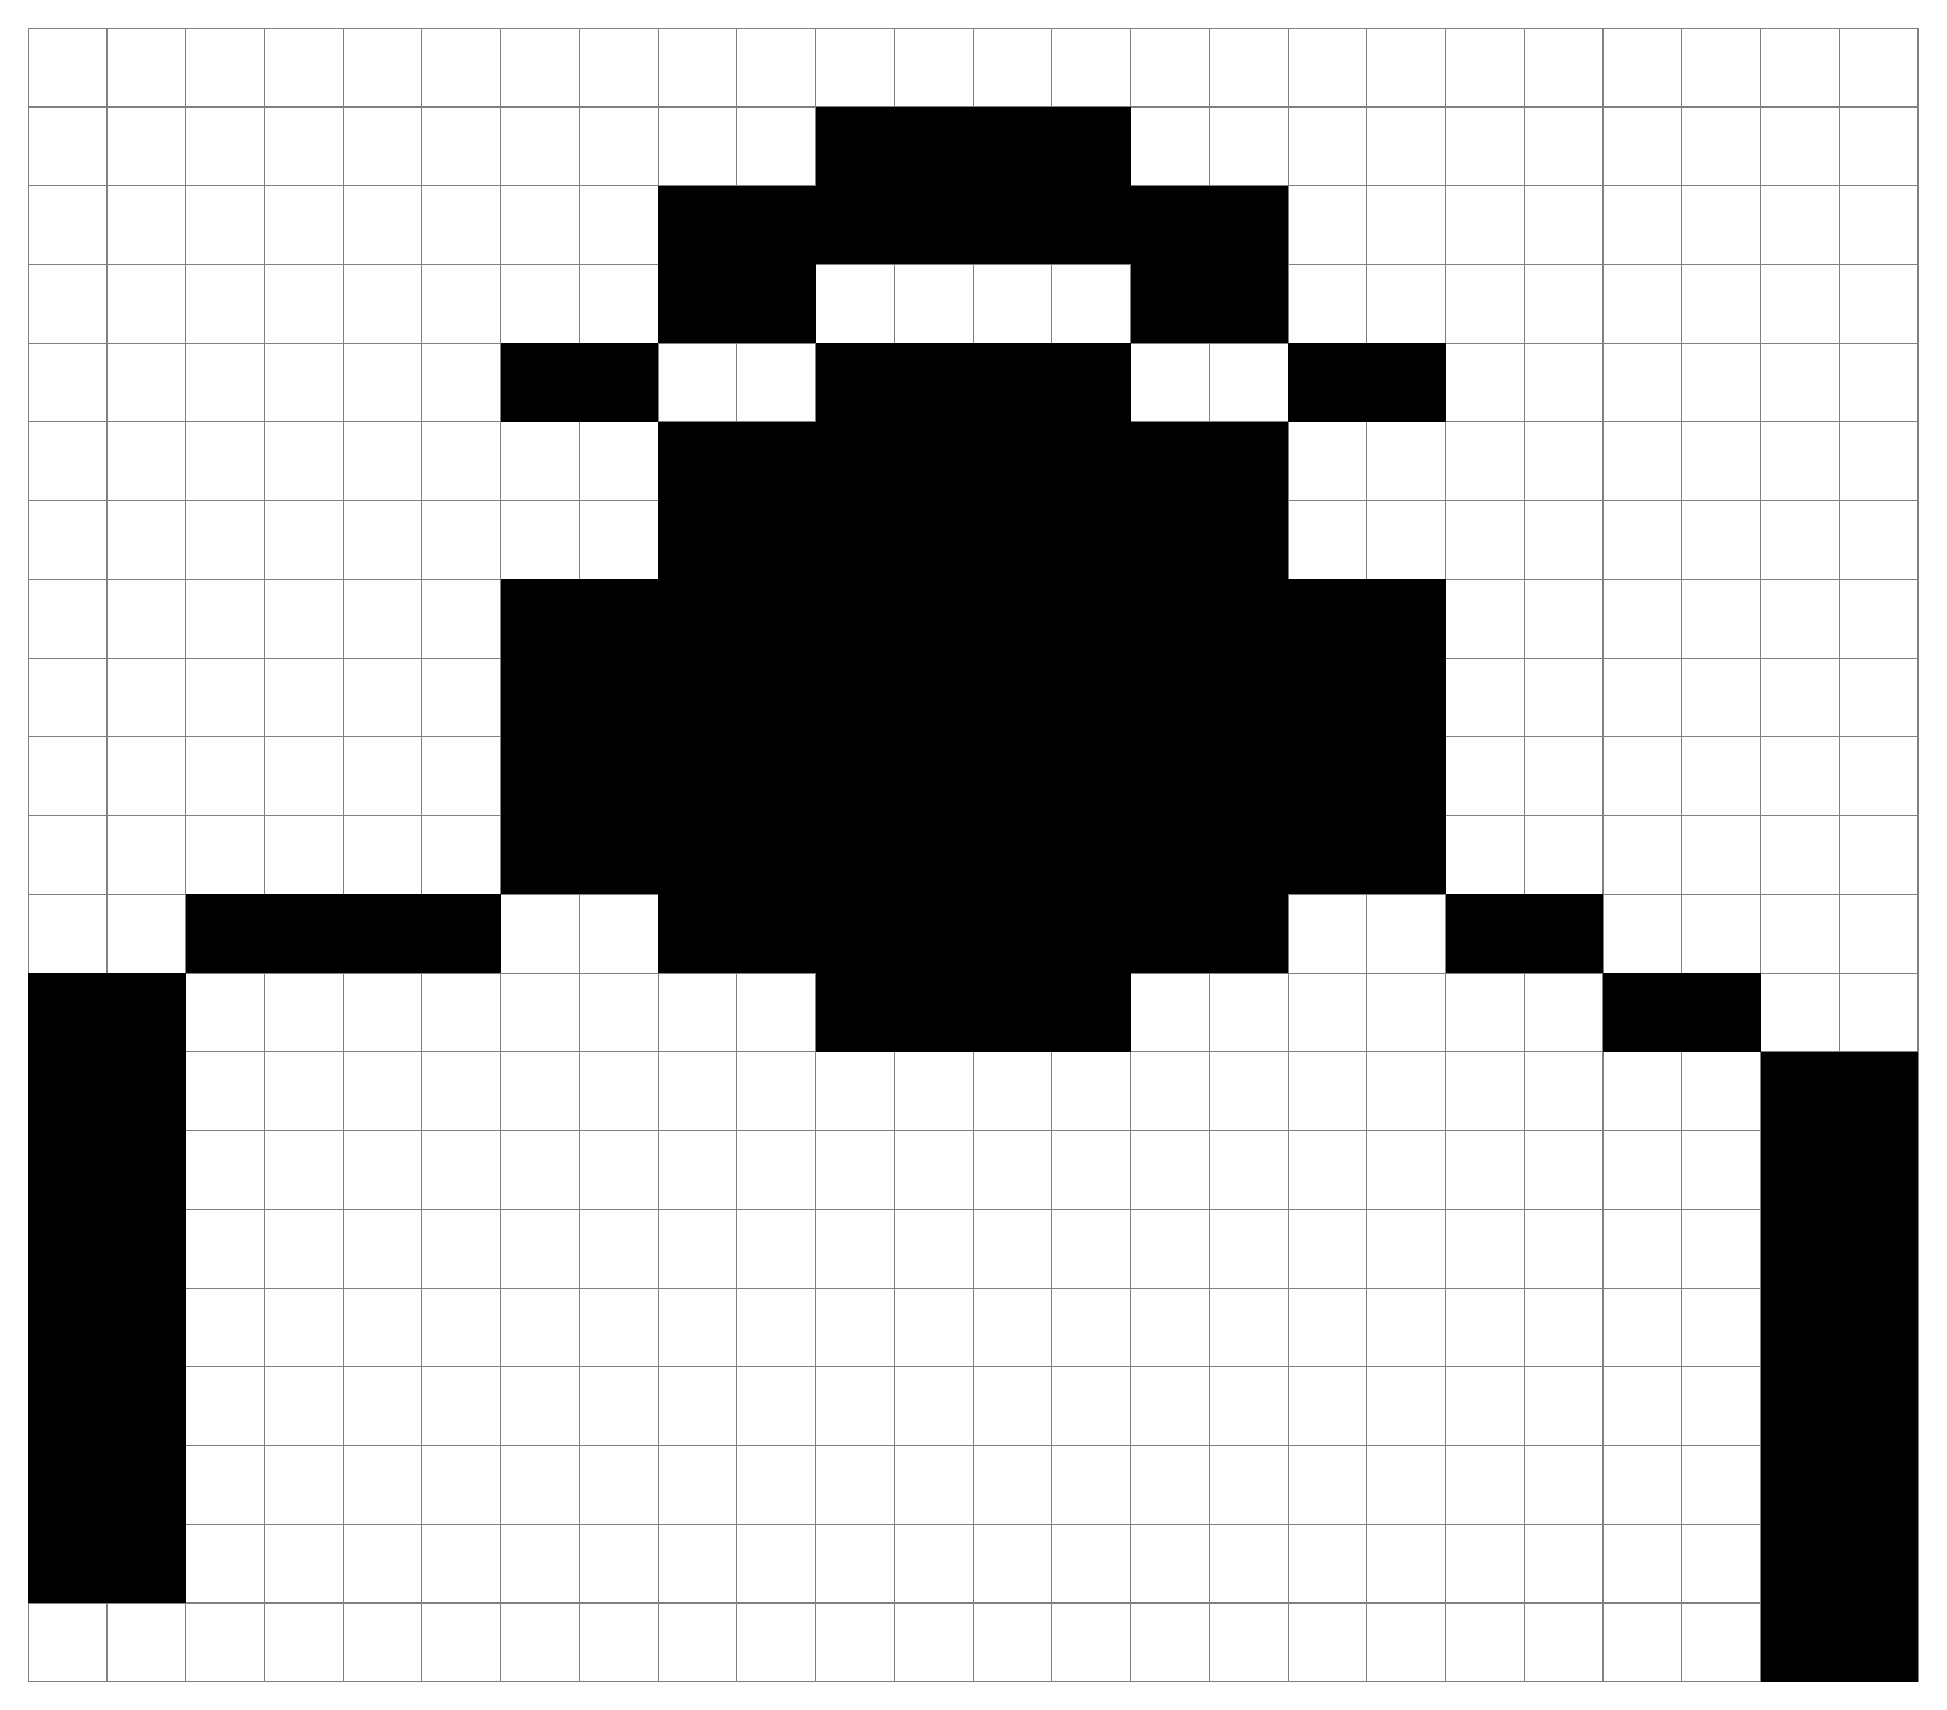
\begin{tikzpicture}

	\draw[step=1.0,gray,thin] (0,0) grid (24,21);
	\fill[\SPRITECOLOR] (10,19) rectangle ++ (1,1);
	\fill[\SPRITECOLOR] (11,19) rectangle ++ (1,1);
	\fill[\SPRITECOLOR] (12,19) rectangle ++ (1,1);
	\fill[\SPRITECOLOR] (13,19) rectangle ++ (1,1);
	\fill[\SPRITECOLOR] (8,18) rectangle ++ (1,1);
	\fill[\SPRITECOLOR] (9,18) rectangle ++ (1,1);
	\fill[\SPRITECOLOR] (10,18) rectangle ++ (1,1);
	\fill[\SPRITECOLOR] (11,18) rectangle ++ (1,1);
	\fill[\SPRITECOLOR] (12,18) rectangle ++ (1,1);
	\fill[\SPRITECOLOR] (13,18) rectangle ++ (1,1);
	\fill[\SPRITECOLOR] (14,18) rectangle ++ (1,1);
	\fill[\SPRITECOLOR] (15,18) rectangle ++ (1,1);
	\fill[\SPRITECOLOR] (8,17) rectangle ++ (1,1);
	\fill[\SPRITECOLOR] (9,17) rectangle ++ (1,1);
	\fill[\SPRITECOLOR] (14,17) rectangle ++ (1,1);
	\fill[\SPRITECOLOR] (15,17) rectangle ++ (1,1);
	\fill[\SPRITECOLOR] (6,16) rectangle ++ (1,1);
	\fill[\SPRITECOLOR] (7,16) rectangle ++ (1,1);
	\fill[\SPRITECOLOR] (10,16) rectangle ++ (1,1);
	\fill[\SPRITECOLOR] (11,16) rectangle ++ (1,1);
	\fill[\SPRITECOLOR] (12,16) rectangle ++ (1,1);
	\fill[\SPRITECOLOR] (13,16) rectangle ++ (1,1);
	\fill[\SPRITECOLOR] (16,16) rectangle ++ (1,1);
	\fill[\SPRITECOLOR] (17,16) rectangle ++ (1,1);
	\fill[\SPRITECOLOR] (8,15) rectangle ++ (1,1);
	\fill[\SPRITECOLOR] (9,15) rectangle ++ (1,1);
	\fill[\MULTICOLORTWO] (10,15) rectangle ++ (1,1);
	\fill[\MULTICOLORTWO] (11,15) rectangle ++ (1,1);
	\fill[\SPRITECOLOR] (12,15) rectangle ++ (1,1);
	\fill[\SPRITECOLOR] (13,15) rectangle ++ (1,1);
	\fill[\SPRITECOLOR] (14,15) rectangle ++ (1,1);
	\fill[\SPRITECOLOR] (15,15) rectangle ++ (1,1);
	\fill[\MULTICOLORTWO] (8,14) rectangle ++ (1,1);
	\fill[\MULTICOLORTWO] (9,14) rectangle ++ (1,1);
	\fill[\SPRITECOLOR] (10,14) rectangle ++ (1,1);
	\fill[\SPRITECOLOR] (11,14) rectangle ++ (1,1);
	\fill[\SPRITECOLOR] (12,14) rectangle ++ (1,1);
	\fill[\SPRITECOLOR] (13,14) rectangle ++ (1,1);
	\fill[\SPRITECOLOR] (14,14) rectangle ++ (1,1);
	\fill[\SPRITECOLOR] (15,14) rectangle ++ (1,1);
	\fill[\SPRITECOLOR] (6,13) rectangle ++ (1,1);
	\fill[\SPRITECOLOR] (7,13) rectangle ++ (1,1);
	\fill[\SPRITECOLOR] (8,13) rectangle ++ (1,1);
	\fill[\SPRITECOLOR] (9,13) rectangle ++ (1,1);
	\fill[\SPRITECOLOR] (10,13) rectangle ++ (1,1);
	\fill[\SPRITECOLOR] (11,13) rectangle ++ (1,1);
	\fill[\SPRITECOLOR] (12,13) rectangle ++ (1,1);
	\fill[\SPRITECOLOR] (13,13) rectangle ++ (1,1);
	\fill[\SPRITECOLOR] (14,13) rectangle ++ (1,1);
	\fill[\SPRITECOLOR] (15,13) rectangle ++ (1,1);
	\fill[\SPRITECOLOR] (16,13) rectangle ++ (1,1);
	\fill[\SPRITECOLOR] (17,13) rectangle ++ (1,1);
	\fill[\SPRITECOLOR] (6,12) rectangle ++ (1,1);
	\fill[\SPRITECOLOR] (7,12) rectangle ++ (1,1);
	\fill[\SPRITECOLOR] (8,12) rectangle ++ (1,1);
	\fill[\SPRITECOLOR] (9,12) rectangle ++ (1,1);
	\fill[\SPRITECOLOR] (10,12) rectangle ++ (1,1);
	\fill[\SPRITECOLOR] (11,12) rectangle ++ (1,1);
	\fill[\SPRITECOLOR] (12,12) rectangle ++ (1,1);
	\fill[\SPRITECOLOR] (13,12) rectangle ++ (1,1);
	\fill[\SPRITECOLOR] (14,12) rectangle ++ (1,1);
	\fill[\SPRITECOLOR] (15,12) rectangle ++ (1,1);
	\fill[\SPRITECOLOR] (16,12) rectangle ++ (1,1);
	\fill[\SPRITECOLOR] (17,12) rectangle ++ (1,1);
	\fill[\SPRITECOLOR] (6,11) rectangle ++ (1,1);
	\fill[\SPRITECOLOR] (7,11) rectangle ++ (1,1);
	\fill[\SPRITECOLOR] (8,11) rectangle ++ (1,1);
	\fill[\SPRITECOLOR] (9,11) rectangle ++ (1,1);
	\fill[\SPRITECOLOR] (10,11) rectangle ++ (1,1);
	\fill[\SPRITECOLOR] (11,11) rectangle ++ (1,1);
	\fill[\SPRITECOLOR] (12,11) rectangle ++ (1,1);
	\fill[\SPRITECOLOR] (13,11) rectangle ++ (1,1);
	\fill[\SPRITECOLOR] (14,11) rectangle ++ (1,1);
	\fill[\SPRITECOLOR] (15,11) rectangle ++ (1,1);
	\fill[\SPRITECOLOR] (16,11) rectangle ++ (1,1);
	\fill[\SPRITECOLOR] (17,11) rectangle ++ (1,1);
	\fill[\MULTICOLORONE] (6,10) rectangle ++ (1,1);
	\fill[\MULTICOLORONE] (7,10) rectangle ++ (1,1);
	\fill[\SPRITECOLOR] (8,10) rectangle ++ (1,1);
	\fill[\SPRITECOLOR] (9,10) rectangle ++ (1,1);
	\fill[\SPRITECOLOR] (10,10) rectangle ++ (1,1);
	\fill[\SPRITECOLOR] (11,10) rectangle ++ (1,1);
	\fill[\SPRITECOLOR] (12,10) rectangle ++ (1,1);
	\fill[\SPRITECOLOR] (13,10) rectangle ++ (1,1);
	\fill[\SPRITECOLOR] (14,10) rectangle ++ (1,1);
	\fill[\SPRITECOLOR] (15,10) rectangle ++ (1,1);
	\fill[\MULTICOLORONE] (16,10) rectangle ++ (1,1);
	\fill[\MULTICOLORONE] (17,10) rectangle ++ (1,1);
	\fill[\MULTICOLORONE] (2,9) rectangle ++ (1,1);
	\fill[\MULTICOLORONE] (3,9) rectangle ++ (1,1);
	\fill[\MULTICOLORONE] (4,9) rectangle ++ (1,1);
	\fill[\MULTICOLORONE] (5,9) rectangle ++ (1,1);
	\fill[\SPRITECOLOR] (8,9) rectangle ++ (1,1);
	\fill[\SPRITECOLOR] (9,9) rectangle ++ (1,1);
	\fill[\SPRITECOLOR] (10,9) rectangle ++ (1,1);
	\fill[\SPRITECOLOR] (11,9) rectangle ++ (1,1);
	\fill[\SPRITECOLOR] (12,9) rectangle ++ (1,1);
	\fill[\SPRITECOLOR] (13,9) rectangle ++ (1,1);
	\fill[\SPRITECOLOR] (14,9) rectangle ++ (1,1);
	\fill[\SPRITECOLOR] (15,9) rectangle ++ (1,1);
	\fill[\MULTICOLORONE] (18,9) rectangle ++ (1,1);
	\fill[\MULTICOLORONE] (19,9) rectangle ++ (1,1);
	\fill[\MULTICOLORTWO] (0,8) rectangle ++ (1,1);
	\fill[\MULTICOLORTWO] (1,8) rectangle ++ (1,1);
	\fill[\SPRITECOLOR] (10,8) rectangle ++ (1,1);
	\fill[\SPRITECOLOR] (11,8) rectangle ++ (1,1);
	\fill[\SPRITECOLOR] (12,8) rectangle ++ (1,1);
	\fill[\SPRITECOLOR] (13,8) rectangle ++ (1,1);
	\fill[\MULTICOLORONE] (20,8) rectangle ++ (1,1);
	\fill[\MULTICOLORONE] (21,8) rectangle ++ (1,1);
	\fill[\MULTICOLORONE] (0,7) rectangle ++ (1,1);
	\fill[\MULTICOLORONE] (1,7) rectangle ++ (1,1);
	\fill[\MULTICOLORTWO] (22,7) rectangle ++ (1,1);
	\fill[\MULTICOLORTWO] (23,7) rectangle ++ (1,1);
	\fill[\MULTICOLORONE] (0,6) rectangle ++ (1,1);
	\fill[\MULTICOLORONE] (1,6) rectangle ++ (1,1);
	\fill[\MULTICOLORONE] (22,6) rectangle ++ (1,1);
	\fill[\MULTICOLORONE] (23,6) rectangle ++ (1,1);
	\fill[\MULTICOLORONE] (0,5) rectangle ++ (1,1);
	\fill[\MULTICOLORONE] (1,5) rectangle ++ (1,1);
	\fill[\MULTICOLORONE] (22,5) rectangle ++ (1,1);
	\fill[\MULTICOLORONE] (23,5) rectangle ++ (1,1);
	\fill[\MULTICOLORONE] (0,4) rectangle ++ (1,1);
	\fill[\MULTICOLORONE] (1,4) rectangle ++ (1,1);
	\fill[\MULTICOLORONE] (22,4) rectangle ++ (1,1);
	\fill[\MULTICOLORONE] (23,4) rectangle ++ (1,1);
	\fill[\MULTICOLORONE] (0,3) rectangle ++ (1,1);
	\fill[\MULTICOLORONE] (1,3) rectangle ++ (1,1);
	\fill[\MULTICOLORONE] (22,3) rectangle ++ (1,1);
	\fill[\MULTICOLORONE] (23,3) rectangle ++ (1,1);
	\fill[\MULTICOLORONE] (0,2) rectangle ++ (1,1);
	\fill[\MULTICOLORONE] (1,2) rectangle ++ (1,1);
	\fill[\MULTICOLORONE] (22,2) rectangle ++ (1,1);
	\fill[\MULTICOLORONE] (23,2) rectangle ++ (1,1);
	\fill[\MULTICOLORONE] (0,1) rectangle ++ (1,1);
	\fill[\MULTICOLORONE] (1,1) rectangle ++ (1,1);
	\fill[\MULTICOLORONE] (22,1) rectangle ++ (1,1);
	\fill[\MULTICOLORONE] (23,1) rectangle ++ (1,1);
	\fill[\MULTICOLORONE] (22,0) rectangle ++ (1,1);
	\fill[\MULTICOLORONE] (23,0) rectangle ++ (1,1);

      \end{tikzpicture}
    \end{adjustbox}
  }\caption{LAND\_GILBY7}
\end{figure}

	\end{subfigure}
} \\ 
        \addlinespace
        \bottomrule
      \end{tabular}
    \end{adjustbox}
  }\caption{The sprites used by the top half of the screen and the bottom half of the screen.}
\end{figure}
